\documentclass[screen=true, 10pt, acmsmall]{acmart}
\usepackage[utf8]{inputenc}
\usepackage[T1]{fontenc}

\newcommand{\packageGraphicx}{\usepackage{graphicx}}
\newcommand{\packageHyperref}{\usepackage{hyperref}}
\newcommand{\renewrmdefault}{\renewcommand{\rmdefault}{ptm}}
\newcommand{\packageRelsize}{\usepackage{relsize}}
\newcommand{\packageMathabx}{\usepackage{mathabx}}
% Avoid conflicts between "mathabx" and "wasysym":
\newcommand{\packageWasysym}{
  \let\leftmoon\relax \let\rightmoon\relax \let\fullmoon\relax \let\newmoon\relax \let\diameter\relax
  \usepackage{wasysym}}
\newcommand{\packageTextcomp}{\usepackage{textcomp}}
\newcommand{\packageFramed}{\usepackage{framed}}
\newcommand{\packageHyphenat}{\usepackage[htt]{hyphenat}}
\newcommand{\packageColor}{\usepackage[usenames,dvipsnames]{color}}
\newcommand{\doHypersetup}{\hypersetup{bookmarks=true,bookmarksopen=true,bookmarksnumbered=true}}
\newcommand{\packageTocstyle}{\IfFileExists{tocstyle.sty}{\usepackage{tocstyle}\usetocstyle{standard}}{}}
\newcommand{\packageCJK}{\IfFileExists{CJK.sty}{\usepackage{CJK}}{}}
%%%%%%%%%%%%%%%%%%%%%%%%%%%%%%%%%%%%%%%%%%%%%%%%%%%%%%%%%%%%%%%%%%%%%%%%%%%%%%%%
% BEGIN acmart-load.tex
% Avoid package option conflict
\renewcommand\packageColor\relax
\renewcommand\packageTocstyle\relax
\renewcommand\packageMathabx{\ifx\bigtimes\undefined \usepackage{mathabx} \else \relax \fi}
% Both 'mathabx' and 'newtxmath' (required by the 'acmart' class) define a '\bigtimes' command. 
\let\Footnote\undefined
\let\captionwidth\undefined
\renewcommand{\renewrmdefault}{}
% END acmart-load.tex
%%%%%%%%%%%%%%%%%%%%%%%%%%%%%%%%%%%%%%%%%%%%%%%%%%%%%%%%%%%%%%%%%%%%%%%%%%%%%%%%
% This is the default style configuration for Scribble-generated Latex

\packageGraphicx
\packageHyperref
\renewrmdefault
\packageRelsize
\packageMathabx
\packageWasysym
\packageTextcomp
\packageFramed
\packageHyphenat
\packageColor
\doHypersetup
\packageTocstyle
\packageCJK


%%%%%%%%%%%%%%%%%%%%%%%%%%%%%%%%%%%%%%%%%%%%%%%%%%%%%%%%%%%%%%%%%%%%%%%%%%%%%%%%
% Configuration that is especially meant to be overridden:

% Inserted before every ``chapter'', useful for starting each one on a new page:
\newcommand{\sectionNewpage}{}
% Inserted before every book ``part''
\newcommand{\partNewpage}{\sectionNewpage}

% Hooks for actions within the `document' environment:
\newcommand{\preDoc}{}
\newcommand{\postDoc}{}

% Generated by `secref'; first arg is section number, second is section title:
\newcommand{\BookRef}[2]{\emph{#2}}
\newcommand{\ChapRef}[2]{\SecRef{#1}{#2}}
\newcommand{\SecRef}[2]{section~#1}
\newcommand{\PartRef}[2]{part~#1}
% Generated by `Secref':
\newcommand{\BookRefUC}[2]{\BookRef{#1}{#2}}
\newcommand{\ChapRefUC}[2]{\SecRefUC{#1}{#2}}
\newcommand{\SecRefUC}[2]{Section~#1}
\newcommand{\PartRefUC}[2]{Part~#1}

% Variants of the above with a label for an internal reference:
\newcommand{\BookRefLocal}[3]{\hyperref[#1]{\BookRef{#2}{#3}}}
\newcommand{\ChapRefLocal}[3]{\hyperref[#1]{\ChapRef{#2}{#3}}}
\newcommand{\SecRefLocal}[3]{\hyperref[#1]{\SecRef{#2}{#3}}}
\newcommand{\PartRefLocal}[3]{\hyperref[#1]{\PartRef{#2}{#3}}}
\newcommand{\BookRefLocalUC}[3]{\hyperref[#1]{\BookRefUC{#2}{#3}}}
\newcommand{\ChapRefLocalUC}[3]{\hyperref[#1]{\ChapRefUC{#2}{#3}}}
\newcommand{\SecRefLocalUC}[3]{\hyperref[#1]{\SecRefUC{#2}{#3}}}
\newcommand{\PartRefLocalUC}[3]{\hyperref[#1]{\PartRefUC{#2}{#3}}}

% Variants of the above with a section number is empty (i.e., UnNumbered):
\newcommand{\BookRefUN}[1]{\BookRef{}{#1}}
\newcommand{\ChapRefUN}[1]{\SecRefUN{#1}}
\newcommand{\SecRefUN}[1]{``#1''}
\newcommand{\PartRefUN}[1]{\SecRefUN{#1}}
\newcommand{\BookRefUCUN}[1]{\BookRefUN{#1}}
\newcommand{\ChapRefUCUN}[1]{\ChapRefUN{#1}}
\newcommand{\SecRefUCUN}[1]{\SecRefUN{#1}}
\newcommand{\PartRefUCUN}[1]{\PartRefUN{#1}}

\newcommand{\BookRefLocalUN}[2]{\hyperref[#1]{\BookRefUN{#2}}}
\newcommand{\ChapRefLocalUN}[2]{\SecRefLocalUN{#1}{#2}}
\newcommand{\SecRefLocalUN}[2]{\hyperref[#1]{\SecRefUN{#2}}}
\newcommand{\PartRefLocalUN}[2]{\SecRefLocalUN{#1}{#2}}
\newcommand{\BookRefLocalUCUN}[2]{\BookRefLocalUN{#1}{#2}}
\newcommand{\ChapRefLocalUCUN}[2]{\ChapRefLocalUN{#1}{#2}}
\newcommand{\SecRefLocalUCUN}[2]{\SecRefLocalUN{#1}{#2}}
\newcommand{\PartRefLocalUCUN}[2]{\PartRefLocalUN{#1}{#2}}

\newcommand{\SectionNumberLink}[2]{\hyperref[#1]{#2}}

% Enabled with a 'enable-index-merge part style property. This default
% implementation isn't good enough, because the argument is a
% comma-separated sequence of labels:
\newcommand{\Smanypageref}[1]{\pageref{#1}}

%%%%%%%%%%%%%%%%%%%%%%%%%%%%%%%%%%%%%%%%%%%%%%%%%%%%%%%%%%%%%%%%%%%%%%%%%%%%%%%%
% Fonts

% Font commands used by generated text:
\newcommand{\Scribtexttt}[1]{{\texttt{#1}}}
\newcommand{\textsub}[1]{$_{\hbox{\textsmaller{#1}}}$}
\newcommand{\textsuper}[1]{$^{\hbox{\textsmaller{#1}}}$}
\newcommand{\intextcolor}[2]{\textcolor{#1}{#2}}
\newcommand{\intextrgbcolor}[2]{\textcolor[rgb]{#1}{#2}}
\newcommand{\incolorbox}[2]{{\fboxrule=0pt\fboxsep=0pt\colorbox{#1}{#2}}}
\newcommand{\inrgbcolorbox}[2]{{\fboxrule=0pt\fboxsep=0pt\colorbox[rgb]{#1}{#2}}}
\newcommand{\plainlink}[1]{#1}
\newcommand{\techoutside}[1]{#1}
\newcommand{\techinside}[1]{#1}
\newcommand{\badlink}[1]{#1}
\newcommand{\indexlink}[1]{#1}
\newcommand{\noborder}[1]{#1}
\newcommand{\Smaller}[1]{\textsmaller{#1}}
\newcommand{\Larger}[1]{\textlarger{#1}}
\newcommand{\planetName}[1]{PLane\hspace{-0.1ex}T}
\newcommand{\slant}[1]{{\textsl{#1}}}

% Used for <, >, and | in tt mode. For some fonts and installations,
% there seems to be an encoding issue, so pick T1 explicitly:
\newcommand{\Stttextmore}{{\fontencoding{T1}\selectfont>}}
\newcommand{\Stttextless}{{\fontencoding{T1}\selectfont<}}
\newcommand{\Stttextbar}{{\fontencoding{T1}\selectfont|}}

%%%%%%%%%%%%%%%%%%%%%%%%%%%%%%%%%%%%%%%%%%%%%%%%%%%%%%%%%%%%%%%%%%%%%%%%%%%%%%%%
% Tables

% The `stabular' environment seems to be the lesser of evils among 
%  page-breaking table environments (and we've made a copy as ``pltstabular'
%  to make sure that it doesn't change).

\makeatletter
%%%%%%%%%%%%%%%%%%%%%%%%%%%%%%%%%%%%%%%%%%%%%%%%%%%%%%%%%%%%%%%%%%%%%%
\message{pltstabular is a modification of stabular}
%% A renamed vsetion of:
%% stabular.sty
%% Copyright 1998 Sigitas Tolu\v sis
%% VTeX Ltd., Akademijos 4, Vilnius, Lithuania
%% e-mail sigitas@vtex.lt
%% http://www.vtex.lt/tex/download/macros/
%%
% This program can redistributed and/or modified under the terms
% of the LaTeX Project Public License Distributed from CTAN
% archives in directory macros/latex/base/lppl.txt; either
% version 1 of the License, or (at your option) any later version.
%
% PURPOSE:   Improve tabular environment.
%
% SHORT DESCRIPTION:
%
% Changed internal commands: \@mkpream, \@addamp, \@xhline
%
% Provides new commands in tabular (used after command \\):
% \emptyrow[#1] 
% -------------
%    Adds empty row, #1 - height of the row 
%
% \tabrow{#1}[#2] 
% ---------------
%    Adds row of natural height: #1\\[#2]
%
% Provides new environments: pltstabular and pltstabular* 
%                            --------     ---------
%            One more multi-page version of tabular
%
%
\def\empty@finalstrut#1{%
  \unskip\ifhmode\nobreak\fi\vrule\@width\z@\@height\z@\@depth\z@}
\def\no@strut{\global\setbox\@arstrutbox\hbox{%
    \vrule \@height\z@
           \@depth\z@
           \@width\z@}%
    \gdef\@endpbox{\empty@finalstrut\@arstrutbox\par\egroup\hfil}%
}%
\def\yes@strut{\global\setbox\@arstrutbox\hbox{%
    \vrule \@height\arraystretch \ht\strutbox
           \@depth\arraystretch \dp\strutbox
           \@width\z@}%
    \gdef\@endpbox{\@finalstrut\@arstrutbox\par\egroup\hfil}%
}%
\def\@mkpream#1{\@firstamptrue\@lastchclass6
  \let\@preamble\@empty\def\empty@preamble{\add@ins}%
  \let\protect\@unexpandable@protect
  \let\@sharp\relax\let\add@ins\relax
  \let\@startpbox\relax\let\@endpbox\relax
  \@expast{#1}%
  \expandafter\@tfor \expandafter
    \@nextchar \expandafter:\expandafter=\reserved@a\do
       {\@testpach\@nextchar
    \ifcase \@chclass \@classz \or \@classi \or \@classii \or \@classiii
      \or \@classiv \or\@classv \fi\@lastchclass\@chclass}%
  \ifcase \@lastchclass \@acol
      \or \or \@preamerr \@ne\or \@preamerr \tw@\or \or \@acol \fi}
\def\@addamp{%
  \if@firstamp
    \@firstampfalse
    \edef\empty@preamble{\add@ins}%
  \else
    \edef\@preamble{\@preamble &}%
    \edef\empty@preamble{\expandafter\noexpand\empty@preamble &\add@ins}%
  \fi}
\newif\iftw@hlines \tw@hlinesfalse
\def\@xhline{\ifx\reserved@a\hline
               \tw@hlinestrue
             \else\ifx\reserved@a\Hline
               \tw@hlinestrue
             \else
               \tw@hlinesfalse
             \fi\fi
      \iftw@hlines
        \aftergroup\do@after
      \fi
      \ifnum0=`{\fi}%
}
\def\do@after{\emptyrow[\the\doublerulesep]}
\def\emptyrow{\noalign\bgroup\@ifnextchar[\@emptyrow{\@emptyrow[\z@]}}
\def\@emptyrow[#1]{\no@strut\gdef\add@ins{\vrule \@height\z@ \@depth#1 \@width\z@}\egroup%
\empty@preamble\\
\noalign{\yes@strut\gdef\add@ins{\vrule \@height\z@ \@depth\z@ \@width\z@}}%
}
\def\tabrow#1{\noalign\bgroup\@ifnextchar[{\@tabrow{#1}}{\@tabrow{#1}[]}}
\def\@tabrow#1[#2]{\no@strut\egroup#1\ifx.#2.\\\else\\[#2]\fi\noalign{\yes@strut}}
%
\def\endpltstabular{\crcr\egroup\egroup \egroup}
\expandafter \let \csname endpltstabular*\endcsname = \endpltstabular
\def\pltstabular{\let\@halignto\@empty\@pltstabular}
\@namedef{pltstabular*}#1{\def\@halignto{to#1}\@pltstabular}
\def\@pltstabular{\leavevmode \bgroup \let\@acol\@tabacol
   \let\@classz\@tabclassz
   \let\@classiv\@tabclassiv \let\\\@tabularcr\@stabarray}
\def\@stabarray{\m@th\@ifnextchar[\@sarray{\@sarray[c]}}
\def\@sarray[#1]#2{%
  \bgroup
  \setbox\@arstrutbox\hbox{%
    \vrule \@height\arraystretch\ht\strutbox
           \@depth\arraystretch \dp\strutbox
           \@width\z@}%
  \@mkpream{#2}%
  \edef\@preamble{%
    \ialign \noexpand\@halignto
      \bgroup \@arstrut \@preamble \tabskip\z@skip \cr}%
  \let\@startpbox\@@startpbox \let\@endpbox\@@endpbox
  \let\tabularnewline\\%
%    \let\par\@empty
    \let\@sharp##%
    \set@typeset@protect
    \lineskip\z@skip\baselineskip\z@skip
    \@preamble}

%%%%%%%%%%%%%%%%%%%%%%%%%%%%%%%%%%%%%%%%%%%%%%%%%%%%%%%%%%%%%%%%%%%%%%
\makeatother

\newenvironment{bigtabular}{\begin{pltstabular}}{\end{pltstabular}}
% For the 'boxed table style:
\newcommand{\SBoxedLeft}{\textcolor[rgb]{0.6,0.6,1.0}{\vrule width 3pt\hspace{3pt}}}
% Formerly used to keep the horizontal line for a definition on the same page:
\newcommand{\SEndFirstHead}[0]{ \nopagebreak \\ }
% Corrects weirdness when a table is the first thing in
%  an itemization:
\newcommand{\bigtableinlinecorrect}[0]{~

\vspace{-\baselineskip}\vspace{\parskip}}
% Used to indent the table correctly in an itemization, since that's
%  one of the things stabular gets wrong:
\newlength{\stabLeft}
\newcommand{\bigtableleftpad}{\hspace{\stabLeft}}
\newcommand{\atItemizeStart}[0]{\addtolength{\stabLeft}{\labelsep}
                                \addtolength{\stabLeft}{\labelwidth}}


% For a single-column table in simple environments, it's better to
%  use the `list' environment instead of `stabular'.
\newenvironment{SingleColumn}{\begin{list}{}{\topsep=0pt\partopsep=0pt%
\listparindent=0pt\itemindent=0pt\labelwidth=0pt\leftmargin=0pt\rightmargin=0pt%
\itemsep=0pt\parsep=0pt}\item}{\end{list}}

%%%%%%%%%%%%%%%%%%%%%%%%%%%%%%%%%%%%%%%%%%%%%%%%%%%%%%%%%%%%%%%%%%%%%%%%%%%%%%%%
% Etc.

% ._ and .__
\newcommand{\Sendabbrev}[1]{#1\@}
\newcommand{\Sendsentence}[1]{\@#1}

% Default style for a nested flow:
\newenvironment{Subflow}{\begin{list}{}{\topsep=0pt\partopsep=0pt%
\listparindent=0pt\itemindent=0pt\labelwidth=0pt\leftmargin=0pt\rightmargin=0pt%
\itemsep=0pt}\item}{\end{list}}

% For the 'inset nested-flow style:
\newenvironment{SInsetFlow}{\begin{quote}}{\end{quote}}

% Indent a 'code-inset nested flow:
\newcommand{\SCodePreSkip}{\vskip\abovedisplayskip}
\newcommand{\SCodePostSkip}{\vskip\belowdisplayskip}
\newenvironment{SCodeFlow}{\SCodePreSkip\begin{list}{}{\topsep=0pt\partopsep=0pt%
\listparindent=0pt\itemindent=0pt\labelwidth=0pt\leftmargin=2ex\rightmargin=2ex%
\itemsep=0pt\parsep=0pt}\item}{\end{list}\SCodePostSkip}
\newcommand{\SCodeInsetBox}[1]{\setbox1=\hbox{\hbox{\hspace{2ex}#1\hspace{2ex}}}\vbox{\SCodePreSkip\vtop{\box1\SCodePostSkip}}}

% Inset a 'vertical-inset nested flow:
\newcommand{\SVInsetPreSkip}{\vskip\abovedisplayskip}
\newcommand{\SVInsetPostSkip}{\vskip\belowdisplayskip}
\newenvironment{SVInsetFlow}{\SVInsetPreSkip\begin{list}{}{\topsep=0pt\partopsep=0pt%
\listparindent=0pt\itemindent=0pt\labelwidth=0pt\leftmargin=0pt\rightmargin=0pt%
\itemsep=0pt\parsep=0pt}\item}{\end{list}\SVInsetPostSkip}
\newcommand{\SVInsetBox}[1]{\setbox1=\hbox{\hbox{#1}}\vbox{\SCodePreSkip\vtop{\box1\SCodePostSkip}}}

% The 'compact itemization style:
\newenvironment{compact}{\begin{itemize}}{\end{itemize}}
\newcommand{\compactItem}[1]{\item #1}

% The nested-flow style for `centerline':
\newenvironment{SCentered}{\begin{trivlist}\item \centering}{\end{trivlist}}

% The \refpara command corresponds to `margin-note'. The
% refcolumn and refcontent environments also wrap the note,
% because they simplify the CSS side.
\newcommand{\refpara}[1]{\normalmarginpar\marginpar{\raggedright \footnotesize #1}}
\newcommand{\refelem}[1]{\refpara{#1}}
\newenvironment{refcolumn}{}{}
\newenvironment{refcontent}{}{}

\newcommand{\refparaleft}[1]{\reversemarginpar\marginpar{\raggedright \footnotesize #1}}
\newcommand{\refelemleft}[1]{\refparaleft{#1}}
\newenvironment{refcolumnleft}{}{}

\let\SOriginalthesubsection\thesubsection
\let\SOriginalthesubsubsection\thesubsubsection

% sections
\newcommand{\Spart}[2]{\part[#1]{#2}}
\newcommand{\Ssection}[2]{\section[#1]{#2}\let\thesubsection\SOriginalthesubsection}
\newcommand{\Ssubsection}[2]{\subsection[#1]{#2}\let\thesubsubsection\SOriginalthesubsubsection}
\newcommand{\Ssubsubsection}[2]{\subsubsection[#1]{#2}}
\newcommand{\Ssubsubsubsection}[2]{{\bf #2}}
\newcommand{\Ssubsubsubsubsection}[2]{\Ssubsubsubsection{#1}{#2}}

% "star" means unnumbered and not in ToC:
\newcommand{\Spartstar}[1]{\part*{#1}}
\newcommand{\Ssectionstar}[1]{\section*{#1}\renewcommand*\thesubsection{\arabic{subsection}}\setcounter{subsection}{0}}
\newcommand{\Ssubsectionstar}[1]{\subsection*{#1}\renewcommand*\thesubsubsection{\arabic{section}.\arabic{subsubsection}}\setcounter{subsubsection}{0}}
\newcommand{\Ssubsubsectionstar}[1]{\subsubsection*{#1}}
\newcommand{\Ssubsubsubsectionstar}[1]{{\bf #1}}
\newcommand{\Ssubsubsubsubsectionstar}[1]{\Ssubsubsubsectionstar{#1}}

% "starx" means unnumbered but in ToC:
\newcommand{\Spartstarx}[2]{\Spartstar{#2}\phantomsection\addcontentsline{toc}{part}{#1}}
\newcommand{\Ssectionstarx}[2]{\Ssectionstar{#2}\phantomsection\addcontentsline{toc}{section}{#1}}
\newcommand{\Ssubsectionstarx}[2]{\Ssubsectionstar{#2}\phantomsection\addcontentsline{toc}{subsection}{#1}}
\newcommand{\Ssubsubsectionstarx}[2]{\Ssubsubsectionstar{#2}\phantomsection\addcontentsline{toc}{subsubsection}{#1}}
\newcommand{\Ssubsubsubsectionstarx}[2]{\Ssubsubsubsectionstar{#2}}
\newcommand{\Ssubsubsubsubsectionstarx}[2]{\Ssubsubsubsubsectionstar{#2}}

% "grouper" is for the 'grouper style variant --- on subsections and lower,
%  because \Spart is used for grouper at the section level. Grouper implies
%  unnumbered.
\newcounter{GrouperTemp}
\newcommand{\Ssubsectiongrouper}[2]{\setcounter{GrouperTemp}{\value{subsection}}\Ssubsectionstarx{#1}{#2}\setcounter{subsection}{\value{GrouperTemp}}}
\newcommand{\Ssubsubsectiongrouper}[2]{\setcounter{GrouperTemp}{\value{subsubsection}}\Ssubsubsectionstarx{#1}{#2}\setcounter{subsubsection}{\value{GrouperTemp}}}
\newcommand{\Ssubsubsubsectiongrouper}[2]{\Ssubsubsubsectionstarx{#1}{#2}}
\newcommand{\Ssubsubsubsubsectiongrouper}[2]{\Ssubsubsubsubsectionstarx{#1}{#2}}

\newcommand{\Ssubsectiongrouperstar}[1]{\setcounter{GrouperTemp}{\value{subsection}}\Ssubsectionstar{#1}\setcounter{subsection}{\value{GrouperTemp}}}
\newcommand{\Ssubsubsectiongrouperstar}[1]{\setcounter{GrouperTemp}{\value{subsubsection}}\Ssubsubsectionstar{#1}\setcounter{subsubsection}{\value{GrouperTemp}}}
\newcommand{\Ssubsubsubsectiongrouperstar}[1]{\Ssubsubsubsectionstar{#1}}
\newcommand{\Ssubsubsubsubsectiongrouperstar}[1]{\Ssubsubsubsubsectionstar{#1}}

\newcommand{\Ssubsectiongrouperstarx}[2]{\setcounter{GrouperTemp}{\value{subsection}}\Ssubsectionstarx{#1}{#2}\setcounter{subsection}{\value{GrouperTemp}}}
\newcommand{\Ssubsubsectiongrouperstarx}[2]{\setcounter{GrouperTemp}{\value{subsubsection}}\Ssubsubsectionstarx{#1}{#2}\setcounter{subsubsection}{\value{GrouperTemp}}}
\newcommand{\Ssubsubsubsectiongrouperstarx}[2]{\Ssubsubsubsectionstarx{#1}{#2}}
\newcommand{\Ssubsubsubsubsectiongrouperstarx}[2]{\Ssubsubsubsubsectionstarx{#1}{#2}}

% Generated by `subsubsub*section':
\newcommand{\SSubSubSubSection}[1]{\Ssubsubsubsubsectionstar{#1}}

% For hidden parts with an empty title:
\newcommand{\notitlesection}{\vspace{2ex}\phantomsection\noindent}

% To increments section numbers:
\newcommand{\Sincpart}{\stepcounter{part}}
\newcommand{\Sincsection}{\stepcounter{section}}
\newcommand{\Sincsubsection}{\stepcounter{subsection}}
\newcommand{\Sincsubsubsection}{\stepcounter{subsubsection}}
\newcommand{\Sincsubsubsubsection}{}
\newcommand{\Sincsubsubsubsubsection}{}

% When brackets appear in section titles:
\newcommand{\SOpenSq}{[}
\newcommand{\SCloseSq}{]}

% Helper for box-mode macros:
\newcommand{\Svcenter}[1]{$\vcenter{#1}$}

% Helper to work around a problem with "#"s for URLs within \href
% within other macros:
\newcommand{\Shref}[3]{\href{#1\##2}{#3}}

% For URLs:
\newcommand{\Snolinkurl}[1]{\nolinkurl{#1}}

% History note:
\newcommand{\SHistory}[1]{\begin{smaller}#1\end{smaller}}

%%%%%%%%%%%%%%%%%%%%%%%%%%%%%%%%%%%%%%%%%%%%%%%%%%%%%%%%%%%%%%%%%%%%%%%%%%%%%%%%

% Scribble then generates the following:
%
%  \begin{document}
%  \preDoc
%  \titleAndVersion{...}{...}
%  ... document content ...
%  \postDoc
%  \end{document}

% Support for styles in scribble/acmart

% These are replaced by scribble/acmart/style.tex,
%  which is used in combination with acmart.cls

\newcommand{\SAuthorinfo}[4]{#1}
\newcommand{\SAuthorPlace}[1]{#1}
\newcommand{\SAuthorEmail}[1]{#1}
\newcommand{\SAuthorOrcid}[1]{#1}

% Normally gets re-written by the title macro:
\newcommand{\SSubtitle}[1]{{\bf #1}}

% Use ACM color; it would be better to use `citecolor` here somehow,
% but I can't figure out how to do that
\newcommand{\AutobibLink}[1]{\color{ACMPurple}{#1}}
\usepackage{ccaption}

% \legend relies on \belowcaptionskip, which is not defined
% by the JFP class file:
\makeatletter
\@ifundefined{belowcaptionskip}{\newlength{\belowcaptionskip}}{}
\makeatother

\newcommand{\Legend}[1]{~

                        \hrule width \hsize height .33pt
                        \vspace{4pt}
                        \legend{#1}}

\newcommand{\LegendContinued}[1]{\Legend{#1}}

\newcommand{\FigureTarget}[2]{#1}
\newcommand{\FigureRef}[2]{#1}

\newlength{\FigOrigskip}
\FigOrigskip=\parskip

% Put this before the figure content, so that a hyperref goes to
% the start of the content:
\newcommand{\FigureSetRef}{\refstepcounter{figure}}

\newenvironment{Figure}{\begin{figure}\FigureSetRef}{\end{figure}}
\newenvironment{FigureMulti}{\begin{figure*}[t!p]\FigureSetRef}{\end{figure*}}
\newenvironment{FigureMultiWide}{\begin{FigureMulti}\FigureSetRef}{\end{FigureMulti}}
\newenvironment{Herefigure}{\begin{figure}[ht!]\FigureSetRef\centering}{\end{figure}}

\newenvironment{Centerfigure}{\begin{Xfigure}\centering\item}{\end{Xfigure}}
\newenvironment{Leftfigure}{\begin{Xfigure}\item}{\end{Xfigure}}
\newenvironment{Rightfigure}{\begin{Xfigure}\item}{\end{Xfigure}}

\newenvironment{Xfigure}{\begin{list}{}{\leftmargin=0pt\topsep=0pt\parsep=\FigOrigskip\partopsep=0pt}}{\end{list}}

\newenvironment{FigureInside}{}{}

\newcommand{\Centertext}[1]{\begin{center}#1\end{center}}



\newcommand{\NoteBox}[1]{\footnote{#1}}
\newcommand{\NoteContent}[1]{#1}

\newcommand{\Footnote}[1]{\footnote{#1}}
\newcommand{\FootnoteRef}[1]{}
\newcommand{\FootnoteTarget}[1]{}
\newcommand{\FootnoteContent}[1]{#1}

% Redefine \noindent to avoid generating any output at all:
\newenvironment{FootnoteBlock}{\renewcommand{\noindent}{}}{}
\newcommand{\FootnoteBlockContent}[1]{}

% Redefine \SColorize to produce B&W Scheme text
\newcommand{\SColorize}[2]{\color{#1}{#2}}

% Redefine SHyphen to allow identifiers to be hyphenated
\newcommand{\SHyphen}[1]{#1}

\newcommand{\inColor}[2]{{\SHyphen{\Scribtexttt{\SColorize{#1}{#2}}}}}
\definecolor{PaleBlue}{rgb}{0.90,0.90,1.0}
\definecolor{LightGray}{rgb}{0.90,0.90,0.90}
\definecolor{CommentColor}{rgb}{0.76,0.45,0.12}
\definecolor{ParenColor}{rgb}{0.52,0.24,0.14}
\definecolor{IdentifierColor}{rgb}{0.15,0.15,0.50}
\definecolor{ResultColor}{rgb}{0.0,0.0,0.69}
\definecolor{ValueColor}{rgb}{0.13,0.55,0.13}
\definecolor{OutputColor}{rgb}{0.59,0.00,0.59}

\newcommand{\RktPlain}[1]{\inColor{black}{#1}}
\newcommand{\RktKw}[1]{{\SColorize{black}{\Scribtexttt{#1}}}} % no \textbf anymore
\newcommand{\RktStxLink}[1]{\RktKw{#1}}
\newcommand{\RktStxDef}[1]{\RktStxLink{#1}}
\newcommand{\RktCmt}[1]{\inColor{CommentColor}{#1}}
\newcommand{\RktPn}[1]{\inColor{ParenColor}{#1}}
\newcommand{\RktInBG}[1]{\inColor{ParenColor}{#1}}
\newcommand{\RktSym}[1]{\inColor{IdentifierColor}{#1}}
\newcommand{\RktSymDef}[1]{\RktSym{#1}}
\newcommand{\RktVal}[1]{\inColor{ValueColor}{#1}}
\newcommand{\RktValLink}[1]{\inColor{blue}{#1}}
\newcommand{\RktValDef}[1]{\RktValLink{#1}}
\newcommand{\RktModLink}[1]{\inColor{blue}{#1}}
\newcommand{\RktRes}[1]{\inColor{ResultColor}{#1}}
\newcommand{\RktOut}[1]{\inColor{OutputColor}{#1}}
\newcommand{\RktMeta}[1]{\inColor{IdentifierColor}{#1}}
\newcommand{\RktMod}[1]{\inColor{black}{#1}}
\newcommand{\RktRdr}[1]{\inColor{black}{#1}}
\newcommand{\RktVarCol}[1]{\inColor{IdentifierColor}{#1}}
\newcommand{\RktVar}[1]{{\RktVarCol{\textsl{#1}}}}
\newcommand{\RktErrCol}[1]{\inColor{red}{#1}}
\newcommand{\RktErr}[1]{{\RktErrCol{\textrm{\textit{#1}}}}}
\newcommand{\RktOpt}[1]{#1}
\newcommand{\RktIn}[1]{\incolorbox{LightGray}{\RktInBG{#1}}}
\newcommand{\highlighted}[1]{\colorbox{PaleBlue}{\hspace{-0.5ex}\RktInBG{#1}\hspace{-0.5ex}}}

\newenvironment{RktBlk}{}{}
\newenvironment{defmodule}{}{}
\newenvironment{prototype}{}{}
\newenvironment{argcontract}{}{}
\newenvironment{together}{}{}

\newenvironment{specgrammar}{}{}


\newenvironment{RBibliography}{}{}
\newcommand{\bibentry}[1]{\parbox[t]{0.8\linewidth}{#1}}

\newenvironment{leftindent}{\begin{quote}}{\end{quote}}
\newenvironment{insetpara}{\begin{quote}}{\end{quote}}

\newcommand{\Rfilebox}[2]{\begin{list}{}{\topsep=0pt\partopsep=0pt%
\listparindent=0pt\itemindent=0pt\labelwidth=0pt\leftmargin=0ex\rightmargin=0ex%
\itemsep=0pt\parsep=0pt}\item #1

#2\end{list}}
\newcommand{\RfileboxBox}[3]{#3{\halign{\hfil##\cr #1 \cr #2 \cr}}}
\newcommand{\RfileboxBoxT}[2]{\RfileboxBox{#1}{#2}{\vtop}}
\newcommand{\RfileboxBoxC}[2]{\RfileboxBox{#1}{#2}{\Svcenter}}
\newcommand{\RfileboxBoxB}[2]{\RfileboxBox{#1}{#2}{\vbox}}
\newcommand{\Rfiletitle}[1]{\hfill \fbox{#1}}
\newcommand{\RfiletitleBox}[1]{\fbox{#1}}
\newcommand{\Rfilename}[1]{#1}
\newenvironment{Rfilecontent}{}{}
\newcommand{\RfilecontentBox}[1]{#1}

\newcommand{\RBackgroundLabel}[1]{}
\newenvironment{RBackgroundLabelInner}{}{}

\newcommand{\RpackageSpec}[1]{\hspace{5ex} #1}

\newenvironment{AutoBibliography}{\begin{small}}{\end{small}}
\newcommand{\Autobibentry}[1]{\hspace{0.05\linewidth}\parbox[t]{0.95\linewidth}{\parindent=-0.05\linewidth#1\vspace{1.0ex}}}

\usepackage{calc}
\newlength{\ABcollength}
\newcommand{\Autocolbibnumber}[1]{\parbox[t]{5ex}{\hfill#1~~\vspace{1.0ex}}}
\newcommand{\Autocolbibentry}[1]{\setlength{\ABcollength}{\linewidth-5ex}\parbox[t]{\ABcollength}{#1\vspace{1.0ex}}}

\newcommand{\Autobibref}[1]{#1}

\providecommand{\AutobibLink}[1]{#1}

\newcommand{\SacmBadgeRURL}[2]{\acmBadgeR[#1]{#2}}
\newcommand{\SacmBadgeLURL}[2]{\acmBadgeL[#1]{#2}}

\newcommand{\SgrantnumURL}[3]{\grantnum[#1]{#2}{#3}}

\newcommand{\SreceivedStage}[2]{\received[#1]{#2}}

\newcommand{\SccsdescNumber}[2]{\ccsdesc[#1]{#2}}
\usepackage{listings}
\usepackage{amsmath}
\usepackage{amssymb}
\usepackage{manfnt}
\usepackage{fourier-orns}
\usepackage{multicol}
\usepackage{tikz}
\newcommand{\multicolsbreak}{\vfill\null\columnbreak}
\newenvironment{TwoColumn}{\begin{multicols}{2}}{\end{multicols}}
\newenvironment{ThreeColumn}{\begin{multicols}{3}}{\end{multicols}}

%\usepackage{draftwatermark}
%\SetWatermarkText{DRAFT}
%\SetWatermarkScale{1}

\renewcommand{\SecRef}[2]{~#1}

%\usepackage{stmaryrd}

\usepackage{mathpartir}
\mprset{sep=1em,andskip=1em}

% "sigplan" ... because original value was from \documentclass[sigplan]{acmart}
\newcommand{\sigplancolumnwidth}{184pt}
\newcommand{\sigplancolumnsep}{25pt}
\newcommand{\bigvspace}{\vspace{3ex}}

\newcommand{\twoline}[2]{\parbox[s]{1.8cm}{\flushright\hfill #1\\#2}}
\newcommand{\lblmathpar}[2]{\lblmathparextra{#1}{}{#2}}
\newcommand{\lblmathparextra}[3]{\parbox[t]{\columnwidth}{\fbox{#1}#2\\[-1ex]\begin{mathpar}#3\end{mathpar}}}
\newcommand{\lbl}[2]{\lblextra{#1}{}{#2}}
\newcommand{\lblextra}[3]{\parbox[t]{\columnwidth}{\fbox{#1}#2\\#3}}

% for wide rows in a table
\newcommand{\sidecond}[1]{\multicolumn{3}{l}{\mbox{\quad #1}}}
\newcommand{\mboxor}[1]{\mbox{ or #1}}

%% To show overfull, turn off for production
\overfullrule=1mm

%% -----------------------------------------------------------------------------
%% enable page numbers
%\settopmatter{printfolios=true}
\settopmatter{printfolios=true,printccs=true,printacmref=true}
%% -----------------------------------------------------------------------------

\let\captionwidth\relax

\newcommand{\subt}{\mathrel{<:}}
\newcommand{\subteq}{\mathrel{\leqslant\kern-0.3em\raisebox{0.3ex}{:}}}
\newcommand{\subk}{\subt}
\newcommand{\subkeq}{\subteq}
\newcommand{\BNFeq}{=}
\newcommand{\eeq}{=}
\renewcommand{\qedsymbol}{\square}

%% -----------------------------------------------------------------------------
%% formatting Python code

% Default fixed font does not support bold face
\DeclareFixedFont{\ttb}{T1}{txtt}{bx}{n}{8} % for bold
\DeclareFixedFont{\ttm}{T1}{txtt}{m}{n}{8}  % for normal

% Custom colors
\definecolor{deepblue}{rgb}{0,0,0.5}
\definecolor{deepred}{rgb}{0.6,0,0}
\definecolor{deepgreen}{rgb}{0,0.5,0}

% Python style for highlighting
\newcommand\pythonstyle{\lstset{
language=Python,
basicstyle=\ttm,
commentstyle=\fontfamily{tt},
otherkeywords={self},             % Add keywords here
keywordstyle=\ttb\color{deepblue},
emph={MyClass,__init__},          % Custom highlighting
emphstyle=\ttb\color{deepred},    % Custom highlighting style
stringstyle=\color{deepgreen},
frame=none,                         % Any extra options here
showstringspaces=false            % 
}}

% Python environment
\lstnewenvironment{python}[1][]
{
\pythonstyle
\lstset{#1}
}
{}

% Python for external files
\newcommand\pythonexternal[1]{{
\pythonstyle
\lstinputlisting{#1}}}

% Python for inline
\newcommand\pythoninline[1]{{\pythonstyle\lstinline!#1!}}

%% -----------------------------------------------------------------------------

\mathchardef\mhyphen="2D

\newcommand{\HOlong}{Higher-Order}
\newcommand{\EOlong}{Erasure}
\newcommand{\FOlong}{First-Order}
\newcommand{\CHlong}{Co-Natural}
\newcommand{\FHlong}{Forgetful}
\newcommand{\holong}{higher-order}
\newcommand{\eolong}{erasure}
\newcommand{\folong}{first-order}
\newcommand{\hoshort}{H}
\newcommand{\eoshort}{E}
\newcommand{\foshort}{1}

\newcommand{\compilesto}{\rightsquigarrow}
\newcommand{\carrow}{\compilesto}
\newcommand{\context}{\mathcal{C}}
\newcommand{\floorof}[1]{\lfloor #1 \rfloor}
\newcommand{\tagof}[1]{\lfloor #1 \rfloor}
\newcommand{\config}[1]{\langle #1 \rangle}
\newcommand{\stepsto}{\rightarrow^*}
\newcommand{\blameset}{\mathcal{B}}
\newcommand{\blame}[1]{\textsc{Blame}(#1)}
\newcommand{\labels}{\mathcal{L}}
\newcommand{\dyncheck}[2]{#1 \Downarrow \config{#2, l , \respath}}
\newcommand{\fresh}[1]{\emph{fresh}(#1)}
\newcommand{\respath}{\textsc{Res}}

\newcommand{\integers}{\mathbb{Z}}
\newcommand{\naturals}{\mathbb{N}}

\newcommand{\assign}{:\!=}
\newcommand{\GammaD}{\Gamma}
\newcommand{\GammaS}{\Gamma}
\newcommand{\deltaD}{\delta_D}
\newcommand{\deltaS}{\delta_S}
\newcommand{\ED}{E}
\newcommand{\ES}{E}
\newcommand{\ebase}{{E^{\bullet}}}
\newcommand{\esd}{E}
\newcommand{\Edyn}{E_{\mathbf{D}}}
\newcommand{\Esta}{E_{\mathbf{S}}}
\newcommand{\ctxD}[1]{\ED[#1]}
\newcommand{\ctxS}[1]{\ES[#1]}
\newcommand{\ctxE}[1]{E[#1]}
\newcommand{\ctxEp}[1]{E'[#1]}
\newcommand{\quinequote}[1]{\llbracket #1 \rrbracket}

\newcommand{\tnat}{\mathsf{Nat}}
\newcommand{\tint}{\mathsf{Int}}
\newcommand{\tbox}{\mathsf{Box}}
\newcommand{\tarray}[1]{\mathsf{Array}(#1)}
\newcommand{\tcross}{\times}
\newcommand{\tpair}[2]{#1\!\tcross\!#2}
\newcommand{\tlist}{\mathsf{List}}
\newcommand{\tarrow}{\Rightarrow}
\newcommand{\tarr}[2]{#1\!\tarrow\!#2}
\newcommand{\specarrow}{\longrightarrow}
\newcommand{\specarrowp}{\specarrow_p}
\newcommand{\specarrp}[2]{#1\!\specarrow\!#2}
\newcommand{\specarrowf}{\specarrow_f}
\newcommand{\specarrf}[2]{#1\!\specarrow\!#2}
\newcommand{\tunion}{\bigcup}
\newcommand{\tall}[2]{\forall#1.\,#2}
\newcommand{\trec}[2]{\mu #1.\,#2}
\newcommand{\tann}[2]{(#1\!:\!#2)}
\newcommand{\tempty}{\mathsf{Empty}}

\newcommand{\vdyn}{\mathsf{dyn}}
\newcommand{\vsta}{\mathsf{stat}}
\newcommand{\vchk}{\mathsf{chk}}
\newcommand{\deltaC}{\vchk\mhyphen\mathsf{tag}}
\newcommand{\edyn}[2]{\vdyn~#1~#2}
\newcommand{\esta}[2]{\vsta~#1~#2}
\newcommand{\edynfake}[1]{\vdyn~#1}
\newcommand{\estafake}[1]{\vsta~#1}
\newcommand{\echk}[2]{\vchk~#1~#2}
\newcommand{\vfromany}{\mathcal{X}}
\newcommand{\efromany}[2]{\vfromany(#1, #2)}
\newcommand{\mchk}[2]{\efromany{#1}{#2}}

\newcommand{\arrSD}{\mathrel{\textsc{s}\!\!\Rightarrow\!\!\textsc{d}}}
\newcommand{\arrDS}{\mathrel{\textsc{d}\!\!\Rightarrow\!\!\textsc{s}}}
\newcommand{\wellSD}[3]{#1, #2 \arrSD #3}
\newcommand{\wellDS}[3]{#1, #2 \arrDS #3}

\renewcommand{\kappa}{K}
\newcommand{\kany}{\mathsf{Any}}
\newcommand{\kpair}{\mathsf{Pair}}
\newcommand{\kfun}{\mathsf{Fun}}
\newcommand{\kint}{\tint}
\newcommand{\knat}{\tnat}

\newcommand{\cclift}[2]{\mapsto_{#2}^{#1}}
\newcommand{\SDlift}[2]{{#1, \vfromdyn}~\bowtie~{#2, \vfromsta}}
\newcommand{\vtuple}[2]{(#1, #2)}

\newcommand{\torigin}{\lozenge}
\newcommand{\uorigin}{\blacklozenge}

\newcommand{\rrR}{\mathrel{\textsc{r}}}
\newcommand{\rrRp}{\mathrel{\textsc{r}'}}
\newcommand{\rrfont}[1]{\mathsf{#1}}

\newcommand{\vfromsta}{\mathcal{S}}
\newcommand{\vfromdyn}{\mathcal{D}}
\newcommand{\efromX}[3]{#1(#2, #3)}
\newcommand{\efromsta}[2]{\efromX{\vfromsta}{#1}{#2}}
\newcommand{\efromdyn}[2]{\efromX{\vfromdyn}{#1}{#2}}

\newcommand{\vfromdynN}{\vfromdyn_{\rrfont{\hoshort}}}
\newcommand{\vfromstaN}{\vfromsta_{\rrfont{\hoshort}}}
\newcommand{\efromdynN}[2]{\efromX{\vfromdynN}{#1}{#2}}
\newcommand{\efromstaN}[2]{\efromX{\vfromstaN}{#1}{#2}}

\newcommand{\vfromdynE}{\vfromdyn_{\rrfont{\eoshort}}}
\newcommand{\vfromstaE}{\vfromsta_{\rrfont{\eoshort}}}
\newcommand{\efromdynE}[2]{\efromX{\vfromdynE}{#1}{#2}}
\newcommand{\efromstaE}[2]{\efromX{\vfromstaE}{#1}{#2}}

\newcommand{\vfromdynK}{\vfromdyn_{\rrfont{\foshort}}}
\newcommand{\vfromstaK}{\vfromsta_{\rrfont{\foshort}}}
\newcommand{\efromdynK}[2]{\efromX{\vfromdynK}{#1}{#2}}
\newcommand{\efromstaK}[2]{\efromX{\vfromstaK}{#1}{#2}}

\newcommand{\vfromdynC}{\vfromdyn_{\rrfont{C}}}
\newcommand{\vfromstaC}{\vfromsta_{\rrfont{C}}}
\newcommand{\efromdynC}[2]{\efromX{\vfromdynC}{#1}{#2}}
\newcommand{\efromstaC}[2]{\efromX{\vfromstaC}{#1}{#2}}

\newcommand{\vfromdynF}{\vfromdyn_{\rrfont{F}}}
\newcommand{\vfromstaF}{\vfromsta_{\rrfont{F}}}
\newcommand{\efromdynF}[2]{\efromX{\vfromdynF}{#1}{#2}}
\newcommand{\efromstaF}[2]{\efromX{\vfromstaF}{#1}{#2}}

\newcommand{\fromany}{\mathsf{check{\mhyphen}type}}

\newcommand{\rrsymb}{\vartriangleright}
\newcommand{\rrD}{\mathrel{\rrsymb_{\rrfont{D}}}}
\newcommand{\rrS}{\mathrel{\rrsymb_{\rrfont{S}}}}
\newcommand{\rrND}{\mathrel{\rrsymb_{\rrfont{\hoshort{\mhyphen}D}}}}
\newcommand{\rrNS}{\mathrel{\rrsymb_{\rrfont{\hoshort{\mhyphen}S}}}}
\newcommand{\rrED}{\mathrel{\rrsymb_{\rrfont{\eoshort{\mhyphen}D}}}}
\newcommand{\rrES}{\mathrel{\rrsymb_{\rrfont{\eoshort{\mhyphen}S}}}}
\newcommand{\rrFD}{\mathrel{\rrsymb_{\rrfont{D{\mhyphen}\foshort}}}}
\newcommand{\rrFS}{\mathrel{\rrsymb_{\rrfont{S{\mhyphen}\foshort}}}}
\newcommand{\rrCD}{\mathrel{\rrsymb_{\rrfont{D{\mhyphen}C}}}}
\newcommand{\rrCS}{\mathrel{\rrsymb_{\rrfont{S{\mhyphen}C}}}}
\newcommand{\rrCE}{\mathrel{\rrsymb_{\rrfont{C}}}}
\newcommand{\rrFE}{\mathrel{\rrsymb_{\rrfont{F}}}}
\newcommand{\rrKD}{\mathrel{\rrsymb_{\rrfont{\foshort{\mhyphen}D}}}}
\newcommand{\rrKS}{\mathrel{\rrsymb_{\rrfont{\foshort{\mhyphen}S}}}}

\newcommand{\rrarrow}{\rightarrow}

\newcommand{\ccR}{\mathrel{\rrarrow_{\rrR}}}
\newcommand{\ccRp}{\mathrel{\rrarrow_{\rrRp}}}
\newcommand{\ccD}{\mathrel{\rrarrow_{\rrfont{D}}}}
\newcommand{\ccS}{\mathrel{\rrarrow_{\rrfont{S}}}}
\newcommand{\ccND}{\mathrel{\rrarrow_{\rrfont{\hoshort{\mhyphen}D}}}}
\newcommand{\ccNS}{\mathrel{\rrarrow_{\rrfont{\hoshort{\mhyphen}S}}}}
\newcommand{\ccED}{\mathrel{\rrarrow_{\rrfont{\eoshort{\mhyphen}D}}}}
\newcommand{\ccES}{\mathrel{\rrarrow_{\rrfont{\eoshort{\mhyphen}S}}}}
\newcommand{\ccFD}{\mathrel{\rrarrow_{\rrfont{F{\mhyphen}D}}}}
\newcommand{\ccFS}{\mathrel{\rrarrow_{\rrfont{F{\mhyphen}S}}}}
\newcommand{\ccFE}{\mathrel{\rrarrow_{\rrfont{F}}}}
\newcommand{\ccCD}{\mathrel{\rrarrow_{\rrfont{C{\mhyphen}D}}}}
\newcommand{\ccCS}{\mathrel{\rrarrow_{\rrfont{C{\mhyphen}S}}}}
\newcommand{\ccCE}{\mathrel{\rrarrow_{\rrfont{C}}}}
\newcommand{\ccKD}{\mathrel{\rrarrow_{\rrfont{\foshort{\mhyphen}D}}}}
\newcommand{\ccKS}{\mathrel{\rrarrow_{\rrfont{\foshort{\mhyphen}S}}}}

\newcommand{\rastar}{\rrarrow^{*}}
\newcommand{\rrDstar}{\rastar_{\rrfont{D}}}
\newcommand{\rrSstar}{\rastar_{\rrfont{S}}}
\newcommand{\rrNSstar}{\rastar_{\rrfont{\hoshort{\mhyphen}S}}}
\newcommand{\rrNDstar}{\rastar_{\rrfont{\hoshort{\mhyphen}D}}}
\newcommand{\rrNEstar}{\rastar_{\rrfont{\hoshort}}}
\newcommand{\rrESstar}{\rastar_{\rrfont{\eoshort{\mhyphen}S}}}
\newcommand{\rrEDstar}{\rastar_{\rrfont{\eoshort{\mhyphen}D}}}
\newcommand{\rrCSstar}{\rastar_{\rrfont{C{\mhyphen}S}}}
\newcommand{\rrCDstar}{\rastar_{\rrfont{C{\mhyphen}D}}}
\newcommand{\rrFSstar}{\rastar_{\rrfont{F{\mhyphen}S}}}
\newcommand{\rrFDstar}{\rastar_{\rrfont{F{\mhyphen}D}}}
\newcommand{\rrKSstar}{\rastar_{\rrfont{\foshort{\mhyphen}S}}}
\newcommand{\rrKDstar}{\rastar_{\rrfont{\foshort{\mhyphen}D}}}

\newcommand{\exprsta}{e_{\rrfont{S}}}
\newcommand{\exprdyn}{e_{\rrfont{D}}}

\newcommand{\eerr}{\mathsf{Err}}

\newcommand{\vresult}{r}
\newcommand{\vfst}{\mathsf{fst}}
\newcommand{\vsnd}{\mathsf{snd}}
\newcommand{\vref}[1]{\textbf{ref}~#1}
\newcommand{\vlam}[2]{\lambda #1.\, #2}
\newcommand{\vclosure}{\texttt{<fun>}}
\newcommand{\efst}[1]{\vfst\,#1}
\newcommand{\esnd}[1]{\vsnd\,#1}
\newcommand{\vpair}[2]{\langle #1,#2 \rangle}
\newcommand{\vapp}[2]{#1~#2}
\newcommand{\eapp}[2]{\vapp{#1}{#2}}
\newcommand{\vmon}[2]{\mathsf{mon}\,#1\,#2}
\newcommand{\vmonfun}[2]{\vmon{#1}{#2}}
\newcommand{\vmonpair}[2]{\vmon{#1}{#2}}
\newcommand{\vunop}{\emph{op}^1}
\newcommand{\vbinop}{\emph{op}^2}
\newcommand{\vbnd}{\emph{bnd}}
\newcommand{\vsum}{\mathsf{sum}}
\newcommand{\vquotient}{\mathsf{quotient}}

\newcommand{\vrel}[2]{#1 \models #2}
\newcommand{\vstate}[2]{[#1~#2]}
\newcommand{\vstategen}{\vstate{\sigma}{v}}
\newcommand{\vsubst}[3]{#1[#2\!\leftarrow\!#3]}

\newcommand{\tfun}[5]{\mathbf{fun} #1 (#2 : #3) \rightarrow #4\,.\,#5}
\newcommand{\ufun}[3]{\mathbf{fun} #1 (#2)\,.\,#3}

\newcommand{\ehole}{{[\,]}}
\newcommand{\holeD}{\ehole_D}
\newcommand{\holeS}{\ehole_S}

%% -----------------------------------------------------------------------------

\newcommand{\langfont}[1]{\mathsf{#1}}
\newcommand{\langD}{\langfont{D}}
\newcommand{\langS}{\langfont{S}}
\newcommand{\langM}{\langfont{L}}
\newcommand{\langE}{\langfont{\eoshort}}
\newcommand{\langN}{\langfont{\hoshort}}
\newcommand{\langC}{\langfont{{\hoshort}C}}
\newcommand{\langF}{\langfont{{\hoshort}F}}
\newcommand{\langK}{\langfont{\foshort}}

\newcommand{\stastep}{\rightarrow_S}
\newcommand{\dynstep}{\rightarrow_D}

\newcommand{\myvdash}[1]{\mathrel{\vdash\kern-0.5em{\raisebox{-0.7ex}{\textsf{\scriptsize #1}}}}}
\newcommand{\welldyn}{\myvdash{d}}
\newcommand{\wellsta}{\myvdash{s}}
\newcommand{\wellD}{\welldyn}
\newcommand{\wellS}{\wellsta}
\newcommand{\wellM}{\vdash}
\newcommand{\wellEE}{\myvdash{\eoshort}}
\newcommand{\wellNE}{\myvdash{\hoshort}}
\newcommand{\wellCE}{\myvdash{C}}
\newcommand{\wellLE}{\wellCE}
\newcommand{\wellFE}{\myvdash{F}}
\newcommand{\wellKE}{\myvdash{\foshort}}
\newcommand{\tagerror}{\mathsf{TagErr}}
\newcommand{\boundaryerror}{\mathsf{BndryErr}}
\newcommand{\costDS}[1]{\mathbf{cost}_{DS}(#1)}
\newcommand{\costSD}[1]{\mathbf{cost}_{SD}(#1)}
\newcommand{\eunop}[1]{\vunop~#1}
\newcommand{\ebinop}[2]{\vbinop~#1~#2}
\newcommand{\esum}[2]{\vsum~#1~#2}
\newcommand{\equotient}[2]{\vquotient~#1~#2}

% for matching, in the reduction relations
\newcommand{\valeq}{=}
\newcommand{\expreq}{=}

\newcommand{\erelprime}{e_{perp}}
\newcommand{\erelprimefun}{v_f}
\newcommand{\erelprimearg}{e_d}
\newcommand{\erelprimefunfull}{\vlam{\tann{x}{\tpair{\tint}{\tnat}}}{\vpair{\efst{x}}{\esnd{x}}}}
\newcommand{\erelprimeargfull}{\edyn{\tpair{\tint}{\tnat}}{(\esta{\tpair{\tnat}{\tnat}}{(\edyn{\tpair{\tnat}{\tnat}}{\vpair{-1}{-2}})})}}
\newcommand{\erelprimefull}{\eapp{(\erelprimefunfull)}{(\erelprimeargfull)}}
\newcommand{\erelprimefullcomplete}{\echk{\kpair}{\eapp{(\vlam{\tann{x}{\tpair{\tint}{\tnat}}}{\vpair{\echk{\kint}{(\efst{x})}}{\echk{\knat}{(\esnd{x})}}})}{(\edyn{\tpair{\tint}{\tnat}}{(\esta{\tpair{\tnat}{\tnat}}{(\edyn{\tpair{\tnat}{\tnat}}{\vpair{-1}{-2}})})})}}}

\newcommand{\myinherits}{extends}

\newcommand{\thornlike}[1]{\mathsf{like}\,#1}
\newcommand{\thorndyn}{\mathsf{\mathbf{dyn}}}
\newcommand{\thorncast}[2]{(#1)\,#2}
\newcommand{\thornclass}{\mathsf{\mathbf{class}}}
\newcommand{\thornextends}{\mathsf{\mathbf{extends}}}
\newcommand{\thornobject}{\emph{Object}}

\newcommand{\darttint}{\mathsf{int}}
\newcommand{\darttnum}{\mathsf{num}}
\newcommand{\darttdyn}{\mathsf{dynamic}}
\newcommand{\darttlist}[1]{\mathsf{List}\langle #1 \rangle}

\newcommand{\dartval}[2]{#1\!::\!#2}
\newcommand{\dartlist}[1]{[#1]}
\newcommand{\dartfun}[2]{(#1)\,\texttt{=>}\,#2}

\newcommand{\strongscript}{\mathsf{StrongScript}}
\newcommand{\sstdyn}{\mathsf{any}}
\newcommand{\sstconcrete}[1]{!#1}
\newcommand{\ssmth}[4]{#1\,#2\{\mathsf{return}\,#3\!:\!#4\}}
\newcommand{\ssfun}[3]{\ssmth{\mathsf{func}}{#1}{#2}{#3}}
\newcommand{\ssobj}[2]{\{#1 \,\|\, #2\}}
\newcommand{\sscast}[2]{\langle #1 \rangle\,#2}

\newcommand{\safets}{\textrm{SafeTS}}
\newcommand{\safetstnum}{\mathsf{number}}
\newcommand{\safetstdyn}{\mathsf{any}}
\newcommand{\safetstpair}[2]{\{\mathsf{fst}\!:\!#1, \mathsf{snd}\!:\!#2\}}
\newcommand{\safetstfun}[2]{\{ \mathsf{call}(#1): #2 \}}
\newcommand{\safetspair}[4]{\{\mathsf{fst}\!:_{#1}\!#2, \mathsf{snd}\!:_{#3}\!#4\}}
\newcommand{\safetsfun}[4]{\{ \mathsf{call}(#2: #1): #3 \{\mathsf{return}\,#4\}\}}

\newcommand{\nomtany}{\top}
\newcommand{\nomtdyn}{\texttt{\textbf{dynamic}}}

\newcommand{\arraycell}[2]{\makebox[\widthof{$#2$}][l]{$#1$}}
% \arraycell{A}{B} -- render `A` in a box wide enough to fit `B`
% both A and B rendered in math mode
% useful for aligning cells in an array

% kerel = "K-E relation"
\newcommand{\kerel}{\mathrel{{}_{\langK}\!\!\lesssim_{\langE}}}
\newcommand{\nkrel}{\mathrel{{}_{\langN}\!\!\lesssim_{\langK}}}
\newcommand{\exprn}{e^{\langN}}
\newcommand{\expre}{e^{\langE}}
\newcommand{\exprk}{e^{\langK}}
\newcommand{\valn}{v^{\langN}}
\newcommand{\vale}{v^{\langE}}
\newcommand{\valk}{v^{\langK}}
\newcommand{\ctxn}{\esd^{\langN}}
\newcommand{\ctxe}{\esd^{\langE}}
\newcommand{\ctxk}{\esd^{\langK}}

%%% The following is specific to ICFP'18 and the paper
%%% 'A Spectrum of Soundness and Performance'
%%% by Ben Greenman and Matthias Felleisen.
%%%
\setcopyright{acmcopyright}
\acmJournal{PACMPL}
\acmYear{2018}
\acmVolume{2}
\acmNumber{ICFP}
\acmArticle{71}
\acmMonth{9}
\acmPrice{}
\acmDOI{10.1145/3236766}
\copyrightyear{2018}

\begin{CCSXML}
<ccs2012>
<concept>
<concept_id>10011007.10011006.10011039.10011311</concept_id>
<concept_desc>Software and its engineering~Semantics</concept_desc>
<concept_significance>500</concept_significance>
</concept>
<concept>
<concept_id>10011007.10011074.10011111.10011113</concept_id>
<concept_desc>Software and its engineering~Software evolution</concept_desc>
<concept_significance>100</concept_significance>
</concept>
</ccs2012>
\end{CCSXML}

\ccsdesc[500]{Software and its engineering~Semantics}
\ccsdesc[100]{Software and its engineering~Software evolution}
\begin{document}
\preDoc


\keywords{migratory typing, type soundness, performance evaluation, D{-}deliverable}

\begin{abstract}The literature on gradual typing presents three fundamentally
different ways of thinking about the integrity of programs that combine
statically typed and dynamically typed code.
This paper presents a uniform semantic framework that explains all three approaches,
 illustrates how each approach affects a developer{'}s work, and
 adds a systematic performance comparison for a single implementation platform.\end{abstract}

\title{A Spectrum of Type Soundness and Performance}
\author{Ben Greenman}
\orcid{0000{-}0001{-}7078{-}9287}
\affiliation{
  \institution{PLT @ Northeastern University}
  \country{USA}}
\email{benjaminlgreenman@gmail.com}
\author{Matthias Felleisen}
\affiliation{
  \institution{PLT @ Northeastern University}
  \country{USA}}
\email{matthias@ccs.neu.edu}
\maketitle
\label{t:x28part_x22Ax5fSpectrumx5fofx5fTypex5fSoundnessx5fandx5fPerformancex22x29}









\sectionNewpage

\Ssection{Three Flavors of Migratory Typing}{Three Flavors of Migratory Typing}\label{t:x28part_x22secx3aintroductionx22x29}

For the past two decades, many programmers have built systems in dynamically
 typed programming languages.
Regardless of why they make this choice, they eventually discover that they
 wish their code base came with some types.
 To accommodate the \textit{migration} of
 a large code base from an untyped language to a typed one, researchers have
 created migratory typing systems\Autobibref{~[\hyperref[t:x28autobib_x22Sam_Tobinx2dHochstadtx2c_Matthias_Felleisenx2c_Robert_Bruce_Findlerx2c_Matthew_Flattx2c_Ben_Greenmanx2c_Andrew_Mx2e_Kentx2c_Vincent_Stx2dAmourx2c_Tx2e_Stephen_Stricklandx2c_and_Asumu_TakikawaMigratory_Typingx3a_Ten_years_laterSummit_oN_Advances_in_Programming_Languagesx2c_ppx2e_17x3a1x2dx2d17x3a172017x22x29]{\AutobibLink{Tobin{-}Hochstadt et al\Sendabbrev{.}}} \hyperref[t:x28autobib_x22Sam_Tobinx2dHochstadtx2c_Matthias_Felleisenx2c_Robert_Bruce_Findlerx2c_Matthew_Flattx2c_Ben_Greenmanx2c_Andrew_Mx2e_Kentx2c_Vincent_Stx2dAmourx2c_Tx2e_Stephen_Stricklandx2c_and_Asumu_TakikawaMigratory_Typingx3a_Ten_years_laterSummit_oN_Advances_in_Programming_Languagesx2c_ppx2e_17x3a1x2dx2d17x3a172017x22x29]{\AutobibLink{2017}}]}. In essence, a
 migratory typing system comes with the same expression and statement syntax as
 the underlying untyped language but allows the addition of type annotations.
 While all such systems use the annotations for static analysis\Autobibref{~[\hyperref[t:x28autobib_x22Gavin_Biermanx2c_Martin_Abadix2c_and_Mads_TorgersenUnderstanding_TypeScriptEuropean_Conference_on_Objectx2dOriented_Programmingx2c_ppx2e_257x2dx2d2812014x22x29]{\AutobibLink{Bierman et al\Sendabbrev{.}}} \hyperref[t:x28autobib_x22Gavin_Biermanx2c_Martin_Abadix2c_and_Mads_TorgersenUnderstanding_TypeScriptEuropean_Conference_on_Objectx2dOriented_Programmingx2c_ppx2e_257x2dx2d2812014x22x29]{\AutobibLink{2014}}; \hyperref[t:x28autobib_x22Gavin_Biermanx2c_Erik_Meijerx2c_and_Mads_TorgersenAdding_Dynamic_Types_to_Cx23European_Conference_on_Objectx2dOriented_Programmingx2c_ppx2e_76x2dx2d1002010x22x29]{\AutobibLink{Bierman et al\Sendabbrev{.}}} \hyperref[t:x28autobib_x22Gavin_Biermanx2c_Erik_Meijerx2c_and_Mads_TorgersenAdding_Dynamic_Types_to_Cx23European_Conference_on_Objectx2dOriented_Programmingx2c_ppx2e_76x2dx2d1002010x22x29]{\AutobibLink{2010}}; \hyperref[t:x28autobib_x22Ambrose_Bonnairex2dSergeantx2c_Rowan_Daviesx2c_and_Sam_Tobinx2dHochstadtPractical_Optional_Types_for_ClojureEuropean_Symposium_on_Programmingx2c_ppx2e_68x2dx2d942016x22x29]{\AutobibLink{Bonnaire{-}Sergeant et al\Sendabbrev{.}}} \hyperref[t:x28autobib_x22Ambrose_Bonnairex2dSergeantx2c_Rowan_Daviesx2c_and_Sam_Tobinx2dHochstadtPractical_Optional_Types_for_ClojureEuropean_Symposium_on_Programmingx2c_ppx2e_68x2dx2d942016x22x29]{\AutobibLink{2016}}; \hyperref[t:x28autobib_x22Gilad_Bracha_and_David_GriswoldStrongtalkx3a_Typechecking_Smalltalk_in_a_Production_EnvironmentConference_on_Objectx2dOriented_Programmingx2c_Systemsx2c_Languages_and_Applicationsx2c_ppx2e_215x2dx2d2301993x22x29]{\AutobibLink{Bracha and Griswold}} \hyperref[t:x28autobib_x22Gilad_Bracha_and_David_GriswoldStrongtalkx3a_Typechecking_Smalltalk_in_a_Production_EnvironmentConference_on_Objectx2dOriented_Programmingx2c_Systemsx2c_Languages_and_Applicationsx2c_ppx2e_215x2dx2d2301993x22x29]{\AutobibLink{1993}}; \hyperref[t:x28autobib_x22Ravi_Chughx2c_David_Hermanx2c_and_Ranjit_JhalaDependent_Types_for_JavaScriptConference_on_Objectx2dOriented_Programmingx2c_Systemsx2c_Languages_and_Applicationsx2c_ppx2e_587x2dx2d6062012x22x29]{\AutobibLink{Chugh et al\Sendabbrev{.}}} \hyperref[t:x28autobib_x22Ravi_Chughx2c_David_Hermanx2c_and_Ranjit_JhalaDependent_Types_for_JavaScriptConference_on_Objectx2dOriented_Programmingx2c_Systemsx2c_Languages_and_Applicationsx2c_ppx2e_587x2dx2d6062012x22x29]{\AutobibLink{2012}}; \hyperref[t:x28autobib_x22Michael_Furrx2c_Jongx2dhoon_x28Davidx29_Anx2c_Jeffrey_Sx2e_Fosterx2c_and_Michael_HicksStatic_Type_Inference_for_RubySymposium_on_Applied_Computingx2c_ppx2e_1859x2dx2d18662009x22x29]{\AutobibLink{Furr et al\Sendabbrev{.}}} \hyperref[t:x28autobib_x22Michael_Furrx2c_Jongx2dhoon_x28Davidx29_Anx2c_Jeffrey_Sx2e_Fosterx2c_and_Michael_HicksStatic_Type_Inference_for_RubySymposium_on_Applied_Computingx2c_ppx2e_1859x2dx2d18662009x22x29]{\AutobibLink{2009}}; \hyperref[t:x28autobib_x22Andrxe9_Murbach_Maidlx2c_Fabio_Mascarenhasx2c_and_Roberto_IerusalimschyTyped_Luax3a_An_Optional_Type_System_for_LuaWorkshop_on_Dynamic_Languages_and_Applicationsx2c_ppx2e_1x2dx2d102014x22x29]{\AutobibLink{Maidl et al\Sendabbrev{.}}} \hyperref[t:x28autobib_x22Andrxe9_Murbach_Maidlx2c_Fabio_Mascarenhasx2c_and_Roberto_IerusalimschyTyped_Luax3a_An_Optional_Type_System_for_LuaWorkshop_on_Dynamic_Languages_and_Applicationsx2c_ppx2e_1x2dx2d102014x22x29]{\AutobibLink{2014}}; \hyperref[t:x28autobib_x22Simon_Marlow_and_Philip_WadlerA_Practical_Subtyping_System_for_ErlangInternational_Conference_on_Functional_Programmingx2c_ppx2e_136x2dx2d1491997x22x29]{\AutobibLink{Marlow and Wadler}} \hyperref[t:x28autobib_x22Simon_Marlow_and_Philip_WadlerA_Practical_Subtyping_System_for_ErlangInternational_Conference_on_Functional_Programmingx2c_ppx2e_136x2dx2d1491997x22x29]{\AutobibLink{1997}}; \hyperref[t:x28autobib_x22Aseem_Rastogix2c_Nikhil_Swamyx2c_Cxe9dric_Fournetx2c_Gavin_Biermanx2c_and_Panagiotis_VekrisSafe_x26_Efficient_Gradual_Typing_for_TypeScriptSymposium_on_Principles_of_Programming_Languagesx2c_ppx2e_167x2dx2d1802015x22x29]{\AutobibLink{Rastogi et al\Sendabbrev{.}}} \hyperref[t:x28autobib_x22Aseem_Rastogix2c_Nikhil_Swamyx2c_Cxe9dric_Fournetx2c_Gavin_Biermanx2c_and_Panagiotis_VekrisSafe_x26_Efficient_Gradual_Typing_for_TypeScriptSymposium_on_Principles_of_Programming_Languagesx2c_ppx2e_167x2dx2d1802015x22x29]{\AutobibLink{2015}}; \hyperref[t:x28autobib_x22Brianna_Mx2e_Renx2c_John_Tomanx2c_Tx2e_Stephen_Stricklandx2c_and_Jeffrey_Sx2e_FosterThe_Ruby_Type_CheckerSymposium_on_Applied_Computingx2c_ppx2e_1565x2dx2d15722013x22x29]{\AutobibLink{Ren et al\Sendabbrev{.}}} \hyperref[t:x28autobib_x22Brianna_Mx2e_Renx2c_John_Tomanx2c_Tx2e_Stephen_Stricklandx2c_and_Jeffrey_Sx2e_FosterThe_Ruby_Type_CheckerSymposium_on_Applied_Computingx2c_ppx2e_1565x2dx2d15722013x22x29]{\AutobibLink{2013}}; \hyperref[t:x28autobib_x22Gregor_Richardsx2c_Zappa_Nardellix2c_Francescox2c_and_Jan_VitekConcrete_Types_for_TypeScriptEuropean_Conference_on_Objectx2dOriented_Programmingx2c_ppx2e_76x2dx2d1002015x22x29]{\AutobibLink{Richards et al\Sendabbrev{.}}} \hyperref[t:x28autobib_x22Gregor_Richardsx2c_Zappa_Nardellix2c_Francescox2c_and_Jan_VitekConcrete_Types_for_TypeScriptEuropean_Conference_on_Objectx2dOriented_Programmingx2c_ppx2e_76x2dx2d1002015x22x29]{\AutobibLink{2015}}; \hyperref[t:x28autobib_x22Sam_Tobinx2dHochstadtx2c_Matthias_Felleisenx2c_Robert_Bruce_Findlerx2c_Matthew_Flattx2c_Ben_Greenmanx2c_Andrew_Mx2e_Kentx2c_Vincent_Stx2dAmourx2c_Tx2e_Stephen_Stricklandx2c_and_Asumu_TakikawaMigratory_Typingx3a_Ten_years_laterSummit_oN_Advances_in_Programming_Languagesx2c_ppx2e_17x3a1x2dx2d17x3a172017x22x29]{\AutobibLink{Tobin{-}Hochstadt et al\Sendabbrev{.}}} \hyperref[t:x28autobib_x22Sam_Tobinx2dHochstadtx2c_Matthias_Felleisenx2c_Robert_Bruce_Findlerx2c_Matthew_Flattx2c_Ben_Greenmanx2c_Andrew_Mx2e_Kentx2c_Vincent_Stx2dAmourx2c_Tx2e_Stephen_Stricklandx2c_and_Asumu_TakikawaMigratory_Typingx3a_Ten_years_laterSummit_oN_Advances_in_Programming_Languagesx2c_ppx2e_17x3a1x2dx2d17x3a172017x22x29]{\AutobibLink{2017}}; \hyperref[t:x28autobib_x22Michael_Mx2e_Vitousekx2c_Cameron_Swordsx2c_and_Jeremy_Gx2e_SiekBig_Types_in_Little_Runtimex3a_Openx2dWorld_Soundness_and_Collaborative_Blame_for_Gradual_Type_SystemsSymposium_on_Principles_of_Programming_Languagesx2c_ppx2e_762x2dx2d7742017x22x29]{\AutobibLink{Vitousek et al\Sendabbrev{.}}} \hyperref[t:x28autobib_x22Michael_Mx2e_Vitousekx2c_Cameron_Swordsx2c_and_Jeremy_Gx2e_SiekBig_Types_in_Little_Runtimex3a_Openx2dWorld_Soundness_and_Collaborative_Blame_for_Gradual_Type_SystemsSymposium_on_Principles_of_Programming_Languagesx2c_ppx2e_762x2dx2d7742017x22x29]{\AutobibLink{2017}}; \hyperref[t:x28autobib_x22Tobias_Wrigstadx2c_Francesco_Zappa_Nardellix2c_Sylvain_Lebresnex2c_Johan_xd6stlundx2c_and_Jan_VitekIntegrating_Typed_and_Untyped_Code_in_a_Scripting_LanguageSymposium_on_Principles_of_Programming_Languagesx2c_ppx2e_377x2dx2d3882010x22x29]{\AutobibLink{Wrigstad et al\Sendabbrev{.}}} \hyperref[t:x28autobib_x22Tobias_Wrigstadx2c_Francesco_Zappa_Nardellix2c_Sylvain_Lebresnex2c_Johan_xd6stlundx2c_and_Jan_VitekIntegrating_Typed_and_Untyped_Code_in_a_Scripting_LanguageSymposium_on_Principles_of_Programming_Languagesx2c_ppx2e_377x2dx2d3882010x22x29]{\AutobibLink{2010}}]},
 it remains unclear what these type annotations \textit{mean} for the behavior of a mixed{-}typed program.

Over the years, three approaches have emerged for interpreting types in a
 mixed{-}typed setting.
 Each approach generalizes type soundness from one language to a pair of
 related languages.
The first approach is to \textit{enforce types eagerly} at the boundaries
 between statically and dynamically typed code, which leads to a generalized
 form of traditional type soundness\Autobibref{~[\hyperref[t:x28autobib_x22Jeremy_Gx2e_Siek_and_Walid_TahaGradual_Typing_for_Functional_LanguagesScheme_and_Functional_Programmingx2e_University_of_Chicagox2c_TRx2d2006x2d062006x22x29]{\AutobibLink{Siek and Taha}} \hyperref[t:x28autobib_x22Jeremy_Gx2e_Siek_and_Walid_TahaGradual_Typing_for_Functional_LanguagesScheme_and_Functional_Programmingx2e_University_of_Chicagox2c_TRx2d2006x2d062006x22x29]{\AutobibLink{2006}}; \hyperref[t:x28autobib_x22Sam_Tobinx2dHochstadt_and_Matthias_FelleisenInterlanguage_Migrationx3a_from_Scripts_to_ProgramsDynamic_Languages_Symposiumx2c_ppx2e_964x2dx2d9742006x22x29]{\AutobibLink{Tobin{-}Hochstadt and Felleisen}} \hyperref[t:x28autobib_x22Sam_Tobinx2dHochstadt_and_Matthias_FelleisenInterlanguage_Migrationx3a_from_Scripts_to_ProgramsDynamic_Languages_Symposiumx2c_ppx2e_964x2dx2d9742006x22x29]{\AutobibLink{2006}}]}.
 Eager enforcement of higher{-}order types prevents dynamically typed code
 from sending (type) invalid arguments to a typed function or returning
 invalid results to a typed context from untyped functions. But, it may impose a significant run{-}time
 cost\Autobibref{~[\hyperref[t:x28autobib_x22Ben_Greenmanx2c_Asumu_Takikawax2c_Max_Sx2e_Newx2c_Daniel_Felteyx2c_Robert_Bruce_Findlerx2c_Jan_Vitekx2c_and_Matthias_FelleisenHow_to_Evaluate_the_Performance_of_Gradual_Type_SystemsSubmitted_for_publication2016x22x29]{\AutobibLink{Greenman et al\Sendabbrev{.}}} \hyperref[t:x28autobib_x22Ben_Greenmanx2c_Asumu_Takikawax2c_Max_Sx2e_Newx2c_Daniel_Felteyx2c_Robert_Bruce_Findlerx2c_Jan_Vitekx2c_and_Matthias_FelleisenHow_to_Evaluate_the_Performance_of_Gradual_Type_SystemsSubmitted_for_publication2016x22x29]{\AutobibLink{2016}}; \hyperref[t:x28autobib_x22Asumu_Takikawax2c_Daniel_Felteyx2c_Ben_Greenmanx2c_Max_Sx2e_Newx2c_Jan_Vitekx2c_and_Matthias_FelleisenIs_Sound_Gradual_Typing_Deadx3fSymposium_on_Principles_of_Programming_Languagesx2c_ppx2e_456x2dx2d4682016x22x29]{\AutobibLink{Takikawa et al\Sendabbrev{.}}} \hyperref[t:x28autobib_x22Asumu_Takikawax2c_Daniel_Felteyx2c_Ben_Greenmanx2c_Max_Sx2e_Newx2c_Jan_Vitekx2c_and_Matthias_FelleisenIs_Sound_Gradual_Typing_Deadx3fSymposium_on_Principles_of_Programming_Languagesx2c_ppx2e_456x2dx2d4682016x22x29]{\AutobibLink{2016}}]}.
A second approach is to \textit{erase the types} and rely on the soundness
 of the underlying dynamically typed language\Autobibref{~[\hyperref[t:x28autobib_x22Gavin_Biermanx2c_Martin_Abadix2c_and_Mads_TorgersenUnderstanding_TypeScriptEuropean_Conference_on_Objectx2dOriented_Programmingx2c_ppx2e_257x2dx2d2812014x22x29]{\AutobibLink{Bierman et al\Sendabbrev{.}}} \hyperref[t:x28autobib_x22Gavin_Biermanx2c_Martin_Abadix2c_and_Mads_TorgersenUnderstanding_TypeScriptEuropean_Conference_on_Objectx2dOriented_Programmingx2c_ppx2e_257x2dx2d2812014x22x29]{\AutobibLink{2014}}]}.
 While this lack of any dynamic enforcement is free of run{-}time
 overhead, it takes a {``}garbage in, garbage out{''} approach toward
 interactions between the statically typed and dynamically typed parts of a
 mixed{-}typed program.
Finally, a third approach is to compromise between those two extremes and to
 \textit{check type constructors} in a way that protects typed code against
 first{-}order errors\Autobibref{~[\hyperref[t:x28autobib_x22Michael_Mx2e_Vitousekx2c_Cameron_Swordsx2c_and_Jeremy_Gx2e_SiekBig_Types_in_Little_Runtimex3a_Openx2dWorld_Soundness_and_Collaborative_Blame_for_Gradual_Type_SystemsSymposium_on_Principles_of_Programming_Languagesx2c_ppx2e_762x2dx2d7742017x22x29]{\AutobibLink{Vitousek et al\Sendabbrev{.}}} \hyperref[t:x28autobib_x22Michael_Mx2e_Vitousekx2c_Cameron_Swordsx2c_and_Jeremy_Gx2e_SiekBig_Types_in_Little_Runtimex3a_Openx2dWorld_Soundness_and_Collaborative_Blame_for_Gradual_Type_SystemsSymposium_on_Principles_of_Programming_Languagesx2c_ppx2e_762x2dx2d7742017x22x29]{\AutobibLink{2017}}]}.

The existence of three approaches raises two scientific question concerning
a proper comparison:


\noindent \begin{itemize}\atItemizeStart

\item \textit{How do the logical implications of the three approaches compare}?

Publications on implementations of migratory typing often prove a
{``}type soundness{''} (or {``}type safety{''}) theorem without formally discussing
how soundness for the pair of languages differs
from soundness for a single language\Autobibref{~[\hyperref[t:x28autobib_x22Aseem_Rastogix2c_Nikhil_Swamyx2c_Cxe9dric_Fournetx2c_Gavin_Biermanx2c_and_Panagiotis_VekrisSafe_x26_Efficient_Gradual_Typing_for_TypeScriptSymposium_on_Principles_of_Programming_Languagesx2c_ppx2e_167x2dx2d1802015x22x29]{\AutobibLink{Rastogi et al\Sendabbrev{.}}} \hyperref[t:x28autobib_x22Aseem_Rastogix2c_Nikhil_Swamyx2c_Cxe9dric_Fournetx2c_Gavin_Biermanx2c_and_Panagiotis_VekrisSafe_x26_Efficient_Gradual_Typing_for_TypeScriptSymposium_on_Principles_of_Programming_Languagesx2c_ppx2e_167x2dx2d1802015x22x29]{\AutobibLink{2015}}; \hyperref[t:x28autobib_x22Michael_Mx2e_Vitousekx2c_Cameron_Swordsx2c_and_Jeremy_Gx2e_SiekBig_Types_in_Little_Runtimex3a_Openx2dWorld_Soundness_and_Collaborative_Blame_for_Gradual_Type_SystemsSymposium_on_Principles_of_Programming_Languagesx2c_ppx2e_762x2dx2d7742017x22x29]{\AutobibLink{Vitousek et al\Sendabbrev{.}}} \hyperref[t:x28autobib_x22Michael_Mx2e_Vitousekx2c_Cameron_Swordsx2c_and_Jeremy_Gx2e_SiekBig_Types_in_Little_Runtimex3a_Openx2dWorld_Soundness_and_Collaborative_Blame_for_Gradual_Type_SystemsSymposium_on_Principles_of_Programming_Languagesx2c_ppx2e_762x2dx2d7742017x22x29]{\AutobibLink{2017}}]}.

To answer this question, this paper explains the three
approaches in a systematic manner within one semantic framework. For the
same source syntax and type system, it formulates the three approaches as three
different semantics and states three precise soundness theorems.
It also illustrates the consequences of each theorem for developers.

\item \textit{How do the three approaches compare with respect to performance}?

Researchers in this area have only recently begun to study the performance
 of implementations systematically\Autobibref{~[\hyperref[t:x28autobib_x22Spenser_Baumanx2c_Carl_Friedrich_Bolzx2dTereickx2c_Jeremy_Siekx2c_and_Sam_Tobinx2dHochstadtSound_Gradual_Typingx3a_Only_Mostly_DeadProceedings_of_the_ACM_on_Programming_Languages_1x28OOPSLAx29x2c_ppx2e_54x3a1x2dx2d54x3a242017x22x29]{\AutobibLink{Bauman et al\Sendabbrev{.}}} \hyperref[t:x28autobib_x22Spenser_Baumanx2c_Carl_Friedrich_Bolzx2dTereickx2c_Jeremy_Siekx2c_and_Sam_Tobinx2dHochstadtSound_Gradual_Typingx3a_Only_Mostly_DeadProceedings_of_the_ACM_on_Programming_Languages_1x28OOPSLAx29x2c_ppx2e_54x3a1x2dx2d54x3a242017x22x29]{\AutobibLink{2017}}; \hyperref[t:x28autobib_x22Ben_Greenmanx2c_Asumu_Takikawax2c_Max_Sx2e_Newx2c_Daniel_Felteyx2c_Robert_Bruce_Findlerx2c_Jan_Vitekx2c_and_Matthias_FelleisenHow_to_Evaluate_the_Performance_of_Gradual_Type_SystemsSubmitted_for_publication2016x22x29]{\AutobibLink{Greenman et al\Sendabbrev{.}}} \hyperref[t:x28autobib_x22Ben_Greenmanx2c_Asumu_Takikawax2c_Max_Sx2e_Newx2c_Daniel_Felteyx2c_Robert_Bruce_Findlerx2c_Jan_Vitekx2c_and_Matthias_FelleisenHow_to_Evaluate_the_Performance_of_Gradual_Type_SystemsSubmitted_for_publication2016x22x29]{\AutobibLink{2016}}; \hyperref[t:x28autobib_x22Fabian_Muehlboeck_and_Ross_TateSound_Gradual_Typing_is_Nominally_Alive_and_WellProceedings_of_the_ACM_on_Programming_Languages_1x28OOPSLAx29x2c_ppx2e_56x3a1x2dx2d56x3a302017x22x29]{\AutobibLink{Muehlboeck and Tate}} \hyperref[t:x28autobib_x22Fabian_Muehlboeck_and_Ross_TateSound_Gradual_Typing_is_Nominally_Alive_and_WellProceedings_of_the_ACM_on_Programming_Languages_1x28OOPSLAx29x2c_ppx2e_56x3a1x2dx2d56x3a302017x22x29]{\AutobibLink{2017}}; \hyperref[t:x28autobib_x22Asumu_Takikawax2c_Daniel_Felteyx2c_Ben_Greenmanx2c_Max_Sx2e_Newx2c_Jan_Vitekx2c_and_Matthias_FelleisenIs_Sound_Gradual_Typing_Deadx3fSymposium_on_Principles_of_Programming_Languagesx2c_ppx2e_456x2dx2d4682016x22x29]{\AutobibLink{Takikawa et al\Sendabbrev{.}}} \hyperref[t:x28autobib_x22Asumu_Takikawax2c_Daniel_Felteyx2c_Ben_Greenmanx2c_Max_Sx2e_Newx2c_Jan_Vitekx2c_and_Matthias_FelleisenIs_Sound_Gradual_Typing_Deadx3fSymposium_on_Principles_of_Programming_Languagesx2c_ppx2e_456x2dx2d4682016x22x29]{\AutobibLink{2016}}]}.
Previous attempts to compare approaches make claims about
 \textit{different programming languages} using mostly{-}unrelated
 benchmarks\Autobibref{~[\hyperref[t:x28autobib_x22Ben_Greenman_and_Zeina_MigeedOn_the_Cost_of_Typex2dTag_SoundnessWorkshop_on_Partial_Evaluation_and_Program_Manipulationx2c_ppx2e_30x2dx2d392018x22x29]{\AutobibLink{Greenman and Migeed}} \hyperref[t:x28autobib_x22Ben_Greenman_and_Zeina_MigeedOn_the_Cost_of_Typex2dTag_SoundnessWorkshop_on_Partial_Evaluation_and_Program_Manipulationx2c_ppx2e_30x2dx2d392018x22x29]{\AutobibLink{2018}}; \hyperref[t:x28autobib_x22Fabian_Muehlboeck_and_Ross_TateSound_Gradual_Typing_is_Nominally_Alive_and_WellProceedings_of_the_ACM_on_Programming_Languages_1x28OOPSLAx29x2c_ppx2e_56x3a1x2dx2d56x3a302017x22x29]{\AutobibLink{Muehlboeck and Tate}} \hyperref[t:x28autobib_x22Fabian_Muehlboeck_and_Ross_TateSound_Gradual_Typing_is_Nominally_Alive_and_WellProceedings_of_the_ACM_on_Programming_Languages_1x28OOPSLAx29x2c_ppx2e_56x3a1x2dx2d56x3a302017x22x29]{\AutobibLink{2017}}; \hyperref[t:x28autobib_x22Michael_Mx2e_Vitousekx2c_Cameron_Swordsx2c_and_Jeremy_Gx2e_SiekBig_Types_in_Little_Runtimex3a_Openx2dWorld_Soundness_and_Collaborative_Blame_for_Gradual_Type_SystemsSymposium_on_Principles_of_Programming_Languagesx2c_ppx2e_762x2dx2d7742017x22x29]{\AutobibLink{Vitousek et al\Sendabbrev{.}}} \hyperref[t:x28autobib_x22Michael_Mx2e_Vitousekx2c_Cameron_Swordsx2c_and_Jeremy_Gx2e_SiekBig_Types_in_Little_Runtimex3a_Openx2dWorld_Soundness_and_Collaborative_Blame_for_Gradual_Type_SystemsSymposium_on_Principles_of_Programming_Languagesx2c_ppx2e_762x2dx2d7742017x22x29]{\AutobibLink{2017}}]}.

To answer this question properly, the paper measures
 the same benchmarks in three implementations of the same syntax and type system,
 based on the common theoretical framework.
 While our results confirm the published conjectures to some degree, we
 consider it imperative for the future of this research area to put such comparisons
 on solid ground.\end{itemize}

\sectionNewpage

\Ssection{Syntax, Types, and Semantics}{Syntax, Types, and Semantics}\label{t:x28part_x22secx3adesignx22x29}

The three approaches to migratory typing can be understood as three
 multi{-}language embeddings in the style of \Autobibref{\hyperref[t:x28autobib_x22Jacob_Matthews_and_Robert_Bruce_FindlerOperational_Semantics_for_Multix2dlanguage_ProgramsTransactions_on_Programming_Languages_and_Systems_31x283x29x2c_ppx2e_1x2dx2d442009x22x29]{\AutobibLink{Matthews and Findler}}~[\hyperref[t:x28autobib_x22Jacob_Matthews_and_Robert_Bruce_FindlerOperational_Semantics_for_Multix2dlanguage_ProgramsTransactions_on_Programming_Languages_and_Systems_31x283x29x2c_ppx2e_1x2dx2d442009x22x29]{\AutobibLink{2009}}]}.
Each approach uses a different strategy to enforce static types at the
 boundaries between typed and untyped code:
eagerly enforcing types corresponds to a \textit{\relax{\holong}} embedding;
ignoring types corresponds to an \textit{\relax{\eolong}} embedding; and
enforcing type constructors corresponds to a \textit{\relax{\folong}} embedding.

This section first introduces the surface syntax and typing
 system (section~\SecRef{\SectionNumberLink{t:x28part_x22secx3acommonx2dsyntaxx22x29}{2.1}}{Common Syntactic Notions}).
It then defines three models,
 states their soundness theorems (sections~\SecRef{\SectionNumberLink{t:x28part_x22secx3anaturalx2dembeddingx22x29}{2.3}}{\relax{\HOlong} Embedding}, \SecRef{\SectionNumberLink{t:x28part_x22secx3aerasurex2dembeddingx22x29}{2.4}}{\relax{\EOlong} Embedding}, and \SecRef{\SectionNumberLink{t:x28part_x22secx3alocallyx2ddefensivex2dembeddingx22x29}{2.5}}{\relax{\FOlong} Embedding}),
 and concludes with a discussion on scaling the models to a practical implementation (section~\SecRef{\SectionNumberLink{t:x28part_x22secx3apracticalx2dsemanticsx22x29}{2.6}}{From Models to Implementations}).
Each model builds upon a common semantic framework (section~\SecRef{\SectionNumberLink{t:x28part_x22secx3acommonx2dsemanticsx22x29}{2.2}}{Common Semantic Notions})
 to keep the technical presentation focused on their differences.
For unabridged definitions, we refer the reader to the supplementary material\Autobibref{~[\hyperref[t:x28autobib_x22Ben_Greenman_and_Matthias_FelleisenA_Spectrum_of_Type_Soundness_and_Performance_Supplementary_MaterialNortheastern_Universityx2c_NUx2dCCISx2d2018x2d0022018x22x29]{\AutobibLink{Greenman and Felleisen}} \hyperref[t:x28autobib_x22Ben_Greenman_and_Matthias_FelleisenA_Spectrum_of_Type_Soundness_and_Performance_Supplementary_MaterialNortheastern_Universityx2c_NUx2dCCISx2d2018x2d0022018x22x29]{\AutobibLink{2018}}]}.

\Ssubsection{Common Syntactic Notions}{Common Syntactic Notions}\label{t:x28part_x22secx3acommonx2dsyntaxx22x29}

A migratory typing system extends a dynamically{-}typed host language
 with syntax for type annotations.
The type checker for the extended language must be able to validate mixed{-}typed
 programs, and the semantics must define a type{-}directed protocol for transporting
 values across the boundaries between typed and untyped regions of code.

In a full{-}fledged language, all kinds of values may cross a type boundary at run{-}time:
 values of base type (numbers, strings, booleans),
 values of algebraic type (pairs, finite lists, immutable sets),
 and values of higher type (functions, mutable references, infinite lists).
As representative examples, the surface language in figure~\hyperref[t:x28counter_x28x22figurex22_x22figx3amultix2dsyntaxx22x29x29]{\FigureRef{1}{t:x28counter_x28x22figurex22_x22figx3amultix2dsyntaxx22x29x29}}
 includes integers, pairs, and functions, and three corresponding types.
The fourth type, \relax{$\tnat$}, is a subset of the type of integers and is included
 because set{-}based reasoning is common in dynamically{-}typed programs\Autobibref{~[\hyperref[t:x28autobib_x22Alexander_Aikenx2c_Edward_Lx2e_Wimmersx2c_and_Tx2eKx2e_LakshmanSoft_Typing_with_Conditional_TypesSymposium_on_Principles_of_Programming_Languagesx2c_ppx2e_163x2dx2d1731994x22x29]{\AutobibLink{Aiken et al\Sendabbrev{.}}} \hyperref[t:x28autobib_x22Alexander_Aikenx2c_Edward_Lx2e_Wimmersx2c_and_Tx2eKx2e_LakshmanSoft_Typing_with_Conditional_TypesSymposium_on_Principles_of_Programming_Languagesx2c_ppx2e_163x2dx2d1731994x22x29]{\AutobibLink{1994}}; \hyperref[t:x28autobib_x22Sam_Tobinx2dHochstadt_and_Matthias_FelleisenLogical_Types_for_Untyped_LanguagesInternational_Conference_on_Functional_Programmingx2c_ppx2e_117x2dx2d1282010x22x29]{\AutobibLink{Tobin{-}Hochstadt and Felleisen}} \hyperref[t:x28autobib_x22Sam_Tobinx2dHochstadt_and_Matthias_FelleisenLogical_Types_for_Untyped_LanguagesInternational_Conference_on_Functional_Programmingx2c_ppx2e_117x2dx2d1282010x22x29]{\AutobibLink{2010}}; \hyperref[t:x28autobib_x22Sam_Tobinx2dHochstadtx2c_Matthias_Felleisenx2c_Robert_Bruce_Findlerx2c_Matthew_Flattx2c_Ben_Greenmanx2c_Andrew_Mx2e_Kentx2c_Vincent_Stx2dAmourx2c_Tx2e_Stephen_Stricklandx2c_and_Asumu_TakikawaMigratory_Typingx3a_Ten_years_laterSummit_oN_Advances_in_Programming_Languagesx2c_ppx2e_17x3a1x2dx2d17x3a172017x22x29]{\AutobibLink{Tobin{-}Hochstadt et al\Sendabbrev{.}}} \hyperref[t:x28autobib_x22Sam_Tobinx2dHochstadtx2c_Matthias_Felleisenx2c_Robert_Bruce_Findlerx2c_Matthew_Flattx2c_Ben_Greenmanx2c_Andrew_Mx2e_Kentx2c_Vincent_Stx2dAmourx2c_Tx2e_Stephen_Stricklandx2c_and_Asumu_TakikawaMigratory_Typingx3a_Ten_years_laterSummit_oN_Advances_in_Programming_Languagesx2c_ppx2e_17x3a1x2dx2d17x3a172017x22x29]{\AutobibLink{2017}}]}.

\begin{Figure}\begin{Centerfigure}\begin{FigureInside}\relax{\begin{TwoColumn}
\lbl{Surface Syntax}{
  $\begin{array}{l@{\hspace{0.5em}}c@{\hspace{0.5em}}l}
    e & \BNFeq & x \mid \vlam{x}{e} \mid \vlam{\tann{x}{\tau}}{e} \mid i \mid \vpair{e}{e} \mid \eapp{e}{e} \mid
    \\
    & & \eunop{e} \mid \ebinop{e}{e} \mid \edyn{\tau}{e} \mid \esta{\tau}{e}
    \\
    \tau & \BNFeq & \tint \mid \tnat \mid \tpair{\tau}{\tau} \mid \tau \tarrow \tau
    \\
    i & \in & \integers
    \\
    \vunop & \BNFeq & \vfst \mid \vsnd
    \\
    \vbinop & \BNFeq & \vsum \mid \vquotient
  \end{array}$
}

\smallskip
\lbl{Typing Syntax}{
  $\begin{array}{l@{\hspace{0.5em}}c@{\hspace{0.5em}}l}
    \Gamma & \BNFeq & \cdot \mid x,\Gamma \mid \tann{x}{\tau},\Gamma
  \end{array}$
}

\multicolsbreak

\lbl{$\Delta(\vunop, \tau) = \tau$}{
  $\begin{array}{l@{~~}c@{~~}l}
    \Delta(\vfst, \tpair{\tau_0}{\tau_1}) & = & \tau_0
    \\
    \Delta(\vsnd, \tpair{\tau_0}{\tau_1}) & = & \tau_1
  \end{array}$
}

\smallskip
\lbl{$\Delta(\vbinop, \tau, \tau) = \tau$}{
  $\begin{array}{l@{~~}c@{~~}l}
    \Delta(\vsum, \tnat, \tnat) & = & \tnat
    \\
    \Delta(\vsum, \tint, \tint) & = & \tint
    \\
    \Delta(\vquotient, \tnat, \tnat) & = & \tnat
    \\
    \Delta(\vquotient, \tint, \tint) & = & \tint
  \end{array}$
}

\end{TwoColumn}

%%-----------------------------------------------------------------------------

\lblmathparextra{$\Gamma \wellM e$}{}{
  \inferrule*{
    x \in \Gamma
  }{
    \Gamma \wellM x
  }

  \inferrule*{
    x,\Gamma \wellM e
  }{
    \Gamma \wellM \vlam{x}{e}
  }

  \inferrule*{
  }{
    \Gamma \wellM i
  }

  \inferrule*{
    \Gamma \wellM e_0
    \\
    \Gamma \wellM e_1
  }{
    \Gamma \wellM \vpair{e_0}{e_1}
  }

  \inferrule*{
    \Gamma \wellM e_0
    \\
    \Gamma \wellM e_1
  }{
    \Gamma \wellM \eapp{e_0}{e_1}
  }

  \inferrule*{
    \Gamma \wellM e
  }{
    \Gamma \wellM \vunop~e
  }

  \inferrule*{
    \Gamma \wellM e_0
    \\
    \Gamma \wellM e_1
  }{
    \Gamma \wellM \vbinop~e_0~e_1
  }

  \inferrule*{
    \Gamma \wellM e : \tau
  }{
    \Gamma \wellM \esta{\tau}{e}
  }
}

\smallskip
\lblmathparextra{$\Gamma \wellM e : \tau$}{}{
  \inferrule*{
    \tann{x}{\tau} \in \Gamma
  }{
    \Gamma \wellM x : \tau
  }

  \inferrule*{
    \tann{x}{\tau_d},\Gamma \wellM e : \tau_c
  }{
    \Gamma \wellM \vlam{\tann{x}{\tau_d}}{e} : \tau_d \tarrow \tau_c
  }

  \inferrule*{
    i \in \naturals
  }{
    \Gamma \wellM i : \tnat
  }

  \inferrule*{
  }{
    \Gamma \wellM i : \tint
  }

  \inferrule*{
    \Gamma \wellM e_0 : \tau_0
    \\
    \Gamma \wellM e_1 : \tau_1
  }{
    \Gamma \wellM \vpair{e_0}{e_1} : \tpair{\tau_0}{\tau_1}
  }

  \inferrule*{
    \Gamma \wellM e_0 : \tau_d \tarrow \tau_c
    \\
    \Gamma \wellM e_1 : \tau_d
  }{
    \Gamma \wellM \eapp{e_0}{e_1} : \tau_c
  }

  \inferrule*{
    \Gamma \wellM e_0 : \tau_0
    \\\\
    \Delta(\vunop, \tau_0) = \tau
  }{
    \Gamma \wellM \vunop~e_0 : \tau
  }

  \inferrule*{
    \Gamma \wellM e_0 : \tau_0
    \\
    \Gamma \wellM e_1 : \tau_1
    \\\\
    \Delta(\vbinop, \tau_0, \tau_1) = \tau
  }{
    \Gamma \wellM \vbinop~e_0~e_1 : \tau
  }

  \inferrule*{
    \Gamma \wellM e : \tau'
    \\\\
    \tau' \subteq \tau
  }{
    \Gamma \wellM e : \tau
  }

  \inferrule*{
    \Gamma \wellM e
  }{
    \Gamma \wellM \edyn{\tau}{e} : \tau
  }
}

\bigskip
\lblmathpar{$\tau \subteq \tau$}{
  \inferrule*{
  }{
    \tnat \subteq \tint
  }

  \inferrule*{
    \tau_d' \subteq \tau_d
    \\
    \tau_c \subteq \tau_c'
  }{
    \tarr{\tau_d}{\tau_c} \subteq \tarr{\tau_d'}{\tau_c'}
  }

  \inferrule*{
    \tau_0 \subteq \tau_0'
    \\
    \tau_1 \subteq \tau_1'
  }{
    \tpair{\tau_0}{\tau_1} \subteq \tpair{\tau_0'}{\tau_1'}
  }

  \inferrule*{
  }{
    \tau \subteq \tau
  }

  \inferrule*{
    \tau \subteq \tau'
    \\
    \tau' \subteq \tau''
  }{
    \tau \subteq \tau''
  }
}
}\end{FigureInside}\end{Centerfigure}

\Centertext{\Legend{\FigureTarget{\label{t:x28counter_x28x22figurex22_x22figx3amultix2dsyntaxx22x29x29}\textsf{Fig.}~\textsf{1}. }{t:x28counter_x28x22figurex22_x22figx3amultix2dsyntaxx22x29x29}\textsf{Twin languages syntax}}}\end{Figure}

\begin{Figure}\begin{Centerfigure}\begin{FigureInside}\relax{\begin{TwoColumn}

\lblextra{Typing Syntax}{ extends Surface Syntax}{
  $\begin{array}{l@{\hspace{0.5em}}c@{\hspace{0.5em}}l}
    e & \BNFeq & \exprsta \mid \exprdyn
    \\
    \Gamma & \BNFeq & \cdot \mid x,\Gamma \mid \tann{x}{\tau},\Gamma
  \end{array}$
}

\medskip
\lbl{$\Delta : \vunop \times \tau \rightarrow \tau$}{
  $\begin{array}{l@{~~}c@{~~}l}
    \Delta(\vfst, \tpair{\tau_0}{\tau_1}) & = & \tau_0
    \\
    \Delta(\vsnd, \tpair{\tau_0}{\tau_1}) & = & \tau_1
  \end{array}$
}

\medskip
\lbl{$\Delta : \vbinop \times \tau \times \tau \rightarrow \tau$}{
  $\begin{array}{l@{~~}c@{~~}l}
    \Delta(\vbinop, \tnat, \tnat) & = & \tnat
    \\
    \Delta(\vbinop, \tint, \tint) & = & \tint
%    \Delta(\vsum, \tnat, \tnat) & = & \tnat
%    \\
%    \Delta(\vsum, \tint, \tint) & = & \tint
%    \\
%    \Delta(\vquotient, \tnat, \tnat) & = & \tnat
%    \\
%    \Delta(\vquotient, \tint, \tint) & = & \tint
  \end{array}$
}

\multicolsbreak

\lblmathpar{$\tau \subteq \tau$}{
  \inferrule*{
  }{
    \tnat \subteq \tint
  }
}{\begin{mathpar}
  \inferrule*{
    \tau_d' \subteq \tau_d
    \\
    \tau_c \subteq \tau_c'
  }{
    \tarr{\tau_d}{\tau_c} \subteq \tarr{\tau_d'}{\tau_c'}
  }

  \inferrule*{
    \tau_0 \subteq \tau_0'
    \\
    \tau_1 \subteq \tau_1'
  }{
    \tpair{\tau_0}{\tau_1} \subteq \tpair{\tau_0'}{\tau_1'}
  }

  \inferrule*{
  }{
    \tau \subteq \tau
  }

  \inferrule*{
    \tau \subteq \tau'
    \\
    \tau' \subteq \tau''
  }{
    \tau \subteq \tau''
  }
\end{mathpar}}

\end{TwoColumn}

%%-----------------------------------------------------------------------------

\lblmathparextra{$\Gamma \wellM e$}{}{
  \inferrule*{
    x \in \Gamma
  }{
    \Gamma \wellM x
  }

  \inferrule*{
    x,\Gamma \wellM e
  }{
    \Gamma \wellM \vlam{x}{e}
  }

  \inferrule*{
  }{
    \Gamma \wellM i
  }

  \inferrule*{
    \Gamma \wellM e_0
    \\
    \Gamma \wellM e_1
  }{
    \Gamma \wellM \vpair{e_0}{e_1}
  }

  \inferrule*{
    \Gamma \wellM e_0
    \\
    \Gamma \wellM e_1
  }{
    \Gamma \wellM \eapp{e_0}{e_1}
  }

  \inferrule*{
    \Gamma \wellM e
  }{
    \Gamma \wellM \vunop~e
  }

  \inferrule*{
    \Gamma \wellM e_0
    \\
    \Gamma \wellM e_1
  }{
    \Gamma \wellM \vbinop~e_0~e_1
  }

  \inferrule*{
    \Gamma \wellM e : \tau
  }{
    \Gamma \wellM \esta{\tau}{e}
  }
}

\smallskip
\lblmathparextra{$\Gamma \wellM e : \tau$}{}{
  \inferrule*{
    \tann{x}{\tau} \in \Gamma
  }{
    \Gamma \wellM x : \tau
  }

  \inferrule*{
    \tann{x}{\tau_d},\Gamma \wellM e : \tau_c
  }{
    \Gamma \wellM \vlam{\tann{x}{\tau_d}}{e} : \tau_d \tarrow \tau_c
  }

  \inferrule*{
    i \in \naturals
  }{
    \Gamma \wellM i : \tnat
  }

  \inferrule*{
  }{
    \Gamma \wellM i : \tint
  }

  \inferrule*{
    \Gamma \wellM e_0 : \tau_0
    \\
    \Gamma \wellM e_1 : \tau_1
  }{
    \Gamma \wellM \vpair{e_0}{e_1} : \tpair{\tau_0}{\tau_1}
  }

  \inferrule*{
    \Gamma \wellM e_0 : \tau_d \tarrow \tau_c
    \\
    \Gamma \wellM e_1 : \tau_d
  }{
    \Gamma \wellM \eapp{e_0}{e_1} : \tau_c
  }

  \inferrule*{
    \Gamma \wellM e_0 : \tau_0
    \\\\
    \Delta(\vunop, \tau_0) = \tau
  }{
    \Gamma \wellM \vunop~e_0 : \tau
  }

  \inferrule*{
    \Gamma \wellM e_0 : \tau_0
    \\
    \Gamma \wellM e_1 : \tau_1
    \\\\
    \Delta(\vbinop, \tau_0, \tau_1) = \tau
  }{
    \Gamma \wellM \vbinop~e_0~e_1 : \tau
  }

  \inferrule*{
    \Gamma \wellM e : \tau'
    \\\\
    \tau' \subteq \tau
  }{
    \Gamma \wellM e : \tau
  }

  \inferrule*{
    \Gamma \wellM e
  }{
    \Gamma \wellM \edyn{\tau}{e} : \tau
  }
}
}\end{FigureInside}\end{Centerfigure}

\Centertext{\Legend{\FigureTarget{\label{t:x28counter_x28x22figurex22_x22figx3amultix2dpreservationx22x29x29}\textsf{Fig.}~\textsf{2}. }{t:x28counter_x28x22figurex22_x22figx3amultix2dpreservationx22x29x29}\textsf{Twin languages static typing judgments}}}\end{Figure}

An expression in the surface language may be dynamically typed (\relax{$\exprdyn$})
 or statically typed (\relax{$\exprsta$}).
Each grammar includes a
 \textit{boundary term} for embedding an expression of the other grammar.
The expression \relax{$(\edyn{\tau}{\exprdyn})$} embeds a dynamically{-}typed subexpression in a
 statically{-}typed context, and the expression \relax{$(\esta{\tau}{\exprsta})$} embeds a
 statically{-}typed subexpression in a dynamically{-}typed context.

The last two equations in figure~\hyperref[t:x28counter_x28x22figurex22_x22figx3amultix2dsyntaxx22x29x29]{\FigureRef{1}{t:x28counter_x28x22figurex22_x22figx3amultix2dsyntaxx22x29x29}} specify the names of
 primitive operations (\relax{$\vunop$}, \relax{$\vbinop$}).
The primitives represent low{-}level procedures that manipulate the machine{-}level representation of values (i.e., bitstrings).

Figure~\hyperref[t:x28counter_x28x22figurex22_x22figx3amultix2dpreservationx22x29x29]{\FigureRef{2}{t:x28counter_x28x22figurex22_x22figx3amultix2dpreservationx22x29x29}} presents a relatively straightforward typing
 system for the complete syntax, augmented with error terms.
To accomodate the two kinds of expressions, there are two typing judgments.
The first judgment, \relax{$\Gamma \wellM \exprdyn$}, essentially states that the
 expression \relax{$e$} is closed; this weak property exemplifies the ahead{-}of{-}time
 checking available in some dynamically{-}typed languages.
The second judgment, \relax{$\Gamma \wellM \exprsta : \tau$}, is mostly conventional.
Following the grammars, both judgments come with rules for boundary terms,
 which refer to the opposite judgment on their subexpressions.
For example, \relax{$\Gamma \wellM \esta{\tau}{e}$} holds only if the enclosed expression
 is well{-}typed.

The \relax{$\Delta$} function assigns a type to the primitives.
The subtyping judgment (\relax{$\subteq$}) is based on the subset relation between
 natural numbers and integers.
Subtyping adds a logical distinction to the type system that is not automatically
 enforced by the host language or the primitives.

\Ssubsection{Common Semantic Notions}{Common Semantic Notions}\label{t:x28part_x22secx3acommonx2dsemanticsx22x29}

Figure~\hyperref[t:x28counter_x28x22figurex22_x22figx3amultix2dreductionx22x29x29]{\FigureRef{3}{t:x28counter_x28x22figurex22_x22figx3amultix2dreductionx22x29x29}} introduces the common semantic notions.
The syntactic components of this figure are expressions \relax{$e$},
 values \relax{$v$}, irreducible results \relax{$\vresult$},
 and two kinds of evaluation context.
A boundary{-}free context \relax{$\ebase$} does not contain \relax{$\vdyn$} or \relax{$\vsta$} boundary terms but a multi{-}language
 context \relax{$\esd$} may.

The semantic components in figure~\hyperref[t:x28counter_x28x22figurex22_x22figx3amultix2dreductionx22x29x29]{\FigureRef{3}{t:x28counter_x28x22figurex22_x22figx3amultix2dreductionx22x29x29}} are the
 \relax{$\delta$} function and the \relax{$\rrS$} and \relax{$\rrD$} notions of reduction\Autobibref{~[\hyperref[t:x28autobib_x22Henk_BarendregtThe_Lambda_Calculusx3a_Its_Syntax_and_SemanticsNorthx2dHolland_Publishing_Company1981x22x29]{\AutobibLink{Barendregt}} \hyperref[t:x28autobib_x22Henk_BarendregtThe_Lambda_Calculusx3a_Its_Syntax_and_SemanticsNorthx2dHolland_Publishing_Company1981x22x29]{\AutobibLink{1981}}]}.
 The \relax{$\delta$} function
 is a partial mathematical specification for the primitives.
The partial nature of \relax{$\delta$} represents certain
 errors that the use of a primitive operation may trigger;
 we assume \relax{$\delta$} is computable wherever it is defined for an input.
Specifically, primitive operations give rise to two kinds of errors:


\noindent \begin{itemize}\atItemizeStart

\item The semantic models reduce a program to a \textit{tag error} when a
primitive operation is applied to inappropriate values.  Mathematically
speaking, the \relax{$\delta$} function is undefined for the values. The name
alludes to the idea that (virtual or abstract) machines represent one form of
value differently from others, e.g., pointers to functions have different
type{-}tag bits than integers.  Thus, the machine is able to report the addition of a
function to an integer as a tag mismatch.

\item By contrast, a \textit{boundary error} is the result of applying a
partial primitive operation, such as division, to exceptional inputs.
Division{-}by{-}zero is a representative example.
The \relax{$\delta$} function is defined for the inputs,
and its result represents a boundary error.
The name {``}boundary error{''} suggests that one part of the program received
an incorrect value from another part; in the case of \relax{$\delta$}, the
run{-}time library (which implements the primitives directly as
hardware instructions) received the value from (possibly{-}typed) user code.
Naturally, the same kind of error may arise when typed and untyped regions of code interact.\end{itemize}

\noindent \relax{\noindent}The functions \relax{$\Delta$} and \relax{$\delta$} satisfy the
 typability condition\Autobibref{~[\hyperref[t:x28autobib_x22Andrew_Kx2e_Wright_and_Matthias_FelleisenA_Syntactic_Approach_to_Type_SoundnessInformation_and_Computationx2c_ppx2e_38x2dx2d941994x22x29]{\AutobibLink{Wright and Felleisen}} \hyperref[t:x28autobib_x22Andrew_Kx2e_Wright_and_Matthias_FelleisenA_Syntactic_Approach_to_Type_SoundnessInformation_and_Computationx2c_ppx2e_38x2dx2d941994x22x29]{\AutobibLink{1994}}]}.

\begin{Subflow}\relax{\vspace{0.4ex}}
\textbf{Proposition 2.0} : \label{t:x28tech_x22delta_typabilityx22x29}\textit{\relax{$\delta$} typability}
\relax{\\[-1.8ex]}

\noindent \begin{bigtabular}{@{\bigtableleftpad}@{\SBoxedLeft}l@{}}
\begin{minipage}[c]{1.0\linewidth}
\begin{Subflow}\begin{itemize}\atItemizeStart

\item If \relax{$\wellM v : \tau_v$} and \relax{$\Delta(\vunop, \tau_v) = \tau$} then \relax{$\wellM \delta(\vunop, v) : \tau$}.

\item If \relax{$\wellM v_0 : \tau_0$} and \relax{$\wellM v_1 : \tau_1$} and \relax{$\Delta(\vbinop, \tau_0, \tau_1) = \tau$} then \relax{$\wellM \delta(\vbinop, v_0, v_1) : \tau$}.\end{itemize}\end{Subflow} \end{minipage}
\end{bigtabular}\end{Subflow}

The notion of reduction \relax{$\rrS$} defines a semantics for statically{-}typed expressions.
It relates the left{-}hand side to the right{-}hand side on an unconditional basis,
 which expresses the reliance on the type system to prevent stuck terms up
 front.
The notion of reduction \relax{$\rrD$} defines a semantics for dynamically{-}typed expressions.
A dynamic expression may attempt to apply an integer or
 send inappropriate arguments to a primitive operation.
Hence, \relax{$\rrD$} explicitly checks for
 malformed expressions and signals a tag error.
These checks make the untyped language safe.

The three models in the following three sections build upon figure~\hyperref[t:x28counter_x28x22figurex22_x22figx3amultix2dreductionx22x29x29]{\FigureRef{3}{t:x28counter_x28x22figurex22_x22figx3amultix2dreductionx22x29x29}}.
They define a pair of \textit{boundary functions} (\relax{$\vfromdyn$} and \relax{$\vfromsta$})
 for transporting a value across a boundary term,
 extend the \relax{$\rrS$} and \relax{$\rrD$} notions of reduction,
 and syntactically close the notions of reduction to reduction relations \relax{$\rrSstar$} and
 \relax{$\rrDstar$} for multi{-}language evaluation contexts.
That is, \relax{$\rrSstar$} and \relax{$\rrDstar$} reduce terms whose root is
 produced by \relax{$\exprsta$} and \relax{$\exprdyn$}, respectively.

\begin{Figure}\begin{Centerfigure}\begin{FigureInside}\relax{\lblextra{Evaluation Syntax}{ extends Surface Syntax}{
  $\begin{array}{l@{\hspace{0.5em}}c@{\hspace{0.5em}}l}
    e & \BNFeq & x \mid v \mid \vpair{e}{e} \mid \eapp{e}{e} \mid \eunop{e} \mid \ebinop{e}{e} \mid
      \edyn{\tau}{e} \mid \esta{\tau}{e} \mid \eerr
    \\
    v & \BNFeq & i \mid \vpair{v}{v} \mid \vlam{x}{e} \mid \vlam{\tann{x}{\tau}}{e}
    \\
    \eerr & \BNFeq & \boundaryerror \mid \tagerror
    \\
    \vresult & \BNFeq & v \mid \eerr
    \\
    \ebase & \BNFeq & \ehole \mid
      \eapp{\ebase\!\!}{e} \mid
      \eapp{v}{\ebase}\! \mid
      \vpair{\ebase\!}{e} \mid
      \vpair{v}{\ebase} \mid
      \eunop{\ebase\!} \mid
      \ebinop{\ebase\!\!}{e} \mid
      \ebinop{v}{\ebase\!\!}
    \\
    \esd & \BNFeq & \ebase\! \mid
      \arraycell{\eapp{\esd~}{e}}{\eapp{\ebase\!\!}{e}} \mid
      \arraycell{\eapp{v}{\esd}}{\eapp{v}{\ebase}\!} \mid
      \arraycell{\vpair{\esd}{e}}{\vpair{\ebase\!}{e}} \mid
      \arraycell{\vpair{v}{\esd}}{\vpair{v}{\ebase}} \mid
      \arraycell{\eunop{\esd}}{\eunop{\ebase\!}} \mid
      \arraycell{\ebinop{\esd\,}{e}}{\ebinop{\ebase\!\!}{e}} \mid
      \arraycell{\ebinop{v}{\esd}}{\ebinop{v}{\ebase\!\!}} \mid
      \edyn{\tau}{\esd} \mid
      \esta{\tau}{\esd}
  \end{array}$
}

\begin{TwoColumn}
  \lbl{$\delta : \specarrp{\tpair{\vunop}{v}}{v}$}{
    $\begin{array}{l@{~~}c@{~~}l}
      \delta(\vfst, \vpair{v_0}{v_1}) & = & v_0
      \\
      \delta(\vsnd, \vpair{v_0}{v_1}) & = & v_1
    \end{array}$
  }

  \multicolsbreak

  \lbl{$\delta : \specarrp{\tpair{\vbinop}{\tpair{v}{v}}}{\vresult}$}{
    $\begin{array}{l@{~~}c@{~~}l}
      \delta(\vsum, i_0, i_1) & = & i_0 + i_1
      \\
      \delta(\vquotient, i_0, 0) & = & \boundaryerror
      \\
      \delta(\vquotient, i_0, i_1) & = & \floorof{i_0 / i_1}
      \\ \multicolumn{3}{l}{\mbox{\quad if $i_1 \neq 0$}}
    \end{array}$
  }
\end{TwoColumn}

\begin{TwoColumn}
  \lblextra{$e \rrS e$}{}{
    $\begin{array}{l@{\hspace{0.5em}}c@{\hspace{0.5em}}l}
      \\
      \\
      \eapp{(\vlam{\tann{x}{\tau}}{e})}{v} & \rrS
      & \vsubst{e}{x}{v}
      \\
      \\
      \\
      \eunop{v} & \rrS
      & \delta(\vunop, v)
      \\
      \\
      \\
      \ebinop{v_0}{v_1} & \rrS
      & \delta(\vbinop, v_0, v_1)
    \end{array}$
  }

  \multicolsbreak

  \lblextra{$e \rrD e$}{}{
    $\begin{array}{l@{\hspace{0.5em}}c@{\hspace{0.5em}}l}
      \eapp{v_0}{v_1} & \rrD
      & \tagerror
      \\ \sidecond{if $v_0 \in \integers$ or $v_0 = \vpair{v}{v'}$}
      \\
      \eapp{(\vlam{x}{e})}{v} & \rrD
      & \vsubst{e}{x}{v}
      \\
      \eunop{v} & \rrD
      & \tagerror
      \\ \sidecond{if $\delta(\vunop, v)$ is undefined}
      \\
      \eunop{v} & \rrD
      & \delta(\vunop, v)
      \\
      \ebinop{v_0}{v_1} & \rrD
      & \tagerror
      \\ \sidecond{if $\delta(\vbinop, v_0, v_1)$ is undefined}
      \\
      \ebinop{v_0}{v_1} & \rrD
      & \delta(\vbinop, v_0, v_1)
    \end{array}$
  }
\end{TwoColumn}
}\end{FigureInside}\end{Centerfigure}

\Centertext{\Legend{\FigureTarget{\label{t:x28counter_x28x22figurex22_x22figx3amultix2dreductionx22x29x29}\textsf{Fig.}~\textsf{3}. }{t:x28counter_x28x22figurex22_x22figx3amultix2dreductionx22x29x29}\textsf{Common semantic notions}}}\end{Figure}

\Ssubsection{\relax{\HOlong} Embedding}{\relax{\HOlong} Embedding}\label{t:x28part_x22secx3anaturalx2dembeddingx22x29}

The \relax{\holong} embedding is based on the idea that types enforce levels
 of abstraction\Autobibref{~[\hyperref[t:x28autobib_x22John_Cx2e_ReynoldsTypesx2c_Abstractionx2c_and_Parametric_PolymorphismInformation_Processingx2c_ppx2e_513x2dx2d5231983x22x29]{\AutobibLink{Reynolds}} \hyperref[t:x28autobib_x22John_Cx2e_ReynoldsTypesx2c_Abstractionx2c_and_Parametric_PolymorphismInformation_Processingx2c_ppx2e_513x2dx2d5231983x22x29]{\AutobibLink{1983}}]}.
In a typed language, the type checker ensures that the whole
 program respects these abstractions.
A migratory typing system can provide a similar guarantee if the semantics
 dynamically enforces a type specification on every untyped value that enters
 a typed context.

\begin{FigureMulti}\begin{Centerfigure}\begin{FigureInside}\relax{
\lblextra{Language $\langN$}{ inherits $\langM$:}{
  $\begin{array}{l@{\hspace{0.5em}}c@{\hspace{0.5em}}l}
    v & \BNFeq & \ldots \mid \vmonfun{(\tarr{\tau}{\tau})}{v}
  \end{array}$
}

%% -----------------------------------------------------------------------------
%% --- reduction
\begin{TwoColumn}

  \lblextra{$\vfromdyn : \tau \times v \rightarrow A\vphantom{\vfromsta}$}{ from $\vdyn$ to $\vsta$}{
    $\begin{array}{l@{~~}c@{~}l}
      \efromdyn{\tarr{\tau_d}{\tau_c}}{v} & = & \vmonfun{\tarr{\tau_d}{\tau_c}}{v}
      \\ \sidecond{if $v \valeq \vlam{x}{e}$ or $v \valeq \vmonfun{\tau'}{v'}$}
      \\
      \efromdyn{\tpair{\tau_0}{\tau_1}}{\vpair{v_0}{v_1}} & = & \vpair{\edyn{\tau_0}{v_0}}{\edyn{\tau_1}{v_1}}
      \\
      \efromdyn{\tint}{i} & = & i
      \\
      \efromdyn{\tnat}{i} & = & i
      \\ \sidecond{if $i \in \naturals$}
      \\
      \efromdyn{\tau}{v} & = & \boundaryerror
      \\ \sidecond{otherwise}
    \end{array}$
  }

  \multicolsbreak

  \lblextra{$\vfromsta : \tau \times v \rightarrow A$}{ from $\vsta$ to $\vdyn$}{
    $\begin{array}{l@{~~}c@{~}l}
      \efromsta{\tarr{\tau_d}{\tau_c}}{v} & = & \vmonfun{\tarr{\tau_d}{\tau_c}}{v}
      \\
      \efromsta{\tpair{\tau_0}{\tau_1}}{\vpair{v_0}{v_1}} & = & \vpair{\esta{\tau_0}{v_0}}{\esta{\tau_1}{v_1}}
      \\
      \efromsta{\tau}{v} & = & v
      \\ \sidecond{otherwise}
    \end{array}$
  }
\end{TwoColumn}

\begin{TwoColumn}

  \lblextra{$e \rrNS A$}{ (selected rules)}{
    $\begin{array}{l@{\hspace{0.5em}}c@{\hspace{0.5em}}l}
      \eapp{(\vmonfun{(\tarr{\tau_d}{\tau_c})}{v_f})}{v} & \rrNS
      & \edyn{\tau_c}{(\eapp{v_f}{v'})}
      \\ \sidecond{where $v' = \esta{\tau_d}{v}$}
      \\[1ex]
      \eapp{(\vlam{\tann{x}{\tau_d}}{e})}{v} & \rrNS
      & \vsubst{e}{x}{v}
%      \eunop{v} & \rrNS
%      & A
%      \\ \sidecond{if $\delta(\vunop, v) \expreq A$}
%      \\
%      \ebinop{v_0}{v_1} & \rrNS
%      & A
%      \\ \sidecond{if $\delta(\vbinop, v_0, v_1) \expreq A$}
    \end{array}$
  }

  \multicolsbreak

  \lblextra{$e \rrND A$}{ (selected rules)}{
    $\begin{array}{l@{\hspace{0.5em}}c@{\hspace{0.5em}}l}
      \eapp{(\vmonfun{(\tarr{\tau_d}{\tau_c})}{v_f})}{v} & \rrND
      & \esta{\tau_c}{(\eapp{v_f}{v'})}
      \\ \sidecond{where $v' = \edyn{\tau_d}{v}$}
      \\[1ex]
      \eapp{(\vlam{x}{e})}{v} & \rrND
      & \vsubst{e}{x}{v}
      \\
      \eapp{v_0}{v_1} & \rrND
      & \tagerror
      \\ \sidecond{if $v_0 \valeq i$ or $v_0 \valeq \vpair{v}{v'}$}
%      \\
%      \eunop{v} & \rrND & A
%      \\ \sidecond{if $\delta(\vunop, v) \expreq A$}
%      \\
%      \eunop{v} & \rrND & \tagerror
%      \\ \sidecond{if $\delta(\vunop, v)$ is undefined}
%      \\
%      \ebinop{v_0}{v_1} & \rrND & A
%      \\ \sidecond{if $\delta(\vbinop, v_0, v_1) \expreq A$}
%      \\
%      \ebinop{v_0}{v_1} & \rrND & \tagerror
%      \\ \sidecond{if $\delta(\vbinop, v_0, v_1)$ is undefined}
    \end{array}$
  }

\end{TwoColumn}

\begin{TwoColumn}

  \lblextra{$e \ccNS A$}{ (selected rules)}{
    $\begin{array}{l@{\hspace{0.5em}}c@{\hspace{0.5em}}l}
      \ebase[e] \ccNS \ebase[e']
      \\ \sidecond{if $e \rrNS e'$}
      \\
      \esd[\esta{\tau}{\ebase[e]}] \ccNS \esd[\esta{\tau}{\ebase[e']}]
      \\ \sidecond{if $e \rrNS e'$}
      \\
      \esd[\esta{\tau}{v}] \ccNS \esd[v']
      \\ \sidecond{if $\efromsta{\tau}{v} = v'$}
      \\
      \esd[\edyn{\tau}{\ebase[e]}] \ccNS \esd[\edyn{\tau}{\ebase[e']}]
      \\ \sidecond{if $e \rrND e'$}
      \\
      \esd[\edyn{\tau}{v}] \ccNS \esd[v']
      \\ \sidecond{if $\efromdyn{\tau}{v} = v'$}
    \end{array}$
  }

  \multicolsbreak

  \lblextra{$e \ccND A$}{ (selected rules)}{
    $\begin{array}{l@{\hspace{0.5em}}c@{\hspace{0.5em}}l}
      \ebase[e] \ccND \ebase[e']
      \\ \sidecond{if $e \rrND e'$}
      \\
      \esd[\esta{\tau}{\ebase[e]}] \ccND \esd[\esta{\tau}{\ebase[e']}]
      \\ \sidecond{if $e \rrNS e'$}
      \\
      \esd[\esta{\tau}{v}] \ccND \esd[v']
      \\ \sidecond{if $\efromsta{\tau}{v} = v'$}
      \\
      \esd[\edyn{\tau}{\ebase[e]}] \ccND \esd[\edyn{\tau}{\ebase[e']}]
      \\ \sidecond{if $e \rrND e'$}
      \\
      \esd[\edyn{\tau}{v}] \ccND \esd[v']
      \\ \sidecond{if $\efromdyn{\tau}{v} = v'$}
    \end{array}$
  }

\end{TwoColumn}

\lblextra{$e \rrNEstar A$}{ reflexive, transitive closure of $\ccNS$}{}
}\end{FigureInside}\end{Centerfigure}

\Centertext{\Legend{\FigureTarget{\label{t:x28counter_x28x22figurex22_x22figx3anaturalx2dreductionx22x29x29}\textsf{Fig.}~\textsf{4}. }{t:x28counter_x28x22figurex22_x22figx3anaturalx2dreductionx22x29x29}\textsf{\relax{\HOlong} Embedding}}}\end{FigureMulti}

The \relax{\holong} embedding uses a type{-}directed strategy to transport
 a value across a type boundary.
If an untyped value meets a boundary that expects
 a value of a base type, such as \relax{$\tint$},
 then the strategy is to check the shape of the value.
If the boundary expects a value of an algebraic type, such as a pair,
 then the strategy is to check the value and recursively transport its components.
Lastly, if the boundary expects a value of a higher type, such as
 \relax{$(\tarr{\tnat}{\tnat})$}, then the strategy is to check the constructor and
 monitor the future interactions between the value and the context.
For the specific case of an untyped function \relax{$f$} and the type \relax{$(\tarr{\tnat}{\tnat})$},
 the \relax{\holong} embedding wraps \relax{$f$} in a proxy.
The wrapper checks that every result computed by \relax{$f$} is of type \relax{$\tnat$}
 and otherwise halts the program with a witness that \relax{$f$} does not match the type.

\Ssubsubsection{Model}{Model}\label{t:x28part_x22secx3anaturalx3amodelx22x29}

Figure~\hyperref[t:x28counter_x28x22figurex22_x22figx3anaturalx2dreductionx22x29x29]{\FigureRef{4}{t:x28counter_x28x22figurex22_x22figx3anaturalx2dreductionx22x29x29}} presents a model of the \relax{\holong} embedding.
Its centerpiece is the pair of boundary functions:
 \relax{$\vfromdynN$} and \relax{$\vfromstaN$}.
The \relax{$\vfromdynN$} function imports a dynamically{-}typed value into a statically{-}typed
 context by checking the shape of the value and proceeding as outlined above.
In particular, \relax{$\vfromdynN$} transports an untyped value \relax{$v$} into a
 context expecting a function with domain \relax{$\tau_d$} and codomain \relax{$\tau_c$}
 by checking that \relax{$v$} is a function and creating a monitor of the shape
 \relax{$(\vmonfun{(\tarr{\tau_d}{\tau_c})}{v})$}.
Conversely, the \relax{$\vfromstaN$} function exports a typed value to an untyped context.
It transports an integer as{-}is, transports a pair recursively,
 and wraps a typed function in a monitor to protect it against untyped arguments.

The extended notions of reduction in figure~\hyperref[t:x28counter_x28x22figurex22_x22figx3anaturalx2dreductionx22x29x29]{\FigureRef{4}{t:x28counter_x28x22figurex22_x22figx3anaturalx2dreductionx22x29x29}} define
 the semantics of boundary{-}crossing and monitors.
In a statically{-}typed context, the application of a monitor expresses
 the application of a dynamically{-}typed function to a typed argument.
Thus the semantics unfolds the monitor into two boundary terms:
 a \relax{$\vdyn$} boundary in which to apply the dynamically{-}typed function
 and an inner \relax{$\vsta$} expression to transport the argument.
In a dynamically{-}typed context, a monitor encapsulates a typed function and
 application unfolds into two dual boundary terms.

The boundary functions and the notions of reductions together
 define the semantics of mixed{-}typed expressions.
There are two main reduction relations: \relax{$\rrNSstar$} for typed expressions
 and \relax{$\rrNDstar$} for untyped expressions.
The only difference between the two is how they act on an expression that
 does not contain boundary terms.
The typed reduction relation steps via \relax{$\rrS$} by default, and the
 untyped relation steps via \relax{$\rrD$} by default.
For other cases, the relations are identical.

\Ssubsubsection{Soundness}{Soundness}\label{t:x28part_x22secx3anaturalx3asoundnessx22x29}

\begin{FigureMulti}\begin{Centerfigure}\begin{FigureInside}\relax{%% -----------------------------------------------------------------------------
%% --- typing
\lblmathparextra{$\Gamma \wellNE e$}{ (selected rules)}{
  \inferrule*{
    x \in \GammaD
  }{
    \GammaD \wellNE x
  }

  \inferrule*{
    x,\GammaD \wellNE e
  }{
    \GammaD \wellNE \vlam{x}{e}
  }
%
%  \inferrule*{
%  }{
%    \GammaD \wellNE i
%  }
%
%  \inferrule*{
%    \GammaD \wellNE e_0
%    \\\\
%    \GammaD \wellNE e_1
%  }{
%    \GammaD \wellNE \vpair{e_0}{e_1}
%  }
%
%  \inferrule*{
%    \GammaD \wellNE e_0
%    \\\\
%    \GammaD \wellNE e_1
%  }{
%    \GammaD \wellNE e_0~e_1
%  }
%
%  \inferrule*{
%    \GammaD \wellNE e
%  }{
%    \GammaD \wellNE \eunop{e}
%  }
%
%  \inferrule*{
%    \GammaD \wellNE e_0
%    \\\\
%    \GammaD \wellNE e_1
%  }{
%    \GammaD \wellNE \ebinop{e_0}{e_1}
%  }

  \inferrule*{
    \Gamma \wellNE v : \tarr{\tau_d}{\tau_c}
  }{
    \Gamma \wellNE \vmonfun{(\tarr{\tau_d}{\tau_c})}{v}
  }

  \inferrule*{
    \Gamma \wellNE e : \tau
  }{
    \Gamma \wellNE \esta{\tau}{e}
  }
}

\smallskip
\lblmathparextra{$\Gamma \wellNE e : \tau$}{ (selected rules)}{
  \inferrule*{
    \tann{x}{\tau} \in \GammaS
  }{
    \GammaS \wellNE x : \tau
  }

  \inferrule*{
    \tann{x}{\tau_d},\GammaS \wellNE e : \tau_c
  }{
    \GammaS \wellNE \vlam{\tann{x}{\tau_d}}{e} : \tarr{\tau_d}{\tau_c}
  }
%
%  \inferrule*{
%    i \in \naturals
%  }{
%    \GammaS \wellNE i : \tnat
%  }
%
%  \inferrule*{
%  }{
%    \GammaS \wellNE i : \tint
%  }
%
%  \inferrule*{
%    \GammaS \wellNE e_0 : \tau_0
%    \\\\
%    \GammaS \wellNE e_1 : \tau_1
%  }{
%    \GammaS \wellNE \vpair{e_0}{e_1} : \tpair{\tau_0}{\tau_1}
%  }
%
%  \inferrule*{
%    \GammaS \wellNE e_0 : \tau_d \tarrow \tau_c
%    \\\\
%    \GammaS \wellNE e_1 : \tau_d
%  }{
%    \GammaS \wellNE e_0~e_1 : \tau_c
%  }
%
%  \inferrule*{
%    \GammaS \wellNE e_0 : \tau_0
%    \\\\
%    \Delta(\vunop, \tau_0) = \tau
%  }{
%    \GammaS \wellNE \vunop~e_0 : \tau
%  }
%
%  \inferrule*{
%    \GammaS \wellNE e_0 : \tau_0
%    \\\\
%    \GammaS \wellNE e_1 : \tau_1
%    \\\\
%    \Delta(\vbinop, \tau_0, \tau_1) = \tau
%  }{
%    \GammaS \wellNE \vbinop~e_0~e_1 : \tau
%  }
%
%  \inferrule*{
%    \GammaS \wellNE e : \tau'
%    \\\\
%    \tau' \subt \tau
%  }{
%    \GammaS \wellNE e : \tau
%  }

  \inferrule*{
    \Gamma \wellNE v
  }{
    \Gamma \wellNE \vmonfun{(\tarr{\tau_d}{\tau_c})}{v} : \tarr{\tau_d}{\tau_c}
  }

  \inferrule*{
    \Gamma \wellNE e
  }{
    \Gamma \wellNE \edyn{\tau}{e} : \tau
  }
}

}\end{FigureInside}\end{Centerfigure}

\Centertext{\Legend{\FigureTarget{\label{t:x28counter_x28x22figurex22_x22figx3anaturalx2dpreservationx22x29x29}\textsf{Fig.}~\textsf{5}. }{t:x28counter_x28x22figurex22_x22figx3anaturalx2dpreservationx22x29x29}\textsf{Property judgments for the \relax{\holong} embedding}}}\end{FigureMulti}

Figure~\hyperref[t:x28counter_x28x22figurex22_x22figx3anaturalx2dpreservationx22x29x29]{\FigureRef{5}{t:x28counter_x28x22figurex22_x22figx3anaturalx2dpreservationx22x29x29}} presents two properties for the \relax{\holong}
 embedding: one for dynamically{-}typed expressions and one
 for statically{-}typed expressions.
Each property extends the corresponding judgment from figure~\hyperref[t:x28counter_x28x22figurex22_x22figx3amultix2dpreservationx22x29x29]{\FigureRef{2}{t:x28counter_x28x22figurex22_x22figx3amultix2dpreservationx22x29x29}}
 with a rule for monitors.
The property for dynamic expressions (in the left column) states that a
 typed value may be wrapped in a monitor of the same type.
The static property states that any untyped value may be wrapped in a monitor.

The soundness theorems for the \relax{\holong} embedding state three results about
 surface{-}language expressions:
 (1) reduction is fully defined, (2) reduction in a statically{-}typed context
 cannot raise a tag error, and (3) reduction preserves the properties from
 figure~\hyperref[t:x28counter_x28x22figurex22_x22figx3anaturalx2dpreservationx22x29x29]{\FigureRef{5}{t:x28counter_x28x22figurex22_x22figx3anaturalx2dpreservationx22x29x29}}.

\relax{\vspace{-2ex}}


\noindent \begin{Subflow}\begin{TwoColumn}\begin{Subflow}\relax{\vspace{0.4ex}}
\textbf{Theorem 2.1} : \label{t:x28tech_x22n_static_soundnesx22x29}\textit{static \relax{$\langN$}{-}soundness}
\relax{\\[-1.8ex]}

\noindent \begin{bigtabular}{@{\bigtableleftpad}@{\SBoxedLeft}l@{}}
\begin{minipage}[c]{1.0\linewidth}
\begin{Subflow}If \relax{$e \in \exprsta$} and \relax{$\wellM e : \tau$}
\hspace*{\fill}\\
then \relax{$\wellNE e : \tau$} and one of the following holds:


\noindent \begin{itemize}\atItemizeStart

\item \relax{$e \rrNSstar v \mbox{ and } \wellNE v : \tau$}

\item \relax{$e \rrNSstar \ctxE{\edyn{\tau'}{\ebase[e']}}$} and \relax{$e' \rrND \tagerror$}

\item \relax{$e \rrNSstar \boundaryerror$}

\item \relax{$e$} diverges\end{itemize}\end{Subflow} \end{minipage}
\end{bigtabular}\end{Subflow}

\noindent \relax{
\multicolsbreak
}

\noindent \begin{Subflow}\relax{\vspace{0.4ex}}
\textbf{Theorem 2.2} : \label{t:x28tech_x22n_dynamic_soundnesx22x29}\textit{dynamic \relax{$\langN$}{-}soundness}
\relax{\\[-1.8ex]}

\noindent \begin{bigtabular}{@{\bigtableleftpad}@{\SBoxedLeft}l@{}}
\begin{minipage}[c]{1.0\linewidth}
\begin{Subflow}If \relax{$e \in \exprdyn$} and \relax{$\wellM e$}
\hspace*{\fill}\\
then \relax{$\wellNE e$} and one of the following holds:


\noindent \begin{itemize}\atItemizeStart

\item \relax{$e \rrNDstar v \mbox{ and } \wellNE v$}

\item \relax{$e \rrNDstar \ctxE{e'}$} and \relax{$e' \rrND \tagerror$}

\item \relax{$e \rrNDstar \boundaryerror$}

\item \relax{$e$} diverges\end{itemize}\end{Subflow} \end{minipage}
\end{bigtabular}\end{Subflow}\end{TwoColumn}\end{Subflow}

\noindent \relax{\vspace{-8ex}}


\noindent \begin{Subflow}\textit{Proof (sketch)}: First, \relax{$\wellM e : \tau$} implies \relax{$\wellNE e : \tau$}
 (similarly for the dynamic property)
 because the latter
 judgment generalizes the former.
The rest follows from progress and
 preservation lemmas\Autobibref{~[\hyperref[t:x28autobib_x22Ben_Greenman_and_Matthias_FelleisenA_Spectrum_of_Type_Soundness_and_Performance_Supplementary_MaterialNortheastern_Universityx2c_NUx2dCCISx2d2018x2d0022018x22x29]{\AutobibLink{Greenman and Felleisen}} \hyperref[t:x28autobib_x22Ben_Greenman_and_Matthias_FelleisenA_Spectrum_of_Type_Soundness_and_Performance_Supplementary_MaterialNortheastern_Universityx2c_NUx2dCCISx2d2018x2d0022018x22x29]{\AutobibLink{2018}}]}.\relax{$\hfill\qedsymbol$}\end{Subflow}

One notable lemma for the proof states that the codomain of
 the \relax{$\vfromdynN$} boundary function is typed.

\begin{Subflow}\relax{\vspace{0.4ex}}
\textbf{Lemma 2.3} : \label{t:x28tech_x22n_d_soundnesx22x29}\textit{\relax{$\vfromdynN$} soundness}
\relax{\\[-1.8ex]}

\noindent \begin{bigtabular}{@{\bigtableleftpad}@{\SBoxedLeft}l@{}}
\begin{minipage}[c]{1.0\linewidth}
\begin{Subflow}If \relax{$\Gamma \wellNE v$} and \relax{$\efromdynN{\tau}{v} = e$} then \relax{$\Gamma \wellNE e : \tau$}\end{Subflow} \end{minipage}
\end{bigtabular}\end{Subflow}

\noindent A similar lemma does not hold of the surface{-}language typing judgment.
Let \relax{$v$} be the identity function \relax{$(\vlam{x}{x})$}.
In this case \relax{$\wellM v$} holds but \relax{$\efromdynN{(\tarr{\tint}{\tint})}{v}$}
 returns a monitor, which is not part of the surface language.
A language with mutable references would require a similar extension
 to monitor reads and writes\Autobibref{~[\hyperref[t:x28autobib_x22Tx2e_Stephen_Stricklandx2c_Sam_Tobinx2dHochstadtx2c_Robert_Bruce_Findlerx2c_and_Matthew_FlattChaperones_and_Impersonatorsx3a_Runx2dtime_Support_for_Reasonable_InterpositionConference_on_Objectx2dOriented_Programmingx2c_Systemsx2c_Languages_and_Applicationsx2c_ppx2e_943x2dx2d9622012x22x29]{\AutobibLink{Strickland et al\Sendabbrev{.}}} \hyperref[t:x28autobib_x22Tx2e_Stephen_Stricklandx2c_Sam_Tobinx2dHochstadtx2c_Robert_Bruce_Findlerx2c_and_Matthew_FlattChaperones_and_Impersonatorsx3a_Runx2dtime_Support_for_Reasonable_InterpositionConference_on_Objectx2dOriented_Programmingx2c_Systemsx2c_Languages_and_Applicationsx2c_ppx2e_943x2dx2d9622012x22x29]{\AutobibLink{2012}}]}.

\Ssubsection{\relax{\EOlong} Embedding}{\relax{\EOlong} Embedding}\label{t:x28part_x22secx3aerasurex2dembeddingx22x29}

\begin{Figure}\begin{Centerfigure}\begin{FigureInside}\relax{\lblextra{Language $\langE$}{ inherits Evaluation Syntax}{
}

%% -----------------------------------------------------------------------------
%% --- reduction

\begin{TwoColumn}
  \lblextra{$e \rrEE A$}{ extends $\rrD$}{
    $\begin{array}{l@{\hspace{0.5em}}c@{\hspace{0.5em}}l}
      \edyn{\tau}{v} & \rrEE
      & v
      \\
      \esta{\tau}{v} & \rrEE
      & v
      \\
      (\vlam{\tann{x}{\tau_d}}{e})~v & \rrEE
      & \vsubst{e}{x}{v}
    \end{array}$
  }

  \multicolsbreak

  \lbl{$e \ccEE A$}{
    $\begin{array}{l@{\hspace{0.5em}}c@{\hspace{0.5em}}l}
      \esd[e] & \ccEE & \ctxE{e'}
      \\ \sidecond{if $e \rrEE e'$}
      \\
      \esd[\eerr] & \ccEE & \eerr
    \end{array}$
  }

  \smallskip
  \lblextra{$e \rrEEstar A$}{ reflexive, transitive closure of $\ccEE$}{}

\end{TwoColumn}
}\end{FigureInside}\end{Centerfigure}

\Centertext{\Legend{\FigureTarget{\label{t:x28counter_x28x22figurex22_x22figx3aerasurex2dreductionx22x29x29}\textsf{Fig.}~\textsf{6}. }{t:x28counter_x28x22figurex22_x22figx3aerasurex2dreductionx22x29x29}\textsf{\relax{\EOlong} Embedding}}}\end{Figure}

The \relax{\eolong} approach is based on a view of types as an optional syntactic artifact.
From this perspective, type annotations are just a structured form of comment
 that help developers read a codebase.
A secondary purpose is to enable IDE tools.
Whether the types are sound is incidental.

The justification for the \relax{\eolong} point of view is that the host
 language safely executes untyped code.
If all code is treated as untyped, there is no risk of undefined behavior.

\Ssubsubsection{Model}{Model}\label{t:x28part_x22secx3aerasurex3amodelx22x29}

Figure~\hyperref[t:x28counter_x28x22figurex22_x22figx3aerasurex2dreductionx22x29x29]{\FigureRef{6}{t:x28counter_x28x22figurex22_x22figx3aerasurex2dreductionx22x29x29}} presents a semantics for \relax{\eolong}.
The two boundary functions, \relax{$\vfromdynE$} and \relax{$\vfromstaE$}, let values freely cross type boundaries.
The two notions of reduction must therefore accomodate values from the opposite grammar.
The static notion of reduction \relax{$\rrES$} allows the application of
 dynamically{-}typed functions and, in contrast to \relax{$\rrNS$}, must check the
 validity of arguments to primitives.
The dynamic notion of reduction \relax{$\rrED$} allows the application of
 statically{-}typed functions.
The reduction relations \relax{$\rrESstar$} and \relax{$\rrEDstar$} are based on the
 compatible closure of the matching notion of reduction.

\Ssubsubsection{Soundness}{Soundness}\label{t:x28part_x22secx3aerasurex3asoundnessx22x29}

Figure~\hyperref[t:x28counter_x28x22figurex22_x22figx3aerasurex2dpreservationx22x29x29]{\FigureRef{7}{t:x28counter_x28x22figurex22_x22figx3aerasurex2dpreservationx22x29x29}} extends the judgment for a well{-}formed
 dynamically{-}typed expression to accomodate type{-}annotated expressions.
This judgment ignores the type annotations; for any expression \relax{$e$}, the
 judgment \relax{$\wellEE e$} holds if \relax{$e$} is closed.
Soundness for the \relax{\eolong} embedding states that reduction is well{-}defined
 for statically{-}typed and dynamically{-}typed expressions.

\relax{\vspace{-2ex}}


\noindent \begin{Subflow}\begin{TwoColumn}\begin{Subflow}\relax{\vspace{0.4ex}}
\textbf{Theorem 2.4} : \label{t:x28tech_x22e_static_soundnesx22x29}\textit{static \relax{$\langE$}{-}soundness}
\relax{\\[-1.8ex]}

\noindent \begin{bigtabular}{@{\bigtableleftpad}@{\SBoxedLeft}l@{}}
\begin{minipage}[c]{1.0\linewidth}
\begin{Subflow}If \relax{$e \in \exprsta$} and \relax{$\wellM e : \tau$}
\hspace*{\fill}\\
then \relax{$\wellEE e$} and one of the following holds:


\noindent \begin{itemize}\atItemizeStart

\item \relax{$e \rrESstar v \mbox{ and } \wellEE v$}

\item \relax{$e \rrESstar \tagerror$}

\item \relax{$e \rrESstar \boundaryerror$}

\item \relax{$e$} diverges\end{itemize}\end{Subflow} \end{minipage}
\end{bigtabular}\end{Subflow}

\noindent \relax{
\multicolsbreak
}

\noindent \begin{Subflow}\relax{\vspace{0.4ex}}
\textbf{Theorem 2.5} : \label{t:x28tech_x22e_dynamic_soundnesx22x29}\textit{dynamic \relax{$\langE$}{-}soundness}
\relax{\\[-1.8ex]}

\noindent \begin{bigtabular}{@{\bigtableleftpad}@{\SBoxedLeft}l@{}}
\begin{minipage}[c]{1.0\linewidth}
\begin{Subflow}If \relax{$e \in \exprdyn$} and \relax{$\wellM e$}
\hspace*{\fill}\\
then \relax{$\wellEE e$} and one of the following holds:


\noindent \begin{itemize}\atItemizeStart

\item \relax{$e \rrEDstar v \mbox{ and } \wellEE v$}

\item \relax{$e \rrEDstar \tagerror$}

\item \relax{$e \rrEDstar \boundaryerror$}

\item \relax{$e$} diverges\end{itemize}\end{Subflow} \end{minipage}
\end{bigtabular}\end{Subflow}\end{TwoColumn}\end{Subflow}

\noindent \relax{\vspace{-9ex}}


\noindent \begin{Subflow}\textit{Proof (sketch)}: A well{-}typed term is closed, therefore \relax{$\wellM e : \tau$} implies that \relax{$\wellEE e$} holds.
The rest follows from progress and preservation lemmas\Autobibref{~[\hyperref[t:x28autobib_x22Ben_Greenman_and_Matthias_FelleisenA_Spectrum_of_Type_Soundness_and_Performance_Supplementary_MaterialNortheastern_Universityx2c_NUx2dCCISx2d2018x2d0022018x22x29]{\AutobibLink{Greenman and Felleisen}} \hyperref[t:x28autobib_x22Ben_Greenman_and_Matthias_FelleisenA_Spectrum_of_Type_Soundness_and_Performance_Supplementary_MaterialNortheastern_Universityx2c_NUx2dCCISx2d2018x2d0022018x22x29]{\AutobibLink{2018}}]}.\relax{$\hfill\qedsymbol$}\end{Subflow}

\begin{Figure}\begin{Centerfigure}\begin{FigureInside}\relax{% does NOT extend the dynamically-typed judgment (see dyn rule)
\lblmathparextra{$\Gamma \wellEE e$}{ (selected rules)}{

  \inferrule*{
    x,\GammaD \wellEE e
  }{
    \GammaD \wellEE \vlam{x}{e}
  }

  \inferrule*{
    \tann{x}{\tau},\Gamma \wellEE e
  }{
    \Gamma \wellEE \vlam{\tann{x}{\tau}}{e}
  }

  \inferrule*{
    \Gamma \wellEE e
  }{
    \Gamma \wellEE \edyn{\tau}{e}
  }

  \inferrule*{
    \Gamma \wellEE e
  }{
    \Gamma \wellEE \esta{\tau}{e}
  }
}
}\end{FigureInside}\end{Centerfigure}

\Centertext{\Legend{\FigureTarget{\label{t:x28counter_x28x22figurex22_x22figx3aerasurex2dpreservationx22x29x29}\textsf{Fig.}~\textsf{7}. }{t:x28counter_x28x22figurex22_x22figx3aerasurex2dpreservationx22x29x29}\textsf{Common property judgment for the \relax{\eolong} embedding}}}\end{Figure}

The \relax{\eolong} embedding clearly ignores the types in a mixed{-}typed expression.
A simple example is the expression \relax{$(\edyn{\tint}{\vpair{2}{2}})$}, which has the static
 type \relax{$\tint$} but reduces to a pair.
The embedding is sound, however, for well{-}typed expressions that do not
 contain boundary terms.
In other words, a disciplined programmer who avoids libraries without types may
 be justified in assuming that evaluation preserves static types and never
 results in a tag error:

\begin{Subflow}\relax{\vspace{0.4ex}}
\textbf{Theorem 2.6} : \label{t:x28tech_x22e_pure_staticx22x29}\textit{boundary{-}free \relax{$\langE$}{-}soundness}
\relax{\\[-1.8ex]}

\noindent \begin{bigtabular}{@{\bigtableleftpad}@{\SBoxedLeft}l@{}}
\begin{minipage}[c]{1.0\linewidth}
\begin{Subflow}If \relax{$e \in \exprsta$} and \relax{$\wellM e : \tau$} and \relax{$e$} does not contain a subexpression \relax{$(\edyn{\tau'}{e'})$}
\hspace*{\fill}\\
then one of the following holds:


\noindent \begin{itemize}\atItemizeStart

\item \relax{$e \rrESstar v \mbox{ and } \wellM v : \tau$}

\item \relax{$e \rrESstar \boundaryerror$}

\item \relax{$e$} diverges\end{itemize}\end{Subflow} \end{minipage}
\end{bigtabular}\end{Subflow}

\noindent \relax{\vspace{0ex}}


\noindent \begin{Subflow}\textit{Proof (sketch)}: By progress and preservation lemmas\Autobibref{~[\hyperref[t:x28autobib_x22Ben_Greenman_and_Matthias_FelleisenA_Spectrum_of_Type_Soundness_and_Performance_Supplementary_MaterialNortheastern_Universityx2c_NUx2dCCISx2d2018x2d0022018x22x29]{\AutobibLink{Greenman and Felleisen}} \hyperref[t:x28autobib_x22Ben_Greenman_and_Matthias_FelleisenA_Spectrum_of_Type_Soundness_and_Performance_Supplementary_MaterialNortheastern_Universityx2c_NUx2dCCISx2d2018x2d0022018x22x29]{\AutobibLink{2018}}]}.\relax{$\hfill\qedsymbol$}\end{Subflow}

\Ssubsection{\relax{\FOlong} Embedding}{\relax{\FOlong} Embedding}\label{t:x28part_x22secx3alocallyx2ddefensivex2dembeddingx22x29}

\begin{FigureMulti}\begin{Centerfigure}\begin{FigureInside}\relax{\begin{TwoColumn}
  \lblextra{Language $\langK$}{ \myinherits\ Evaluation Syntax}{
    $\begin{array}{l@{\hspace{0.5em}}c@{\hspace{0.5em}}l}
      e & \BNFeq & \ldots \mid \echk{K}{e} \mid \edynfake{e} \mid \estafake{e}
      \\
  %    v & \BNFeq & i \mid \vpair{v}{v} \mid \vlam{x}{e} \mid \vlam{\tann{x}{\tau}}{e}
  %    \\
  %    \tau & \BNFeq & \tnat \mid \tint \mid \tpair{\tau}{\tau} \mid \tau \tarrow \tau
  %    \\
      \ebase & \BNFeq & \ldots \mid \echk{K}{\ebase}
      \\
      \esd & \BNFeq & \ldots \mid \echk{K}{\esd} \mid \edynfake{\esd} \mid \estafake{\esd}
      \\
      K & \BNFeq & \knat \mid \kint \mid \kpair \mid \kfun \mid \kany
    \end{array}$
  }

  \multicolsbreak

  \lbl{$\tagof{\cdot} : \specarrf{\tau}{K}$}{
    $\begin{array}{l c l}
      \tagof{\tnat} & = & \knat
      \\
      \tagof{\tint} & = & \kint
      \\
      \tagof{\tpair{\tau_0}{\tau_1}} & = & \kpair
      \\
      \tagof{\tarr{\tau_d}{\tau_c}} & = & \kfun
    \end{array}$
  }
\end{TwoColumn}

\lblmathparextra{$\Gamma \wellM e : \tau \carrow e$}{ (selected rules)}{
  \inferrule*{
    \Gamma \wellM e_0 : \tarr{\tau_d}{\tau_c} \carrow e_0'
    \\
    \Gamma \wellM e_1 : \tau_d \carrow e_1'
    \\\\
    \tagof{\tau_c} = K
  }{
    \Gamma \wellM \eapp{e_0}{e_1} : \tau_c \carrow \echk{K}{(\eapp{e_0'}{e_1'})}
  }


  \inferrule*{
    \Gamma \wellM e : \tpair{\tau_0}{\tau_1} \carrow e'
    \\\\
    \tagof{\tau_0} = K
  }{
    \Gamma \wellM \efst{e} : \tau_0 \carrow \echk{K}{(\efst{e'})}
  }
%
%  \inferrule*{
%    \Gamma \wellM e : \tpair{\tau_0}{\tau_1} \carrow e'
%    \\\\
%    \tagof{\tau_1} = K
%  }{
%    \Gamma \wellM \esnd{e} : \tau_1 \carrow \echk{K}{(\esnd{e'})}
%  }
}

\begin{TwoColumn}
  \lblextra{$\vfromdynK : \specarrf{\tpair{\tau}{v}}{v}\vphantom{\vfromstaK}$}{}{
    $\begin{array}{l@{~~}c@{~}l}
      \efromdynK{\tau}{v} & = & \efromany{\tagof{\tau}}{v}
    \end{array}$
  }

  \multicolsbreak

  \lblextra{$\vfromstaK : \specarrf{\tpair{\tau}{v}}{v}$}{}{
    $\begin{array}{l@{~~}c@{~}l}
      \efromstaK{\tau}{v} & = & v
    \end{array}$
  }
\end{TwoColumn}

\begin{flushleft}
  \fbox{$\vfromany : \specarrf{\tpair{K}{v}}{v}$}\\[-2.7ex]{
  $\begin{array}{l@{\hspace{7em}}l}
    \begin{array}{l@{~~}c@{~}l}
      \efromany{\kfun}{\vlam{x}{e}} & = & \vlam{x}{e}
      \\
      \efromany{\kfun}{\vlam{\tann{x}{\tau}}{e}} & = & \vlam{\tann{x}{\tau}}{e}
      \\
      \efromany{\kpair}{\vpair{v_0}{v_1}} & = & \vpair{v_0}{v_1}
      \\
      \\
    \end{array}
  &
    \begin{array}{l@{~~}c@{~}l}
      \\
      \efromany{\kint}{i} & = & i
      \\
      \efromany{\knat}{i} & = & i
      \\ \sidecond{if $i \in \naturals$}
      \\
      \efromany{K}{v} & = & \boundaryerror
      \\ \sidecond{otherwise}
    \end{array}
  \end{array}$
}
\end{flushleft}
% -----------------------------------------------------------------------------
% --- reduction
\begin{TwoColumn}

  % this one "inherits", because it changes typed function application
  \lblextra{$e \rrKS e$}{ extends and overrides $\rrS$}{
    $\begin{array}{l@{\hspace{0.5em}}c@{\hspace{0.5em}}l}
      \eapp{(\vlam{\tann{x}{\tau}}{e})}{v} & \rrKS
      & \boundaryerror
      \\ \sidecond{if $\efromany{\tagof{\tau}}{v} = \boundaryerror$}
      \\
      \eapp{(\vlam{\tann{x}{\tau}}{e})}{v} & \rrKS
      & \vsubst{e}{x}{\efromany{\tagof{\tau}}{v}}
      \\
      \eapp{(\vlam{x}{e})}{v} & \rrKS
      & \edynfake{(\vsubst{e}{x}{v})}
      \\
      \echk{K}{v} & \rrKS
      & \efromany{K}{v}
  %    \eunop{v} & \rrKS
  %    & e
  %    & \mbox{if $\delta(\vunop, v) = e$}
  %    \\
  %    \ebinop{v_0}{v_1} & \rrKS
  %    & \delta(\vbinop, v_0, v_1)
  %    & \mbox{if $\delta(\vbinop, v_0, v_1) = e$}
    \end{array}$
  }

  \multicolsbreak

  \lblextra{$e \rrKD e$}{ extends $\rrD$}{
    $\begin{array}{l@{\hspace{0.5em}}c@{\hspace{0.5em}}l}
      \eapp{(\vlam{\tann{x}{\tau}}{e})}{v} & \rrKD
      & \boundaryerror
      \\ \sidecond{if $\efromany{\tagof{\tau}}{v} = \boundaryerror$}
      \\
      \eapp{(\vlam{\tann{x}{\tau}}{e})}{v} & \rrKD
      & \estafake{(\vsubst{e}{x}{\efromany{\tagof{\tau}}{v}})}
    \end{array}$
  }
\end{TwoColumn}

\begin{TwoColumn}
  \lblextra{$e\!\rrKSstar e$}{ reflexive, transitive closure of $\!\ccKS$}{
    $\begin{array}{l@{\hspace{0.5em}}c@{\hspace{0.5em}}l}
      \ebase[e] & \ccKS & \ebase[e']
      \\ \sidecond{if $e \rrKS e'$}
      \\
      \esd[\estafake{v}] & \ccKS & \esd[v]
      \\
      \esd[\edynfake{v}] & \ccKS & \esd[v]
      \\
      \esd[\esta{\tau}{v}] & \ccKS & \esd[\efromsta{\tau}{v}]
      \\
      \esd[\edyn{\tau}{v}] & \ccKS & \esd[\efromdyn{\tau}{v}]
      \\
      \esd[\esta{\tau}{\ebase[e]}] & \ccKS & \esd[\esta{\tau}{\ebase[e']}]
      \\ \sidecond{if $e \rrKS e'$}
      \\
      \esd[\edyn{\tau}{\ebase[e]}] & \ccKS & \esd[\edyn{\tau}{\ebase[e']}]
      \\ \sidecond{if $e \rrKD e'$}
      \\
      \esd[\eerr] & \ccKS & \eerr
    \end{array}$
  }

  \multicolsbreak

  \lblextra{$e\!\rrKDstar e$}{ reflexive, transitive closure of $\!\ccKD$}{
    $\begin{array}{l@{\hspace{0.5em}}c@{\hspace{0.5em}}l}
      \ebase[e] & \ccKD & \ebase[e']
      \\ \sidecond{if $e \rrKD e'$}
      \\
      \esd[\estafake{v}] & \ccKD & \esd[v]
      \\
      \esd[\edynfake{v}] & \ccKD & \esd[v]
      \\
      \esd[\esta{\tau}{v}] & \ccKD & \esd[\efromsta{\tau}{v}]
      \\
      \esd[\edyn{\tau}{v}] & \ccKD & \esd[\efromdyn{\tau}{v}]
      \\
      \esd[\esta{\tau}{\ebase[e]}] & \ccKD & \esd[\esta{\tau}{\ebase[e']}]
      \\ \sidecond{if $e \rrKS e'$}
      \\
      \esd[\edyn{\tau}{\ebase[e]}] & \ccKD & \esd[\edyn{\tau}{\ebase[e']}]
      \\ \sidecond{if $e \rrKD e'$}
      \\
      \esd[\eerr] & \ccKD & \eerr
    \end{array}$
  }
\end{TwoColumn}
}\end{FigureInside}\end{Centerfigure}

\Centertext{\Legend{\FigureTarget{\label{t:x28counter_x28x22figurex22_x22figx3alocallyx2ddefensivex2dreductionx22x29x29}\textsf{Fig.}~\textsf{8}. }{t:x28counter_x28x22figurex22_x22figx3alocallyx2ddefensivex2dreductionx22x29x29}\textsf{\relax{\FOlong} Embedding}}}\end{FigureMulti}

The \relax{\folong} approach is the result of two assumptions: one philosophical,
 one pragmatic.
The philosophical assumption is that the purpose of types is to prevent evaluation
 from {``}going wrong{''}\Autobibref{~[\hyperref[t:x28autobib_x22Robin_MilnerA_Theory_of_Type_Polymorphism_in_ProgrammingJournal_of_Computer_and_System_Sciences_17x283x29x2c_ppx2e_348x2dx2d3751978x22x29]{\AutobibLink{Milner}} \hyperref[t:x28autobib_x22Robin_MilnerA_Theory_of_Type_Polymorphism_in_ProgrammingJournal_of_Computer_and_System_Sciences_17x283x29x2c_ppx2e_348x2dx2d3751978x22x29]{\AutobibLink{1978}}]} in the sense of applying a typed elimination form to a value
 outside its domain.
In particular, the elimination forms in our surface
 language are function application and primitive application.
A  function application \relax{$(\eapp{v_0}{v_1})$} expects \relax{$v_0$} to be a function;
 primitive application expects arguments for which \relax{$\delta$}
 is defined.
The goal of the \relax{\folong} embedding is to ensure that such basic assumptions
 are always satisfied in typed contexts so that typed execution cannot get stuck.

The pragmatic assumption is that run{-}time monitoring is impractical.
For one, implementing monitors requires a significant engineering effort\Autobibref{~[\hyperref[t:x28autobib_x22Tx2e_Stephen_Stricklandx2c_Sam_Tobinx2dHochstadtx2c_Robert_Bruce_Findlerx2c_and_Matthew_FlattChaperones_and_Impersonatorsx3a_Runx2dtime_Support_for_Reasonable_InterpositionConference_on_Objectx2dOriented_Programmingx2c_Systemsx2c_Languages_and_Applicationsx2c_ppx2e_943x2dx2d9622012x22x29]{\AutobibLink{Strickland et al\Sendabbrev{.}}} \hyperref[t:x28autobib_x22Tx2e_Stephen_Stricklandx2c_Sam_Tobinx2dHochstadtx2c_Robert_Bruce_Findlerx2c_and_Matthew_FlattChaperones_and_Impersonatorsx3a_Runx2dtime_Support_for_Reasonable_InterpositionConference_on_Objectx2dOriented_Programmingx2c_Systemsx2c_Languages_and_Applicationsx2c_ppx2e_943x2dx2d9622012x22x29]{\AutobibLink{2012}}]}.
Such monitors must preserve all the observations that dynamically{-}typed code
 can make of the original value, including object{-}identity tests.
Second, monitoring adds a significant run{-}time cost\Autobibref{~[\hyperref[t:x28autobib_x22Ben_Greenmanx2c_Asumu_Takikawax2c_Max_Sx2e_Newx2c_Daniel_Felteyx2c_Robert_Bruce_Findlerx2c_Jan_Vitekx2c_and_Matthias_FelleisenHow_to_Evaluate_the_Performance_of_Gradual_Type_SystemsSubmitted_for_publication2016x22x29]{\AutobibLink{Greenman et al\Sendabbrev{.}}} \hyperref[t:x28autobib_x22Ben_Greenmanx2c_Asumu_Takikawax2c_Max_Sx2e_Newx2c_Daniel_Felteyx2c_Robert_Bruce_Findlerx2c_Jan_Vitekx2c_and_Matthias_FelleisenHow_to_Evaluate_the_Performance_of_Gradual_Type_SystemsSubmitted_for_publication2016x22x29]{\AutobibLink{2016}}; \hyperref[t:x28autobib_x22Asumu_Takikawax2c_Daniel_Felteyx2c_Ben_Greenmanx2c_Max_Sx2e_Newx2c_Jan_Vitekx2c_and_Matthias_FelleisenIs_Sound_Gradual_Typing_Deadx3fSymposium_on_Principles_of_Programming_Languagesx2c_ppx2e_456x2dx2d4682016x22x29]{\AutobibLink{Takikawa et al\Sendabbrev{.}}} \hyperref[t:x28autobib_x22Asumu_Takikawax2c_Daniel_Felteyx2c_Ben_Greenmanx2c_Max_Sx2e_Newx2c_Jan_Vitekx2c_and_Matthias_FelleisenIs_Sound_Gradual_Typing_Deadx3fSymposium_on_Principles_of_Programming_Languagesx2c_ppx2e_456x2dx2d4682016x22x29]{\AutobibLink{2016}}]}.

Based on these assumptions, the \relax{\folong} semantics employs a
 type{-}directed rewriting pass over typed code to defend against untyped inputs.
The defense takes the form of type{-}constructor checks; for example,
 if a typed context expects a value of type \relax{$(\tarr{\tnat}{\tnat})$} then a
 run{-}time check ensures that the context receives a function.
If this function is applied in a context expecting a \relax{$\tnat$}, then a second run{-}time
 check confirms that the result is a natural number.
If the same function is applied \textit{in a different typed context} that expects a
 result of type \relax{$(\tpair{\tint}{\tint})$}, then a different run{-}time check confirms that
 the result is a pair.

Constructor checks run without creating monitors,
 work in near{-}constant time,\NoteBox{\NoteContent{The constructor check for a union type or
structural object type require time linear in the size of the type.}}
 and ensure that every value in a typed context has the correct top{-}level shape.
Since the notions of reduction rely on \textit{only} the shape of a value to
 avoid stuck states, well{-}typed programs cannot {``}go wrong.{''}

\Ssubsubsection{Model}{Model}\label{t:x28part_x22secx3alocallyx2ddefensivex3amodelx22x29}

\begin{FigureMulti}\begin{Centerfigure}\begin{FigureInside}\relax{\lblmathparextra{$K \subkeq K$}{}{
  \inferrule*{
  }{
    K \subkeq K
  }

  \inferrule*{
    K \neq \kany
  }{
    K \subkeq \kany
  }

  \inferrule*{
  }{
    \knat \subkeq \kint
  }
}

\lblmathparextra{$\Gamma \wellKE e$}{ (selected rules)}{
  \inferrule*{
    x \in \Gamma
  }{
    \Gamma \wellKE x
  }

  \inferrule*{
    \tann{x}{\tau} \in \Gamma
  }{
    \Gamma \wellKE x
  }

%  \inferrule*{
%  }{
%    \Gamma \wellKE i
%  }
%
%  \inferrule*{
%    \Gamma \wellKE e_0
%    \\
%    \Gamma \wellKE e_1
%  }{
%    \Gamma \wellKE \vpair{e_0}{e_1}
%  }
%
  \inferrule*{
    x,\Gamma \wellKE e
  }{
    \Gamma \wellKE \vlam{x}{e}
  }

  \inferrule*{
    \tann{x}{\tau},\Gamma \wellKE e : \kany
  }{
    \Gamma \wellKE \vlam{\tann{x}{\tau}}{e}
  }

%  \inferrule*{
%    \Gamma \wellKE e_0
%    \\
%    \Gamma \wellKE e_1
%  }{
%    \Gamma \wellKE e_0~e_1
%  }
%
%  \inferrule*{
%    \Gamma \wellKE e
%  }{
%    \Gamma \wellKE \vunop~e
%  }
%
%  \inferrule*{
%    \Gamma \wellKE e_0
%    \\
%    \Gamma \wellKE e_1
%  }{
%    \Gamma \wellKE \vbinop~e_0~e_1
%  }
%
  \inferrule*{
    \Gamma \wellKE e : \tagof{\tau}
  }{
    \Gamma \wellKE \esta{\tau}{e}
  }

  \inferrule*{
    \Gamma \wellKE e : \kany
  }{
    \Gamma \wellKE \estafake{e}
  }
}

\lblmathparextra{$\Gamma \wellKE e : K$}{}{
  \inferrule*{
    x \in \Gamma
  }{
    \Gamma \wellKE x : \kany
  }

  \inferrule*{
    \tann{x}{\tau} \in \Gamma
    \\\\
    \tagof{\tau} = K
  }{
    \Gamma \wellKE x : K
  }

  \inferrule*{
    x,\Gamma \wellKE e
  }{
    \Gamma \wellKE \vlam{x}{e} : \kfun
  }

  \inferrule*{
    \tann{x}{\tau},\Gamma \wellKE e : \kany
  }{
    \Gamma \wellKE \vlam{\tann{x}{\tau}}{e} : \kfun
  }

  \inferrule*{
    \Gamma \wellKE e_0 : \kany
    \\\\
    \Gamma \wellKE e_1 : \kany
  }{
    \Gamma \wellKE \vpair{e_0}{e_1} : \kpair
  }

  \inferrule*{
    i \in \naturals
  }{
    \Gamma \wellKE i : \knat
  }

  \inferrule*{
  }{
    \Gamma \wellKE i : \kint
  }

  \inferrule*{
    \Gamma \wellKE e_0 : \kfun
    \\\\
    \Gamma \wellKE e_1 : \kany
  }{
    \Gamma \wellKE e_0~e_1 : \kany
  }

  \inferrule*{
    \Gamma \wellKE e : \kpair
  }{
    \Gamma \wellKE \efst{e} : \kany
  }

  \inferrule*{
    \Gamma \wellKE e : \kpair
  }{
    \Gamma \wellKE \esnd{e} : \kany
  }

  \inferrule*{
    \Gamma \wellKE e_0 : K_0
    \\
    \Gamma \wellKE e_1 : K_1
    %\\\\
    %\tau_0 = K_0
    %\\
    %\tau_1 = K_1
    \\\\
    \Delta(\vbinop, K_0, K_1) = K
  }{
    \Gamma \wellKE \vbinop~e_0~e_1 : K
  }

  \inferrule*{
    \Gamma \wellKE e
    \\\\
    \tagof{\tau} = K
  }{
    \Gamma \wellKE \edyn{\tau}{e} : K
  }

  \inferrule*{
    \Gamma \wellKE e
  }{
    \Gamma \wellKE \edynfake{e} : \kany
  }

  \inferrule*{
    \Gamma \wellKE e : \kany
  }{
    \Gamma \wellKE \echk{K}{e} : K
  }

  \inferrule*{
    \Gamma \wellKE e : K'
    \\
    K' \subkeq K
  }{
    \Gamma \wellKE e : K
  }
}
}\end{FigureInside}\end{Centerfigure}

\Centertext{\Legend{\FigureTarget{\label{t:x28counter_x28x22figurex22_x22figx3alocallyx2ddefensivex2dpreservationx22x29x29}\textsf{Fig.}~\textsf{9}. }{t:x28counter_x28x22figurex22_x22figx3alocallyx2ddefensivex2dpreservationx22x29x29}\textsf{Property judgments for the \relax{\folong} embedding}}}\end{FigureMulti}

Figure~\hyperref[t:x28counter_x28x22figurex22_x22figx3alocallyx2ddefensivex2dreductionx22x29x29]{\FigureRef{8}{t:x28counter_x28x22figurex22_x22figx3alocallyx2ddefensivex2dreductionx22x29x29}} presents a model of the
 \relax{\folong} approach.
The model represents a type{-}constructor check as a \relax{$\vchk$} expression;
 informally, the semantics of \relax{$(\echk{K}{e})$} is to reduce \relax{$e$} to a value
 and affirm that it matches the \relax{$K$} constructor.
Type constructors \relax{$K$} include one constructor \relax{$\tagof{\tau}$} for each
 type \relax{$\tau$}, and the technical \relax{$\kany$} constructor, which
 does not correspond to a static type.

The specific purpose of \relax{$\kany$} is to reflect the weak invariants of the \relax{\folong}
 semantics.
In contrast to full types, type constructors say nothing about the
 contents of a structured value.
The first and second components of a generic \relax{$\kpair$} value can have any shape,
 and similarly the result of applying a function of constructor \relax{$\kfun$} can be any
 value.\NoteBox{\NoteContent{Since the contractum of function application is an expression,
the model includes the {``}no{-}op{''} boundary term \relax{$(\edynfake{e})$}
to support the application of an untyped function in a typed context.
The \relax{$(\estafake{e})$} boundary serves a dual purpose. These two forms facilitate
the proofs of the progress and preservation lemmas.
They need not appear in an implementation.}}
Put another way, the \relax{$\kany$} constructor is necessary because information about
 type constructors is not compositional.

In the model, the above{-}mentioned rewriting pass corresponds
 to the judgment \relax{$\Gamma \vdash e : \tau \carrow e'$}, which states that \relax{$e'$}
 is the \textit{completion}\Autobibref{~[\hyperref[t:x28autobib_x22Fritz_HengleinDynamic_Typingx3a_Syntax_and_Proof_TheoryScience_of_Computer_Programming_22x283x29x2c_ppx2e_197x2dx2d2301994x22x29]{\AutobibLink{Henglein}} \hyperref[t:x28autobib_x22Fritz_HengleinDynamic_Typingx3a_Syntax_and_Proof_TheoryScience_of_Computer_Programming_22x283x29x2c_ppx2e_197x2dx2d2301994x22x29]{\AutobibLink{1994}}]} of the surface language expression.
The rewritten expression \relax{$e'$} includes \relax{$\vchk$} forms around:
 function applications, \relax{$\vfst$} projections, and \relax{$\vsnd$} projections.
For any other expression, the result is constructed by structural recursion.

The semantics ensures that every expression of type
 \relax{$\tau$} reduces to a value that matches the \relax{$\tagof{\tau}$} constructor.
The boundary function \relax{$\vfromdynK$} checks that an untyped value
 entering typed code matches the constructor of the expected type;
 its implementation defers to the
 \relax{$\vfromany$} boundary{-}crossing function.
The boundary function \relax{$\vfromstaK$} lets any typed
 value{---}including a function{---}cross into an untyped context.

The notions of reduction consequently turn the type annotation \relax{$\tau_d$} on
 the formal parameter of a typed function \relax{$(\vlam{\tann{x}{\tau_d}}{e})$}
 into a check that its actual parameter matches the \relax{$\tagof{\tau_d}$} constructor.
In a dynamically{-}typed context, this check protects a typed function against
 untyped arguments.
In a statically{-}typed context, this check protects a typed function against
 mis{-}matched \textit{typed} arguments;
 the following example demonstrates the need for this protection by applying a
 typed function that expects an integer to a typed pair value:

\relax{$\begin{array}{c l} \\[-2ex]\mbox{\LARGE\danger} & \wellM (\eapp{(\edyn{(\tarr{\tpair{\tint}{\tint}}{\tint})}{(\esta{(\tarr{\tint}{\tint})}{(\vlam{\tann{x}{\tint}}{\esum{x}{x}})})})}{\vpair{0}{0}}) : \tint\\[1ex] \end{array}$}

\relax{\noindent}\textbf{Note:} An alternative way to protect the body of a typed
 function is to extend the core language with syntax for domain checks\Autobibref{~[\hyperref[t:x28autobib_x22Michael_Mx2e_Vitousekx2c_Cameron_Swordsx2c_and_Jeremy_Gx2e_SiekBig_Types_in_Little_Runtimex3a_Openx2dWorld_Soundness_and_Collaborative_Blame_for_Gradual_Type_SystemsSymposium_on_Principles_of_Programming_Languagesx2c_ppx2e_762x2dx2d7742017x22x29]{\AutobibLink{Vitousek et al\Sendabbrev{.}}} \hyperref[t:x28autobib_x22Michael_Mx2e_Vitousekx2c_Cameron_Swordsx2c_and_Jeremy_Gx2e_SiekBig_Types_in_Little_Runtimex3a_Openx2dWorld_Soundness_and_Collaborative_Blame_for_Gradual_Type_SystemsSymposium_on_Principles_of_Programming_Languagesx2c_ppx2e_762x2dx2d7742017x22x29]{\AutobibLink{2017}}]}.
Another alternative is to encode domain checks into the completion of a typed
 function, in the spirit of
    \relax{$(\vlam{\tann{x}{\tau_d}}{e}) \carrow
(\vlam{\tann{x}{\tau_d}}{(\eapp{(\eapp{(\vlam{y}{\vlam{z}{z}})}{(\echk{\tagof{\tau_d}}{x})})}{e})})$}.
For the model, we picked the semantic approach to leave the implementation open.\relax{\hfill\textbf{End note.}}

\Ssubsubsection{Soundness}{Soundness}\label{t:x28part_x22secx3alocallyx2ddefensivex3asoundnessx22x29}

Figure~\hyperref[t:x28counter_x28x22figurex22_x22figx3alocallyx2ddefensivex2dpreservationx22x29x29]{\FigureRef{9}{t:x28counter_x28x22figurex22_x22figx3alocallyx2ddefensivex2dpreservationx22x29x29}} presents two judgments that express
 the invariants of the \relax{\folong} semantics.
The first judgment, \relax{$\Gamma \wellKE e$}, applies to untyped expressions.
The second judgment is a constructor{-}typing system that formalizes the intuitions stated above;
 in particular,
 the value of a typed variable is guaranteed to match its type constructor,
 the \relax{$\vfst$} projection can produce any kind of value,
 and the result of a \relax{$\vchk$} expression matches the
 given constructor.

Soundness for the \relax{\folong} embedding states that the evaluation of the
 \textit{completion} of any surface{-}level expression preserves the \textit{constructor}
 of its static type.
The theorems furthermore state that only the \relax{$\rrKD$} notion of reduction
 can yield a tag error, therefore such errors can only occur in dynamically{-}typed contexts.

\begin{Subflow}\begin{TwoColumn}\begin{Subflow}\relax{\vspace{0.4ex}}
\textbf{Theorem 2.7} : \label{t:x28tech_x22k_static_soundnesx22x29}\textit{static \relax{$\langK$}{-}soundness}
\relax{\\[-1.8ex]}

\noindent \begin{bigtabular}{@{\bigtableleftpad}@{\SBoxedLeft}l@{}}
\begin{minipage}[c]{1.0\linewidth}
\begin{Subflow}If \relax{$e \in \exprsta$} and \relax{$\wellM e : \tau$}
\hspace*{\fill}\\
then \relax{$\wellM e : \tau \carrow e''$} and \relax{$\wellKE e'' : \tagof{\tau}$}
\hspace*{\fill}\\
and one of the following holds:


\noindent \begin{itemize}\atItemizeStart

\item \relax{$e'' \rrKSstar v$} and \relax{$\wellKE v : \tagof{\tau}$}

\item \relax{$e''\!\rrKSstar\!\ctxE{\edyn{\tau'}{\ebase[e']}}$} and \relax{$e'\!\rrKD\!\!\tagerror$}

\item \relax{$e'' \rrKSstar \ctxE{\edynfake{\ebase[e']}}$} and \relax{$e' \rrKD \tagerror$}

\item \relax{$e'' \rrKSstar \boundaryerror$}

\item \relax{$e''$} diverges \end{itemize}\end{Subflow} \end{minipage}
\end{bigtabular}\end{Subflow}

\noindent \relax{
\multicolsbreak
}

\noindent \begin{Subflow}\relax{\vspace{0.4ex}}
\textbf{Theorem 2.8} : \label{t:x28tech_x22k_dynamic_soundnesx22x29}\textit{dynamic \relax{$\langK$}{-}soundness}
\relax{\\[-1.8ex]}

\noindent \begin{bigtabular}{@{\bigtableleftpad}@{\SBoxedLeft}l@{}}
\begin{minipage}[c]{1.0\linewidth}
\begin{Subflow}If \relax{$e \in \exprdyn$} and \relax{$\wellM e$}
\hspace*{\fill}\\
then \relax{$\wellM e \carrow e''$} and \relax{$\wellKE e''$}
\hspace*{\fill}\\
and one of the following holds:


\noindent \begin{itemize}\atItemizeStart

\item \relax{$e'' \rrKDstar v$} and \relax{$\wellKE v$}

\item \relax{$e'' \rrKDstar \ctxE{e'}$} and \relax{$e' \rrKD \tagerror$}

\item \relax{$e'' \rrKDstar \boundaryerror$}

\item \relax{$e''$} diverges \end{itemize}\end{Subflow} \end{minipage}
\end{bigtabular}\end{Subflow}\end{TwoColumn}\end{Subflow}

\noindent \relax{\vspace{-8ex}}


\noindent \begin{Subflow}\textit{Proof (sketch)}: By progress and preservation lemmas\Autobibref{~[\hyperref[t:x28autobib_x22Ben_Greenman_and_Matthias_FelleisenA_Spectrum_of_Type_Soundness_and_Performance_Supplementary_MaterialNortheastern_Universityx2c_NUx2dCCISx2d2018x2d0022018x22x29]{\AutobibLink{Greenman and Felleisen}} \hyperref[t:x28autobib_x22Ben_Greenman_and_Matthias_FelleisenA_Spectrum_of_Type_Soundness_and_Performance_Supplementary_MaterialNortheastern_Universityx2c_NUx2dCCISx2d2018x2d0022018x22x29]{\AutobibLink{2018}}]}.\relax{$\hfill\qedsymbol$}\end{Subflow}

\Ssubsection{From Models to Implementations}{From Models to Implementations}\label{t:x28part_x22secx3apracticalx2dsemanticsx22x29}

While the models use two reductions, one for the typed and one for the untyped
 fragments of code, any practical migratory typing system compiles typed expressions to the
 host language.
In terms of the models, this means \relax{$\rrD$} is the only notion of reduction,
 and statically{-}typed expressions are rewritten so that \relax{$\rrDstar$} applies.
For details, see the supplement\Autobibref{~[\hyperref[t:x28autobib_x22Ben_Greenman_and_Matthias_FelleisenA_Spectrum_of_Type_Soundness_and_Performance_Supplementary_MaterialNortheastern_Universityx2c_NUx2dCCISx2d2018x2d0022018x22x29]{\AutobibLink{Greenman and Felleisen}} \hyperref[t:x28autobib_x22Ben_Greenman_and_Matthias_FelleisenA_Spectrum_of_Type_Soundness_and_Performance_Supplementary_MaterialNortheastern_Universityx2c_NUx2dCCISx2d2018x2d0022018x22x29]{\AutobibLink{2018}}]}.

A secondary semantic issue concerns the rules for the application of a typed
 function in the \relax{\folong} embedding.
As written, the \relax{$\rrKD$} notion of reduction implies a non{-}standard protocol
 for function application \relax{$(\eapp{v_0}{v_1})$}, namely:
 (1) check that \relax{$v_0$} is a function;
 (2) check whether \relax{$v_0$} was defined in typed code;
 (3) if so, then check \relax{$v_1$} against the static type of \relax{$v_0$}.
If the host language does not support this protocol, a conservative
 work{-}around is to extend the completion judgment to add a constructor{-}check
 to the body of every typed function.
Using pseudo{-}syntax \relax{$e_0;\,e_1$} to represent sequencing, a suitable completion rule is:
\relax{\begin{mathpar}
\inferrule*{
  \tann{x}{\tau}, \Gamma \wellM e \carrow e'
}{
  \Gamma \wellM \vlam{\tann{x}{\tau_d}}{e} \carrow \vlam{\tann{x}{\tau_d}}{\vchk{\tagof{\tau_d}}{x};\,e'}
}
\end{mathpar} }

Lastly, the models do not mention union types, universal types,
 and recursive types{---}all of which are common tools for reasoning about
 dynamically{-}typed code.
To extend the \relax{\holong} embedding with support for these types, the language
 must add new kinds of monitors to enforce type soundness for their
 elimination forms\Autobibref{~[\hyperref[t:x28autobib_x22Tx2e_Stephen_Stricklandx2c_Sam_Tobinx2dHochstadtx2c_Robert_Bruce_Findlerx2c_and_Matthew_FlattChaperones_and_Impersonatorsx3a_Runx2dtime_Support_for_Reasonable_InterpositionConference_on_Objectx2dOriented_Programmingx2c_Systemsx2c_Languages_and_Applicationsx2c_ppx2e_943x2dx2d9622012x22x29]{\AutobibLink{Strickland et al\Sendabbrev{.}}} \hyperref[t:x28autobib_x22Tx2e_Stephen_Stricklandx2c_Sam_Tobinx2dHochstadtx2c_Robert_Bruce_Findlerx2c_and_Matthew_FlattChaperones_and_Impersonatorsx3a_Runx2dtime_Support_for_Reasonable_InterpositionConference_on_Objectx2dOriented_Programmingx2c_Systemsx2c_Languages_and_Applicationsx2c_ppx2e_943x2dx2d9622012x22x29]{\AutobibLink{2012}}; \hyperref[t:x28autobib_x22Asumu_Takikawax2c_Daniel_Felteyx2c_Earl_Deanx2c_Robert_Bruce_Findlerx2c_Matthew_Flattx2c_Sam_Tobinx2dHochstadtx2c_and_Matthias_FelleisenTowards_Practical_Gradual_TypingEuropean_Conference_on_Objectx2dOriented_Programmingx2c_ppx2e_4x2dx2d272015x22x29]{\AutobibLink{Takikawa et al\Sendabbrev{.}}} \hyperref[t:x28autobib_x22Asumu_Takikawax2c_Daniel_Felteyx2c_Earl_Deanx2c_Robert_Bruce_Findlerx2c_Matthew_Flattx2c_Sam_Tobinx2dHochstadtx2c_and_Matthias_FelleisenTowards_Practical_Gradual_TypingEuropean_Conference_on_Objectx2dOriented_Programmingx2c_ppx2e_4x2dx2d272015x22x29]{\AutobibLink{2015}}]}.
To extend the \relax{\folong} embedding, the language must add unions \relax{$K \cup K$}
 to its grammar of type constructor and must extend the \relax{$\tagof{\cdot}$} function.
For a union type, let \relax{$\tagof{\tau_0 \cup \tau_1}$} be \relax{$\tagof{\tau_0} \cup \tagof{\tau_1}$},
 i.e., the union of the constructors of its members.
For a universal type \relax{$\tall{\alpha}{\tau}$} let the constructor be \relax{$\tagof{\tau}$},
 and for a type variable let \relax{$\tagof{\alpha}$} be \relax{$\kany$} because there are
 no elimination forms for a universally{-}quantified type variable.\NoteBox{\NoteContent{This
treatment of universal types fails to enforce parametricity.}}
For a recursive type \relax{$\trec{\alpha}{\tau}$}, let the constructor be
 \relax{$\tagof{\vsubst{\tau}{\alpha}{\tempty}}$} where \relax{$\tempty$} is an empty type.

\sectionNewpage

\Ssection{Performance}{Performance}\label{t:x28part_x22secx3aevaluationx22x29}

A performance comparison of the three approaches to migratory typing must use
 three distinct compilers for the same syntax and typing system.
For the syntax and typing system, we use Typed Racket.
For the compilers, we implement:
 the \relax{\holong} embedding using the Typed Racket compiler and optimizer;
 the \relax{\eolong} embedding by direct translation to (untyped) Racket;
 and the \relax{\folong} embedding using a modified version of the Typed Racket compiler.
This section presents the results of an \textit{exhaustive} performance evaluation
 of the three compilers for ten functional (with mutable
 references) benchmark programs.

\Ssubsection{Implementation Overview}{Implementation Overview}\label{t:x28part_x22Implementationx5fOverviewx22x29}

Typed Racket\Autobibref{~[\hyperref[t:x28autobib_x22Sam_Tobinx2dHochstadt_and_Matthias_FelleisenThe_Design_and_Implementation_of_Typed_SchemeSymposium_on_Principles_of_Programming_Languagesx2c_ppx2e_395x2dx2d4062008x22x29]{\AutobibLink{Tobin{-}Hochstadt and Felleisen}} \hyperref[t:x28autobib_x22Sam_Tobinx2dHochstadt_and_Matthias_FelleisenThe_Design_and_Implementation_of_Typed_SchemeSymposium_on_Principles_of_Programming_Languagesx2c_ppx2e_395x2dx2d4062008x22x29]{\AutobibLink{2008}}]} is a migratory typing system for Racket that
 implements the \relax{\holong} embedding.
As a full{-}fledged implementation, Typed Racket handles many more types than the
 language of figure~\hyperref[t:x28counter_x28x22figurex22_x22figx3amultix2dsyntaxx22x29x29]{\FigureRef{1}{t:x28counter_x28x22figurex22_x22figx3amultix2dsyntaxx22x29x29}} and supports (higher{-}order) casts
 so that developers can easily migrate a module even if the type system cannot
 cope with the programming idioms.
Its run{-}time system guarantees that every boundary
 error attributes the fault to exactly one syntactic type
 boundary\Autobibref{~[\hyperref[t:x28autobib_x22Sam_Tobinx2dHochstadtx2c_Matthias_Felleisenx2c_Robert_Bruce_Findlerx2c_Matthew_Flattx2c_Ben_Greenmanx2c_Andrew_Mx2e_Kentx2c_Vincent_Stx2dAmourx2c_Tx2e_Stephen_Stricklandx2c_and_Asumu_TakikawaMigratory_Typingx3a_Ten_years_laterSummit_oN_Advances_in_Programming_Languagesx2c_ppx2e_17x3a1x2dx2d17x3a172017x22x29]{\AutobibLink{Tobin{-}Hochstadt et al\Sendabbrev{.}}} \hyperref[t:x28autobib_x22Sam_Tobinx2dHochstadtx2c_Matthias_Felleisenx2c_Robert_Bruce_Findlerx2c_Matthew_Flattx2c_Ben_Greenmanx2c_Andrew_Mx2e_Kentx2c_Vincent_Stx2dAmourx2c_Tx2e_Stephen_Stricklandx2c_and_Asumu_TakikawaMigratory_Typingx3a_Ten_years_laterSummit_oN_Advances_in_Programming_Languagesx2c_ppx2e_17x3a1x2dx2d17x3a172017x22x29]{\AutobibLink{2017}}]}.

Removing the type annotations \textit{and casts}
 from a Typed Racket program yields a valid Racket program.
We use this transformation to compare the \relax{\holong} embedding
 to \relax{\eolong}.

To compare with the \relax{\folong} approach, we modified the Typed Racket
 compiler to rewrite typed code and compile types to predicates
 that enforce type constructors.
The implementation is available online; see the supplement for
 details\Autobibref{~[\hyperref[t:x28autobib_x22Ben_Greenman_and_Matthias_FelleisenA_Spectrum_of_Type_Soundness_and_Performance_Supplementary_MaterialNortheastern_Universityx2c_NUx2dCCISx2d2018x2d0022018x22x29]{\AutobibLink{Greenman and Felleisen}} \hyperref[t:x28autobib_x22Ben_Greenman_and_Matthias_FelleisenA_Spectrum_of_Type_Soundness_and_Performance_Supplementary_MaterialNortheastern_Universityx2c_NUx2dCCISx2d2018x2d0022018x22x29]{\AutobibLink{2018}}]}.

The three approaches outlined above define three ways to compile a
 Typed Racket program to Racket: \relax{\holong} \relax{$\mathsf{TR}\mhyphen\mathsf{\hoshort}$},
 \relax{\eolong} \relax{$\mathsf{TR}\mhyphen\mathsf{\eoshort}$}, and
 \relax{\folong} \relax{$\mathsf{TR}\mhyphen\mathsf{\foshort}$}.
In the rest of this section, we reserve the name {``}Typed Racket{''} for the
 source language.

\Ssubsection{Method}{Method}\label{t:x28part_x22secx3aevaluationx3amethodx22x29}

The performance evaluation uses the exhaustive method for module{-}level
 migratory typing\Autobibref{~[\hyperref[t:x28autobib_x22Ben_Greenmanx2c_Asumu_Takikawax2c_Max_Sx2e_Newx2c_Daniel_Felteyx2c_Robert_Bruce_Findlerx2c_Jan_Vitekx2c_and_Matthias_FelleisenHow_to_Evaluate_the_Performance_of_Gradual_Type_SystemsSubmitted_for_publication2016x22x29]{\AutobibLink{Greenman et al\Sendabbrev{.}}} \hyperref[t:x28autobib_x22Ben_Greenmanx2c_Asumu_Takikawax2c_Max_Sx2e_Newx2c_Daniel_Felteyx2c_Robert_Bruce_Findlerx2c_Jan_Vitekx2c_and_Matthias_FelleisenHow_to_Evaluate_the_Performance_of_Gradual_Type_SystemsSubmitted_for_publication2016x22x29]{\AutobibLink{2016}}; \hyperref[t:x28autobib_x22Asumu_Takikawax2c_Daniel_Felteyx2c_Ben_Greenmanx2c_Max_Sx2e_Newx2c_Jan_Vitekx2c_and_Matthias_FelleisenIs_Sound_Gradual_Typing_Deadx3fSymposium_on_Principles_of_Programming_Languagesx2c_ppx2e_456x2dx2d4682016x22x29]{\AutobibLink{Takikawa et al\Sendabbrev{.}}} \hyperref[t:x28autobib_x22Asumu_Takikawax2c_Daniel_Felteyx2c_Ben_Greenmanx2c_Max_Sx2e_Newx2c_Jan_Vitekx2c_and_Matthias_FelleisenIs_Sound_Gradual_Typing_Deadx3fSymposium_on_Principles_of_Programming_Languagesx2c_ppx2e_456x2dx2d4682016x22x29]{\AutobibLink{2016}}]}.
Starting from a multi{-}module program, we migrate the whole program{---}ignoring
 any libraries outside the control of the normal user{---}to Typed Racket.
From this fully{-}typed program, we generate all typed/untyped configurations
 by removing types from a subset of the modules.
A program with \relax{$N$} modules thus leads to \relax{$2^N$} configurations, a set that
 represents all the ways a developer might apply migratory typing to the untyped program
 for a fixed set of type annotations.

Since the promise of migratory typing is that a developer may choose to run any
 mixed{-}typed configuration, the main goal of the evaluation is to classify all
 configurations by their overhead relative to the completely{-}untyped configuration.
The key measure is the number of \relax{$D$}{-}deliverable configurations.
A configuration is \relax{$D$}{-}deliverable if it runs no more than \relax{$D$}x slower than
 the untyped configuation.
If an implementation of migratory typing adds little overhead to mixed{-}typed
 programs, then a large percentage of its configurations are \relax{$D$}{-}deliverable
 for a low value of \relax{$D$}.

\begin{FigureMulti}\begin{Centerfigure}\begin{FigureInside}\raisebox{-0.0bp}{\makebox[360.00000000000006bp][l]{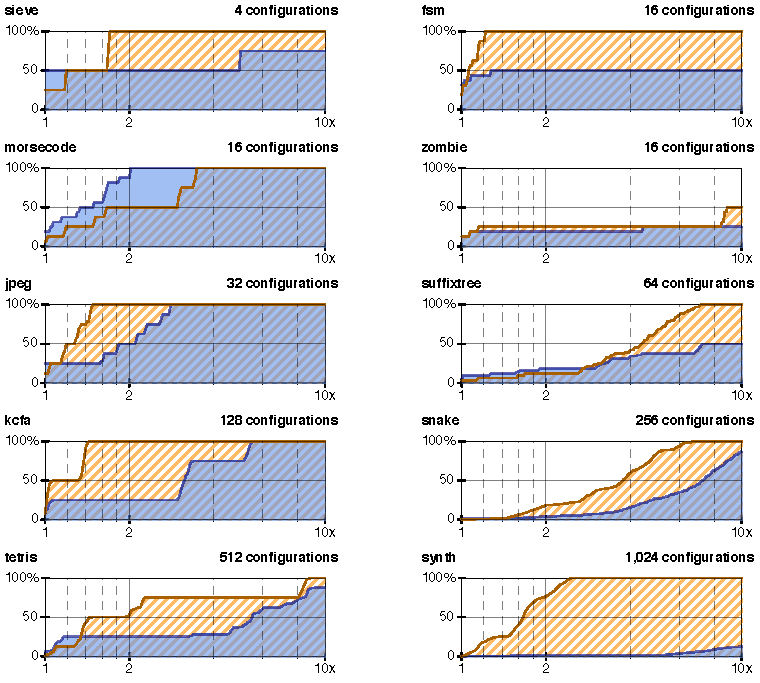
\includegraphics[trim=2.4000000000000004 2.4000000000000004 2.4000000000000004 2.4000000000000004]{pict.pdf}}}\end{FigureInside}\end{Centerfigure}

\Centertext{\Legend{\FigureTarget{\label{t:x28counter_x28x22figurex22_x22figx3aoverheadsx22x29x29}\textsf{Fig.}~\textsf{10}. }{t:x28counter_x28x22figurex22_x22figx3aoverheadsx22x29x29}\textsf{\relax{$\mathsf{TR}\mhyphen\mathsf{\hoshort}$} (blue \raisebox{-0.7999999999999989bp}{\makebox[6.4bp][l]{
\includegraphics[trim=2.4000000000000004 2.4000000000000004 2.4000000000000004 2.4000000000000004]{pict_2.pdf}}}) and \relax{$\mathsf{TR}\mhyphen\mathsf{\foshort}$} (orange \raisebox{-0.7999999999999989bp}{\makebox[6.4bp][l]{
\includegraphics[trim=2.4000000000000004 2.4000000000000004 2.4000000000000004 2.4000000000000004]{pict_3.pdf}}}), each relative to \relax{\eolong} (\relax{$\mathsf{TR}\mhyphen\mathsf{\eoshort}$}).
The \relax{\emph{x}-axis} is log{-}scaled. The unlabeled vertical ticks appear at:
\relax{$1.2$}x, \relax{$1.4$}x, \relax{$1.6$}x, \relax{$1.8$}x, \relax{$4$}x, \relax{$6$}x, and \relax{$8$}x overhead.
A larger area under the curve is better.}}}\end{FigureMulti}

\begin{Figure}\begin{Centerfigure}\begin{FigureInside}\begin{SCentered}\begin{tabular}[t]{@{}r@{}r@{}r@{}r@{}r@{}r@{}r@{}r@{}r@{}r@{}r@{}r@{}r@{}r@{}r@{}r@{}r@{}r@{}r@{}r@{}r@{}}
\hbox{} &
\hbox{\mbox{\hphantom{\Scribtexttt{xx}}}} &
\hbox{\Scribtexttt{sie{\hbox{\texttt{.}}}}} &
\hbox{\mbox{\hphantom{\Scribtexttt{xx}}}} &
\hbox{\Scribtexttt{fsm}} &
\hbox{\mbox{\hphantom{\Scribtexttt{xx}}}} &
\hbox{\Scribtexttt{mor{\hbox{\texttt{.}}}}} &
\hbox{\mbox{\hphantom{\Scribtexttt{xx}}}} &
\hbox{\Scribtexttt{zom{\hbox{\texttt{.}}}}} &
\hbox{\mbox{\hphantom{\Scribtexttt{xx}}}} &
\hbox{\Scribtexttt{jpeg}} &
\hbox{\mbox{\hphantom{\Scribtexttt{xx}}}} &
\hbox{\Scribtexttt{suf{\hbox{\texttt{.}}}}} &
\hbox{\mbox{\hphantom{\Scribtexttt{xx}}}} &
\hbox{\Scribtexttt{kcfa}} &
\hbox{\mbox{\hphantom{\Scribtexttt{xx}}}} &
\hbox{\Scribtexttt{sna{\hbox{\texttt{.}}}}} &
\hbox{\mbox{\hphantom{\Scribtexttt{xx}}}} &
\hbox{\Scribtexttt{tet{\hbox{\texttt{.}}}}} &
\hbox{\mbox{\hphantom{\Scribtexttt{xx}}}} &
\hbox{\Scribtexttt{syn{\hbox{\texttt{.}}}}} \\
\hbox{\relax{$\mathsf{TR}\mhyphen\mathsf{\hoshort}$}} &
\hbox{\mbox{\hphantom{\Scribtexttt{xx}}}} &
\hbox{21.76x} &
\hbox{\mbox{\hphantom{\Scribtexttt{xx}}}} &
\hbox{506.10x} &
\hbox{\mbox{\hphantom{\Scribtexttt{xx}}}} &
\hbox{2.01x} &
\hbox{\mbox{\hphantom{\Scribtexttt{xx}}}} &
\hbox{1072.80x} &
\hbox{\mbox{\hphantom{\Scribtexttt{xx}}}} &
\hbox{2.81x} &
\hbox{\mbox{\hphantom{\Scribtexttt{xx}}}} &
\hbox{24.59x} &
\hbox{\mbox{\hphantom{\Scribtexttt{xx}}}} &
\hbox{5.57x} &
\hbox{\mbox{\hphantom{\Scribtexttt{xx}}}} &
\hbox{13.15x} &
\hbox{\mbox{\hphantom{\Scribtexttt{xx}}}} &
\hbox{13.93x} &
\hbox{\mbox{\hphantom{\Scribtexttt{xx}}}} &
\hbox{51.38x} \\
\hbox{\relax{$\mathsf{TR}\mhyphen\mathsf{\foshort}$}} &
\hbox{\mbox{\hphantom{\Scribtexttt{xx}}}} &
\hbox{1.69x} &
\hbox{\mbox{\hphantom{\Scribtexttt{xx}}}} &
\hbox{1.21x} &
\hbox{\mbox{\hphantom{\Scribtexttt{xx}}}} &
\hbox{3.48x} &
\hbox{\mbox{\hphantom{\Scribtexttt{xx}}}} &
\hbox{20.36x} &
\hbox{\mbox{\hphantom{\Scribtexttt{xx}}}} &
\hbox{1.47x} &
\hbox{\mbox{\hphantom{\Scribtexttt{xx}}}} &
\hbox{7.10x} &
\hbox{\mbox{\hphantom{\Scribtexttt{xx}}}} &
\hbox{1.44x} &
\hbox{\mbox{\hphantom{\Scribtexttt{xx}}}} &
\hbox{6.72x} &
\hbox{\mbox{\hphantom{\Scribtexttt{xx}}}} &
\hbox{8.88x} &
\hbox{\mbox{\hphantom{\Scribtexttt{xx}}}} &
\hbox{2.49x}\end{tabular}\end{SCentered}\end{FigureInside}\end{Centerfigure}

\Centertext{\Legend{\FigureTarget{\label{t:x28counter_x28x22figurex22_x22figx3amaxx2doverheadx22x29x29}\textsf{Fig.}~\textsf{11}. }{t:x28counter_x28x22figurex22_x22figx3amaxx2doverheadx22x29x29}\textsf{Worst{-}case overhead for \relax{\holong} (\relax{$\mathsf{TR}\mhyphen\mathsf{\hoshort}$}) and \relax{\folong} (\relax{$\mathsf{TR}\mhyphen\mathsf{\foshort}$}), each relative to \relax{\eolong}.}}}\end{Figure}

\Ssubsection{Protocol}{Protocol}\label{t:x28part_x22secx3aevaluationx3aprotocolx22x29}

The evaluation reports the performance of the \relax{\holong} (\relax{$\mathsf{TR}\mhyphen\mathsf{\hoshort}$}),
 \relax{\eolong} (\relax{$\mathsf{TR}\mhyphen\mathsf{\eoshort}$}), and \relax{\folong} (\relax{$\mathsf{TR}\mhyphen\mathsf{\foshort}$}) approaches
 on ten Typed Racket programs.
Nine programs are the functional benchmarks from prior work on
 Typed Racket; the
 tenth is adapted from a JPEG library.\NoteBox{\NoteContent{\href{https://docs.racket-lang.org/gtp-benchmarks}{\Scribtexttt{docs{\hbox{\texttt{.}}}racket{-}lang{\hbox{\texttt{.}}}org/gtp{-}benchmarks}}}}

For each configuration of each benchmark, and for both \relax{$\mathsf{TR}\mhyphen\mathsf{\hoshort}$} and \relax{$\mathsf{TR}\mhyphen\mathsf{\foshort}$},
 we collected a sequence of eight running times
 by running the program once to account for JIT warmup and
 then an additional eight times for the actual measurement.
For \relax{$\mathsf{TR}\mhyphen\mathsf{\eoshort}$} we measured one sequence of running times
 because all configurations erase to the same program.

All measurements were collected sequentially using Racket v6.10.1 on an
 unloaded Linux machine with two physical AMD Opteron 6376 processors (a NUMA architecture) and
 128GB RAM.
The CPU cores on each processor ran at 2.30 GHz using the {``}performance{''} CPU governor.

\Ssubsection{Evaluation I: Mixed{-}Typed Programs}{Evaluation I: Mixed{-}Typed Programs}\label{t:x28part_x22Evaluationx5fIx5fx5fMixedx2dTypedx5fProgramsx22x29}

Figure~\hyperref[t:x28counter_x28x22figurex22_x22figx3aoverheadsx22x29x29]{\FigureRef{10}{t:x28counter_x28x22figurex22_x22figx3aoverheadsx22x29x29}} plots
 the overhead of \relax{$\mathsf{TR}\mhyphen\mathsf{\hoshort}$} relative to \relax{\eolong} (blue \raisebox{-0.7999999999999989bp}{\makebox[6.4bp][l]{
\includegraphics[trim=2.4000000000000004 2.4000000000000004 2.4000000000000004 2.4000000000000004]{pict_2.pdf}}})
 and the overhead of \relax{$\mathsf{TR}\mhyphen\mathsf{\foshort}$} relative to \relax{\eolong} (orange \raisebox{-0.7999999999999989bp}{\makebox[6.4bp][l]{
\includegraphics[trim=2.4000000000000004 2.4000000000000004 2.4000000000000004 2.4000000000000004]{pict_3.pdf}}})
 for the ten functional programs.
The lines on each plot give the percent of \relax{$D$}{-}deliverable configurations
 for values of \relax{$D$} between \relax{$1$} to \relax{$10$}.
In other words, a point \relax{$(X, Y)$} on a line for \relax{$\mathsf{TR}\mhyphen\mathsf{\hoshort}$} says that \relax{$Y$}\% of all \relax{$\mathsf{TR}\mhyphen\mathsf{\hoshort}$} configurations
 in this program run at most \relax{$X$} times slower than the same program with all types erased.

Since seven of the ten benchmarks have at least one \relax{$\mathsf{TR}\mhyphen\mathsf{\hoshort}$}
 configuration that falls {``}off the charts{''} with an overhead above 10x,
 figure~\hyperref[t:x28counter_x28x22figurex22_x22figx3amaxx2doverheadx22x29x29]{\FigureRef{11}{t:x28counter_x28x22figurex22_x22figx3amaxx2doverheadx22x29x29}} tabulates the worst{-}case overhead in each benchmark.
According to the table, the \relax{\holong} embedding
 may slow a working program by three orders of magnitude.
The largest slowdowns, in \Scribtexttt{fsm} and \Scribtexttt{zombie}, occur because higher{-}order
 values repeatedly cross type boundaries and accumulate monitors.
The worst{-}case performance of \relax{$\mathsf{TR}\mhyphen\mathsf{\foshort}$}
 is always within two orders of magnitude.

\Ssubsection{Evaluation II: Fully{-}Typed Programs}{Evaluation II: Fully{-}Typed Programs}\label{t:x28part_x22Evaluationx5fIIx5fx5fFullyx2dTypedx5fProgramsx22x29}

\begin{Figure}\begin{Centerfigure}\begin{FigureInside}\raisebox{-0.19999999999998863bp}{\makebox[360.00000000000006bp][l]{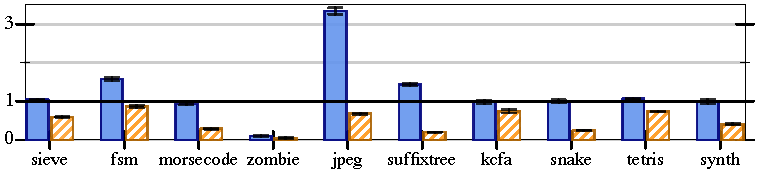
\includegraphics[trim=2.4000000000000004 2.4000000000000004 2.4000000000000004 2.4000000000000004]{pict_4.pdf}}}\end{FigureInside}\end{Centerfigure}

\Centertext{\Legend{\FigureTarget{\label{t:x28counter_x28x22figurex22_x22figx3atypedx2dspeedupx22x29x29}\textsf{Fig.}~\textsf{12}. }{t:x28counter_x28x22figurex22_x22figx3atypedx2dspeedupx22x29x29}\textsf{Speedup of fully{-}typed
\relax{$\mathsf{TR}\mhyphen\mathsf{\hoshort}$} (\raisebox{-0.7999999999999989bp}{\makebox[6.4bp][l]{
\includegraphics[trim=2.4000000000000004 2.4000000000000004 2.4000000000000004 2.4000000000000004]{pict_2.pdf}}})
and \relax{$\mathsf{TR}\mhyphen\mathsf{\foshort}$} (\raisebox{-0.7999999999999989bp}{\makebox[6.4bp][l]{
\includegraphics[trim=2.4000000000000004 2.4000000000000004 2.4000000000000004 2.4000000000000004]{pict_3.pdf}}}),
relative to \relax{$\mathsf{TR}\mhyphen\mathsf{\eoshort}$} (the 1x line).
Taller bars are better than shorter bars.}}}\end{Figure}

The table in figure~\hyperref[t:x28counter_x28x22figurex22_x22figx3atypedx2dspeedupx22x29x29]{\FigureRef{12}{t:x28counter_x28x22figurex22_x22figx3atypedx2dspeedupx22x29x29}} compares the performance
 of fully{-}typed programs (relative to libraries).
The blue bars plot the overhead of \relax{$\mathsf{TR}\mhyphen\mathsf{\hoshort}$} relative to the \relax{\eolong} embedding
 on each benchmark.
The orange bars plot analogous data for \relax{$\mathsf{TR}\mhyphen\mathsf{\foshort}$}
 relative to the \relax{\eolong} embedding.

The \Scribtexttt{jpeg} and \Scribtexttt{zombie} benchmarks are outliers.
In \Scribtexttt{jpeg}, the speedup of \relax{$\mathsf{TR}\mhyphen\mathsf{\hoshort}$} over \relax{\eolong} is high because
 the user program depends on a typed library;\NoteBox{\NoteContent{To be clear, the \relax{$\mathsf{TR}\mhyphen\mathsf{\hoshort}$},
\relax{$\mathsf{TR}\mhyphen\mathsf{\eoshort}$}, and \relax{$\mathsf{TR}\mhyphen\mathsf{\foshort}$} versions of \Scribtexttt{jpeg} rely on the same typed library.
We compile the library using \relax{$\mathsf{TR}\mhyphen\mathsf{\hoshort}$} in all cases because the original library
is from Typed Racket and the original author of \Scribtexttt{jpeg} chose to use this
library.}}
 the library protects itself against \relax{$\mathsf{TR}\mhyphen\mathsf{\eoshort}$} code.
In \Scribtexttt{zombie}, typed code is slower than \relax{\eolong}.
The typed version of \Scribtexttt{zombie} performs a type cast in the inner loop.
The untyped version replaces this cast with a rudimentary predicate check.
This simple change noticeably affects the performance of the fully{-}typed configuration
 (the overhead of monitors, however, dominates the mixed{-}typed configurations).

\Ssubsection{Threats to Validity}{Threats to Validity}\label{t:x28part_x22secx3aevaluationx3athreatsx22x29}

The performance of a full{-}fledged \relax{$\mathsf{TR}\mhyphen\mathsf{\foshort}$} implementation may differ from that
 of our prototype.

On one hand, the prototype is likely to be faster than a full implementation
 because it makes no effort to provide useful error messages.
When a constructor check fails, the prototype simply directs programmers to the
 source location of the check.
Improving these error messages with information about the source of the
 incompatible value is likely to degrade performance in a significant manner.

On the other hand, the performance of a full implementation could improve over
 the prototype in two ways.
First, \relax{$\mathsf{TR}\mhyphen\mathsf{\foshort}$} does not take advantage of the \relax{$\mathsf{TR}\mhyphen\mathsf{\hoshort}$} optimizer
 to remove checks for tag errors.
Integrating the safe parts of the optimizer may offset some cost of the constructor checks.
Second, the completion function for the prototype
 may introduce redundant checks.
For example, consecutive reads from a list suffer the same check
 on the extracted element.

Three other threats are worth noting.
First, \relax{$\mathsf{TR}\mhyphen\mathsf{\foshort}$} does not support Racket{'}s object{-}oriented features\Autobibref{~[\hyperref[t:x28autobib_x22Asumu_Takikawax2c_Daniel_Felteyx2c_Earl_Deanx2c_Robert_Bruce_Findlerx2c_Matthew_Flattx2c_Sam_Tobinx2dHochstadtx2c_and_Matthias_FelleisenTowards_Practical_Gradual_TypingEuropean_Conference_on_Objectx2dOriented_Programmingx2c_ppx2e_4x2dx2d272015x22x29]{\AutobibLink{Takikawa et al\Sendabbrev{.}}} \hyperref[t:x28autobib_x22Asumu_Takikawax2c_Daniel_Felteyx2c_Earl_Deanx2c_Robert_Bruce_Findlerx2c_Matthew_Flattx2c_Sam_Tobinx2dHochstadtx2c_and_Matthias_FelleisenTowards_Practical_Gradual_TypingEuropean_Conference_on_Objectx2dOriented_Programmingx2c_ppx2e_4x2dx2d272015x22x29]{\AutobibLink{2015}}]}.
We expect that scaling the implementation to the full language would not affect the functional benchmarks.
Second, our benchmarks are relatively small; the largest is \Scribtexttt{jpeg} with
 approximately 1,500 lines of code.
Third, the evaluation considers only one fully{-}typed version of each benchmark.
Ascribing different types may affect performance;
 for example, the check for an integer may run faster than the
 check for a natural number.

\sectionNewpage

\Ssection{Implications}{Implications}\label{t:x28part_x22secx3aimplicationsx22x29}

Sections~\ChapRef{\SectionNumberLink{t:x28part_x22secx3adesignx22x29}{2}}{Syntax, Types, and Semantics} and \ChapRef{\SectionNumberLink{t:x28part_x22secx3aevaluationx22x29}{3}}{Performance} present the two critical aspects of the three
approaches to combining statically typed and dynamically typed code via a
twin pair of languages: (1) their semantics within a single framework and
(2) their performance characteristics relative to a single base language on
the same suite of benchmark programs.
Equipped with this objective
information, we can now explain the logical implications and the performance consequences of
choosing one of these three approaches.

For the logical implications, we proceed in a type{-}directed manner.
At the level of base types, there is no difference between the \relax{\holong}
 and \relax{\folong} embeddings, but the \relax{\eolong}
 embedding may give a different result due to a violation of the types (section~\SecRef{\SectionNumberLink{t:x28part_x22subx3abasex22x29}{4.1}}{For Base Types}).
After moving from base types to trees of base types, we can explain
 the truly essential difference between \relax{\holong} and \relax{\folong}:
 while the \relax{\holong} embedding allows
 developers to reason compositionally about type annotations, users of
 the \relax{\folong} variant must always consider the whole program (section~\SecRef{\SectionNumberLink{t:x28part_x22subx3afirstx2dorderx22x29}{4.2}}{For First{-}Order, Non{-}Base Types}).
This non{-}compositional behavior means that a violation of the type annotations
 may go undetected in seemingly type{-}correct code.
Higher{-}order types are similarly afflicted by the non{-}compositional behavior of
 the \relax{\folong} embedding (section~\SecRef{\SectionNumberLink{t:x28part_x22subx3ahox22x29}{4.3}}{For Higher{-}Order Types}).
Lastly, the three approaches provide
 radically different support when it comes to detecting, reporting, and
 debugging boundary errors (section~\SecRef{\SectionNumberLink{t:x28part_x22subx3aerrx22x29}{4.4}}{For Errors and Error Messages}).

For consequences with respect to performance, our work somewhat confirms
the conjectures of the literature that lowering the standards of
safety pays off{---}but only to some degree.
While the \relax{\folong} embedding adds less overhead than the \relax{\holong} embedding to a large portion of the mixed{-}typed
programs (section~\SecRef{\SectionNumberLink{t:x28part_x22subx3aperfx2dmixedx22x29}{4.5}}{For the Performance of Mixed{-}Typed Programs}),
readers must keep two caveats in mind.
For one, the \relax{\folong} approach imposes a run{-}time checking overhead
 that is directly proportional to the number of types in the program.
Second, the \relax{\holong} approach may exploit the full soundness of type annotations.
As a result, programs with many type annotations tend to run faster under
 the \relax{\holong} semantics than the \relax{\folong} one (section~\SecRef{\SectionNumberLink{t:x28part_x22subx3aperfx2dtotalx22x29}{4.6}}{For the Performance of Fully{-}Typed Programs}).

\Ssubsection{For Base Types}{For Base Types}\label{t:x28part_x22subx3abasex22x29}

For a program that computes a value of base type, it can be tempting to think
 that dynamic typing (via \relax{\eolong}) provides all the soundness that matters in practice.
After all, Ruby and Python throw a \Scribtexttt{TypeError} if a program attempts to
 add an integer to a string.

This claim is only true, however, if the static typing system is restricted
 to exactly match the host language{'}s notion of dynamic typing.
Adding a \textit{logical} distinction between natural numbers and integers,
 as demonstrated in the type system of figure~\hyperref[t:x28counter_x28x22figurex22_x22figx3amultix2dpreservationx22x29x29]{\FigureRef{2}{t:x28counter_x28x22figurex22_x22figx3amultix2dpreservationx22x29x29}},
 can lead to silent failures at run{-}time when a negative integer flows into
 a context expecting a natural number.
If the numbers represent votes, for example\Autobibref{~[\hyperref[t:x28autobib_x22Sam_Tobinx2dHochstadtx2c_Matthias_Felleisenx2c_Robert_Bruce_Findlerx2c_Matthew_Flattx2c_Ben_Greenmanx2c_Andrew_Mx2e_Kentx2c_Vincent_Stx2dAmourx2c_Tx2e_Stephen_Stricklandx2c_and_Asumu_TakikawaMigratory_Typingx3a_Ten_years_laterSummit_oN_Advances_in_Programming_Languagesx2c_ppx2e_17x3a1x2dx2d17x3a172017x22x29]{\AutobibLink{Tobin{-}Hochstadt et al\Sendabbrev{.}}} \hyperref[t:x28autobib_x22Sam_Tobinx2dHochstadtx2c_Matthias_Felleisenx2c_Robert_Bruce_Findlerx2c_Matthew_Flattx2c_Ben_Greenmanx2c_Andrew_Mx2e_Kentx2c_Vincent_Stx2dAmourx2c_Tx2e_Stephen_Stricklandx2c_and_Asumu_TakikawaMigratory_Typingx3a_Ten_years_laterSummit_oN_Advances_in_Programming_Languagesx2c_ppx2e_17x3a1x2dx2d17x3a172017x22x29]{\AutobibLink{2017}}]},
 then the lack of run{-}time checking can change the outcome of an election.

Other host languages may allow more diverse kinds of silent failures.
JavaScript, for example, supports adding a number to a string, array, or object.
TypeScript programmers must keep this behavior in mind, and may wish to use
 a library,\NoteBox{\NoteContent{\Scribtexttt{io{\hbox{\texttt{.}}}is} is one such library: \href{https://lorefnon.tech/2018/03/25/typescript-and-validations-at-runtime-boundaries}{\Scribtexttt{lorefnon{\hbox{\texttt{.}}}tech/2018/03/25/typescript{-}and{-}validations{-}at{-}runtime{-}boundaries}}}}
 to protect their type{-}erased code against JavaScript.

Both the \relax{\holong} and \relax{\folong} embeddings are sound for base types, e.g.,
 if \relax{$v$} is a value of type \relax{$\tnat$}, then \relax{$v$} is a natural number.
Informally, both embeddings fully{-}check base types.

\Ssubsection{For First{-}Order, Non{-}Base Types}{For First{-}Order, Non{-}Base Types}\label{t:x28part_x22subx3afirstx2dorderx22x29}

The practical difference between the \relax{\holong} and \relax{\folong} embeddings
 becomes clear in a mixed{-}typed program that deals with pairs.
The \relax{\holong} embedding checks the contents of a pair; the \relax{\folong}
 embedding only checks the constructor:\NoteBox{\NoteContent{In this and similar examples,
we write \relax{$\wellM e : \tau \rrKSstar e'$} to abbreviate:
\relax{$\wellM e : \tau \carrow e'' \mbox{ for some $e''$ and } e'' \rrKSstar e'$}.}}

\relax{$\begin{array}{c l} \\[-2ex]\mbox{\LARGE\checkmark} & \wellM \edyn{(\tpair{\tnat}{\tnat})}{\vpair{-2}{-2}} : \tpair{\tnat}{\tnat} \rrNSstar \boundaryerror\\[1ex]\mbox{\LARGE\danger} & \wellM \edyn{(\tpair{\tnat}{\tnat})}{\vpair{-2}{-2}} : \tpair{\tnat}{\tnat} \rrKSstar \vpair{-2}{-2}\\[1ex] \end{array}$}

\relax{\noindent}Extracting a value from an ill{-}typed pair might not detect the mismatch,
 depending on what type of value the context expects.
For example, a typed context can safely extract a negative integer from a
 pair of natural numbers if the context happens to expect an integer:

\relax{$\begin{array}{c l} \\[-2ex]\mbox{\LARGE\checkmark} & \wellM \efst{(\edyn{(\tpair{\tnat}{\tnat})}{\vpair{-2}{-2}})} : \tnat \rrKSstar \boundaryerror\\[1ex]\mbox{\LARGE\danger} & \wellM \efst{(\edyn{(\tpair{\tnat}{\tnat})}{\vpair{-2}{-2}})} : \arraycell{\tint}{\tnat} \rrKSstar {-2}\\[1ex] \end{array}$}

\relax{\noindent}Similarly, a dynamically{-}typed expression can extract anything
 from a type{-}annotated pair:

\relax{$\begin{array}{c l} \\[-2ex]\mbox{\LARGE\danger} & \wellM \efst{(\esta{(\tpair{\tnat}{\tnat})}{(\edyn{(\tpair{\tnat}{\tnat})}{\vpair{-2}{-2}})})} \rrKDstar -2\\[1ex] \end{array}$}

\relax{\noindent}Put another way, a developer cannot assume
 that a value of type \relax{$\tpair{\tau_0}{\tau_1}$} contains components of type
 \relax{$\tau_0$} and type \relax{$\tau_1$} because type{-}constructor soundness is not compositional.

\begin{Figure}\begin{Centerfigure}\begin{FigureInside}\raisebox{-1.9247395833333485bp}{\makebox[344.00000000000006bp][l]{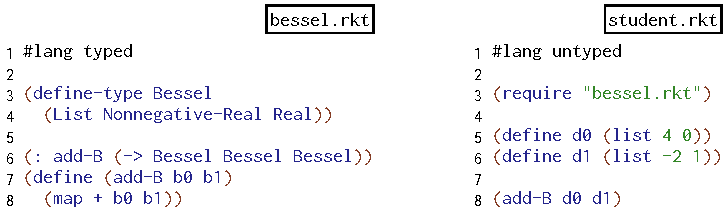
\includegraphics[trim=2.4000000000000004 2.4000000000000004 2.4000000000000004 2.4000000000000004]{pict_5.pdf}}}\end{FigureInside}\end{Centerfigure}

\Centertext{\Legend{\FigureTarget{\label{t:x28counter_x28x22figurex22_x22figx3asilentx2dfailurex22x29x29}\textsf{Fig.}~\textsf{13}. }{t:x28counter_x28x22figurex22_x22figx3asilentx2dfailurex22x29x29}\textsf{Logical error using polar{-}form complex numbers}}}\end{Figure}

Reynolds classic paper on types and abstraction begins with a similar example
 based on a distinction between real numbers and non{-}negative reals\Autobibref{~[\hyperref[t:x28autobib_x22John_Cx2e_ReynoldsTypesx2c_Abstractionx2c_and_Parametric_PolymorphismInformation_Processingx2c_ppx2e_513x2dx2d5231983x22x29]{\AutobibLink{Reynolds}} \hyperref[t:x28autobib_x22John_Cx2e_ReynoldsTypesx2c_Abstractionx2c_and_Parametric_PolymorphismInformation_Processingx2c_ppx2e_513x2dx2d5231983x22x29]{\AutobibLink{1983}}]}:

\begin{SInsetFlow}\textit{In one section, Professor Descartes announced that a complex number was an ordered pair of
reals [...] In the other section, Professor Bessel announced that a complex
number was an ordered pair of reals the first of which was nonnegative [...]}\end{SInsetFlow}

\noindent Figure~\hyperref[t:x28counter_x28x22figurex22_x22figx3asilentx2dfailurex22x29x29]{\FigureRef{13}{t:x28counter_x28x22figurex22_x22figx3asilentx2dfailurex22x29x29}} adapts this example to a mixed{-}typed world.
The typed module on left defines addition for
 {``}Bessel{-}style{''} complex numbers; the function adds the components of the given
 pairs.
The dynamically{-}typed module on the right mistakenly calls the addition function
 on two {``}Descartes{-}style{''} numbers, one of which does not match the type for
 Bessel numbers.

As it turns out, each of the three approaches to migratory typing behaves differently on this program.
The \relax{\holong} embedding correctly rejects the application of \Scribtexttt{add{-}B} at the
 boundary:

\relax{$\begin{array}{c l} \\[-2ex]\mbox{\LARGE\checkmark} & \wellM \texttt{(add-B d0 d1)} \ccNS \boundaryerror\\[1ex] \end{array}$}

\relax{\noindent}The \relax{\eolong} embedding silently computes a well{-}typed, nonsensical result:

\relax{$\begin{array}{c l} \\[-2ex]\mbox{\LARGE\danger} & \wellM \texttt{(add-B d0 d1)} \rrESstar \texttt{(list 2 1)}\\[1ex] \end{array}$}

\relax{\noindent}The \relax{\folong} embedding \textit{either} computes a
 nonsensical result or raises a boundary error somewhere within the \Scribtexttt{map} function:

\relax{$\begin{array}{c l} \\[-2ex]\mbox{\LARGE\danger} & \wellM \texttt{(add-B d0 d1)} \rrKSstar
  \left\{\begin{array}{l l}
     \texttt{(list 2 1)} & \mbox{if \texttt{map} does not check the Bessel type}
  \\ \boundaryerror & \mbox{if \texttt{map} does check the type}
  \end{array}\right.\\[1ex] \end{array}$}

\relax{\noindent}It is impossible to predict the outcome without knowing the
 local type annotations within \Scribtexttt{map}.

\Ssubsection{For Higher{-}Order Types}{For Higher{-}Order Types}\label{t:x28part_x22subx3ahox22x29}

One promising application of migratory typing is to layer a typed interface
 over an existing, dynamically{-}typed library of functions.
For the low effort of converting library documentation into a type specification,
 the library{'}s author and clients benefit from a machine{-}checked API.

Figure~\hyperref[t:x28counter_x28x22figurex22_x22figx3adbx2dappx22x29x29]{\FigureRef{14}{t:x28counter_x28x22figurex22_x22figx3adbx2dappx22x29x29}} demonstrates this use{-}case.
The module on the left represents a dynamically{-}typed library that
 manages a SQL database.
The module on the right represents a dynamically{-}typed web application;
 the application uses the database library to create and access user accounts.
In the middle, the type annotations formalize the interface between the database
 layer and the application.

With the \relax{\holong} embedding, a developer can trust the type annotations.
The database module may assume well{-}typed arguments and the application
 is guaranteed well{-}typed results, despite the lack of static types within
 either module.

In contrast, the \relax{\eolong} embedding completely ignores types at run{-}time
 and treats the middle module of figure~\hyperref[t:x28counter_x28x22figurex22_x22figx3adbx2dappx22x29x29]{\FigureRef{14}{t:x28counter_x28x22figurex22_x22figx3adbx2dappx22x29x29}} as one large comment.
The types are just for documentation and the IDE.

The \relax{\folong} embedding provides a limited compromise: for every
 value that flows from untyped to typed, the implementation checks that the
 value constructor matches the type constructor.
Concretely, there is one run{-}time check that ensures \RktSym{create} is bound to
 a function.

This single check does little to verify the correctness of the dynamically{-}typed
 code.
In terms of the model,
 retrofitting a {``}\relax{\folong}{''} type onto a higher{-}order function \relax{$f$} does not
 enforce that \relax{$f$} respects its arguments:

\relax{$\begin{array}{c l} \\[-2ex]\mbox{\LARGE\danger} & \begin{array}{l}
  f = (\vlam{x}{\eapp{x}{\vpair{1}{1}}})
  \\
  h = \edyn{(\tarr{\tnat}{\tnat})}{(\vlam{y}{\esum{y}{y}})}
  \\
  \wellM \eapp{(\edyn{(\tarr{(\tarr{\tnat}{\tnat})}{\tnat})}{f})}{h} : \tnat \rrKSstar
  \eapp{f}{h} \rrKSstar \eapp{h}{\vpair{1}{1}} \rrKSstar \tagerror
  \\[1ex]
\end{array}\\[1ex] \end{array}$}

\relax{\noindent}Conversely, there is no guarantee that untyped clients of a function \relax{$g$} abide by its interface:

\relax{$\begin{array}{c l} \\[-2ex]\mbox{\LARGE\danger} & \begin{array}{l}
  g = \edyn{(\tarr{\tpair{\tint}{\tint}}{\tint})}{(\vlam{x}{\esnd{x}})}
  \\
  \wellM \eapp{(\esta{(\tarr{\tint}{\tint})}{g})}{{2}} \rrKDstar \esnd{2} \rrKDstar \tagerror
\end{array}\\[1ex] \end{array}$}

\relax{\noindent}Thus the practical benefits of writing a typed API in a
 \relax{\folong} system are vanishingly small.

\begin{Figure}\begin{Centerfigure}\begin{FigureInside}\raisebox{-2.64348958333332bp}{\makebox[380.00000000000006bp][l]{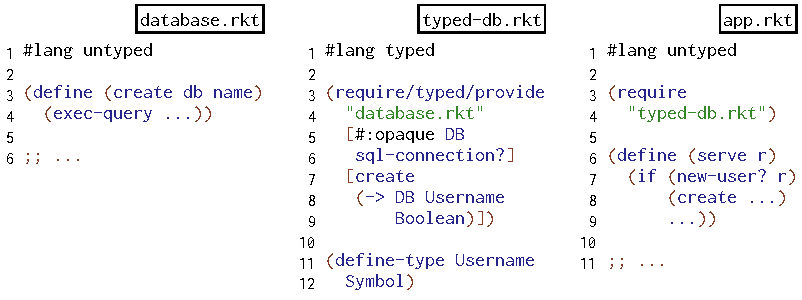
\includegraphics[trim=2.4000000000000004 2.4000000000000004 2.4000000000000004 2.4000000000000004]{pict_6.pdf}}}\end{FigureInside}\end{Centerfigure}

\Centertext{\Legend{\FigureTarget{\label{t:x28counter_x28x22figurex22_x22figx3adbx2dappx22x29x29}\textsf{Fig.}~\textsf{14}. }{t:x28counter_x28x22figurex22_x22figx3adbx2dappx22x29x29}\textsf{Adding types between two untyped modules}}}\end{Figure}

\Ssubsection{For Errors and Error Messages}{For Errors and Error Messages}\label{t:x28part_x22subx3aerrx22x29}

Error messages matter.
As \Autobibref{\hyperref[t:x28autobib_x22Michael_Mx2e_Vitousekx2c_Andrew_Kentx2c_Jeremy_Gx2e_Siekx2c_and_Jim_BakerDesign_and_Evaluation_of_Gradual_Typing_for_PythonDynamic_Languages_Symposiumx2c_ppx2e_45x2dx2d562014x22x29]{\AutobibLink{Vitousek et al\Sendabbrev{.}}}~[\hyperref[t:x28autobib_x22Michael_Mx2e_Vitousekx2c_Andrew_Kentx2c_Jeremy_Gx2e_Siekx2c_and_Jim_BakerDesign_and_Evaluation_of_Gradual_Typing_for_PythonDynamic_Languages_Symposiumx2c_ppx2e_45x2dx2d562014x22x29]{\AutobibLink{2014}}]} claim, improved error messages are {``}one of
 the primary benefits{''} of adding types to a dynamically{-}typed language.
To illustrate, they describe a situation
 in which an untyped module sends a list of strings to a typed function that
 expects a list of numbers:

\begin{SInsetFlow}\textit{if the library authors make use of gradual typing [...] then the error can
be localized and caught before the call to \Scribtexttt{moment} [...] the runtime
error points to the call to \Scribtexttt{moment}}\end{SInsetFlow}

\relax{\noindent}This claim assumes, of course, that the gradual typing system enforces types.

Figure~\hyperref[t:x28counter_x28x22figurex22_x22figx3alistx2derrorx22x29x29]{\FigureRef{15}{t:x28counter_x28x22figurex22_x22figx3alistx2derrorx22x29x29}} turns their illustration into a concrete
 example.
The \Scribtexttt{stats} module computes the \RktSym{m}{-}th \Scribtexttt{moment} of a list of floats;
 it defers most of the computation to the language{'}s list package, meaning
 a call to \Scribtexttt{moment} may cause another boundary{-}crossing.
The \Scribtexttt{client} module calls \Scribtexttt{moment} with an inappropriate list.

The \relax{\holong} embedding catches the error before the
 call to \Scribtexttt{moment}:

\relax{$\begin{array}{c l} \\[-2ex]\mbox{\LARGE\checkmark} & \wellM \texttt{(moment lst 2)} \rrNDstar \texttt{(moment ($\vfromdynN$(Listof(Float), lst)) 2)} \rrNDstar \boundaryerror\\[1ex] \end{array}$}

The \relax{\eolong} embedding performs the call to \Scribtexttt{moment} just like a dynamically{-}typed language would.
If the numeric operations check their inputs, the execution ends in a tag error.
If the primitives are un{-}checked, however, then the call may compute a nonsensical result:

\relax{$\begin{array}{c l} \\[-2ex]\mbox{\LARGE\danger} & \wellM \texttt{(moment lst 2)} \rrEDstar
  \left\{\begin{array}{l l}
     \tagerror & \mbox{if \texttt{mean} or \texttt{-} check for strings}
  \\ -42       & \mbox{if the primitives are unchecked}
  \end{array}\right.\\[1ex] \end{array}$}

The \relax{\folong} embedding confirms that \Scribtexttt{lst} is a list and then proceeds
 with the call.
Since the body of \Scribtexttt{moment} never directly extracts a float from the list,
 it is impossible to predict what happens during the call.
For example, \Scribtexttt{mean} can raise a boundary error, raise a tag error, or
 silently compute a sum of string pointers:

\relax{$\begin{array}{c l} \\[-2ex]\mbox{\LARGE\danger} & \wellM \texttt{(moment lst 2)} \rrKDstar
  \left\{\begin{array}{l l}
     \boundaryerror & \mbox{if \texttt{mean}, \texttt{-}, or \texttt{map} use the @tt{Float} type}
  \\ \tagerror & \mbox{if \texttt{mean} or \texttt{-} check for strings}
  \\ -42       & \mbox{if the primitives are unchecked}
  \end{array}\right.\\[1ex] \end{array}$}

\relax{\noindent}In the case of a boundary error, it is not clear how a first{-}order embedding
 can pinpoint the boundary that is violated.
\Autobibref{\hyperref[t:x28autobib_x22Michael_Mx2e_Vitousekx2c_Cameron_Swordsx2c_and_Jeremy_Gx2e_SiekBig_Types_in_Little_Runtimex3a_Openx2dWorld_Soundness_and_Collaborative_Blame_for_Gradual_Type_SystemsSymposium_on_Principles_of_Programming_Languagesx2c_ppx2e_762x2dx2d7742017x22x29]{\AutobibLink{Vitousek et al\Sendabbrev{.}}}~[\hyperref[t:x28autobib_x22Michael_Mx2e_Vitousekx2c_Cameron_Swordsx2c_and_Jeremy_Gx2e_SiekBig_Types_in_Little_Runtimex3a_Openx2dWorld_Soundness_and_Collaborative_Blame_for_Gradual_Type_SystemsSymposium_on_Principles_of_Programming_Languagesx2c_ppx2e_762x2dx2d7742017x22x29]{\AutobibLink{2017}}]} propose a strategy that points the \relax{\folong}
 error message to the call to \Scribtexttt{moment}, but the strategy may double the
 running time of a program and reports a set of potentially{-}guilty boundaries
 rather than pinpointing the faulty one.

By contrast, the \relax{\holong} embedding can identify the first violation of the
 types by storing debugging information
 in monitor values\Autobibref{~[\hyperref[t:x28autobib_x22Sam_Tobinx2dHochstadtx2c_Matthias_Felleisenx2c_Robert_Bruce_Findlerx2c_Matthew_Flattx2c_Ben_Greenmanx2c_Andrew_Mx2e_Kentx2c_Vincent_Stx2dAmourx2c_Tx2e_Stephen_Stricklandx2c_and_Asumu_TakikawaMigratory_Typingx3a_Ten_years_laterSummit_oN_Advances_in_Programming_Languagesx2c_ppx2e_17x3a1x2dx2d17x3a172017x22x29]{\AutobibLink{Tobin{-}Hochstadt et al\Sendabbrev{.}}} \hyperref[t:x28autobib_x22Sam_Tobinx2dHochstadtx2c_Matthias_Felleisenx2c_Robert_Bruce_Findlerx2c_Matthew_Flattx2c_Ben_Greenmanx2c_Andrew_Mx2e_Kentx2c_Vincent_Stx2dAmourx2c_Tx2e_Stephen_Stricklandx2c_and_Asumu_TakikawaMigratory_Typingx3a_Ten_years_laterSummit_oN_Advances_in_Programming_Languagesx2c_ppx2e_17x3a1x2dx2d17x3a172017x22x29]{\AutobibLink{2017}}]}.
With the relevant boundary term, the developer knows exactly where to
 begin debugging: either the type annotation is wrong or the dynamically{-}typed
 code does not match the type.

Generally speaking,
 \relax{\holong} discovers more errors than \relax{\folong} and
 \relax{\folong} discovers more errors than \relax{\eolong}:

\begin{Figure}\begin{Centerfigure}\begin{FigureInside}\raisebox{-2.12890625bp}{\makebox[358.4000000000001bp][l]{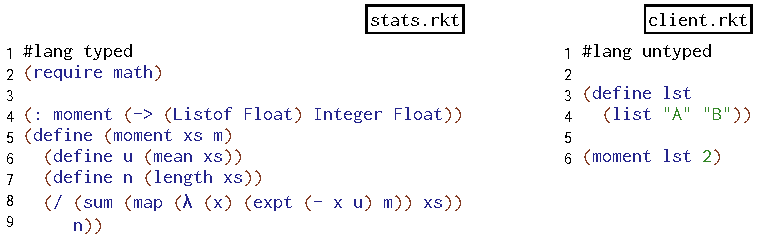
\includegraphics[trim=2.4000000000000004 2.4000000000000004 2.4000000000000004 2.4000000000000004]{pict_7.pdf}}}\end{FigureInside}\end{Centerfigure}

\Centertext{\Legend{\FigureTarget{\label{t:x28counter_x28x22figurex22_x22figx3alistx2derrorx22x29x29}\textsf{Fig.}~\textsf{15}. }{t:x28counter_x28x22figurex22_x22figx3alistx2derrorx22x29x29}\textsf{Type{-}mismatch between a library function and client, adapted from \Autobibref{\hyperref[t:x28autobib_x22Michael_Mx2e_Vitousekx2c_Andrew_Kentx2c_Jeremy_Gx2e_Siekx2c_and_Jim_BakerDesign_and_Evaluation_of_Gradual_Typing_for_PythonDynamic_Languages_Symposiumx2c_ppx2e_45x2dx2d562014x22x29]{\AutobibLink{Vitousek et al\Sendabbrev{.}}}~[\hyperref[t:x28autobib_x22Michael_Mx2e_Vitousekx2c_Andrew_Kentx2c_Jeremy_Gx2e_Siekx2c_and_Jim_BakerDesign_and_Evaluation_of_Gradual_Typing_for_PythonDynamic_Languages_Symposiumx2c_ppx2e_45x2dx2d562014x22x29]{\AutobibLink{2014}}]}.}}}\end{Figure}

\begin{Subflow}\relax{\vspace{0.4ex}}
\textbf{Theorem 2.9} : \label{t:x28tech_x22error_simulationx22x29}\textit{\relax{$\eerr$} approximation}
\relax{\\[-1.8ex]}

\noindent \begin{bigtabular}{@{\bigtableleftpad}@{\SBoxedLeft}l@{}}
\begin{minipage}[c]{1.0\linewidth}
\begin{Subflow}If \relax{$e \in \exprsta$} and \relax{$\wellM e : \tau$} then the following statements hold:


\noindent \begin{itemize}\atItemizeStart

\item if \relax{$e \rrESstar \eerr$} then \relax{$e \rrKSstar \eerr$}

\item if \relax{$e \rrKSstar \eerr$} then \relax{$e \rrNSstar \eerr$}\end{itemize}\end{Subflow} \end{minipage}
\end{bigtabular}\end{Subflow}

\noindent \begin{Subflow}\textit{Proof (sketch)}: Informally, each pair of reduction relations is {``}equivalent{''} up to their strategies
 for enforcing static types.
The supplement defines these equivalences as simulation relations\Autobibref{~[\hyperref[t:x28autobib_x22Ben_Greenman_and_Matthias_FelleisenA_Spectrum_of_Type_Soundness_and_Performance_Supplementary_MaterialNortheastern_Universityx2c_NUx2dCCISx2d2018x2d0022018x22x29]{\AutobibLink{Greenman and Felleisen}} \hyperref[t:x28autobib_x22Ben_Greenman_and_Matthias_FelleisenA_Spectrum_of_Type_Soundness_and_Performance_Supplementary_MaterialNortheastern_Universityx2c_NUx2dCCISx2d2018x2d0022018x22x29]{\AutobibLink{2018}}]}.\relax{$\hfill\qedsymbol$}\end{Subflow}

The reverse implications do not hold.
As section~\SecRef{\SectionNumberLink{t:x28part_x22subx3abasex22x29}{4.1}}{For Base Types} explains, the expression \relax{$(\edyn{\tnat}{{-2}})$}
 steps to a boundary error via \relax{$\rrKSstar$} but not via the \relax{$\rrESstar$} relation.
Section~\SecRef{\SectionNumberLink{t:x28part_x22subx3afirstx2dorderx22x29}{4.2}}{For First{-}Order, Non{-}Base Types} presents an example where \relax{$\rrNSstar$} steps
 a boundary error and \relax{$\rrKSstar$} produces a value.

\Ssubsection{For the Performance of Mixed{-}Typed Programs}{For the Performance of Mixed{-}Typed Programs}\label{t:x28part_x22subx3aperfx2dmixedx22x29}

Enforcing soundness in a mixed{-}typed program adds performance overhead.
As the graphs in section~\ChapRef{\SectionNumberLink{t:x28part_x22secx3aevaluationx22x29}{3}}{Performance} demonstrate,
 this cost can be high (10x) in the \relax{\folong} embedding and enormous
 (1000x) in the \relax{\holong} embedding.

The \relax{\folong} embedding incurs type{-}constructor checks at three places:
 type boundaries, applications of typed functions, and explicit \relax{$\vchk$} terms.
While each check adds a small cost,\NoteBox{\NoteContent{In the model, checks have \relax{$O(1)$} cost.
In the implementation, checks have near{-}constant cost \relax{$O(n)$} where
\relax{$n$} is the number of types in the widest union type
\relax{$(\tau_0 \cup \ldots \cup \tau_{n-1})$} in the program.}}
 these costs accumulate.
The added code and branches may affect JIT compilation.

The \relax{\holong} embedding incurs three significant kinds of costs.
First, there is the cost of checking a value at a boundary.
Second, there is an allocation cost when a higher{-}order value crosses a boundary.
Third, monitored values suffer an indirection cost; for example,
 a monitor guarding a dynamically{-}typed function must check every result computed
 by the function.

Each kind of cost may be arbitrarily large.
The (time) cost of checking an algebraic type depends on the size of the
 given value.
The (time and space) cost of allocation grows with the number
 of boundary{-}crossings, as does the (time) cost of indirection.
In the following example, an untyped function crosses three boundaries and
 consequently accumulates three monitors:

\relax{$\begin{array}{c l} \\[-2ex]\mbox{\LARGE\danger} & \begin{array}{l}
  \edyn{(\tarr{\tnat}{\tnat})}{(\esta{(\tarr{\tint}{\tint})}{(\edyn{(\tarr{\tint}{\tint})}{\vlam{x}{x}})})}
  \\ \rrNSstar \vmonfun{(\tarr{\tnat}{\tnat})}{(\vmonfun{(\tarr{\tint}{\tint})}{(\vmonfun{(\tarr{\tint}{\tint})}{\vlam{x}{x}})})}
  \\[0.4ex]
\end{array}\\[1ex] \end{array}$}

\relax{\noindent}Finally, the indirection added by monitors may limit the effectiveness of
 a JIT compiler.

\Ssubsection{For the Performance of Fully{-}Typed Programs}{For the Performance of Fully{-}Typed Programs}\label{t:x28part_x22subx3aperfx2dtotalx22x29}

If a program has few dynamically{-}typed components, then the \relax{\folong}
 embedding is likely to perform the worst of the three embeddings.
This poor performance comes about because all typed expressions unconditionally
 check their inputs.
For example, a function that adds both elements of a pair value must check
 that its input has integer{-}valued components:

\relax{$\begin{array}{c l} \\[-2ex]\mbox{\LARGE\danger} & \begin{array}{l}
\wellM \vlam{\tann{x}{\tpair{\tint}{\tint}}}{\esum{(\efst{x})}{(\esnd{x})}} : \tarr{\tpair{\tint}{\tint}}{\tint}
\\ \carrow \vlam{\tann{x}{\tpair{\tint}{\tint}}}{\esum{(\echk{\tint}{(\efst{x})})}{(\echk{\tint}{(\esnd{x})})}}
\\[0.4ex]
\end{array}\\[1ex] \end{array}$}

\relax{\noindent}As a rule{-}of{-}thumb, adding types imposes (at least) a linear{-}time performance
 degredation\Autobibref{~[\hyperref[t:x28autobib_x22Ben_Greenman_and_Matthias_FelleisenA_Spectrum_of_Type_Soundness_and_Performance_Supplementary_MaterialNortheastern_Universityx2c_NUx2dCCISx2d2018x2d0022018x22x29]{\AutobibLink{Greenman and Felleisen}} \hyperref[t:x28autobib_x22Ben_Greenman_and_Matthias_FelleisenA_Spectrum_of_Type_Soundness_and_Performance_Supplementary_MaterialNortheastern_Universityx2c_NUx2dCCISx2d2018x2d0022018x22x29]{\AutobibLink{2018}}; \hyperref[t:x28autobib_x22Ben_Greenman_and_Zeina_MigeedOn_the_Cost_of_Typex2dTag_SoundnessWorkshop_on_Partial_Evaluation_and_Program_Manipulationx2c_ppx2e_30x2dx2d392018x22x29]{\AutobibLink{Greenman and Migeed}} \hyperref[t:x28autobib_x22Ben_Greenman_and_Zeina_MigeedOn_the_Cost_of_Typex2dTag_SoundnessWorkshop_on_Partial_Evaluation_and_Program_Manipulationx2c_ppx2e_30x2dx2d392018x22x29]{\AutobibLink{2018}}]}.

The \relax{\holong} embedding pays to enforce soundness only if static
 and dynamic components interact.
If there are few interactions, the program spends little time enforcing soundness.

Furthermore, the soundness of the \relax{\holong} embedding means that a compiler can
 apply classic, type{-}directed optimizations.
Thus the \relax{\holong} embedding{'}s performance can exceed that of the \relax{\eolong} embedding, as shown in figure~\hyperref[t:x28counter_x28x22figurex22_x22figx3atypedx2dspeedupx22x29x29]{\FigureRef{12}{t:x28counter_x28x22figurex22_x22figx3atypedx2dspeedupx22x29x29}}.
Typed Racket (\relax{$\mathsf{TR}\mhyphen\mathsf{\hoshort}$}) in particular applies optimizations to unbox primitive values,
 select low{-}level primitive operations,
 provide fast access to data structures,
 and eliminate unused branches\Autobibref{~[\hyperref[t:x28autobib_x22Vincent_Stx2dAmourx2c_Sam_Tobinx2dHochstadtx2c_and_Matthias_FelleisenOptimization_coachingConference_on_Objectx2dOriented_Programmingx2c_Systemsx2c_Languages_and_Applicationsx2c_ppx2e_163x2dx2d1782012x22x29]{\AutobibLink{St{-}Amour et al\Sendabbrev{.}}} \hyperref[t:x28autobib_x22Vincent_Stx2dAmourx2c_Sam_Tobinx2dHochstadtx2c_and_Matthias_FelleisenOptimization_coachingConference_on_Objectx2dOriented_Programmingx2c_Systemsx2c_Languages_and_Applicationsx2c_ppx2e_163x2dx2d1782012x22x29]{\AutobibLink{2012\AutobibLink{a}}}; \hyperref[t:x28autobib_x22Vincent_Stx2dAmourx2c_Sam_Tobinx2dHochstadtx2c_Matthew_Flattx2c_and_Matthias_FelleisenTyping_the_Numeric_TowerSymposium_on_Practical_Aspects_of_Declarative_Languagesx2c_ppx2e_289x2dx2d3032012x22x29]{\AutobibLink{St{-}Amour et al\Sendabbrev{.}}} \hyperref[t:x28autobib_x22Vincent_Stx2dAmourx2c_Sam_Tobinx2dHochstadtx2c_Matthew_Flattx2c_and_Matthias_FelleisenTyping_the_Numeric_TowerSymposium_on_Practical_Aspects_of_Declarative_Languagesx2c_ppx2e_289x2dx2d3032012x22x29]{\AutobibLink{2012\AutobibLink{b}}}]}.

\sectionNewpage

\Ssection{Existing Systems}{Existing Systems}\label{t:x28part_x22secx3aexistingx2dsystemsx22x29}

Figure~\hyperref[t:x28counter_x28x22figurex22_x22figx3aexistingx2dsystemsx22x29x29]{\FigureRef{16}{t:x28counter_x28x22figurex22_x22figx3aexistingx2dsystemsx22x29x29}} classifies existing migratory and mixed{-}typed
 systems in terms of the three approaches.\NoteBox{\NoteContent{The interested reader may
wish to consult the supplement, in which we instantiate
the framework of section~\ChapRef{\SectionNumberLink{t:x28part_x22secx3adesignx22x29}{2}}{Syntax, Types, and Semantics} for several existing systems\Autobibref{~[\hyperref[t:x28autobib_x22Ben_Greenman_and_Matthias_FelleisenA_Spectrum_of_Type_Soundness_and_Performance_Supplementary_MaterialNortheastern_Universityx2c_NUx2dCCISx2d2018x2d0022018x22x29]{\AutobibLink{Greenman and Felleisen}} \hyperref[t:x28autobib_x22Ben_Greenman_and_Matthias_FelleisenA_Spectrum_of_Type_Soundness_and_Performance_Supplementary_MaterialNortheastern_Universityx2c_NUx2dCCISx2d2018x2d0022018x22x29]{\AutobibLink{2018}}]}.
The supplement also has URLs for the languages.}}
Systems listed under the box labeled \textit{\relax{\holong} embedding} enforce
 higher{-}order types at run{-}time.
Systems under the \textit{\relax{\eolong} embedding} label provide an optional static type checker
 but do not use types to determine program behavior.
Systems under the \textit{\relax{\folong} embedding} label enforce type boundaries
 with some form of first{-}order checks {---} the details vary between systems.
In Dart 2 and Nom,
 every structured value is associated with run{-}time type
 information (e.g., the value is an object and is associated with a class name);
 the boundary checks perform a subtype test using this type information.
SafeTS is similar, however, the type information is structural rather than
 nominal and may gain new fields (but not methods) by crossing a boundary.
Reticulated and our \relax{$\mathsf{TR}\mhyphen\mathsf{\foshort}$} prototype perform first{-}order checks similar
 to those outlined in section~\SecRef{\SectionNumberLink{t:x28part_x22secx3alocallyx2ddefensivex2dembeddingx22x29}{2.5}}{\relax{\FOlong} Embedding} and
 furthermore rewrite statically{-}typed code to protect against untyped
 values.

Several systems are located on dashed lines in figure~\hyperref[t:x28counter_x28x22figurex22_x22figx3aexistingx2dsystemsx22x29x29]{\FigureRef{16}{t:x28counter_x28x22figurex22_x22figx3aexistingx2dsystemsx22x29x29}}
 because they compromise between two approaches.
StrongScript and Thorn include two kinds of types: concrete types and like types.
Both types are checked statically, but only concrete types are enforced at
 run{-}time.
In other words, a program that uses only like types has \relax{\eolong} behavior.
These two related systems are on different lines because only StrongScript supports
 higher{-}order types (such types must be concrete).

Pyret falls between the \relax{\folong} and \relax{\eolong} approaches.
If a program contains type annotations, then Pyret enforces each annotation
 with a run{-}time type constructor check.
A programmer can therefore opt into type{-}constructor
 soundness through disciplined use of type annotations.

\begin{Figure}\begin{Centerfigure}\begin{FigureInside}\relax{\begin{tikzpicture}
  \def\embeddingskip{4cm}
  \node (N)
    [draw,align=center]
    {\textbf{\relax{\HOlong} Embedding}};
  \node (Nsub)
    [align=center,below of=N,yshift=1ex]
    {Gradualtalk\relax{$^{\dagger}\!$}, \\
     TPD\relax{$^{\dagger}\!$}, Typed Racket\relax{$^{\dagger}\!$}};

  \node (NE)
    [align=center,below of=N,xshift=\embeddingskip]
    {StrongScript};

  \node (E)
    [draw,align=center,below of=NE,xshift=\embeddingskip]
    {\textbf{\relax{\EOlong} Embedding}};
  \node (Esub)
    [align=center,below of=E,yshift=-3ex]
    {ActionScript\relax{$^{\dagger}\!$}, mypy\relax{$^{\dagger}\!$}, \\
     Flow\relax{$^{\dagger}\!$}, Hack\relax{$^{\dagger}\!$}, Pyre\relax{$^{\dagger}\!$}, Pytype\relax{$^{\dagger}\!$}, \\
     rtc\relax{$^{\dagger}\!$}, Strongtalk\relax{$^{\dagger}\!$}, \\
     TypeScript\relax{$^{\dagger}\!$}, Typed Clojure\relax{$^{\dagger}\!$}, \\
     Typed Lua\relax{$^{\dagger}\!$}};

  \node (ELD)
    [align=center,below of=E,xshift=-\embeddingskip]
    {Pyret\relax{$^{\dagger}\!$}, \\
     Thorn};

  \node (LD)
    [draw,align=center,below of=ELD,xshift=-\embeddingskip]
    {\textbf{\relax{\FOlong} Embedding}};
  \node (LDsub)
    [align=center,below of=LD,yshift=1ex]
    {Dart 2, Nom, Reticulated\relax{$^{\dagger}\!$}, \\
     SafeTS, \relax{$\mathsf{TR}\mhyphen\mathsf{\foshort}$}\relax{$^{\dagger}\!$} (section \ChapRef{\SectionNumberLink{t:x28part_x22secx3aevaluationx22x29}{3}}{Performance})};

  \node (legend)
    [align=right,right of=E,yshift=-20ex]
    {($\dagger$ : migratory typing system)};

  \draw[-,dashed] (N) -- (NE);
  \draw[-,dashed] (NE) -- (E);
  \draw[-,dashed] (LD) -- (ELD);
  \draw[-,dashed] (ELD) -- (E);
\end{tikzpicture}}\end{FigureInside}\end{Centerfigure}

\Centertext{\Legend{\FigureTarget{\label{t:x28counter_x28x22figurex22_x22figx3aexistingx2dsystemsx22x29x29}\textsf{Fig.}~\textsf{16}. }{t:x28counter_x28x22figurex22_x22figx3aexistingx2dsystemsx22x29x29}\textsf{Design space of migratory and mixed{-}typed systems.}}}\end{Figure}

\sectionNewpage

\Ssection{Related Work}{Related Work}\label{t:x28part_x22secx3arelatedx2dworkx22x29}

The idea of equipping a dynamically typed language with static type information
 goes back at least to the compiler hints in MACLISP\Autobibref{~[\hyperref[t:x28autobib_x22David_Ax2e_MoonMACLISP_Reference_ManualMITx2c_Revision_01974x22x29]{\AutobibLink{Moon}} \hyperref[t:x28autobib_x22David_Ax2e_MoonMACLISP_Reference_ManualMITx2c_Revision_01974x22x29]{\AutobibLink{1974}}]}.
Early work focused on type reconstruction for dynamically{-}typed
 programs\Autobibref{~[\hyperref[t:x28autobib_x22Christopher_Andersonx2c_Paola_Gianninix2c_and_Sophia_DrossopoulouTowards_Type_Inference_for_JavaScriptEuropean_Conference_on_Objectx2dOriented_Programmingx2c_ppx2e_428x2dx2d4522005x22x29]{\AutobibLink{Anderson et al\Sendabbrev{.}}} \hyperref[t:x28autobib_x22Christopher_Andersonx2c_Paola_Gianninix2c_and_Sophia_DrossopoulouTowards_Type_Inference_for_JavaScriptEuropean_Conference_on_Objectx2dOriented_Programmingx2c_ppx2e_428x2dx2d4522005x22x29]{\AutobibLink{2005}}; \hyperref[t:x28autobib_x22Norihisa_SuzukiInferring_Types_in_SmalltalkSymposium_on_Principles_of_Programming_Languagesx2c_ppx2e_187x2dx2d1991981x22x29]{\AutobibLink{Suzuki}} \hyperref[t:x28autobib_x22Norihisa_SuzukiInferring_Types_in_SmalltalkSymposium_on_Principles_of_Programming_Languagesx2c_ppx2e_187x2dx2d1991981x22x29]{\AutobibLink{1981}}; \hyperref[t:x28autobib_x22Andrew_Kx2e_Wright_and_Robert_CartwrightA_Practical_Soft_Type_System_for_SchemeTransactions_on_Programming_Languages_and_Systems_19x281x29x2c_ppx2e_87x2dx2d1521997x22x29]{\AutobibLink{Wright and Cartwright}} \hyperref[t:x28autobib_x22Andrew_Kx2e_Wright_and_Robert_CartwrightA_Practical_Soft_Type_System_for_SchemeTransactions_on_Programming_Languages_and_Systems_19x281x29x2c_ppx2e_87x2dx2d1521997x22x29]{\AutobibLink{1997}}]}.
Over the past decade, researchers turned to the problem of creating a
 multi{-}language system\Autobibref{~[\hyperref[t:x28autobib_x22Kathryn_Ex2e_Grayx2c_Robert_Bruce_Findlerx2c_and_Matthew_FlattFinex2dGrained_Interoperability_Through_Mirrors_and_ContractsConference_on_Objectx2dOriented_Programmingx2c_Systemsx2c_Languages_and_Applicationsx2c_ppx2e_231x2dx2d2452005x22x29]{\AutobibLink{Gray et al\Sendabbrev{.}}} \hyperref[t:x28autobib_x22Kathryn_Ex2e_Grayx2c_Robert_Bruce_Findlerx2c_and_Matthew_FlattFinex2dGrained_Interoperability_Through_Mirrors_and_ContractsConference_on_Objectx2dOriented_Programmingx2c_Systemsx2c_Languages_and_Applicationsx2c_ppx2e_231x2dx2d2452005x22x29]{\AutobibLink{2005}}]}
 that provides a type soundness guarantee\Autobibref{~[\hyperref[t:x28autobib_x22Kenneth_Knowles_and_Cormac_FlanaganHybrid_Type_CheckingTransactions_on_Programming_Languages_and_Systems_32x286x29x2c_ppx2e_1x2dx2d342010x22x29]{\AutobibLink{Knowles and Flanagan}} \hyperref[t:x28autobib_x22Kenneth_Knowles_and_Cormac_FlanaganHybrid_Type_CheckingTransactions_on_Programming_Languages_and_Systems_32x286x29x2c_ppx2e_1x2dx2d342010x22x29]{\AutobibLink{2010}}; \hyperref[t:x28autobib_x22Jacob_Matthews_and_Robert_Bruce_FindlerOperational_Semantics_for_Multix2dlanguage_ProgramsTransactions_on_Programming_Languages_and_Systems_31x283x29x2c_ppx2e_1x2dx2d442009x22x29]{\AutobibLink{Matthews and Findler}} \hyperref[t:x28autobib_x22Jacob_Matthews_and_Robert_Bruce_FindlerOperational_Semantics_for_Multix2dlanguage_ProgramsTransactions_on_Programming_Languages_and_Systems_31x283x29x2c_ppx2e_1x2dx2d442009x22x29]{\AutobibLink{2009}}; \hyperref[t:x28autobib_x22Jeremy_Gx2e_Siek_and_Walid_TahaGradual_Typing_for_Functional_LanguagesScheme_and_Functional_Programmingx2e_University_of_Chicagox2c_TRx2d2006x2d062006x22x29]{\AutobibLink{Siek and Taha}} \hyperref[t:x28autobib_x22Jeremy_Gx2e_Siek_and_Walid_TahaGradual_Typing_for_Functional_LanguagesScheme_and_Functional_Programmingx2e_University_of_Chicagox2c_TRx2d2006x2d062006x22x29]{\AutobibLink{2006}}; \hyperref[t:x28autobib_x22Sam_Tobinx2dHochstadt_and_Matthias_FelleisenInterlanguage_Migrationx3a_from_Scripts_to_ProgramsDynamic_Languages_Symposiumx2c_ppx2e_964x2dx2d9742006x22x29]{\AutobibLink{Tobin{-}Hochstadt and Felleisen}} \hyperref[t:x28autobib_x22Sam_Tobinx2dHochstadt_and_Matthias_FelleisenInterlanguage_Migrationx3a_from_Scripts_to_ProgramsDynamic_Languages_Symposiumx2c_ppx2e_964x2dx2d9742006x22x29]{\AutobibLink{2006}}]}.

\Ssubsection{Gradual Typing}{Gradual Typing}\label{t:x28part_x22Gradualx5fTypingx22x29}

Migratory typing is closely related to gradual typing\Autobibref{~[\hyperref[t:x28autobib_x22Jeremy_Gx2e_Siek_and_Walid_TahaGradual_Typing_for_Functional_LanguagesScheme_and_Functional_Programmingx2e_University_of_Chicagox2c_TRx2d2006x2d062006x22x29]{\AutobibLink{Siek and Taha}} \hyperref[t:x28autobib_x22Jeremy_Gx2e_Siek_and_Walid_TahaGradual_Typing_for_Functional_LanguagesScheme_and_Functional_Programmingx2e_University_of_Chicagox2c_TRx2d2006x2d062006x22x29]{\AutobibLink{2006}}; \hyperref[t:x28autobib_x22Jeremy_Gx2e_Siekx2c_Michael_Mx2e_Vitousekx2c_Matteo_Ciminix2c_and_John_Tang_BoylandRefined_Criteria_for_Gradual_TypingSummit_oN_Advances_in_Programming_Languagesx2c_ppx2e_274x2dx2d2932015x22x29]{\AutobibLink{Siek et al\Sendabbrev{.}}} \hyperref[t:x28autobib_x22Jeremy_Gx2e_Siekx2c_Michael_Mx2e_Vitousekx2c_Matteo_Ciminix2c_and_John_Tang_BoylandRefined_Criteria_for_Gradual_TypingSummit_oN_Advances_in_Programming_Languagesx2c_ppx2e_274x2dx2d2932015x22x29]{\AutobibLink{2015}}]}.
In the broad sense, the term gradual typing has come to describe
 any type system that allows some amount of dynamic typing.
In the precise sense of \Autobibref{\hyperref[t:x28autobib_x22Jeremy_Gx2e_Siekx2c_Michael_Mx2e_Vitousekx2c_Matteo_Ciminix2c_and_John_Tang_BoylandRefined_Criteria_for_Gradual_TypingSummit_oN_Advances_in_Programming_Languagesx2c_ppx2e_274x2dx2d2932015x22x29]{\AutobibLink{Siek et al\Sendabbrev{.}}}~[\hyperref[t:x28autobib_x22Jeremy_Gx2e_Siekx2c_Michael_Mx2e_Vitousekx2c_Matteo_Ciminix2c_and_John_Tang_BoylandRefined_Criteria_for_Gradual_TypingSummit_oN_Advances_in_Programming_Languagesx2c_ppx2e_274x2dx2d2932015x22x29]{\AutobibLink{2015}}]}, a gradual typing
 system includes: (1) a dynamic type that may be implicitly cast to
 any other type; (2) a relation between types that are equal up to occurrences
 of the dynamic type; and (3) a proof that replacing any
 type with the dynamic type can only (3a) remove a compile{-}time type error
 or (3b) remove a boundary error.

Gradual typing and migratory typing have different goals.
Migratory typing always starts with a dynamically typed language, whereas gradual
 typing may begin with a static type system and add a dynamic type\Autobibref{~[\hyperref[t:x28autobib_x22Matteo_Cimini_and_Jeremy_Gx2e_SiekThe_Gradualizerx3a_A_Methodology_and_Algorithm_for_Generating_Gradual_Type_SystemsSymposium_on_Principles_of_Programming_Languagesx2c_ppx2e_443x2dx2d4552016x22x29]{\AutobibLink{Cimini and Siek}} \hyperref[t:x28autobib_x22Matteo_Cimini_and_Jeremy_Gx2e_SiekThe_Gradualizerx3a_A_Methodology_and_Algorithm_for_Generating_Gradual_Type_SystemsSymposium_on_Principles_of_Programming_Languagesx2c_ppx2e_443x2dx2d4552016x22x29]{\AutobibLink{2016}}; \hyperref[t:x28autobib_x22Ronald_Garciax2c_Alison_Mx2e_Clarkx2c_and_xc9ric_TanterAbstracting_Gradual_TypingSymposium_on_Principles_of_Programming_Languagesx2c_ppx2e_429x2dx2d4422016x22x29]{\AutobibLink{Garcia et al\Sendabbrev{.}}} \hyperref[t:x28autobib_x22Ronald_Garciax2c_Alison_Mx2e_Clarkx2c_and_xc9ric_TanterAbstracting_Gradual_TypingSymposium_on_Principles_of_Programming_Languagesx2c_ppx2e_429x2dx2d4422016x22x29]{\AutobibLink{2016}}; \hyperref[t:x28autobib_x22Nico_Lehmann_and_xc9ric_TanterGradual_Refinement_TypesSymposium_on_Principles_of_Programming_Languagesx2c_ppx2e_775x2dx2d7882017x22x29]{\AutobibLink{Lehmann and Tanter}} \hyperref[t:x28autobib_x22Nico_Lehmann_and_xc9ric_TanterGradual_Refinement_TypesSymposium_on_Principles_of_Programming_Languagesx2c_ppx2e_775x2dx2d7882017x22x29]{\AutobibLink{2017}}]},
 an idea that also goes back decades\Autobibref{~[\hyperref[t:x28autobib_x22Martin_Abadix2c_Luca_Cardellix2c_Benjamin_Cx2e_Piercex2c_and_Gordon_Dx2e_PlotkinDynamic_Typing_in_a_Statically_Typed_LanguageTransactions_on_Programming_Languages_and_Systems_13x282x29x2c_ppx2e_237x2dx2d2681991x22x29]{\AutobibLink{Abadi et al\Sendabbrev{.}}} \hyperref[t:x28autobib_x22Martin_Abadix2c_Luca_Cardellix2c_Benjamin_Cx2e_Piercex2c_and_Gordon_Dx2e_PlotkinDynamic_Typing_in_a_Statically_Typed_LanguageTransactions_on_Programming_Languages_and_Systems_13x282x29x2c_ppx2e_237x2dx2d2681991x22x29]{\AutobibLink{1991}}; \hyperref[t:x28autobib_x22Xavier_Leroy_and_Michael_MaunyDynamics_in_MLInternational_Conference_on_Functional_Programming_Languages_and_Computer_Architecturex2c_ppx2e_406x2dx2d4261991x22x29]{\AutobibLink{Leroy and Mauny}} \hyperref[t:x28autobib_x22Xavier_Leroy_and_Michael_MaunyDynamics_in_MLInternational_Conference_on_Functional_Programming_Languages_and_Computer_Architecturex2c_ppx2e_406x2dx2d4261991x22x29]{\AutobibLink{1991}}; \hyperref[t:x28autobib_x22Satish_ThatteQuasix2dstatic_TypingSymposium_on_Principles_of_Programming_Languagesx2c_ppx2e_367x2dx2d3811990x22x29]{\AutobibLink{Thatte}} \hyperref[t:x28autobib_x22Satish_ThatteQuasix2dstatic_TypingSymposium_on_Principles_of_Programming_Languagesx2c_ppx2e_367x2dx2d3811990x22x29]{\AutobibLink{1990}}]}.

\Ssubsection{Concrete Types}{Concrete Types}\label{t:x28part_x22Concretex5fTypesx22x29}

Thorn is a statically{-}typed language that allows dynamically{-}typed methods\Autobibref{~[\hyperref[t:x28autobib_x22Bard_Bloomx2c_John_Fieldx2c_Nathaniel_Nystromx2c_Johan_xd6stlundx2c_Gregor_Richardsx2c_Rok_Strnix161ax2c_Jan_Vitekx2c_and_Tobias_WrigstadThornx3a_Robustx2c_Concurrentx2c_Extensible_Scripting_on_the_JVMConference_on_Objectx2dOriented_Programmingx2c_Systemsx2c_Languages_and_Applicationsx2c_ppx2e_117x2dx2d1362009x22x29]{\AutobibLink{Bloom et al\Sendabbrev{.}}} \hyperref[t:x28autobib_x22Bard_Bloomx2c_John_Fieldx2c_Nathaniel_Nystromx2c_Johan_xd6stlundx2c_Gregor_Richardsx2c_Rok_Strnix161ax2c_Jan_Vitekx2c_and_Tobias_WrigstadThornx3a_Robustx2c_Concurrentx2c_Extensible_Scripting_on_the_JVMConference_on_Objectx2dOriented_Programmingx2c_Systemsx2c_Languages_and_Applicationsx2c_ppx2e_117x2dx2d1362009x22x29]{\AutobibLink{2009}}; \hyperref[t:x28autobib_x22Tobias_Wrigstadx2c_Francesco_Zappa_Nardellix2c_Sylvain_Lebresnex2c_Johan_xd6stlundx2c_and_Jan_VitekIntegrating_Typed_and_Untyped_Code_in_a_Scripting_LanguageSymposium_on_Principles_of_Programming_Languagesx2c_ppx2e_377x2dx2d3882010x22x29]{\AutobibLink{Wrigstad et al\Sendabbrev{.}}} \hyperref[t:x28autobib_x22Tobias_Wrigstadx2c_Francesco_Zappa_Nardellix2c_Sylvain_Lebresnex2c_Johan_xd6stlundx2c_and_Jan_VitekIntegrating_Typed_and_Untyped_Code_in_a_Scripting_LanguageSymposium_on_Principles_of_Programming_Languagesx2c_ppx2e_377x2dx2d3882010x22x29]{\AutobibLink{2010}}]}.
In particular:
 every value in Thorn is an instance of a class;
 every value has a (concrete) type, i.e., the name of its class; and
 a method may be defined for a dynamically{-}typed argument, in which case
 the method uses a run{-}time subtype check before interacting with its argument.
This approach sacrifices expressiveness in favor of straightforward run{-}time checks.
\Autobibref{\hyperref[t:x28autobib_x22Gregor_Richardsx2c_Zappa_Nardellix2c_Francescox2c_and_Jan_VitekConcrete_Types_for_TypeScriptEuropean_Conference_on_Objectx2dOriented_Programmingx2c_ppx2e_76x2dx2d1002015x22x29]{\AutobibLink{Richards et al\Sendabbrev{.}}}~[\hyperref[t:x28autobib_x22Gregor_Richardsx2c_Zappa_Nardellix2c_Francescox2c_and_Jan_VitekConcrete_Types_for_TypeScriptEuropean_Conference_on_Objectx2dOriented_Programmingx2c_ppx2e_76x2dx2d1002015x22x29]{\AutobibLink{2015}}]} apply the concrete approach to TypeScript and allow
 limited interaction with structurally{-}typed JavaScript objects;
 method calls are permitted, but typed and JavaScript objects
 cannot extend one another.\NoteBox{\NoteContent{\Autobibref{\hyperref[t:x28autobib_x22Asumu_Takikawax2c_Tx2e_Stephen_Stricklandx2c_Christos_Dimoulasx2c_Sam_Tobinx2dHochstadtx2c_and_Matthias_FelleisenGradual_Typing_for_Firstx2dClass_ClassesConference_on_Objectx2dOriented_Programmingx2c_Systemsx2c_Languages_and_Applicationsx2c_ppx2e_793x2dx2d8102012x22x29]{\AutobibLink{Takikawa et al\Sendabbrev{.}}}~[\hyperref[t:x28autobib_x22Asumu_Takikawax2c_Tx2e_Stephen_Stricklandx2c_Christos_Dimoulasx2c_Sam_Tobinx2dHochstadtx2c_and_Matthias_FelleisenGradual_Typing_for_Firstx2dClass_ClassesConference_on_Objectx2dOriented_Programmingx2c_Systemsx2c_Languages_and_Applicationsx2c_ppx2e_793x2dx2d8102012x22x29]{\AutobibLink{2012}}]} introduce
\textit{opaque class contracts} to support mixed{-}typed class hierarchies in Typed Racket.}}
\Autobibref{\hyperref[t:x28autobib_x22Fabian_Muehlboeck_and_Ross_TateSound_Gradual_Typing_is_Nominally_Alive_and_WellProceedings_of_the_ACM_on_Programming_Languages_1x28OOPSLAx29x2c_ppx2e_56x3a1x2dx2d56x3a302017x22x29]{\AutobibLink{Muehlboeck and Tate}}~[\hyperref[t:x28autobib_x22Fabian_Muehlboeck_and_Ross_TateSound_Gradual_Typing_is_Nominally_Alive_and_WellProceedings_of_the_ACM_on_Programming_Languages_1x28OOPSLAx29x2c_ppx2e_56x3a1x2dx2d56x3a302017x22x29]{\AutobibLink{2017}}]} develop a theory of concrete and gradual\Autobibref{~[\hyperref[t:x28autobib_x22Jeremy_Gx2e_Siekx2c_Michael_Mx2e_Vitousekx2c_Matteo_Ciminix2c_and_John_Tang_BoylandRefined_Criteria_for_Gradual_TypingSummit_oN_Advances_in_Programming_Languagesx2c_ppx2e_274x2dx2d2932015x22x29]{\AutobibLink{Siek et al\Sendabbrev{.}}} \hyperref[t:x28autobib_x22Jeremy_Gx2e_Siekx2c_Michael_Mx2e_Vitousekx2c_Matteo_Ciminix2c_and_John_Tang_BoylandRefined_Criteria_for_Gradual_TypingSummit_oN_Advances_in_Programming_Languagesx2c_ppx2e_274x2dx2d2932015x22x29]{\AutobibLink{2015}}]}
 typing and present an efficient implementation.
Dynamic typing in Dart 2 is based on the concrete approach.\NoteBox{\NoteContent{\href{https://www.dartlang.org/guides/language/sound-dart}{\Scribtexttt{dartlang{\hbox{\texttt{.}}}org/guides/language/sound{-}dart}}, accessed 2018{-}05{-}10}}

\Ssubsection{\relax{\HOlong}, \relax{\EOlong}, and \relax{\FOlong}}{\relax{\HOlong}, \relax{\EOlong}, and \relax{\FOlong}}\label{t:x28part_x22x5fHOlongx5fx5fx5fEOlongx5fx5fandx5fx5fFOlongx22x29}

\Autobibref{\hyperref[t:x28autobib_x22Jacob_Matthews_and_Robert_Bruce_FindlerOperational_Semantics_for_Multix2dlanguage_ProgramsTransactions_on_Programming_Languages_and_Systems_31x283x29x2c_ppx2e_1x2dx2d442009x22x29]{\AutobibLink{Matthews and Findler}}~[\hyperref[t:x28autobib_x22Jacob_Matthews_and_Robert_Bruce_FindlerOperational_Semantics_for_Multix2dlanguage_ProgramsTransactions_on_Programming_Languages_and_Systems_31x283x29x2c_ppx2e_1x2dx2d442009x22x29]{\AutobibLink{2009}}]} use the name \textit{natural embedding} to describe
 a type{-}directed strategy of converting between Scheme
 and ML values.
Their name suggests that this inductive{-}checking, higher{-}order{-}wrapping technique
 is the obvious approach to the problem; indeed, work on typed foreign{-}function
 interfaces\Autobibref{~[\hyperref[t:x28autobib_x22Norman_RamseyEmbedding_an_interpreted_language_using_higherx2dorder_functions_and_typesJournal_Functional_Programming_21x286x29x2c_ppx2e_585x2dx2d6152008x22x29]{\AutobibLink{Ramsey}} \hyperref[t:x28autobib_x22Norman_RamseyEmbedding_an_interpreted_language_using_higherx2dorder_functions_and_typesJournal_Functional_Programming_21x286x29x2c_ppx2e_585x2dx2d6152008x22x29]{\AutobibLink{2008}}]} and remote procedure calls\Autobibref{~[\hyperref[t:x28autobib_x22Atsushi_Ohori_and_Kazuhiko_KatoSemantics_for_Communication_Primitives_in_a_Polymorphic_LanguageSymposium_on_Principles_of_Programming_Languagesx2c_ppx2e_99x2dx2d1121993x22x29]{\AutobibLink{Ohori and Kato}} \hyperref[t:x28autobib_x22Atsushi_Ohori_and_Kazuhiko_KatoSemantics_for_Communication_Primitives_in_a_Polymorphic_LanguageSymposium_on_Principles_of_Programming_Languagesx2c_ppx2e_99x2dx2d1121993x22x29]{\AutobibLink{1993}}]} used a similar approach.
\Autobibref{\hyperref[t:x28autobib_x22Max_Sx2e_New_and_Daniel_Rx2e_LicataCallx2dbyx2dname_Gradual_Type_TheoryInternational_Conference_on_Formal_Structures_for_Computation_and_Deduction2018x22x29]{\AutobibLink{New and Licata}}~[\hyperref[t:x28autobib_x22Max_Sx2e_New_and_Daniel_Rx2e_LicataCallx2dbyx2dname_Gradual_Type_TheoryInternational_Conference_on_Formal_Structures_for_Computation_and_Deduction2018x22x29]{\AutobibLink{2018}}]} provide a semantic justification for the name; in brief, an embedding
 is unsound if it allows untyped functions but is not equivalent to the wrapping strategy.

The \relax{\eolong} approach is better known as optional typing, and the idea
 dates back to Common Lisp\Autobibref{~[\hyperref[t:x28autobib_x22Guy_Lx2e_SteeleCommon_Lisp_the_Language2nd_editionx2e_Digital_Press1990x22x29]{\AutobibLink{Steele}} \hyperref[t:x28autobib_x22Guy_Lx2e_SteeleCommon_Lisp_the_Language2nd_editionx2e_Digital_Press1990x22x29]{\AutobibLink{1990}}]} and Strongtalk\Autobibref{~[\hyperref[t:x28autobib_x22Gilad_Bracha_and_David_GriswoldStrongtalkx3a_Typechecking_Smalltalk_in_a_Production_EnvironmentConference_on_Objectx2dOriented_Programmingx2c_Systemsx2c_Languages_and_Applicationsx2c_ppx2e_215x2dx2d2301993x22x29]{\AutobibLink{Bracha and Griswold}} \hyperref[t:x28autobib_x22Gilad_Bracha_and_David_GriswoldStrongtalkx3a_Typechecking_Smalltalk_in_a_Production_EnvironmentConference_on_Objectx2dOriented_Programmingx2c_Systemsx2c_Languages_and_Applicationsx2c_ppx2e_215x2dx2d2301993x22x29]{\AutobibLink{1993}}]}.
Many languages now have optional type checkers (figure~\hyperref[t:x28counter_x28x22figurex22_x22figx3aexistingx2dsystemsx22x29x29]{\FigureRef{16}{t:x28counter_x28x22figurex22_x22figx3aexistingx2dsystemsx22x29x29}}).

The \relax{\folong} embedding presented in section~\SecRef{\SectionNumberLink{t:x28part_x22secx3alocallyx2ddefensivex2dembeddingx22x29}{2.5}}{\relax{\FOlong} Embedding}
 is directly inspired by the transient semantics
 for Reticulated Python\Autobibref{~[\hyperref[t:x28autobib_x22Michael_Mx2e_Vitousekx2c_Andrew_Kentx2c_Jeremy_Gx2e_Siekx2c_and_Jim_BakerDesign_and_Evaluation_of_Gradual_Typing_for_PythonDynamic_Languages_Symposiumx2c_ppx2e_45x2dx2d562014x22x29]{\AutobibLink{Vitousek et al\Sendabbrev{.}}} \hyperref[t:x28autobib_x22Michael_Mx2e_Vitousekx2c_Andrew_Kentx2c_Jeremy_Gx2e_Siekx2c_and_Jim_BakerDesign_and_Evaluation_of_Gradual_Typing_for_PythonDynamic_Languages_Symposiumx2c_ppx2e_45x2dx2d562014x22x29]{\AutobibLink{2014}}; \hyperref[t:x28autobib_x22Michael_Mx2e_Vitousekx2c_Cameron_Swordsx2c_and_Jeremy_Gx2e_SiekBig_Types_in_Little_Runtimex3a_Openx2dWorld_Soundness_and_Collaborative_Blame_for_Gradual_Type_SystemsSymposium_on_Principles_of_Programming_Languagesx2c_ppx2e_762x2dx2d7742017x22x29]{\AutobibLink{Vitousek et al\Sendabbrev{.}}} \hyperref[t:x28autobib_x22Michael_Mx2e_Vitousekx2c_Cameron_Swordsx2c_and_Jeremy_Gx2e_SiekBig_Types_in_Little_Runtimex3a_Openx2dWorld_Soundness_and_Collaborative_Blame_for_Gradual_Type_SystemsSymposium_on_Principles_of_Programming_Languagesx2c_ppx2e_762x2dx2d7742017x22x29]{\AutobibLink{2017}}]}.
Transient begins with an uninterpreted surface language expression
 and elaborates it into a typed intermediate language with explicit type{-}constructor checks.
The main judgment has the form \relax{$\Gamma \vdash e \carrow e' : \tau$}
 where both \relax{$e'$} and \relax{$\tau$} are outputs.

\Autobibref{\hyperref[t:x28autobib_x22Fritz_HengleinDynamic_Typingx3a_Syntax_and_Proof_TheoryScience_of_Computer_Programming_22x283x29x2c_ppx2e_197x2dx2d2301994x22x29]{\AutobibLink{Henglein}}~[\hyperref[t:x28autobib_x22Fritz_HengleinDynamic_Typingx3a_Syntax_and_Proof_TheoryScience_of_Computer_Programming_22x283x29x2c_ppx2e_197x2dx2d2301994x22x29]{\AutobibLink{1994}}]} uses the name \textit{completion process} to describe a
 procedure that adds type{-}constructor checks to the syntax of an untyped expression.
A completion process is an example of a
 type{-}directed coercion insertion\Autobibref{~[\hyperref[t:x28autobib_x22Gilles_BartheImplicit_Coercions_in_Type_SystemsInternational_Workshop_on_Types_for_Proofs_and_Programsx2c_ppx2e_1x2dx2d151995x22x29]{\AutobibLink{Barthe}} \hyperref[t:x28autobib_x22Gilles_BartheImplicit_Coercions_in_Type_SystemsInternational_Workshop_on_Types_for_Proofs_and_Programsx2c_ppx2e_1x2dx2d151995x22x29]{\AutobibLink{1995}}; \hyperref[t:x28autobib_x22Nikhil_Swamyx2c_Michael_Hicksx2c_and_Gavin_Mx2e_BiermanA_Theory_of_Typed_Coercions_and_its_ApplicationsInternational_Conference_on_Functional_Programmingx2c_ppx2e_329x2dx2d3402009x22x29]{\AutobibLink{Swamy et al\Sendabbrev{.}}} \hyperref[t:x28autobib_x22Nikhil_Swamyx2c_Michael_Hicksx2c_and_Gavin_Mx2e_BiermanA_Theory_of_Typed_Coercions_and_its_ApplicationsInternational_Conference_on_Functional_Programmingx2c_ppx2e_329x2dx2d3402009x22x29]{\AutobibLink{2009}}]}.

\Ssubsection{Type Reconstruction}{Type Reconstruction}\label{t:x28part_x22Typex5fReconstructionx22x29}

While the \relax{\eolong} approach converts typed code to untyped code,
 a \textit{reconstruction embedding} could convert all untyped code
 to typed code.
Researchers have worked on variants of this problem for decades.
Soft typing combines Hindley{-}Milner inference with a non{-}standard
 grammar of types\Autobibref{~[\hyperref[t:x28autobib_x22Alexander_Aikenx2c_Edward_Lx2e_Wimmersx2c_and_Tx2eKx2e_LakshmanSoft_Typing_with_Conditional_TypesSymposium_on_Principles_of_Programming_Languagesx2c_ppx2e_163x2dx2d1731994x22x29]{\AutobibLink{Aiken et al\Sendabbrev{.}}} \hyperref[t:x28autobib_x22Alexander_Aikenx2c_Edward_Lx2e_Wimmersx2c_and_Tx2eKx2e_LakshmanSoft_Typing_with_Conditional_TypesSymposium_on_Principles_of_Programming_Languagesx2c_ppx2e_163x2dx2d1731994x22x29]{\AutobibLink{1994}}; \hyperref[t:x28autobib_x22Andrew_Kx2e_Wright_and_Robert_CartwrightA_Practical_Soft_Type_System_for_SchemeTransactions_on_Programming_Languages_and_Systems_19x281x29x2c_ppx2e_87x2dx2d1521997x22x29]{\AutobibLink{Wright and Cartwright}} \hyperref[t:x28autobib_x22Andrew_Kx2e_Wright_and_Robert_CartwrightA_Practical_Soft_Type_System_for_SchemeTransactions_on_Programming_Languages_and_Systems_19x281x29x2c_ppx2e_87x2dx2d1521997x22x29]{\AutobibLink{1997}}]}.
Set{-}based flow analysis infers a type based on values, primitive operations,
 and control{-}flow\Autobibref{~[\hyperref[t:x28autobib_x22Cormac_Flanaganx2c_Matthew_Flattx2c_Shriram_Krishnamurthix2c_Stephanie_Weirichx2c_and_Matthias_FelleisenCatching_Bugs_in_the_Web_of_Program_InvariantsConference_on_Programming_Language_Design_and_Implementationx2c_ppx2e_23x2dx2d321996x22x29]{\AutobibLink{Flanagan et al\Sendabbrev{.}}} \hyperref[t:x28autobib_x22Cormac_Flanaganx2c_Matthew_Flattx2c_Shriram_Krishnamurthix2c_Stephanie_Weirichx2c_and_Matthias_FelleisenCatching_Bugs_in_the_Web_of_Program_InvariantsConference_on_Programming_Language_Design_and_Implementationx2c_ppx2e_23x2dx2d321996x22x29]{\AutobibLink{1996}}; \hyperref[t:x28autobib_x22Nevin_HeintzeSetx2dbased_analysis_of_MLx2dprogramsLISP_and_Functional_Programmingx2c_ppx2e_306x2dx2d3171994x22x29]{\AutobibLink{Heintze}} \hyperref[t:x28autobib_x22Nevin_HeintzeSetx2dbased_analysis_of_MLx2dprogramsLISP_and_Functional_Programmingx2c_ppx2e_306x2dx2d3171994x22x29]{\AutobibLink{1994}}; \hyperref[t:x28autobib_x22Thomas_Sx2e_Heinzex2c_Anders_Mxf8llerx2c_and_Fabio_StruccoType_Safety_Analysis_for_DartDynamic_Languages_Symposiumx2c_ppx2e_1x2dx2d122016x22x29]{\AutobibLink{Heinze et al\Sendabbrev{.}}} \hyperref[t:x28autobib_x22Thomas_Sx2e_Heinzex2c_Anders_Mxf8llerx2c_and_Fabio_StruccoType_Safety_Analysis_for_DartDynamic_Languages_Symposiumx2c_ppx2e_1x2dx2d122016x22x29]{\AutobibLink{2016}}; \hyperref[t:x28autobib_x22Philippe_Meunierx2c_Robert_Bruce_Findlerx2c_and_Matthias_FelleisenModular_Setx2dBased_Analysis_from_ContractsSymposium_on_Principles_of_Programming_Languagesx2c_ppx2e_218x2dx2d2312006x22x29]{\AutobibLink{Meunier et al\Sendabbrev{.}}} \hyperref[t:x28autobib_x22Philippe_Meunierx2c_Robert_Bruce_Findlerx2c_and_Matthias_FelleisenModular_Setx2dBased_Analysis_from_ContractsSymposium_on_Principles_of_Programming_Languagesx2c_ppx2e_218x2dx2d2312006x22x29]{\AutobibLink{2006}}; \hyperref[t:x28autobib_x22Frxe9dxe9ric_Pluquetx2c_Antoine_Marotx2c_and_Roel_WuytsFast_Type_Reconstruction_for_Dynamically_Typed_Programming_LanguagesDynamic_Languages_Symposiumx2c_ppx2e_69x2dx2d782009x22x29]{\AutobibLink{Pluquet et al\Sendabbrev{.}}} \hyperref[t:x28autobib_x22Frxe9dxe9ric_Pluquetx2c_Antoine_Marotx2c_and_Roel_WuytsFast_Type_Reconstruction_for_Dynamically_Typed_Programming_LanguagesDynamic_Languages_Symposiumx2c_ppx2e_69x2dx2d782009x22x29]{\AutobibLink{2009}}; \hyperref[t:x28autobib_x22Aseem_Rastogix2c_Avik_Chaudhurix2c_and_Basil_HosmerThe_Ins_and_Outs_of_Gradual_Type_InferenceSymposium_on_Principles_of_Programming_Languagesx2c_ppx2e_481x2dx2d4942012x22x29]{\AutobibLink{Rastogi et al\Sendabbrev{.}}} \hyperref[t:x28autobib_x22Aseem_Rastogix2c_Avik_Chaudhurix2c_and_Basil_HosmerThe_Ins_and_Outs_of_Gradual_Type_InferenceSymposium_on_Principles_of_Programming_Languagesx2c_ppx2e_481x2dx2d4942012x22x29]{\AutobibLink{2012}}]}.
Still another method is to infer types from the completion of an untyped term;
 that is, from a term with all implicit constructor{-}checks made explicit\Autobibref{~[\hyperref[t:x28autobib_x22Fritz_Henglein_and_Jakob_RehofSafe_Polymorphic_Type_Inference_for_a_Dynamically_Typed_Languagex3a_Translating_Scheme_to_MLInternational_Conference_on_Functional_Programming_Languages_and_Computer_Architecturex2c_ppx2e_192x2dx2d2031995x22x29]{\AutobibLink{Henglein and Rehof}} \hyperref[t:x28autobib_x22Fritz_Henglein_and_Jakob_RehofSafe_Polymorphic_Type_Inference_for_a_Dynamically_Typed_Languagex3a_Translating_Scheme_to_MLInternational_Conference_on_Functional_Programming_Languages_and_Computer_Architecturex2c_ppx2e_192x2dx2d2031995x22x29]{\AutobibLink{1995}}]}.
In practice there are two major challenges for type reconstruction:
 the known algorithms are not suitable for large programs\Autobibref{~[\hyperref[t:x28autobib_x22Philippe_Meunierx2c_Robert_Bruce_Findlerx2c_Paul_Stecklerx2c_and_Mitchell_WandSelectors_Make_Setx2dBased_Analysis_Too_HardHigherx2dOrder_and_Symbolic_Computation_18x2c_ppx2e_245x2dx2d2692005x22x29]{\AutobibLink{Meunier et al\Sendabbrev{.}}} \hyperref[t:x28autobib_x22Philippe_Meunierx2c_Robert_Bruce_Findlerx2c_Paul_Stecklerx2c_and_Mitchell_WandSelectors_Make_Setx2dBased_Analysis_Too_HardHigherx2dOrder_and_Symbolic_Computation_18x2c_ppx2e_245x2dx2d2692005x22x29]{\AutobibLink{2005}}]}
 and their inference is syntactically brittle\Autobibref{~[\hyperref[t:x28autobib_x22Sam_Tobinx2dHochstadtx2c_Matthias_Felleisenx2c_Robert_Bruce_Findlerx2c_Matthew_Flattx2c_Ben_Greenmanx2c_Andrew_Mx2e_Kentx2c_Vincent_Stx2dAmourx2c_Tx2e_Stephen_Stricklandx2c_and_Asumu_TakikawaMigratory_Typingx3a_Ten_years_laterSummit_oN_Advances_in_Programming_Languagesx2c_ppx2e_17x3a1x2dx2d17x3a172017x22x29]{\AutobibLink{Tobin{-}Hochstadt et al\Sendabbrev{.}}} \hyperref[t:x28autobib_x22Sam_Tobinx2dHochstadtx2c_Matthias_Felleisenx2c_Robert_Bruce_Findlerx2c_Matthew_Flattx2c_Ben_Greenmanx2c_Andrew_Mx2e_Kentx2c_Vincent_Stx2dAmourx2c_Tx2e_Stephen_Stricklandx2c_and_Asumu_TakikawaMigratory_Typingx3a_Ten_years_laterSummit_oN_Advances_in_Programming_Languagesx2c_ppx2e_17x3a1x2dx2d17x3a172017x22x29]{\AutobibLink{2017}}]}.

\Ssubsection{Performance of Mixed{-}Typed Programs}{Performance of Mixed{-}Typed Programs}\label{t:x28part_x22secx3arelatedx2dworkx3aperformancex22x29}

\Autobibref{\hyperref[t:x28autobib_x22David_Hermanx2c_Aaron_Tombx2c_and_Cormac_FlanaganSpacex2defficient_Gradual_TypingHigherx2dOrder_and_Symbolic_Computation_23x282x29x2c_ppx2e_167x2dx2d1892010x22x29]{\AutobibLink{Herman et al\Sendabbrev{.}}}~[\hyperref[t:x28autobib_x22David_Hermanx2c_Aaron_Tombx2c_and_Cormac_FlanaganSpacex2defficient_Gradual_TypingHigherx2dOrder_and_Symbolic_Computation_23x282x29x2c_ppx2e_167x2dx2d1892010x22x29]{\AutobibLink{2010}}]} recognize the problem of space{-}inefficiency in the
 \relax{\holong} embedding and propose a theoretical solution.
Other theoretical solutions address the issue for gradual typing\Autobibref{~[\hyperref[t:x28autobib_x22David_Hermanx2c_Aaron_Tombx2c_and_Cormac_FlanaganSpacex2defficient_Gradual_TypingHigherx2dOrder_and_Symbolic_Computation_23x282x29x2c_ppx2e_167x2dx2d1892010x22x29]{\AutobibLink{Herman et al\Sendabbrev{.}}} \hyperref[t:x28autobib_x22David_Hermanx2c_Aaron_Tombx2c_and_Cormac_FlanaganSpacex2defficient_Gradual_TypingHigherx2dOrder_and_Symbolic_Computation_23x282x29x2c_ppx2e_167x2dx2d1892010x22x29]{\AutobibLink{2010}}; \hyperref[t:x28autobib_x22Jeremy_Gx2e_Siekx2c_Ronald_Garciax2c_and_Walid_TahaExploring_the_Design_Space_of_Higherx2dOrder_CastsEuropean_Symposium_on_Programmingx2c_ppx2e_17x2dx2d312009x22x29]{\AutobibLink{Siek et al\Sendabbrev{.}}} \hyperref[t:x28autobib_x22Jeremy_Gx2e_Siekx2c_Ronald_Garciax2c_and_Walid_TahaExploring_the_Design_Space_of_Higherx2dOrder_CastsEuropean_Symposium_on_Programmingx2c_ppx2e_17x2dx2d312009x22x29]{\AutobibLink{2009}}; \hyperref[t:x28autobib_x22Jeremy_Gx2e_Siek_and_Philip_WadlerThreesomesx2c_with_and_without_blameSymposium_on_Principles_of_Programming_Languagesx2c_ppx2e_365x2dx2d3762010x22x29]{\AutobibLink{Siek and Wadler}} \hyperref[t:x28autobib_x22Jeremy_Gx2e_Siek_and_Philip_WadlerThreesomesx2c_with_and_without_blameSymposium_on_Principles_of_Programming_Languagesx2c_ppx2e_365x2dx2d3762010x22x29]{\AutobibLink{2010}}]},
 and more generally for higher{-}order contracts\Autobibref{~[\hyperref[t:x28autobib_x22Michael_GreenbergSpacex2dEfficient_Manifest_ContractsSymposium_on_Principles_of_Programming_Languagesx2c_ppx2e_181x2dx2d1942015x22x29]{\AutobibLink{Greenberg}} \hyperref[t:x28autobib_x22Michael_GreenbergSpacex2dEfficient_Manifest_ContractsSymposium_on_Principles_of_Programming_Languagesx2c_ppx2e_181x2dx2d1942015x22x29]{\AutobibLink{2015}}]}.

Recent work evaluates the performance of practical migratory typing systems.
\Autobibref{\hyperref[t:x28autobib_x22Esteban_Allendex2c_Johan_Fabryx2c_and_xc9ric_TanterCast_Insertion_Strategies_for_Graduallyx2dTyped_ObjectsDynamic_Languages_Symposiumx2c_ppx2e_27x2dx2d362013x22x29]{\AutobibLink{Allende et al\Sendabbrev{.}}}~[\hyperref[t:x28autobib_x22Esteban_Allendex2c_Johan_Fabryx2c_and_xc9ric_TanterCast_Insertion_Strategies_for_Graduallyx2dTyped_ObjectsDynamic_Languages_Symposiumx2c_ppx2e_27x2dx2d362013x22x29]{\AutobibLink{2013}}]} report the performance of mixed{-}typed Gradualtalk programs.
\Autobibref{\hyperref[t:x28autobib_x22Asumu_Takikawax2c_Daniel_Felteyx2c_Ben_Greenmanx2c_Max_Sx2e_Newx2c_Jan_Vitekx2c_and_Matthias_FelleisenIs_Sound_Gradual_Typing_Deadx3fSymposium_on_Principles_of_Programming_Languagesx2c_ppx2e_456x2dx2d4682016x22x29]{\AutobibLink{Takikawa et al\Sendabbrev{.}}}~[\hyperref[t:x28autobib_x22Asumu_Takikawax2c_Daniel_Felteyx2c_Ben_Greenmanx2c_Max_Sx2e_Newx2c_Jan_Vitekx2c_and_Matthias_FelleisenIs_Sound_Gradual_Typing_Deadx3fSymposium_on_Principles_of_Programming_Languagesx2c_ppx2e_456x2dx2d4682016x22x29]{\AutobibLink{2016}}]} introduce a systematic method for performance evaluation and
 report a high overhead for mixed{-}typed programs in Typed Racket.
\Autobibref{\hyperref[t:x28autobib_x22Spenser_Baumanx2c_Carl_Friedrich_Bolzx2dTereickx2c_Jeremy_Siekx2c_and_Sam_Tobinx2dHochstadtSound_Gradual_Typingx3a_Only_Mostly_DeadProceedings_of_the_ACM_on_Programming_Languages_1x28OOPSLAx29x2c_ppx2e_54x3a1x2dx2d54x3a242017x22x29]{\AutobibLink{Bauman et al\Sendabbrev{.}}}~[\hyperref[t:x28autobib_x22Spenser_Baumanx2c_Carl_Friedrich_Bolzx2dTereickx2c_Jeremy_Siekx2c_and_Sam_Tobinx2dHochstadtSound_Gradual_Typingx3a_Only_Mostly_DeadProceedings_of_the_ACM_on_Programming_Languages_1x28OOPSLAx29x2c_ppx2e_54x3a1x2dx2d54x3a242017x22x29]{\AutobibLink{2017}}]} demonstrate that a tracing JIT compiler can significantly
 reduce the overhead in Typed Racket.
In the related space of concrete types, \Autobibref{\hyperref[t:x28autobib_x22Fabian_Muehlboeck_and_Ross_TateSound_Gradual_Typing_is_Nominally_Alive_and_WellProceedings_of_the_ACM_on_Programming_Languages_1x28OOPSLAx29x2c_ppx2e_56x3a1x2dx2d56x3a302017x22x29]{\AutobibLink{Muehlboeck and Tate}}~[\hyperref[t:x28autobib_x22Fabian_Muehlboeck_and_Ross_TateSound_Gradual_Typing_is_Nominally_Alive_and_WellProceedings_of_the_ACM_on_Programming_Languages_1x28OOPSLAx29x2c_ppx2e_56x3a1x2dx2d56x3a302017x22x29]{\AutobibLink{2017}}]} report excellent
 performance for a new gradually{-}typed language.
\Autobibref{\hyperref[t:x28autobib_x22Gregor_Richardsx2c_Ellen_Artecax2c_and_Alexi_TurcotteThe_VM_Already_Knew_Thatx3a_Leveraging_Compilex2dTime_Knowledge_to_Optimize_Gradual_TypingProceedings_of_the_ACM_on_Programming_Languages_1x28OOPSLAx29x2c_ppx2e_55x3a1x2dx2d55x3a272017x22x29]{\AutobibLink{Richards et al\Sendabbrev{.}}}~[\hyperref[t:x28autobib_x22Gregor_Richardsx2c_Ellen_Artecax2c_and_Alexi_TurcotteThe_VM_Already_Knew_Thatx3a_Leveraging_Compilex2dTime_Knowledge_to_Optimize_Gradual_TypingProceedings_of_the_ACM_on_Programming_Languages_1x28OOPSLAx29x2c_ppx2e_55x3a1x2dx2d55x3a272017x22x29]{\AutobibLink{2017}}]} suggest integrating run{-}time type checks with
 the shape tests of an optimizing virtual machine.

\Ssubsection{Type Soundness}{Type Soundness}\label{t:x28part_x22Typex5fSoundnessx22x29}

At least four prior works address aspects of mixed{-}typed soundness.
The early work on Typed Racket\Autobibref{~[\hyperref[t:x28autobib_x22Sam_Tobinx2dHochstadt_and_Matthias_FelleisenInterlanguage_Migrationx3a_from_Scripts_to_ProgramsDynamic_Languages_Symposiumx2c_ppx2e_964x2dx2d9742006x22x29]{\AutobibLink{Tobin{-}Hochstadt and Felleisen}} \hyperref[t:x28autobib_x22Sam_Tobinx2dHochstadt_and_Matthias_FelleisenInterlanguage_Migrationx3a_from_Scripts_to_ProgramsDynamic_Languages_Symposiumx2c_ppx2e_964x2dx2d9742006x22x29]{\AutobibLink{2006}}]} explains why
 soundness for a pair of languages requires a more general theorem than
 soundness for a single language.
A \Scribtexttt{like} type system\Autobibref{~[\hyperref[t:x28autobib_x22Gregor_Richardsx2c_Zappa_Nardellix2c_Francescox2c_and_Jan_VitekConcrete_Types_for_TypeScriptEuropean_Conference_on_Objectx2dOriented_Programmingx2c_ppx2e_76x2dx2d1002015x22x29]{\AutobibLink{Richards et al\Sendabbrev{.}}} \hyperref[t:x28autobib_x22Gregor_Richardsx2c_Zappa_Nardellix2c_Francescox2c_and_Jan_VitekConcrete_Types_for_TypeScriptEuropean_Conference_on_Objectx2dOriented_Programmingx2c_ppx2e_76x2dx2d1002015x22x29]{\AutobibLink{2015}}; \hyperref[t:x28autobib_x22Tobias_Wrigstadx2c_Francesco_Zappa_Nardellix2c_Sylvain_Lebresnex2c_Johan_xd6stlundx2c_and_Jan_VitekIntegrating_Typed_and_Untyped_Code_in_a_Scripting_LanguageSymposium_on_Principles_of_Programming_Languagesx2c_ppx2e_377x2dx2d3882010x22x29]{\AutobibLink{Wrigstad et al\Sendabbrev{.}}} \hyperref[t:x28autobib_x22Tobias_Wrigstadx2c_Francesco_Zappa_Nardellix2c_Sylvain_Lebresnex2c_Johan_xd6stlundx2c_and_Jan_VitekIntegrating_Typed_and_Untyped_Code_in_a_Scripting_LanguageSymposium_on_Principles_of_Programming_Languagesx2c_ppx2e_377x2dx2d3882010x22x29]{\AutobibLink{2010}}]}
 allows the programmer to decide between enforced and erased types.
Confined gradual typing\Autobibref{~[\hyperref[t:x28autobib_x22Esteban_Allendex2c_Johan_Fabryx2c_Ronald_Garciax2c_and_xc9ric_TanterConfined_Gradual_TypingConference_on_Objectx2dOriented_Programmingx2c_Systemsx2c_Languages_and_Applicationsx2c_ppx2e_251x2dx2d2702014x22x29]{\AutobibLink{Allende et al\Sendabbrev{.}}} \hyperref[t:x28autobib_x22Esteban_Allendex2c_Johan_Fabryx2c_Ronald_Garciax2c_and_xc9ric_TanterConfined_Gradual_TypingConference_on_Objectx2dOriented_Programmingx2c_Systemsx2c_Languages_and_Applicationsx2c_ppx2e_251x2dx2d2702014x22x29]{\AutobibLink{2014}}]} offers a choice between
 a static type error and a run{-}time check in the \relax{\holong} approach.
Lastly, progressive types\Autobibref{~[\hyperref[t:x28autobib_x22Joe_Gibbs_Politzx2c_Hannah_Quayx2dde_la_Valleex2c_and_Shriram_KrishnamurthiProgressive_TypesOnwardx21x2c_ppx2e_55x2dx2d662012x22x29]{\AutobibLink{Politz et al\Sendabbrev{.}}} \hyperref[t:x28autobib_x22Joe_Gibbs_Politzx2c_Hannah_Quayx2dde_la_Valleex2c_and_Shriram_KrishnamurthiProgressive_TypesOnwardx21x2c_ppx2e_55x2dx2d662012x22x29]{\AutobibLink{2012}}]}
 describes a type system with a tunable set of run{-}time errors.\NoteBox{\NoteContent{By contrast, this paper makes an argument for {``}preservation{-}ive types{''}.}}

\Ssubsection{Blame}{Blame}\label{t:x28part_x22Blamex22x29}

Correct blame is an important consolation prize because a
 migratory typing system cannot guarantee the absence of certain
 run{-}time errors the way a typed language can.
Correct blame helps with debugging such errors by attributing the
 fault to one specific type boundary\Autobibref{~[\hyperref[t:x28autobib_x22Christos_Dimoulasx2c_Robert_Bruce_Findlerx2c_Cormac_Flanaganx2c_and_Matthias_FelleisenCorrect_Blame_for_Contractsx3a_No_More_ScapegoatingSymposium_on_Principles_of_Programming_Languagesx2c_ppx2e_215x2dx2d2262011x22x29]{\AutobibLink{Dimoulas et al\Sendabbrev{.}}} \hyperref[t:x28autobib_x22Christos_Dimoulasx2c_Robert_Bruce_Findlerx2c_Cormac_Flanaganx2c_and_Matthias_FelleisenCorrect_Blame_for_Contractsx3a_No_More_ScapegoatingSymposium_on_Principles_of_Programming_Languagesx2c_ppx2e_215x2dx2d2262011x22x29]{\AutobibLink{2011}}]}.

Typed Racket informally guarantees blame correctness\Autobibref{~[\hyperref[t:x28autobib_x22Sam_Tobinx2dHochstadtx2c_Matthias_Felleisenx2c_Robert_Bruce_Findlerx2c_Matthew_Flattx2c_Ben_Greenmanx2c_Andrew_Mx2e_Kentx2c_Vincent_Stx2dAmourx2c_Tx2e_Stephen_Stricklandx2c_and_Asumu_TakikawaMigratory_Typingx3a_Ten_years_laterSummit_oN_Advances_in_Programming_Languagesx2c_ppx2e_17x3a1x2dx2d17x3a172017x22x29]{\AutobibLink{Tobin{-}Hochstadt et al\Sendabbrev{.}}} \hyperref[t:x28autobib_x22Sam_Tobinx2dHochstadtx2c_Matthias_Felleisenx2c_Robert_Bruce_Findlerx2c_Matthew_Flattx2c_Ben_Greenmanx2c_Andrew_Mx2e_Kentx2c_Vincent_Stx2dAmourx2c_Tx2e_Stephen_Stricklandx2c_and_Asumu_TakikawaMigratory_Typingx3a_Ten_years_laterSummit_oN_Advances_in_Programming_Languagesx2c_ppx2e_17x3a1x2dx2d17x3a172017x22x29]{\AutobibLink{2017}}]}.
\Autobibref{\hyperref[t:x28autobib_x22Fabian_Muehlboeck_and_Ross_TateSound_Gradual_Typing_is_Nominally_Alive_and_WellProceedings_of_the_ACM_on_Programming_Languages_1x28OOPSLAx29x2c_ppx2e_56x3a1x2dx2d56x3a302017x22x29]{\AutobibLink{Muehlboeck and Tate}}~[\hyperref[t:x28autobib_x22Fabian_Muehlboeck_and_Ross_TateSound_Gradual_Typing_is_Nominally_Alive_and_WellProceedings_of_the_ACM_on_Programming_Languages_1x28OOPSLAx29x2c_ppx2e_56x3a1x2dx2d56x3a302017x22x29]{\AutobibLink{2017}}]} formally prove an \textit{immediate accountability} property
 that implies blame correctness, albeit for a language that limits the expressiveness
 of untyped code.

The first publication on Typed Racket (which pre{-}dates the first formal statements
 of \textit{correct blame}\Autobibref{~[\hyperref[t:x28autobib_x22Christos_Dimoulasx2c_Robert_Bruce_Findlerx2c_Cormac_Flanaganx2c_and_Matthias_FelleisenCorrect_Blame_for_Contractsx3a_No_More_ScapegoatingSymposium_on_Principles_of_Programming_Languagesx2c_ppx2e_215x2dx2d2262011x22x29]{\AutobibLink{Dimoulas et al\Sendabbrev{.}}} \hyperref[t:x28autobib_x22Christos_Dimoulasx2c_Robert_Bruce_Findlerx2c_Cormac_Flanaganx2c_and_Matthias_FelleisenCorrect_Blame_for_Contractsx3a_No_More_ScapegoatingSymposium_on_Principles_of_Programming_Languagesx2c_ppx2e_215x2dx2d2262011x22x29]{\AutobibLink{2011}}]} and \textit{complete monitoring}\Autobibref{~[\hyperref[t:x28autobib_x22Christos_Dimoulasx2c_Sam_Tobinx2dHochstadtx2c_and_Matthias_FelleisenComplete_Monitors_for_Behavioral_ContractsEuropean_Symposium_on_Programmingx2c_ppx2e_214x2dx2d2332012x22x29]{\AutobibLink{Dimoulas et al\Sendabbrev{.}}} \hyperref[t:x28autobib_x22Christos_Dimoulasx2c_Sam_Tobinx2dHochstadtx2c_and_Matthias_FelleisenComplete_Monitors_for_Behavioral_ContractsEuropean_Symposium_on_Programmingx2c_ppx2e_214x2dx2d2332012x22x29]{\AutobibLink{2012}}]})
 states that the evaluation of a typed expression cannot end in a tag error\Autobibref{~[\hyperref[t:x28autobib_x22Sam_Tobinx2dHochstadt_and_Matthias_FelleisenInterlanguage_Migrationx3a_from_Scripts_to_ProgramsDynamic_Languages_Symposiumx2c_ppx2e_964x2dx2d9742006x22x29]{\AutobibLink{Tobin{-}Hochstadt and Felleisen}} \hyperref[t:x28autobib_x22Sam_Tobinx2dHochstadt_and_Matthias_FelleisenInterlanguage_Migrationx3a_from_Scripts_to_ProgramsDynamic_Languages_Symposiumx2c_ppx2e_964x2dx2d9742006x22x29]{\AutobibLink{2006}}]}.
\Autobibref{\hyperref[t:x28autobib_x22Philip_Wadler_and_Robert_Bruce_FindlerWellx2dtyped_Programs_Canx27t_be_BlamedEuropean_Symposium_on_Programmingx2c_ppx2e_1x2dx2d152009x22x29]{\AutobibLink{Wadler and Findler}}~[\hyperref[t:x28autobib_x22Philip_Wadler_and_Robert_Bruce_FindlerWellx2dtyped_Programs_Canx27t_be_BlamedEuropean_Symposium_on_Programmingx2c_ppx2e_1x2dx2d152009x22x29]{\AutobibLink{2009}}]} adapt this property to a type system with a dynamic type
 and name it {``}the blame theorem.{''}
This less{-}precise property has been proven for many other
 systems\Autobibref{~[\hyperref[t:x28autobib_x22Amal_Ahmedx2c_Robert_Bruce_Findlerx2c_Jeremy_Gx2e_Siekx2c_and_Philip_WadlerBlame_for_AllSymposium_on_Principles_of_Programming_Languagesx2c_ppx2e_201x2dx2d2142011x22x29]{\AutobibLink{Ahmed et al\Sendabbrev{.}}} \hyperref[t:x28autobib_x22Amal_Ahmedx2c_Robert_Bruce_Findlerx2c_Jeremy_Gx2e_Siekx2c_and_Philip_WadlerBlame_for_AllSymposium_on_Principles_of_Programming_Languagesx2c_ppx2e_201x2dx2d2142011x22x29]{\AutobibLink{2011}}; \hyperref[t:x28autobib_x22Yuu_Igarashix2c_Taro_Sekiyamax2c_and_Atsushi_IgarashiOn_Polymorphic_Gradual_TypingProceedings_of_the_ACM_on_Programming_Languages_1x28ICFPx29x2c_ppx2e_40x3a1x2dx2d40x3a292017x22x29]{\AutobibLink{Igarashi et al\Sendabbrev{.}}} \hyperref[t:x28autobib_x22Yuu_Igarashix2c_Taro_Sekiyamax2c_and_Atsushi_IgarashiOn_Polymorphic_Gradual_TypingProceedings_of_the_ACM_on_Programming_Languages_1x28ICFPx29x2c_ppx2e_40x3a1x2dx2d40x3a292017x22x29]{\AutobibLink{2017}}; \hyperref[t:x28autobib_x22Jeremy_Siekx2c_Michael_Mx2e_Vitousekx2c_Matteo_Cimminix2c_Sam_Tobinx2dHochstadtx2c_and_Ronald_GarciaMonotonic_References_for_Efficient_Gradual_TypingEuropean_Symposium_on_Programmingx2c_ppx2e_432x2dx2d4562015x22x29]{\AutobibLink{Siek et al\Sendabbrev{.}}} \hyperref[t:x28autobib_x22Jeremy_Siekx2c_Michael_Mx2e_Vitousekx2c_Matteo_Cimminix2c_Sam_Tobinx2dHochstadtx2c_and_Ronald_GarciaMonotonic_References_for_Efficient_Gradual_TypingEuropean_Symposium_on_Programmingx2c_ppx2e_432x2dx2d4562015x22x29]{\AutobibLink{2015\AutobibLink{b}}}; \hyperref[t:x28autobib_x22Jeremy_Gx2e_Siekx2c_Michael_Mx2e_Vitousekx2c_Matteo_Ciminix2c_and_John_Tang_BoylandRefined_Criteria_for_Gradual_TypingSummit_oN_Advances_in_Programming_Languagesx2c_ppx2e_274x2dx2d2932015x22x29]{\AutobibLink{Siek et al\Sendabbrev{.}}} \hyperref[t:x28autobib_x22Jeremy_Gx2e_Siekx2c_Michael_Mx2e_Vitousekx2c_Matteo_Ciminix2c_and_John_Tang_BoylandRefined_Criteria_for_Gradual_TypingSummit_oN_Advances_in_Programming_Languagesx2c_ppx2e_274x2dx2d2932015x22x29]{\AutobibLink{2015}}; \hyperref[t:x28autobib_x22Michael_Mx2e_Vitousekx2c_Cameron_Swordsx2c_and_Jeremy_Gx2e_SiekBig_Types_in_Little_Runtimex3a_Openx2dWorld_Soundness_and_Collaborative_Blame_for_Gradual_Type_SystemsSymposium_on_Principles_of_Programming_Languagesx2c_ppx2e_762x2dx2d7742017x22x29]{\AutobibLink{Vitousek et al\Sendabbrev{.}}} \hyperref[t:x28autobib_x22Michael_Mx2e_Vitousekx2c_Cameron_Swordsx2c_and_Jeremy_Gx2e_SiekBig_Types_in_Little_Runtimex3a_Openx2dWorld_Soundness_and_Collaborative_Blame_for_Gradual_Type_SystemsSymposium_on_Principles_of_Programming_Languagesx2c_ppx2e_762x2dx2d7742017x22x29]{\AutobibLink{2017}}]}.

\Ssubsection{Comparing Gradual Typing Systems}{Comparing Gradual Typing Systems}\label{t:x28part_x22Comparingx5fGradualx5fTypingx5fSystemsx22x29}

\Autobibref{\hyperref[t:x28autobib_x22Jeremy_Siekx2c_Peter_Thiemannx2c_and_Philip_WadlerBlame_and_Coercionx3a_Together_Again_for_the_First_TimeConference_on_Programming_Language_Design_and_Implementationx2c_ppx2e_425x2dx2d4352015x22x29]{\AutobibLink{Siek et al\Sendabbrev{.}}}~[\hyperref[t:x28autobib_x22Jeremy_Siekx2c_Peter_Thiemannx2c_and_Philip_WadlerBlame_and_Coercionx3a_Together_Again_for_the_First_TimeConference_on_Programming_Language_Design_and_Implementationx2c_ppx2e_425x2dx2d4352015x22x29]{\AutobibLink{2015\AutobibLink{a}}}]} define three calculi for gradual typing and relate them with
 fully{-}abstract translations.
The three calculi provide identical soundness guarantees.

\Autobibref{\hyperref[t:x28autobib_x22Benjamin_Wx2e_Chungx2c_Paley_Lix2c_Francesco_Zappa_Nardellix2c_and_Jan_VitekA_Framework_for_Objectx2dOriented_Gradual_TypingTo_appear_in_European_Conference_on_Objectx2dOriented_Programming2018x22x29]{\AutobibLink{Chung et al\Sendabbrev{.}}}~[\hyperref[t:x28autobib_x22Benjamin_Wx2e_Chungx2c_Paley_Lix2c_Francesco_Zappa_Nardellix2c_and_Jan_VitekA_Framework_for_Objectx2dOriented_Gradual_TypingTo_appear_in_European_Conference_on_Objectx2dOriented_Programming2018x22x29]{\AutobibLink{2018}}]} study the relationship of four different designs of
object{-}oriented gradual typing without inheritance.
The paper presents a core language, dubbed
KafKa, which is implemented in .NET and provably type{-}sound.  The
comparison rests on four translations from the surface syntax to KafKa,
each of which formulates a different semantics of gradual typing.  Finally,
the paper compares the four approaches with examples, showing how the
resulting behaviors differ.

\sectionNewpage

\Ssection{Finding Balance}{Finding Balance}\label{t:x28part_x22secx3aconclusionx22x29}

This paper contributes two major results. First, it delivers a
 theoretical framework for investigating different ways of combining twin
 pairs of dynamically{-}typed and statically{-}typed languages. The framework
 generalizes the Matthews{--}Findler multi{-}language
 approach\Autobibref{~[\hyperref[t:x28autobib_x22Jacob_Matthews_and_Robert_Bruce_FindlerOperational_Semantics_for_Multix2dlanguage_ProgramsTransactions_on_Programming_Languages_and_Systems_31x283x29x2c_ppx2e_1x2dx2d442009x22x29]{\AutobibLink{Matthews and Findler}} \hyperref[t:x28autobib_x22Jacob_Matthews_and_Robert_Bruce_FindlerOperational_Semantics_for_Multix2dlanguage_ProgramsTransactions_on_Programming_Languages_and_Systems_31x283x29x2c_ppx2e_1x2dx2d442009x22x29]{\AutobibLink{2009}}]} and the theorems in section~\ChapRef{\SectionNumberLink{t:x28part_x22secx3adesignx22x29}{2}}{Syntax, Types, and Semantics}
 clearly show how soundness for a pair of languages requires a more careful
 treatment than soundness for a single language.
With the framework, we present a
 ystematic comparison of prior work
 \textit{and} capture the \relax{\folong} semantics of Reticulated\Autobibref{~[\hyperref[t:x28autobib_x22Michael_Mx2e_Vitousekx2c_Cameron_Swordsx2c_and_Jeremy_Gx2e_SiekBig_Types_in_Little_Runtimex3a_Openx2dWorld_Soundness_and_Collaborative_Blame_for_Gradual_Type_SystemsSymposium_on_Principles_of_Programming_Languagesx2c_ppx2e_762x2dx2d7742017x22x29]{\AutobibLink{Vitousek et al\Sendabbrev{.}}} \hyperref[t:x28autobib_x22Michael_Mx2e_Vitousekx2c_Cameron_Swordsx2c_and_Jeremy_Gx2e_SiekBig_Types_in_Little_Runtimex3a_Openx2dWorld_Soundness_and_Collaborative_Blame_for_Gradual_Type_SystemsSymposium_on_Principles_of_Programming_Languagesx2c_ppx2e_762x2dx2d7742017x22x29]{\AutobibLink{2017}}]}
 in such a way that it
 is easy to create the first alternative implementation.

Second, this paper is the first to present an apples{-}to{-}apples performance
 evaluation of three implementations of these primary semantics of
 migratory typing. This evaluation weakly confirms conjectures in the
 literature, which is valuable, but most importantly it shows that none of
 these approaches dominates across the whole spectrum. Jointly the two
 contributions put the systematic and comparative study of a spectrum on
 a firm basis that allows well{-}founded conclusions.

In practice, each approach has different implications for how a developer can
reason about the code, especially when diagnosing the cause of a run{-}time error:


\noindent \begin{itemize}\atItemizeStart

\item Running a \relax{$\mathsf{TR}\mhyphen\mathsf{\eoshort}$} (\relax{\eolong}) program gives a developer no clue as to what in the source code triggers an error; i.e., the type
  information in the code does \textit{not} reduce the search space.
Indeed, a violation of the types in the source code may go completely unnoticed.

\item Running a \relax{$\mathsf{TR}\mhyphen\mathsf{\foshort}$} (\relax{\folong}) program is guaranteed to reveal a
 violation of types \textit{if it affects the execution of typed code}.
The checking schema is unlikely to pinpoint the source of the error,
however.

\item Running a \relax{$\mathsf{TR}\mhyphen\mathsf{\hoshort}$} (\relax{\holong}) program uncovers a violation
of type annotations as soon as there is a witness and pinpoints the exact
type boundary that is violated by this witness.\end{itemize}

\noindent \relax{\noindent}One open question is whether developers want correctness and precise run{-}time errors.

In terms of performance, the picture is more nuanced than the literature
 suggests. On a mixed{-}typed program: \relax{\eolong} adds no overhead,
 \relax{\folong} checks add overhead on a pay{-}as{-}you{-}annotate basis,
 and the \relax{\holong}
 approach may render a working program unusably slow.  For fully{-}typed
 programs, the \relax{\holong} embedding often provides the best performance
 of all three.
Equipped with
 this comparison platform, we intend to explore additional ways of making
 some form of sound migratory typing sufficiently practical for software development.

One strategy is to improve the completion function and
 evaluation property of \relax{\folong} model;
 the pair in section~\SecRef{\SectionNumberLink{t:x28part_x22secx3alocallyx2ddefensivex2dembeddingx22x29}{2.5}}{\relax{\FOlong} Embedding} is correct, but simplistic.
Occurrence typing\Autobibref{~[\hyperref[t:x28autobib_x22Sam_Tobinx2dHochstadt_and_Matthias_FelleisenLogical_Types_for_Untyped_LanguagesInternational_Conference_on_Functional_Programmingx2c_ppx2e_117x2dx2d1282010x22x29]{\AutobibLink{Tobin{-}Hochstadt and Felleisen}} \hyperref[t:x28autobib_x22Sam_Tobinx2dHochstadt_and_Matthias_FelleisenLogical_Types_for_Untyped_LanguagesInternational_Conference_on_Functional_Programmingx2c_ppx2e_117x2dx2d1282010x22x29]{\AutobibLink{2010}}]} seems well{-}suited for this task.
A second strategy is to design a JIT compiler that can dynamically minimize
 the cost of run{-}time constructor checks; the HiggsCheck compiler\Autobibref{~[\hyperref[t:x28autobib_x22Gregor_Richardsx2c_Ellen_Artecax2c_and_Alexi_TurcotteThe_VM_Already_Knew_Thatx3a_Leveraging_Compilex2dTime_Knowledge_to_Optimize_Gradual_TypingProceedings_of_the_ACM_on_Programming_Languages_1x28OOPSLAx29x2c_ppx2e_55x3a1x2dx2d55x3a272017x22x29]{\AutobibLink{Richards et al\Sendabbrev{.}}} \hyperref[t:x28autobib_x22Gregor_Richardsx2c_Ellen_Artecax2c_and_Alexi_TurcotteThe_VM_Already_Knew_Thatx3a_Leveraging_Compilex2dTime_Knowledge_to_Optimize_Gradual_TypingProceedings_of_the_ACM_on_Programming_Languages_1x28OOPSLAx29x2c_ppx2e_55x3a1x2dx2d55x3a272017x22x29]{\AutobibLink{2017}}]}
 might be a promising context in which to experiment.
Alternatively, combining the \relax{\folong} approach with the Pycket\Autobibref{~[\hyperref[t:x28autobib_x22Spenser_Baumanx2c_Carl_Friedrich_Bolzx2c_Robert_Hirschfieldx2c_Vasily_Kirilichevx2c_Tobias_Papex2c_Jeremy_Gx2e_Siekx2c_and_Sam_Tobinx2dHochstadtPycketx3a_A_Tracing_JIT_For_a_Functional_LanguageInternational_Conference_on_Functional_Programmingx2c_ppx2e_22x2dx2d342015x22x29]{\AutobibLink{Bauman et al\Sendabbrev{.}}} \hyperref[t:x28autobib_x22Spenser_Baumanx2c_Carl_Friedrich_Bolzx2c_Robert_Hirschfieldx2c_Vasily_Kirilichevx2c_Tobias_Papex2c_Jeremy_Gx2e_Siekx2c_and_Sam_Tobinx2dHochstadtPycketx3a_A_Tracing_JIT_For_a_Functional_LanguageInternational_Conference_on_Functional_Programmingx2c_ppx2e_22x2dx2d342015x22x29]{\AutobibLink{2015}}; \hyperref[t:x28autobib_x22Spenser_Baumanx2c_Carl_Friedrich_Bolzx2dTereickx2c_Jeremy_Siekx2c_and_Sam_Tobinx2dHochstadtSound_Gradual_Typingx3a_Only_Mostly_DeadProceedings_of_the_ACM_on_Programming_Languages_1x28OOPSLAx29x2c_ppx2e_54x3a1x2dx2d54x3a242017x22x29]{\AutobibLink{Bauman et al\Sendabbrev{.}}} \hyperref[t:x28autobib_x22Spenser_Baumanx2c_Carl_Friedrich_Bolzx2dTereickx2c_Jeremy_Siekx2c_and_Sam_Tobinx2dHochstadtSound_Gradual_Typingx3a_Only_Mostly_DeadProceedings_of_the_ACM_on_Programming_Languages_1x28OOPSLAx29x2c_ppx2e_54x3a1x2dx2d54x3a242017x22x29]{\AutobibLink{2017}}]} JIT compiler for Racket
 may yield an implementation with good performance in all configurations.
A third strategy is to combine multiple semantics.

\appendix{}

\relax{\clearpage}

\sectionNewpage

\Ssection{Appendix}{Appendix}\label{t:x28part_x22secx3aappendixx22x29}



\noindent 

\relax{\noindent}This appendix presents two alternative higher{-}order approaches,
 called
 \textit{co{-}natural}
 and \textit{forgetful},
 and their logical implications.
Co{-}natural enforces all non{-}base types with monitors\Autobibref{~[\hyperref[t:x28autobib_x22Markus_Degenx2c_Peter_Thiemannx2c_and_Stefan_WehrThe_Interaction_of_Contracts_and_LazinessWorkshop_on_Partial_Evaluation_and_Program_Manipulationx2c_ppx2e_97x2dx2d1062012x22x29]{\AutobibLink{Degen et al\Sendabbrev{.}}} \hyperref[t:x28autobib_x22Markus_Degenx2c_Peter_Thiemannx2c_and_Stefan_WehrThe_Interaction_of_Contracts_and_LazinessWorkshop_on_Partial_Evaluation_and_Program_Manipulationx2c_ppx2e_97x2dx2d1062012x22x29]{\AutobibLink{2012}}; \hyperref[t:x28autobib_x22Robert_Bruce_Findlerx2c_Shux2dyu_Guox2c_and_Anne_RogersLazy_Contract_Checking_for_Immutable_Data_StructuresInternational_Symposium_Functional_and_Logic_Programmingx2c_ppx2e_111x2dx2d1282007x22x29]{\AutobibLink{Findler et al\Sendabbrev{.}}} \hyperref[t:x28autobib_x22Robert_Bruce_Findlerx2c_Shux2dyu_Guox2c_and_Anne_RogersLazy_Contract_Checking_for_Immutable_Data_StructuresInternational_Symposium_Functional_and_Logic_Programmingx2c_ppx2e_111x2dx2d1282007x22x29]{\AutobibLink{2007}}]}.
Forgetful limits each value to at most one monitor\Autobibref{~[\hyperref[t:x28autobib_x22Michael_GreenbergSpacex2dEfficient_Manifest_ContractsSymposium_on_Principles_of_Programming_Languagesx2c_ppx2e_181x2dx2d1942015x22x29]{\AutobibLink{Greenberg}} \hyperref[t:x28autobib_x22Michael_GreenbergSpacex2dEfficient_Manifest_ContractsSymposium_on_Principles_of_Programming_Languagesx2c_ppx2e_181x2dx2d1942015x22x29]{\AutobibLink{2015}}]}.
Full definitions and proofs are in the supplement\Autobibref{~[\hyperref[t:x28autobib_x22Ben_Greenman_and_Matthias_FelleisenA_Spectrum_of_Type_Soundness_and_Performance_Supplementary_MaterialNortheastern_Universityx2c_NUx2dCCISx2d2018x2d0022018x22x29]{\AutobibLink{Greenman and Felleisen}} \hyperref[t:x28autobib_x22Ben_Greenman_and_Matthias_FelleisenA_Spectrum_of_Type_Soundness_and_Performance_Supplementary_MaterialNortheastern_Universityx2c_NUx2dCCISx2d2018x2d0022018x22x29]{\AutobibLink{2018}}]}.

%One might also explore an approach that monitors base values and further delays
% errors\Autobibref{~[\hyperref[t:x28autobib_x22Markus_Degenx2c_Peter_Thiemannx2c_and_Stefan_WehrThe_Interaction_of_Contracts_and_LazinessWorkshop_on_Partial_Evaluation_and_Program_Manipulationx2c_ppx2e_97x2dx2d1062012x22x29]{\AutobibLink{Degen et al\Sendabbrev{.}}} \hyperref[t:x28autobib_x22Markus_Degenx2c_Peter_Thiemannx2c_and_Stefan_WehrThe_Interaction_of_Contracts_and_LazinessWorkshop_on_Partial_Evaluation_and_Program_Manipulationx2c_ppx2e_97x2dx2d1062012x22x29]{\AutobibLink{2012}}; \hyperref[t:x28autobib_x22Christos_Dimoulas_and_Matthias_FelleisenOn_Contract_Satisfaction_in_a_Higherx2dOrder_WorldTransactions_on_Programming_Languages_and_Systems_33x285x29x2c_ppx2e_16x3a1x2dx2d16x3a292011x22x29]{\AutobibLink{Dimoulas and Felleisen}} \hyperref[t:x28autobib_x22Christos_Dimoulas_and_Matthias_FelleisenOn_Contract_Satisfaction_in_a_Higherx2dOrder_WorldTransactions_on_Programming_Languages_and_Systems_33x285x29x2c_ppx2e_16x3a1x2dx2d16x3a292011x22x29]{\AutobibLink{2011}}]}.

\Ssubsection{Co{-}Natural Embedding}{Co{-}Natural Embedding}\label{t:x28part_x22secx3aconaturalx2dembeddingx22x29}

Figure~\hyperref[t:x28counter_x28x22figurex22_x22figx3aconaturalx2dreductionx22x29x29]{\FigureRef{19}{t:x28counter_x28x22figurex22_x22figx3aconaturalx2dreductionx22x29x29}} presents the co{-}natural embedding.
Its evaluation syntax extends the surface syntax with monitors for functions and pairs.
The \relax{$\vfromdynC$} boundary function checks that an untyped value matches the expected
 type constructor and wraps all function and pair values in a monitor.
Likewise, \relax{$\vfromstaC$} wraps functions and pairs.
The reduction rules in figure~\hyperref[t:x28counter_x28x22figurex22_x22figx3aconaturalx2dreductionx22x29x29]{\FigureRef{19}{t:x28counter_x28x22figurex22_x22figx3aconaturalx2dreductionx22x29x29}} specify the behavior
 of monitored values.
Soundness for the co{-}natural embedding states that reduction preserves the
 property in figure~\hyperref[t:x28counter_x28x22figurex22_x22figx3aconaturalx2dpreservationx22x29x29]{\FigureRef{20}{t:x28counter_x28x22figurex22_x22figx3aconaturalx2dpreservationx22x29x29}}.

\Ssubsection{Forgetful Embedding}{Forgetful Embedding}\label{t:x28part_x22secx3aforgetfulx2dembeddingx22x29}

The forgetful embedding, defined in figure~\hyperref[t:x28counter_x28x22figurex22_x22figx3aforgetfulx2dreductionx22x29x29]{\FigureRef{17}{t:x28counter_x28x22figurex22_x22figx3aforgetfulx2dreductionx22x29x29}}, prevents a
 value from accumulating more than one monitor.
If a monitored value reaches one of the \relax{$\vfromdynF$} or \relax{$\vfromstaF$} boundary
 functions, the function replaces the existing monitor.
Consequently, a statically{-}typed function that crosses two type boundaries
 may be wrapped in a monitor with an incompatible type; let \relax{$f = (\vlam{\tann{x}{\tint}}{{-2}})$} in:

\relax{$\begin{array}{c l} \\[-2ex]\mbox{} & \wellM \edyn{(\tarr{\tnat}{\tnat})}{(\esta{(\tarr{\tint}{\tint})}{f})} : \tarr{\tnat}{\tnat} \rrFSstar
  \vmonfun{(\tarr{\tnat}{\tnat})}{f}\\[1ex] \end{array}$}

\relax{\noindent}The evaluation syntax therefore includes the \relax{$\echk{\tau}{e}$} expression
 to check the result of a monitored, typed function against the type declared
 in its monitor.
Soundness for the forgetful embedding states that reduction preserves the
 property in figure~\hyperref[t:x28counter_x28x22figurex22_x22figx3aforgetfulx2dpreservationx22x29x29]{\FigureRef{18}{t:x28counter_x28x22figurex22_x22figx3aforgetfulx2dpreservationx22x29x29}}.

\Ssubsection{Implications of Co{-}Natural and Forgetful}{Implications of Co{-}Natural and Forgetful}\label{t:x28part_x22secx3aappendixx3aimplicationsx22x29}

The co{-}natural approach delays run{-}time checks until the relevant part of a value
 is accessed.
Thus a type error can go undiscovered if it does not affect the particular execution:

\relax{$\begin{array}{c l} \\[-2ex]\mbox{\LARGE\danger} & \wellM \efst{(\edyn{(\tpair{\tnat}{\tnat})}{\vpair{2}{-2}})} : \tpair{\tnat}{\tnat} \rrCSstar 2\\[1ex] \end{array}$}

\relax{\noindent}Unlike the \relax{\folong} approach, however, co{-}natural
 can find such errors in untyped contexts as well as typed contexts, thus
 preventing the miscalculation demonstrated in section~\ChapRef{\SectionNumberLink{t:x28part_x22secx3aimplicationsx22x29}{4}}{Implications}:

\relax{$\begin{array}{c l} \\[-2ex]\mbox{\LARGE\checkmark} & \wellM \esnd{(\esta{(\tpair{\tnat}{\tnat})}{(\edyn{(\tpair{\tnat}{\tnat})}{\vpair{2}{-2}})})} \rrCDstar \boundaryerror\\[1ex]\mbox{\LARGE\danger} & \wellM \esnd{(\esta{(\tpair{\tnat}{\tnat})}{(\edyn{(\tpair{\tnat}{\tnat})}{\vpair{2}{-2}})})} \rrKDstar -2\\[1ex] \end{array}$}

\relax{\noindent}The forgetful approach can also detect errors in untyped contexts:

\relax{$\begin{array}{c l} \\[-2ex]\mbox{\LARGE\checkmark} & \wellM \esnd{(\esta{(\tpair{\tnat}{\tnat})}{(\edyn{(\tpair{\tnat}{\tnat})}{\vpair{2}{-2}})})} \rrFDstar \boundaryerror\\[1ex] \end{array}$}

Co{-}natural and forgetful differ in their approach to pairs (or functions)
 that cross multiple boundary terms.
In the following example, an untyped pair flows in and out of
 typed code.
The first type annotation does not match the value and the forgetful approach
 fails to detect the mismatch:

\relax{$\begin{array}{c l} \\[-2ex]\mbox{\LARGE\checkmark} & \wellM \esnd{(\esta{(\tpair{\tint}{\tint})}{(\edyn{(\tpair{\tnat}{\tnat})}{\vpair{2}{-2}})}} \rrCDstar \boundaryerror\\[1ex]\mbox{\LARGE\danger} & \wellM \esnd{(\esta{(\tpair{\tint}{\tint})}{(\edyn{(\tpair{\tnat}{\tnat})}{\vpair{2}{-2}})}} \rrFDstar -2\\[1ex] \end{array}$}

Unlike the \relax{\folong} embedding, the run{-}time checks in the forgetful
 embedding come from boundary terms, not from the client context:

\relax{$\begin{array}{c l} \\[-2ex]\mbox{\LARGE\checkmark} & \wellM \esnd{(\edyn{(\tpair{\tnat}{\tnat})}{\vpair{2}{-2}})} : \tint \rrFSstar \boundaryerror\\[1ex]\mbox{\LARGE\danger} & \wellM \esnd{(\edyn{(\tpair{\tnat}{\tnat})}{\vpair{2}{-2}})} : \tint \rrKSstar -2\\[1ex] \end{array}$}

\begin{FigureMulti}\begin{Centerfigure}\begin{FigureInside}\relax{\lblextra{Language $\langF$}{ extends $\langM$:}{
  $\begin{array}{l@{\hspace{0.5em}}c@{\hspace{0.5em}}l}
    e & \BNFeq & \ldots \mid \echk{\tau}{e}
    \\
    v & \BNFeq & \ldots \mid \vmonfun{(\tarr{\tau}{\tau})}{(\vlam{x}{e})} \mid
                 \vmonfun{(\tarr{\tau}{\tau})}{(\vlam{\tann{x}{\tau}}{e})} \mid
                 \vmonpair{(\tpair{\tau}{\tau})}{\vpair{v}{v}}
    \\
    \ebase & \BNFeq & \ldots \mid \echk{\tau}{\ebase}
    \\
    \esd & \BNFeq & \ldots \mid \echk{\tau}{\esd}
  \end{array}$
}

\begin{TwoColumn}
  \lblextra{$\vfromdyn : \tau \times v \rightarrow A\vphantom{\vfromsta}$}{ from $\vdyn$ to $\vsta$}{
    $\begin{array}{l@{~~}c@{~}l}
      \efromdyn{\tau}{v} & = & \mchk{\tau}{v}
    \end{array}$
  }

  \multicolsbreak

  \lblextra{$\vfromsta : \tau \times v \rightarrow A$}{ from $\vsta$ to $\vdyn$}{
    $\begin{array}{l@{~~}c@{~}l}
      \efromsta{\tau}{v} & = & \mchk{\tau}{v}
    \end{array}$
  }
\end{TwoColumn}

\lbl{$\mchk{\tau}{v} = A$}{
  \[\mchk{\tau}{v} = \left\{\begin{array}{l@{\hspace{1em}}l}
  \vmonfun{\tau}{v}
  & \mbox{if $\tau = \tarr{\tau_d}{\tau_c}$ and $[v \valeq \vlam{x}{e}$ or $v \valeq \vlam{\tann{x}{\tau}}{e}]$}
  \\ & \mboxor{$\tau = \tpair{\tau_0}{\tau_1}$ and $v \valeq \vpair{v_0}{v_1}$}
  \\
  \vmonfun{\tau}{v'}
  & \mbox{if $\tau = \tarr{\tau_d}{\tau_c}$ and $v \valeq \vmonfun{(\tarr{\tau_d'}{\tau_c'})}{v'}$}
  \\ & \mboxor{$\tau = \tpair{\tau_0}{\tau_1}$ and $v \valeq \vmonpair{(\tpair{\tau_0'}{\tau_1'})}{v'}$}
  \\
  v
  & \mbox{if $\tau = \tint$ and $v \in \integers$}
  \\ & \mboxor{$\tau = \tnat$ and $v \in \naturals$}
  \\
  \boundaryerror
  & \mbox{otherwise}
  \end{array}\right.\]
}

\begin{TwoColumn}
  \lblextra{$e \rrFS A$}{ (selected rules)}{
    $\begin{array}{l@{\hspace{0.5em}}c@{\hspace{0.5em}}l}
      \eapp{(\vmonfun{(\tarr{\tau_d}{\tau_c})}{f})}{v} & \rrFS
      & \edyn{\tau_c}{\vsubst{e}{x}{v'}}
      \\ \sidecond{if $f = \vlam{x}{e}$ and $\mchk{\tau_d}{v} = v'$}
      \\[1ex]
      \eapp{(\vmonfun{(\tarr{\tau_d}{\tau_c})}{f})}{v} & \rrFS
      & \boundaryerror
      \\ \sidecond{if $f = \vlam{x}{e}$ and $\mchk{\tau_d}{v} = \boundaryerror$}
      \\[1ex]
      \eapp{(\vmonfun{(\tarr{\tau_d}{\tau_c})}{f})}{v}
      & \rrFS & v''
      \\ \sidecond{if $f = \vlam{\tann{x}{\tau}}{e}$ and $\mchk{\tau}{v} = v'$}
      \\ \sidecond{and $v'' = \echk{\tau_c}{\vsubst{e}{x}{v'}}$}
      \\[1ex]
      (\vmonfun{(\tarr{\tau_d}{\tau_c})}{f})~v & \rrFS
      & \boundaryerror
      \\ \sidecond{if $f = \vlam{\tann{x}{\tau}}{e}$}
      \\ \sidecond{and $\mchk{\tau}{v} = \boundaryerror$}
      \\[1ex]
      \efst{(\vmonpair{(\tpair{\tau_0}{\tau_1})}{v})} & \rrFS
      & \mchk{\tau_0}{v_0}
      \\ \sidecond{if $v = \vpair{v_0}{v_1}$}
      \\[1ex]
      \esnd{(\vmonpair{(\tpair{\tau_0}{\tau_1})}{v})} & \rrFS
      & \mchk{\tau_1}{v_1}
      \\ \sidecond{if $v = \vpair{v_0}{v_1}$}
      \\[1ex]
      \echk{\tau}{v} & \rrFS
      & \mchk{\tau}{v}
  %    \\
  %    (\vlam{\tann{x}{\tau_d}}{e})~v & \rrFS & \vsubst{e}{x}{v}
  %    \\
  %    \eunop{v} & \rrFS & A
  %    & \sidecond{if $\delta(\vunop, v) \expreq A$}
  %    \\
  %    \ebinop{v_0}{v_1} & \rrFS & A
  %    & \sidecond{if $\delta(\vbinop, v_0, v_1) \expreq A$}
    \end{array}$
  }

  \multicolsbreak

  \lblextra{$e \rrFD A$}{ (selected rules)}{
    $\begin{array}{l@{\hspace{0.5em}}c@{\hspace{0.5em}}l}
      \eapp{(\vmonfun{(\tarr{\tau_d}{\tau_c})}{f})}{v} & \rrFD
      & \vsubst{e}{x}{v}
      \\ \sidecond{if $f = \vlam{x}{e}$}
      \\[1ex]
      % placeholder, for "dyn function failure case"
      % this doesn't happen in rrFD
      \\
      \\[1ex]
      \eapp{(\vmonfun{(\tarr{\tau_d}{\tau_c})}{f})}{v}
      & \rrFD & \esta{\tau_c}{v''}
      \\ \sidecond{if $f = \vlam{\tann{x}{\tau}}{e}$ and $\mchk{\tau}{v} = v'$}
      \\ \sidecond{and $v'' = \echk{\tau_c}{\vsubst{e}{x}{v'}}$}
      \\[1ex]
      \eapp{(\vmonfun{(\tarr{\tau_d}{\tau_c})}{f})}{v} & \rrFD
      & \boundaryerror
      \\ \sidecond{if $f = \vlam{\tann{x}{\tau}}{e}$}
      \\ \sidecond{and $\mchk{\tau}{v} = \boundaryerror$}
      \\[1ex]
      \efst{(\vmonpair{(\tpair{\tau_0}{\tau_1})}{v})} & \rrFD
      & \mchk{\tau_0}{v_0}
      \\ \sidecond{if $v = \vpair{v_0}{v_1}$}
      \\[1ex]
      \esnd{(\vmonpair{(\tpair{\tau_0}{\tau_1})}{v})} & \rrFD
      & \mchk{\tau_1}{v_1}
      \\ \sidecond{if $v = \vpair{v_0}{v_1}$}
      \\[1ex]
  %    \\
  %    (\vlam{x}{e})~v & \rrFD
  %    & \vsubst{e}{x}{v}
  %    \\
  %    v_0~v_1 & \rrFD
  %    & \tagerror
  %    \\ \sidecond{if $v_0 \valeq i$ or $v_0 \valeq \vpair{v}{v'}$ or $v_0 \valeq \vmonpair{(\tpair{\tau_0}{\tau_1})}{v}$}
  %    \\
  %    \eunop{v} & \rrFD
  %    & A
  %    \\ \sidecond{if $\delta(\vunop, v) \expreq A$}
  %    \\
  %    \eunop{v} & \rrFD & \tagerror
  %    \\ \sidecond{otherwise}
  %    \\
  %    \ebinop{v_0}{v_1} & \rrFD & A
  %    \\ \sidecond{if $\delta(\vbinop, v_0, v_1) \expreq A$}
  %    \\
  %    \ebinop{v_0}{v_1} & \rrFD & \tagerror
  %    \\ \sidecond{\quad otherwise}
    \end{array}$
  }
\end{TwoColumn}

\begin{TwoColumn}
  \lblextra{$e \ccFS A$}{ (selected rules)}{
    $\begin{array}{l@{\hspace{0.5em}}c@{\hspace{0.5em}}l}
      \ebase[e] \ccFS \ebase[e']
      \\ \sidecond{if $e \rrFS e'$}
      \\
      \esd[\esta{\tau}{\ebase[e]}] \ccFS \esd[\esta{\tau}{\ebase[e']}]
      \\ \sidecond{if $e \rrFS e'$}
      \\
      \esd[\esta{\tau}{v}] \ccFS \esd[v']
      \\ \sidecond{if $\efromsta{\tau}{v} = v'$}
      \\
      \esd[\edyn{\tau}{\ebase[e]}] \ccFS \esd[\edyn{\tau}{\ebase[e']}]
      \\ \sidecond{if $e \rrFD e'$}
      \\
      \esd[\edyn{\tau}{v}] \ccFS \esd[v']
      \\ \sidecond{if $\efromdyn{\tau}{v} = v'$}
    \end{array}$
  }

  \multicolsbreak

  \lblextra{$e \ccFD A$}{ (selected rules)}{
    $\begin{array}{l@{\hspace{0.5em}}c@{\hspace{0.5em}}l}
      \ebase[e] \ccFD \ebase[e']
      \\ \sidecond{if $e \rrFD e'$}
      \\
      \esd[\esta{\tau}{\ebase[e]}] \ccFD \esd[\esta{\tau}{\ebase[e']}]
      \\ \sidecond{if $e \rrFS e'$}
      \\
      \esd[\esta{\tau}{v}] \ccFD \esd[v']
      \\ \sidecond{if $\efromsta{\tau}{v} = v'$}
      \\
      \esd[\edyn{\tau}{\ebase[e]}] \ccFD \esd[\edyn{\tau}{\ebase[e']}]
      \\ \sidecond{if $e \rrFD e'$}
      \\
      \esd[\edyn{\tau}{v}] \ccFD \esd[v']
      \\ \sidecond{if $\efromdyn{\tau}{v} = v'$}
    \end{array}$
  }
\end{TwoColumn}

\lblextra{$e \rrFEstar A$}{ reflexive, transitive closure of $\ccFS$}{}

}\end{FigureInside}\end{Centerfigure}

\Centertext{\Legend{\FigureTarget{\label{t:x28counter_x28x22figurex22_x22figx3aforgetfulx2dreductionx22x29x29}\textsf{Fig.}~\textsf{17}. }{t:x28counter_x28x22figurex22_x22figx3aforgetfulx2dreductionx22x29x29}\textsf{Forgetful Embedding}}}\end{FigureMulti}

\begin{FigureMulti}\begin{Centerfigure}\begin{FigureInside}\relax{\lblmathparextra{$\Gamma \wellFE e$}{ (selected rules)}{
%  \inferrule*{
%    x \in \GammaD
%  }{
%    \GammaD \wellFE x
%  }
%
%  \inferrule*{
%    x,\GammaD \wellFE e
%  }{
%    \GammaD \wellFE \vlam{x}{e}
%  }
%
%  \inferrule*{
%  }{
%    \GammaD \wellFE i
%  }
%
%  \inferrule*{
%    \GammaD \wellFE e_0
%    \\
%    \GammaD \wellFE e_1
%  }{
%    \GammaD \wellFE \vpair{e_0}{e_1}
%  }
%
%  \inferrule*{
%    \GammaD \wellFE e_0
%    \\
%    \GammaD \wellFE e_1
%  }{
%    \GammaD \wellFE e_0~e_1
%  }
%
%  \inferrule*{
%    \GammaD \wellFE e
%  }{
%    \GammaD \wellFE \vunop~e
%  }
%
%  \inferrule*{
%    \GammaD \wellFE e_0
%    \\
%    \GammaD \wellFE e_1
%  }{
%    \GammaD \wellFE \vbinop~e_0~e_1
%  }

  \inferrule*{
    \Gamma \wellFE \vlam{x}{e}
  }{
    \Gamma \wellFE \vmonfun{(\tarr{\tau_d}{\tau_c})}{(\vlam{x}{e})}
  }

  \inferrule*{
    \Gamma \wellFE \vlam{\tann{x}{\tau_d'}}{e} : \tarr{\tau_d'}{\tau_c'}
  }{
    \Gamma \wellFE \vmonfun{(\tarr{\tau_d}{\tau_c})}{(\vlam{\tann{x}{\tau_d'}}{e})}
  }

  \inferrule*{
    \Gamma \wellFE v_0
    \\
    \Gamma \wellFE v_1
  }{
    \Gamma \wellFE \vmonpair{(\tpair{\tau_0}{\tau_1})}{\vpair{v_0}{v_1}}
  }

  \inferrule*{
    \Gamma \wellFE v_0 : \tau_0'
    \\
    \Gamma \wellFE v_1 : \tau_1'
  }{
    \Gamma \wellFE \vmonpair{(\tpair{\tau_0}{\tau_1})}{\vpair{v_0}{v_1}}
  }

%  \inferrule*{
%    \Gamma \wellFE e : \tau
%  }{
%    \Gamma \wellFE \esta{\tau}{e}
%  }
}


\lblmathparextra{$\Gamma \wellFE e : \tau$}{ (selected rules)}{
%  \inferrule*{
%    \tann{x}{\tau} \in \GammaS
%  }{
%    \GammaS \wellFE x : \tau
%  }
%
%  \inferrule*{
%    \tann{x}{\tau_d},\GammaS \wellFE e : \tau_c
%  }{
%    \GammaS \wellFE \vlam{\tann{x}{\tau_d}}{e} : \tau_d \tarrow \tau_c
%  }
%
%  \inferrule*{
%    i \in \naturals
%  }{
%    \GammaS \wellFE i : \tnat
%  }
%
%  \inferrule*{
%  }{
%    \GammaS \wellFE i : \tint
%  }
%
%  \inferrule*{
%    \GammaS \wellFE e_0 : \tau_0
%    \\\\
%    \GammaS \wellFE e_1 : \tau_1
%  }{
%    \GammaS \wellFE \vpair{e_0}{e_1} : \tpair{\tau_0}{\tau_1}
%  }
%
%  \inferrule*{
%    \GammaS \wellFE e_0 : \tau_d \tarrow \tau_c
%    \\\\
%    \GammaS \wellFE e_1 : \tau_d
%  }{
%    \GammaS \wellFE e_0~e_1 : \tau_c
%  }
%
%  \inferrule*{
%    \GammaS \wellFE e_0 : \tau_0
%    \\\\
%    \Delta(\vunop, \tau_0) = \tau
%  }{
%    \GammaS \wellFE \vunop~e_0 : \tau
%  }
%
%  \inferrule*{
%    \GammaS \wellFE e_0 : \tau_0
%    \\\\
%    \GammaS \wellFE e_1 : \tau_1
%    \\\\
%    \Delta(\vbinop, \tau_0, \tau_1) = \tau
%  }{
%    \GammaS \wellFE \vbinop~e_0~e_1 : \tau
%  }
%
%  \inferrule*{
%    \GammaS \wellFE e : \tau'
%    \\\\
%    \tau' \subt \tau
%  }{
%    \GammaS \wellFE e : \tau
%  }

  \inferrule*{
    \Gamma \wellFE \vlam{x}{e}
  }{
    \Gamma \wellFE \vmonfun{(\tarr{\tau_d}{\tau_c})}{\vlam{x}{e}} : (\tarr{\tau_d}{\tau_c})
  }

  \inferrule*{
    \Gamma \wellFE \vlam{\tann{x}{\tau_d'}}{e} : \tarr{\tau_d'}{\tau_c'}
  }{
    \Gamma \wellFE \vmonfun{(\tarr{\tau_d}{\tau_c})}{\vlam{\tann{x}{\tau_d'}}{e}} : (\tarr{\tau_d}{\tau_c})
  }

  \inferrule*{
    \Gamma \wellFE v_0 \\ \Gamma \wellFE v_1
  }{
    \Gamma \wellFE \vmonpair{(\tpair{\tau_0}{\tau_1})}{\vpair{v_0}{v_1}} : (\tpair{\tau_0}{\tau_1})
  }

  \inferrule*{
    \Gamma \wellFE v_0 : \tau_0' \\ \Gamma \wellFE v_1 : \tau_1'
  }{
    \Gamma \wellFE \vmonpair{(\tpair{\tau_0}{\tau_1})}{\vpair{v_0}{v_1}} : (\tpair{\tau_0}{\tau_1})
  }

%  \inferrule*{
%    \Gamma \wellFE e
%  }{
%    \Gamma \wellFE \edyn{\tau}{e} : \tau
%  }

  \inferrule*{
    \Gamma \wellFE e : \tau'
  }{
    \Gamma \wellFE \echk{\tau}{e} : \tau
  }

}
}\end{FigureInside}\end{Centerfigure}

\Centertext{\Legend{\FigureTarget{\label{t:x28counter_x28x22figurex22_x22figx3aforgetfulx2dpreservationx22x29x29}\textsf{Fig.}~\textsf{18}. }{t:x28counter_x28x22figurex22_x22figx3aforgetfulx2dpreservationx22x29x29}\textsf{Property judgments for the forgetful embedding}}}\end{FigureMulti}

\begin{FigureMulti}\begin{Centerfigure}\begin{FigureInside}\relax{
\lblextra{Language $\langC$}{ \myinherits\ Evaluation Syntax}{
  $\begin{array}{l@{\hspace{0.5em}}c@{\hspace{0.5em}}l}
    v & \BNFeq & \ldots \mid \vmonfun{(\tarr{\tau}{\tau})}{v} \mid \vmonpair{(\tpair{\tau}{\tau})}{v}
  \end{array}$
}

%% -----------------------------------------------------------------------------

\begin{TwoColumn}
  \lblextra{$\vfromdynC : \specarrf{\tpair{\tau}{v}}{e}\vphantom{\vfromsta}$}{}{
    $\begin{array}{l@{~~}c@{~}l}
      \efromdynC{\tarr{\tau_d}{\tau_c}}{v} & = & \vmonfun{(\tarr{\tau_d}{\tau_c})}{v}
      \\ \sidecond{if $v \valeq \vlam{x}{e}$ or $v \valeq \vmonfun{(\tarr{\tau_d'}{\tau_c'})}{v'}$}
      \\
      \efromdynC{\tpair{\tau_0}{\tau_1}}{v} & = & \vmonpair{(\tpair{\tau_0}{\tau_1})}{v}
      \\ \sidecond{if $v \valeq \vpair{v_0}{v_1}$ or $v \valeq \vmonpair{(\tpair{\tau_0'}{\tau_1'})}{v'}$}
      \\
      \efromdynC{\tint}{i} & = & i
      \\
      \efromdynC{\tnat}{i} & = & i
      \\ \sidecond{if $i \in \naturals$}
      \\
      \efromdynC{\tau}{v} & = & \boundaryerror
      \\ \sidecond{otherwise}
    \end{array}$
  }

  \multicolsbreak

  \lblextra{$\vfromstaC : \specarrf{\tpair{\tau}{v}}{e}$}{}{
    $\begin{array}{l@{~~}c@{~}l}
      \efromstaC{\tarr{\tau_d}{\tau_c}}{v} & = & \vmonfun{(\tarr{\tau_d}{\tau_c})}{v}
      \\
      \\
      \efromstaC{\tpair{\tau_0}{\tau_1}}{v} & = & \vmonpair{(\tpair{\tau_0}{\tau_1})}{v}
      \\
      \\
      \efromstaC{\tau}{v} & = & v
      \\ \sidecond{otherwise}
    \end{array}$
  }
\end{TwoColumn}

\begin{TwoColumn}
  \lblextra{$e \rrCS e$}{ extends $\rrS$}{
    $\begin{array}{l@{\hspace{0.5em}}c@{\hspace{0.5em}}l}
      (\vmonfun{(\tarr{\tau_d}{\tau_c})}{v_f})~v & \rrCS
      & \edyn{\tau_c}{(\eapp{v_f}{e'})}
      \\ \sidecond{where $e' = \esta{\tau_d}{v}$}
      \\
      \efst{(\vmonpair{(\tpair{\tau_0}{\tau_1})}{v})} & \rrCS
      & \edyn{\tau_0}{(\efst{v})}
      \\
      \esnd{(\vmonpair{(\tpair{\tau_0}{\tau_1})}{v})} & \rrCS
      & \edyn{\tau_1}{(\esnd{v})}
    \end{array}$
  }

  \multicolsbreak

  \lblextra{$e \rrCD e$}{ extends $\rrD$}{
    $\begin{array}{l@{\hspace{0.5em}}c@{\hspace{0.5em}}l}
      (\vmonfun{(\tarr{\tau_d}{\tau_c})}{v_f})~v & \rrCD
      & \esta{\tau_c}{(v_f~e')}
      \\ \sidecond{where $e' = \edyn{\tau_d}{v}$}
      \\
      \efst{(\vmonpair{(\tpair{\tau_0}{\tau_1})}{v})} & \rrCD
      & \esta{\tau_0}{(\efst{v})}
      \\
      \esnd{(\vmonpair{(\tpair{\tau_0}{\tau_1})}{v})} & \rrCD
      & \esta{\tau_1}{(\esnd{v})}
      \\
    \end{array}$
  }

\end{TwoColumn}

\begin{TwoColumn}
  \lblextra{$e \rrCSstar e$}{ reflexive, transitive closure of $\ccCS$}{
    $\begin{array}{l@{\hspace{0.5em}}c@{\hspace{0.5em}}l}
      \ebase[e] & \ccCS & \ebase[e']
      \\ \sidecond{if $e \rrCS e'$}
      \\
      \esd[\esta{\tau}{v}] & \ccCS & \esd[\efromstaC{\tau}{v}]
      \\
      \esd[\edyn{\tau}{v}] & \ccCS & \esd[\efromdynC{\tau}{v}]
      \\
      \esd[\esta{\tau}{\ebase[e]}] & \ccCS & \esd[\esta{\tau}{\ebase[e']}]
      \\ \sidecond{if $e \rrCS e'$}
      \\
      \esd[\edyn{\tau}{\ebase[e]}] & \ccCS & \esd[\edyn{\tau}{\ebase[e']}]
      \\ \sidecond{if $e \rrCD e'$}
      \\
      \esd[\eerr] & \ccCS & \eerr
    \end{array}$
  }

  \multicolsbreak

  \smallskip
  \lblextra{$e \rrCDstar e$}{ reflexive, transitive closure of $\ccCD$}{
    $\begin{array}{l@{\hspace{0.5em}}c@{\hspace{0.5em}}l}
      \ebase[e] & \ccCD & \ebase[e']
      \\ \sidecond{if $e \rrCD e'$}
      \\
      \esd[\esta{\tau}{v}] & \ccCD & \esd[\efromstaC{\tau}{v}]
      \\
      \esd[\edyn{\tau}{v}] & \ccCD & \esd[\efromdynC{\tau}{v}]
      \\
      \esd[\esta{\tau}{\ebase[e]}] & \ccCD & \esd[\esta{\tau}{\ebase[e']}]
      \\ \sidecond{if $e \rrCS e'$}
      \\
      \esd[\edyn{\tau}{\ebase[e]}] & \ccCD & \esd[\edyn{\tau}{\ebase[e']}]
      \\ \sidecond{if $e \rrCD e'$}
      \\
      \esd[\eerr] & \ccCD & \eerr
    \end{array}$
  }


\end{TwoColumn}
}\end{FigureInside}\end{Centerfigure}

\Centertext{\Legend{\FigureTarget{\label{t:x28counter_x28x22figurex22_x22figx3aconaturalx2dreductionx22x29x29}\textsf{Fig.}~\textsf{19}. }{t:x28counter_x28x22figurex22_x22figx3aconaturalx2dreductionx22x29x29}\textsf{Co{-}Natural Embedding}}}\end{FigureMulti}

\begin{FigureMulti}\begin{Centerfigure}\begin{FigureInside}\relax{\begin{TwoColumn}

\lblmathparextra{$\Gamma \wellCE e$}{ (selected rules)}{
%  \inferrule*{
%    x \in \GammaD
%  }{
%    \GammaD \wellCE x
%  }
%
%  \inferrule*{
%    x,\GammaD \wellCE e
%  }{
%    \GammaD \wellCE \vlam{x}{e}
%  }
%
%  \inferrule*{
%  }{
%    \GammaD \wellCE i
%  }
%
%  \inferrule*{
%    \GammaD \wellCE e_0
%    \\
%    \GammaD \wellCE e_1
%  }{
%    \GammaD \wellCE \vpair{e_0}{e_1}
%  }
%
%  \inferrule*{
%    \GammaD \wellCE e_0
%    \\
%    \GammaD \wellCE e_1
%  }{
%    \GammaD \wellCE e_0~e_1
%  }
%
%  \inferrule*{
%    \GammaD \wellCE e
%  }{
%    \GammaD \wellCE \eunop{e}
%  }
%
%  \inferrule*{
%    \GammaD \wellCE e_0
%    \\
%    \GammaD \wellCE e_1
%  }{
%    \GammaD \wellCE \ebinop{e_0}{e_1}
%  }
%
%  \inferrule*{
%    \Gamma \wellCE v : \tpair{\tau_0}{\tau_1}
%  }{
%    \Gamma \wellCE \vmonpair{(\tpair{\tau_0}{\tau_1})}{v}
%  }
%
%  \inferrule*{
%    \Gamma \wellCE v : \tarr{\tau_d}{\tau_c}
%  }{
%    \Gamma \wellCE \vmonfun{(\tarr{\tau_d}{\tau_c})}{v}
%  }

  \inferrule*{
    \Gamma \wellCE v : \tau
  }{
    \Gamma \wellCE \vmonfun{\tau}{v}
  }

  \inferrule*{
    \Gamma \wellCE e : \tau
  }{
    \Gamma \wellCE \esta{\tau}{e}
  }

}

\multicolsbreak

\lblmathparextra{$\Gamma \wellCE e : \tau$}{ (selected rules)}{
%  \inferrule*{
%    \tann{x}{\tau} \in \GammaS
%  }{
%    \GammaS \wellCE x : \tau
%  }
%
%  \inferrule*{
%    \tann{x}{\tau_d},\GammaS \wellCE e : \tau_c
%  }{
%    \GammaS \wellCE \vlam{\tann{x}{\tau_d}}{e} : \tarr{\tau_d}{\tau_c}
%  }
%
%  \inferrule*{
%    i \in \naturals
%  }{
%    \GammaS \wellCE i : \tnat
%  }
%
%  \inferrule*{
%  }{
%    \GammaS \wellCE i : \tint
%  }
%
%  \inferrule*{
%    \GammaS \wellCE e_0 : \tau_0
%    \\\\
%    \GammaS \wellCE e_1 : \tau_1
%  }{
%    \GammaS \wellCE \vpair{e_0}{e_1} : \tpair{\tau_0}{\tau_1}
%  }
%
%  \inferrule*{
%    \GammaS \wellCE e_0 : \tau_d \tarrow \tau_c
%    \\\\
%    \GammaS \wellCE e_1 : \tau_d
%  }{
%    \GammaS \wellCE e_0~e_1 : \tau_c
%  }
%
%  \inferrule*{
%    \GammaS \wellCE e_0 : \tau_0
%    \\\\
%    \Delta(\vunop, \tau_0) = \tau
%  }{
%    \GammaS \wellCE \vunop~e_0 : \tau
%  }
%
%  \inferrule*{
%    \GammaS \wellCE e_0 : \tau_0
%    \\\\
%    \GammaS \wellCE e_1 : \tau_1
%    \\\\
%    \Delta(\vbinop, \tau_0, \tau_1) = \tau
%  }{
%    \GammaS \wellCE \vbinop~e_0~e_1 : \tau
%  }
%
%  \inferrule*{
%    \GammaS \wellCE e : \tau'
%    \\\\
%    \tau' \subt \tau
%  }{
%    \GammaS \wellCE e : \tau
%  }
%
%  \inferrule*{
%    \Gamma \wellCE v
%  }{
%    \Gamma \wellCE \vmonpair{(\tpair{\tau_0}{\tau_1})}{v} : \tpair{\tau_0}{\tau_1}
%  }
%
%  \inferrule*{
%    \Gamma \wellCE v
%  }{
%    \Gamma \wellCE \vmonfun{(\tarr{\tau_d}{\tau_c})}{v} : \tarr{\tau_d}{\tau_c}
%  }

  \inferrule*{
    \Gamma \wellCE v
  }{
    \Gamma \wellCE \vmonfun{\tau}{v} : \tau
  }

  \inferrule*{
    \Gamma \wellCE e
  }{
    \Gamma \wellCE \edyn{\tau}{e} : \tau
  }
}

\end{TwoColumn}
}\end{FigureInside}\end{Centerfigure}

\Centertext{\Legend{\FigureTarget{\label{t:x28counter_x28x22figurex22_x22figx3aconaturalx2dpreservationx22x29x29}\textsf{Fig.}~\textsf{20}. }{t:x28counter_x28x22figurex22_x22figx3aconaturalx2dpreservationx22x29x29}\textsf{Property judgments for the co{-}natural embedding}}}\end{FigureMulti}

\begin{acks}

The research reported here is supported in part by \href{https://www.nsf.gov/awardsearch/showAward?AWD_ID=1518844}{NSF grant CCF{-}1518844}.
We acknowledge Erik Ernst, Ron Garcia, Benjamin S. Lerner, Fabian Muehlboeck, Max S. New, Eric Tanter, and Ross Tate for insightful conversations,
 and thank Artem Pelenitsyn, Jan Vitek, and the anonymous ICFP reviewers for feedback on early drafts.

\end{acks}

\relax{\clearpage}

\sectionNewpage

\Ssectionstarx{\relax{\refname}}{\relax{\refname}}\label{t:x28part_x22docx2dbibliographyx22x29}

\begin{AutoBibliography}\begin{SingleColumn}\label{t:x28autobib_x22Martin_Abadix2c_Luca_Cardellix2c_Benjamin_Cx2e_Piercex2c_and_Gordon_Dx2e_PlotkinDynamic_Typing_in_a_Statically_Typed_LanguageTransactions_on_Programming_Languages_and_Systems_13x282x29x2c_ppx2e_237x2dx2d2681991x22x29}\Autobibentry{Martin Abadi, Luca Cardelli, Benjamin C. Pierce, and Gordon D. Plotkin. Dynamic Typing in a Statically Typed Language. \textit{Transactions on Programming Languages and Systems} 13(2), pp. 237{--}268, 1991.}
\footnotesize

\label{t:x28autobib_x22Amal_Ahmedx2c_Robert_Bruce_Findlerx2c_Jeremy_Gx2e_Siekx2c_and_Philip_WadlerBlame_for_AllSymposium_on_Principles_of_Programming_Languagesx2c_ppx2e_201x2dx2d2142011x22x29}\Autobibentry{Amal Ahmed, Robert Bruce Findler, Jeremy G. Siek, and Philip Wadler. Blame for All. \textit{Symposium on Principles of Programming Languages}, pp. 201{--}214, 2011.}

\label{t:x28autobib_x22Alexander_Aikenx2c_Edward_Lx2e_Wimmersx2c_and_Tx2eKx2e_LakshmanSoft_Typing_with_Conditional_TypesSymposium_on_Principles_of_Programming_Languagesx2c_ppx2e_163x2dx2d1731994x22x29}\Autobibentry{Alexander Aiken, Edward L. Wimmers, and T.K. Lakshman. Soft Typing with Conditional Types. \textit{Symposium on Principles of Programming Languages}, pp. 163{--}173, 1994.}

\label{t:x28autobib_x22Esteban_Allendex2c_Oscar_Callaxfax2c_Johan_Fabryx2c_xc9ric_Tanterx2c_and_Marcus_DenkerGradual_typing_for_SmalltalkScience_of_Computer_Programming_96x281x29x2c_ppx2e_52x2dx2d692013x22x29}\Autobibentry{Esteban Allende, Oscar Calla\'{u}, Johan Fabry, \'{E}ric Tanter, and Marcus Denker. Gradual typing for Smalltalk. \textit{Science of Computer Programming} 96(1), pp. 52{--}69, 2013.}

\label{t:x28autobib_x22Esteban_Allendex2c_Johan_Fabryx2c_Ronald_Garciax2c_and_xc9ric_TanterConfined_Gradual_TypingConference_on_Objectx2dOriented_Programmingx2c_Systemsx2c_Languages_and_Applicationsx2c_ppx2e_251x2dx2d2702014x22x29}\Autobibentry{Esteban Allende, Johan Fabry, Ronald Garcia, and \'{E}ric Tanter. Confined Gradual Typing. \textit{Conference on Object{-}Oriented Programming, Systems, Languages and Applications}, pp. 251{--}270, 2014.}

\label{t:x28autobib_x22Esteban_Allendex2c_Johan_Fabryx2c_and_xc9ric_TanterCast_Insertion_Strategies_for_Graduallyx2dTyped_ObjectsDynamic_Languages_Symposiumx2c_ppx2e_27x2dx2d362013x22x29}\Autobibentry{Esteban Allende, Johan Fabry, and \'{E}ric Tanter. Cast Insertion Strategies for Gradually{-}Typed Objects. \textit{Dynamic Languages Symposium}, pp. 27{--}36, 2013.}

\label{t:x28autobib_x22Christopher_Andersonx2c_Paola_Gianninix2c_and_Sophia_DrossopoulouTowards_Type_Inference_for_JavaScriptEuropean_Conference_on_Objectx2dOriented_Programmingx2c_ppx2e_428x2dx2d4522005x22x29}\Autobibentry{Christopher Anderson, Paola Giannini, and Sophia Drossopoulou. Towards Type Inference for JavaScript. \textit{European Conference on Object{-}Oriented Programming}, pp. 428{--}452, 2005.}

\label{t:x28autobib_x22Henk_BarendregtThe_Lambda_Calculusx3a_Its_Syntax_and_SemanticsNorthx2dHolland_Publishing_Company1981x22x29}\Autobibentry{Henk Barendregt. \textit{The Lambda Calculus: Its Syntax and Semantics}. North{-}Holland Publishing Company, 1981.}

\label{t:x28autobib_x22Gilles_BartheImplicit_Coercions_in_Type_SystemsInternational_Workshop_on_Types_for_Proofs_and_Programsx2c_ppx2e_1x2dx2d151995x22x29}\Autobibentry{Gilles Barthe. Implicit Coercions in Type Systems. \textit{International Workshop on Types for Proofs and Programs}, pp. 1{--}15, 1995.}

\label{t:x28autobib_x22Spenser_Baumanx2c_Carl_Friedrich_Bolzx2c_Robert_Hirschfieldx2c_Vasily_Kirilichevx2c_Tobias_Papex2c_Jeremy_Gx2e_Siekx2c_and_Sam_Tobinx2dHochstadtPycketx3a_A_Tracing_JIT_For_a_Functional_LanguageInternational_Conference_on_Functional_Programmingx2c_ppx2e_22x2dx2d342015x22x29}\Autobibentry{Spenser Bauman, Carl Friedrich Bolz, Robert Hirschfield, Vasily Kirilichev, Tobias Pape, Jeremy G. Siek, and Sam Tobin{-}Hochstadt. Pycket: A Tracing JIT For a Functional Language. \textit{International Conference on Functional Programming}, pp. 22{--}34, 2015.}

\label{t:x28autobib_x22Spenser_Baumanx2c_Carl_Friedrich_Bolzx2dTereickx2c_Jeremy_Siekx2c_and_Sam_Tobinx2dHochstadtSound_Gradual_Typingx3a_Only_Mostly_DeadProceedings_of_the_ACM_on_Programming_Languages_1x28OOPSLAx29x2c_ppx2e_54x3a1x2dx2d54x3a242017x22x29}\Autobibentry{Spenser Bauman, Carl Friedrich Bolz{-}Tereick, Jeremy Siek, and Sam Tobin{-}Hochstadt. Sound Gradual Typing: Only Mostly Dead. \textit{Proceedings of the ACM on Programming Languages} 1(OOPSLA), pp. 54:1{--}54:24, 2017.}

\label{t:x28autobib_x22Gavin_Biermanx2c_Martin_Abadix2c_and_Mads_TorgersenUnderstanding_TypeScriptEuropean_Conference_on_Objectx2dOriented_Programmingx2c_ppx2e_257x2dx2d2812014x22x29}\Autobibentry{Gavin Bierman, Martin Abadi, and Mads Torgersen. Understanding TypeScript. \textit{European Conference on Object{-}Oriented Programming}, pp. 257{--}281, 2014.}

\label{t:x28autobib_x22Gavin_Biermanx2c_Erik_Meijerx2c_and_Mads_TorgersenAdding_Dynamic_Types_to_Cx23European_Conference_on_Objectx2dOriented_Programmingx2c_ppx2e_76x2dx2d1002010x22x29}\Autobibentry{Gavin Bierman, Erik Meijer, and Mads Torgersen. Adding Dynamic Types to C\#. \textit{European Conference on Object{-}Oriented Programming}, pp. 76{--}100, 2010.}

\label{t:x28autobib_x22Bard_Bloomx2c_John_Fieldx2c_Nathaniel_Nystromx2c_Johan_xd6stlundx2c_Gregor_Richardsx2c_Rok_Strnix161ax2c_Jan_Vitekx2c_and_Tobias_WrigstadThornx3a_Robustx2c_Concurrentx2c_Extensible_Scripting_on_the_JVMConference_on_Objectx2dOriented_Programmingx2c_Systemsx2c_Languages_and_Applicationsx2c_ppx2e_117x2dx2d1362009x22x29}\Autobibentry{Bard Bloom, John Field, Nathaniel Nystrom, Johan \"{O}stlund, Gregor Richards, Rok Strni\v{s}a, Jan Vitek, and Tobias Wrigstad. Thorn: Robust, Concurrent, Extensible Scripting on the JVM. \textit{Conference on Object{-}Oriented Programming, Systems, Languages and Applications}, pp. 117{--}136, 2009.}

\label{t:x28autobib_x22Ambrose_Bonnairex2dSergeantx2c_Rowan_Daviesx2c_and_Sam_Tobinx2dHochstadtPractical_Optional_Types_for_ClojureEuropean_Symposium_on_Programmingx2c_ppx2e_68x2dx2d942016x22x29}\Autobibentry{Ambrose Bonnaire{-}Sergeant, Rowan Davies, and Sam Tobin{-}Hochstadt. Practical Optional Types for Clojure. \textit{European Symposium on Programming}, pp. 68{--}94, 2016.}

\label{t:x28autobib_x22Gilad_Bracha_and_David_GriswoldStrongtalkx3a_Typechecking_Smalltalk_in_a_Production_EnvironmentConference_on_Objectx2dOriented_Programmingx2c_Systemsx2c_Languages_and_Applicationsx2c_ppx2e_215x2dx2d2301993x22x29}\Autobibentry{Gilad Bracha and David Griswold. Strongtalk: Typechecking Smalltalk in a Production Environment. \textit{Conference on Object{-}Oriented Programming, Systems, Languages and Applications}, pp. 215{--}230, 1993.}

\label{t:x28autobib_x22Ravi_Chughx2c_David_Hermanx2c_and_Ranjit_JhalaDependent_Types_for_JavaScriptConference_on_Objectx2dOriented_Programmingx2c_Systemsx2c_Languages_and_Applicationsx2c_ppx2e_587x2dx2d6062012x22x29}\Autobibentry{Ravi Chugh, David Herman, and Ranjit Jhala. Dependent Types for JavaScript. \textit{Conference on Object{-}Oriented Programming, Systems, Languages and Applications}, pp. 587{--}606, 2012.}

\label{t:x28autobib_x22Benjamin_Wx2e_Chungx2c_Paley_Lix2c_Francesco_Zappa_Nardellix2c_and_Jan_VitekA_Framework_for_Objectx2dOriented_Gradual_TypingTo_appear_in_European_Conference_on_Objectx2dOriented_Programming2018x22x29}\Autobibentry{Benjamin W. Chung, Paley Li, Francesco Zappa Nardelli, and Jan Vitek. KafKa: Gradual Typing for Objects. \textit{European Conference on Object{-}Oriented Programming}, pp. 12:1{--}12:23, 2018.}

\label{t:x28autobib_x22Matteo_Cimini_and_Jeremy_Gx2e_SiekThe_Gradualizerx3a_A_Methodology_and_Algorithm_for_Generating_Gradual_Type_SystemsSymposium_on_Principles_of_Programming_Languagesx2c_ppx2e_443x2dx2d4552016x22x29}\Autobibentry{Matteo Cimini and Jeremy G. Siek. The Gradualizer: A Methodology and Algorithm for Generating Gradual Type Systems. \textit{Symposium on Principles of Programming Languages}, pp. 443{--}455, 2016.}

\label{t:x28autobib_x22Markus_Degenx2c_Peter_Thiemannx2c_and_Stefan_WehrThe_Interaction_of_Contracts_and_LazinessWorkshop_on_Partial_Evaluation_and_Program_Manipulationx2c_ppx2e_97x2dx2d1062012x22x29}\Autobibentry{Markus Degen, Peter Thiemann, and Stefan Wehr. The Interaction of Contracts and Laziness. \textit{Workshop on Partial Evaluation and Program Manipulation}, pp. 97{--}106, 2012.}

\label{t:x28autobib_x22Christos_Dimoulas_and_Matthias_FelleisenOn_Contract_Satisfaction_in_a_Higherx2dOrder_WorldTransactions_on_Programming_Languages_and_Systems_33x285x29x2c_ppx2e_16x3a1x2dx2d16x3a292011x22x29}\Autobibentry{Christos Dimoulas and Matthias Felleisen. On Contract Satisfaction in a Higher{-}Order World. \textit{Transactions on Programming Languages and Systems} 33(5), pp. 16:1{--}16:29, 2011.}

\label{t:x28autobib_x22Christos_Dimoulasx2c_Robert_Bruce_Findlerx2c_Cormac_Flanaganx2c_and_Matthias_FelleisenCorrect_Blame_for_Contractsx3a_No_More_ScapegoatingSymposium_on_Principles_of_Programming_Languagesx2c_ppx2e_215x2dx2d2262011x22x29}\Autobibentry{Christos Dimoulas, Robert Bruce Findler, Cormac Flanagan, and Matthias Felleisen. Correct Blame for Contracts: No More Scapegoating. \textit{Symposium on Principles of Programming Languages}, pp. 215{--}226, 2011.}

\label{t:x28autobib_x22Christos_Dimoulasx2c_Sam_Tobinx2dHochstadtx2c_and_Matthias_FelleisenComplete_Monitors_for_Behavioral_ContractsEuropean_Symposium_on_Programmingx2c_ppx2e_214x2dx2d2332012x22x29}\Autobibentry{Christos Dimoulas, Sam Tobin{-}Hochstadt, and Matthias Felleisen. Complete Monitors for Behavioral Contracts. \textit{European Symposium on Programming}, pp. 214{--}233, 2012.}

\label{t:x28autobib_x22Robert_Bruce_Findlerx2c_Shux2dyu_Guox2c_and_Anne_RogersLazy_Contract_Checking_for_Immutable_Data_StructuresInternational_Symposium_Functional_and_Logic_Programmingx2c_ppx2e_111x2dx2d1282007x22x29}\Autobibentry{Robert Bruce Findler, Shu{-}yu Guo, and Anne Rogers. Lazy Contract Checking for Immutable Data Structures. \textit{International Symposium Functional and Logic Programming}, pp. 111{--}128, 2007.}

\label{t:x28autobib_x22Cormac_Flanaganx2c_Matthew_Flattx2c_Shriram_Krishnamurthix2c_Stephanie_Weirichx2c_and_Matthias_FelleisenCatching_Bugs_in_the_Web_of_Program_InvariantsConference_on_Programming_Language_Design_and_Implementationx2c_ppx2e_23x2dx2d321996x22x29}\Autobibentry{Cormac Flanagan, Matthew Flatt, Shriram Krishnamurthi, Stephanie Weirich, and Matthias Felleisen. Catching Bugs in the Web of Program Invariants. \textit{Conference on Programming Language Design and Implementation}, pp. 23{--}32, 1996.}

\label{t:x28autobib_x22Michael_Furrx2c_Jongx2dhoon_x28Davidx29_Anx2c_Jeffrey_Sx2e_Fosterx2c_and_Michael_HicksStatic_Type_Inference_for_RubySymposium_on_Applied_Computingx2c_ppx2e_1859x2dx2d18662009x22x29}\Autobibentry{Michael Furr, Jong{-}hoon (David) An, Jeffrey S. Foster, and Michael Hicks. Static Type Inference for Ruby. \textit{Symposium on Applied Computing}, pp. 1859{--}1866, 2009.}

\label{t:x28autobib_x22Ronald_Garciax2c_Alison_Mx2e_Clarkx2c_and_xc9ric_TanterAbstracting_Gradual_TypingSymposium_on_Principles_of_Programming_Languagesx2c_ppx2e_429x2dx2d4422016x22x29}\Autobibentry{Ronald Garcia, Alison M. Clark, and \'{E}ric Tanter. Abstracting Gradual Typing. \textit{Symposium on Principles of Programming Languages}, pp. 429{--}442, 2016.}

\label{t:x28autobib_x22Kathryn_Ex2e_Grayx2c_Robert_Bruce_Findlerx2c_and_Matthew_FlattFinex2dGrained_Interoperability_Through_Mirrors_and_ContractsConference_on_Objectx2dOriented_Programmingx2c_Systemsx2c_Languages_and_Applicationsx2c_ppx2e_231x2dx2d2452005x22x29}\Autobibentry{Kathryn E. Gray, Robert Bruce Findler, and Matthew Flatt. Fine{-}Grained Interoperability Through Mirrors and Contracts. \textit{Conference on Object{-}Oriented Programming, Systems, Languages and Applications}, pp. 231{--}245, 2005.}

\label{t:x28autobib_x22Michael_GreenbergSpacex2dEfficient_Manifest_ContractsSymposium_on_Principles_of_Programming_Languagesx2c_ppx2e_181x2dx2d1942015x22x29}\Autobibentry{Michael Greenberg. Space{-}Efficient Manifest Contracts. \textit{Symposium on Principles of Programming Languages}, pp. 181{--}194, 2015.}

\label{t:x28autobib_x22Ben_Greenman_and_Matthias_FelleisenA_Spectrum_of_Type_Soundness_and_Performance_Supplementary_MaterialNortheastern_Universityx2c_NUx2dCCISx2d2018x2d0022018x22x29}\Autobibentry{Ben Greenman and Matthias Felleisen. A Spectrum of Type Soundness and Performance Supplementary Material. Northeastern University, NU{-}CCIS{-}2018{-}002, 2018.}

\label{t:x28autobib_x22Ben_Greenman_and_Zeina_MigeedOn_the_Cost_of_Typex2dTag_SoundnessWorkshop_on_Partial_Evaluation_and_Program_Manipulationx2c_ppx2e_30x2dx2d392018x22x29}\Autobibentry{Ben Greenman and Zeina Migeed. On the Cost of Type{-}Tag Soundness. \textit{Workshop on Partial Evaluation and Program Manipulation}, pp. 30{--}39, 2018.}

\label{t:x28autobib_x22Ben_Greenmanx2c_Asumu_Takikawax2c_Max_Sx2e_Newx2c_Daniel_Felteyx2c_Robert_Bruce_Findlerx2c_Jan_Vitekx2c_and_Matthias_FelleisenHow_to_Evaluate_the_Performance_of_Gradual_Type_SystemsSubmitted_for_publication2016x22x29}\Autobibentry{Ben Greenman, Asumu Takikawa, Max S. New, Daniel Feltey, Robert Bruce Findler, Jan Vitek, and Matthias Felleisen. How to Evaluate the Performance of Gradual Type Systems. Submitted for publication, 2016.}

\label{t:x28autobib_x22Nevin_HeintzeSetx2dbased_analysis_of_MLx2dprogramsLISP_and_Functional_Programmingx2c_ppx2e_306x2dx2d3171994x22x29}\Autobibentry{Nevin Heintze. Set{-}based analysis of ML{-}programs. \textit{LISP and Functional Programming}, pp. 306{--}317, 1994.}

\label{t:x28autobib_x22Thomas_Sx2e_Heinzex2c_Anders_Mxf8llerx2c_and_Fabio_StruccoType_Safety_Analysis_for_DartDynamic_Languages_Symposiumx2c_ppx2e_1x2dx2d122016x22x29}\Autobibentry{Thomas S. Heinze, Anders M{\o}ller, and Fabio Strucco. Type Safety Analysis for Dart. \textit{Dynamic Languages Symposium}, pp. 1{--}12, 2016.}

\label{t:x28autobib_x22Fritz_HengleinDynamic_Typingx3a_Syntax_and_Proof_TheoryScience_of_Computer_Programming_22x283x29x2c_ppx2e_197x2dx2d2301994x22x29}\Autobibentry{Fritz Henglein. Dynamic Typing: Syntax and Proof Theory. \textit{Science of Computer Programming} 22(3), pp. 197{--}230, 1994.}

\label{t:x28autobib_x22Fritz_Henglein_and_Jakob_RehofSafe_Polymorphic_Type_Inference_for_a_Dynamically_Typed_Languagex3a_Translating_Scheme_to_MLInternational_Conference_on_Functional_Programming_Languages_and_Computer_Architecturex2c_ppx2e_192x2dx2d2031995x22x29}\Autobibentry{Fritz Henglein and Jakob Rehof. Safe Polymorphic Type Inference for a Dynamically Typed Language: Translating Scheme to ML. \textit{International Conference on Functional Programming Languages and Computer Architecture}, pp. 192{--}203, 1995.}

\label{t:x28autobib_x22David_Hermanx2c_Aaron_Tombx2c_and_Cormac_FlanaganSpacex2defficient_Gradual_TypingHigherx2dOrder_and_Symbolic_Computation_23x282x29x2c_ppx2e_167x2dx2d1892010x22x29}\Autobibentry{David Herman, Aaron Tomb, and Cormac Flanagan. Space{-}efficient Gradual Typing. \textit{Higher{-}Order and Symbolic Computation} 23(2), pp. 167{--}189, 2010.}

\label{t:x28autobib_x22Yuu_Igarashix2c_Taro_Sekiyamax2c_and_Atsushi_IgarashiOn_Polymorphic_Gradual_TypingProceedings_of_the_ACM_on_Programming_Languages_1x28ICFPx29x2c_ppx2e_40x3a1x2dx2d40x3a292017x22x29}\Autobibentry{Yuu Igarashi, Taro Sekiyama, and Atsushi Igarashi. On Polymorphic Gradual Typing. \textit{Proceedings of the ACM on Programming Languages} 1(ICFP), pp. 40:1{--}40:29, 2017.}

\label{t:x28autobib_x22Kenneth_Knowles_and_Cormac_FlanaganHybrid_Type_CheckingTransactions_on_Programming_Languages_and_Systems_32x286x29x2c_ppx2e_1x2dx2d342010x22x29}\Autobibentry{Kenneth Knowles and Cormac Flanagan. Hybrid Type Checking. \textit{Transactions on Programming Languages and Systems} 32(6), pp. 1{--}34, 2010.}

\label{t:x28autobib_x22Nico_Lehmann_and_xc9ric_TanterGradual_Refinement_TypesSymposium_on_Principles_of_Programming_Languagesx2c_ppx2e_775x2dx2d7882017x22x29}\Autobibentry{Nico Lehmann and \'{E}ric Tanter. Gradual Refinement Types. \textit{Symposium on Principles of Programming Languages}, pp. 775{--}788, 2017.}

\label{t:x28autobib_x22Xavier_Leroy_and_Michael_MaunyDynamics_in_MLInternational_Conference_on_Functional_Programming_Languages_and_Computer_Architecturex2c_ppx2e_406x2dx2d4261991x22x29}\Autobibentry{Xavier Leroy and Michael Mauny. Dynamics in ML. \textit{International Conference on Functional Programming Languages and Computer Architecture}, pp. 406{--}426, 1991.}

\label{t:x28autobib_x22Andre_Murbach_Maidlx2c_Fabio_Mascarenhasx2c_and_Roberto_IerusalimschyA_Formalization_of_Typed_LuaDynamic_Languages_Symposiumx2c_ppx2e_13x2dx2d252015x22x29}\Autobibentry{Andre Murbach Maidl, Fabio Mascarenhas, and Roberto Ierusalimschy. A Formalization of Typed Lua. \textit{Dynamic Languages Symposium}, pp. 13{--}25, 2015.}

\label{t:x28autobib_x22Andrxe9_Murbach_Maidlx2c_Fabio_Mascarenhasx2c_and_Roberto_IerusalimschyTyped_Luax3a_An_Optional_Type_System_for_LuaWorkshop_on_Dynamic_Languages_and_Applicationsx2c_ppx2e_1x2dx2d102014x22x29}\Autobibentry{Andr\'{e} Murbach Maidl, Fabio Mascarenhas, and Roberto Ierusalimschy. Typed Lua: An Optional Type System for Lua. \textit{Workshop on Dynamic Languages and Applications}, pp. 1{--}10, 2014.}

\label{t:x28autobib_x22Simon_Marlow_and_Philip_WadlerA_Practical_Subtyping_System_for_ErlangInternational_Conference_on_Functional_Programmingx2c_ppx2e_136x2dx2d1491997x22x29}\Autobibentry{Simon Marlow and Philip Wadler. A Practical Subtyping System for Erlang. \textit{International Conference on Functional Programming}, pp. 136{--}149, 1997.}

\label{t:x28autobib_x22Jacob_Matthews_and_Robert_Bruce_FindlerOperational_Semantics_for_Multix2dlanguage_ProgramsTransactions_on_Programming_Languages_and_Systems_31x283x29x2c_ppx2e_1x2dx2d442009x22x29}\Autobibentry{Jacob Matthews and Robert Bruce Findler. Operational Semantics for Multi{-}language Programs. \textit{Transactions on Programming Languages and Systems} 31(3), pp. 1{--}44, 2009.}

\label{t:x28autobib_x22Philippe_Meunierx2c_Robert_Bruce_Findlerx2c_and_Matthias_FelleisenModular_Setx2dBased_Analysis_from_ContractsSymposium_on_Principles_of_Programming_Languagesx2c_ppx2e_218x2dx2d2312006x22x29}\Autobibentry{Philippe Meunier, Robert Bruce Findler, and Matthias Felleisen. Modular Set{-}Based Analysis from Contracts. \textit{Symposium on Principles of Programming Languages}, pp. 218{--}231, 2006.}

\label{t:x28autobib_x22Philippe_Meunierx2c_Robert_Bruce_Findlerx2c_Paul_Stecklerx2c_and_Mitchell_WandSelectors_Make_Setx2dBased_Analysis_Too_HardHigherx2dOrder_and_Symbolic_Computation_18x2c_ppx2e_245x2dx2d2692005x22x29}\Autobibentry{Philippe Meunier, Robert Bruce Findler, Paul Steckler, and Mitchell Wand. Selectors Make Set{-}Based Analysis Too Hard. \textit{Higher{-}Order and Symbolic Computation} 18, pp. 245{--}269, 2005.}

\label{t:x28autobib_x22Robin_MilnerA_Theory_of_Type_Polymorphism_in_ProgrammingJournal_of_Computer_and_System_Sciences_17x283x29x2c_ppx2e_348x2dx2d3751978x22x29}\Autobibentry{Robin Milner. A Theory of Type Polymorphism in Programming. \textit{Journal of Computer and System Sciences} 17(3), pp. 348{--}375, 1978.}

\label{t:x28autobib_x22David_Ax2e_MoonMACLISP_Reference_ManualMITx2c_Revision_01974x22x29}\Autobibentry{David A. Moon. MACLISP Reference Manual. MIT, Revision 0, 1974.}

\label{t:x28autobib_x22Fabian_Muehlboeck_and_Ross_TateSound_Gradual_Typing_is_Nominally_Alive_and_WellProceedings_of_the_ACM_on_Programming_Languages_1x28OOPSLAx29x2c_ppx2e_56x3a1x2dx2d56x3a302017x22x29}\Autobibentry{Fabian Muehlboeck and Ross Tate. Sound Gradual Typing is Nominally Alive and Well. \textit{Proceedings of the ACM on Programming Languages} 1(OOPSLA), pp. 56:1{--}56:30, 2017.}

\label{t:x28autobib_x22Max_Sx2e_New_and_Daniel_Rx2e_LicataCallx2dbyx2dname_Gradual_Type_TheoryInternational_Conference_on_Formal_Structures_for_Computation_and_Deduction2018x22x29}\Autobibentry{Max S. New and Daniel R. Licata. Call{-}by{-}name Gradual Type Theory. \textit{International Conference on Formal Structures for Computation and Deduction}, 2018.}

\label{t:x28autobib_x22Atsushi_Ohori_and_Kazuhiko_KatoSemantics_for_Communication_Primitives_in_a_Polymorphic_LanguageSymposium_on_Principles_of_Programming_Languagesx2c_ppx2e_99x2dx2d1121993x22x29}\Autobibentry{Atsushi Ohori and Kazuhiko Kato. Semantics for Communication Primitives in a Polymorphic Language. \textit{Symposium on Principles of Programming Languages}, pp. 99{--}112, 1993.}

\label{t:x28autobib_x22Frxe9dxe9ric_Pluquetx2c_Antoine_Marotx2c_and_Roel_WuytsFast_Type_Reconstruction_for_Dynamically_Typed_Programming_LanguagesDynamic_Languages_Symposiumx2c_ppx2e_69x2dx2d782009x22x29}\Autobibentry{Fr\'{e}d\'{e}ric Pluquet, Antoine Marot, and Roel Wuyts. Fast Type Reconstruction for Dynamically Typed Programming Languages. \textit{Dynamic Languages Symposium}, pp. 69{--}78, 2009.}

\label{t:x28autobib_x22Joe_Gibbs_Politzx2c_Hannah_Quayx2dde_la_Valleex2c_and_Shriram_KrishnamurthiProgressive_TypesOnwardx21x2c_ppx2e_55x2dx2d662012x22x29}\Autobibentry{Joe Gibbs Politz, Hannah Quay{-}de la Vallee, and Shriram Krishnamurthi. Progressive Types. \textit{Onward!}, pp. 55{--}66, 2012.}

\label{t:x28autobib_x22Norman_RamseyEmbedding_an_interpreted_language_using_higherx2dorder_functions_and_typesJournal_Functional_Programming_21x286x29x2c_ppx2e_585x2dx2d6152008x22x29}\Autobibentry{Norman Ramsey. Embedding an interpreted language using higher{-}order functions and types. \textit{Journal Functional Programming} 21(6), pp. 585{--}615, 2008.}

\label{t:x28autobib_x22Aseem_Rastogix2c_Avik_Chaudhurix2c_and_Basil_HosmerThe_Ins_and_Outs_of_Gradual_Type_InferenceSymposium_on_Principles_of_Programming_Languagesx2c_ppx2e_481x2dx2d4942012x22x29}\Autobibentry{Aseem Rastogi, Avik Chaudhuri, and Basil Hosmer. The Ins and Outs of Gradual Type Inference. \textit{Symposium on Principles of Programming Languages}, pp. 481{--}494, 2012.}

\label{t:x28autobib_x22Aseem_Rastogix2c_Nikhil_Swamyx2c_Cxe9dric_Fournetx2c_Gavin_Biermanx2c_and_Panagiotis_VekrisSafe_x26_Efficient_Gradual_Typing_for_TypeScriptSymposium_on_Principles_of_Programming_Languagesx2c_ppx2e_167x2dx2d1802015x22x29}\Autobibentry{Aseem Rastogi, Nikhil Swamy, C\'{e}dric Fournet, Gavin Bierman, and Panagiotis Vekris. Safe \& Efficient Gradual Typing for TypeScript. \textit{Symposium on Principles of Programming Languages}, pp. 167{--}180, 2015.}

\label{t:x28autobib_x22Brianna_Mx2e_Renx2c_John_Tomanx2c_Tx2e_Stephen_Stricklandx2c_and_Jeffrey_Sx2e_FosterThe_Ruby_Type_CheckerSymposium_on_Applied_Computingx2c_ppx2e_1565x2dx2d15722013x22x29}\Autobibentry{Brianna M. Ren, John Toman, T. Stephen Strickland, and Jeffrey S. Foster. The Ruby Type Checker. \textit{Symposium on Applied Computing}, pp. 1565{--}1572, 2013.}

\label{t:x28autobib_x22John_Cx2e_ReynoldsTypesx2c_Abstractionx2c_and_Parametric_PolymorphismInformation_Processingx2c_ppx2e_513x2dx2d5231983x22x29}\Autobibentry{John C. Reynolds. Types, Abstraction, and Parametric Polymorphism. \textit{Information Processing}, pp. 513{--}523, 1983.}

\label{t:x28autobib_x22Gregor_Richardsx2c_Ellen_Artecax2c_and_Alexi_TurcotteThe_VM_Already_Knew_Thatx3a_Leveraging_Compilex2dTime_Knowledge_to_Optimize_Gradual_TypingProceedings_of_the_ACM_on_Programming_Languages_1x28OOPSLAx29x2c_ppx2e_55x3a1x2dx2d55x3a272017x22x29}\Autobibentry{Gregor Richards, Ellen Arteca, and Alexi Turcotte. The VM Already Knew That: Leveraging Compile{-}Time Knowledge to Optimize Gradual Typing. \textit{Proceedings of the ACM on Programming Languages} 1(OOPSLA), pp. 55:1{--}55:27, 2017.}

\label{t:x28autobib_x22Gregor_Richardsx2c_Zappa_Nardellix2c_Francescox2c_and_Jan_VitekConcrete_Types_for_TypeScriptEuropean_Conference_on_Objectx2dOriented_Programmingx2c_ppx2e_76x2dx2d1002015x22x29}\Autobibentry{Gregor Richards, Zappa Nardelli, Francesco, and Jan Vitek. Concrete Types for TypeScript. \textit{European Conference on Object{-}Oriented Programming}, pp. 76{--}100, 2015.}

\label{t:x28autobib_x22Jeremy_Siekx2c_Peter_Thiemannx2c_and_Philip_WadlerBlame_and_Coercionx3a_Together_Again_for_the_First_TimeConference_on_Programming_Language_Design_and_Implementationx2c_ppx2e_425x2dx2d4352015x22x29}\Autobibentry{Jeremy Siek, Peter Thiemann, and Philip Wadler. Blame and Coercion: Together Again for the First Time. \textit{Conference on Programming Language Design and Implementation}, pp. 425{--}435, 2015a.}

\label{t:x28autobib_x22Jeremy_Siekx2c_Michael_Mx2e_Vitousekx2c_Matteo_Cimminix2c_Sam_Tobinx2dHochstadtx2c_and_Ronald_GarciaMonotonic_References_for_Efficient_Gradual_TypingEuropean_Symposium_on_Programmingx2c_ppx2e_432x2dx2d4562015x22x29}\Autobibentry{Jeremy Siek, Michael M. Vitousek, Matteo Cimmini, Sam Tobin{-}Hochstadt, and Ronald Garcia. Monotonic References for Efficient Gradual Typing. \textit{European Symposium on Programming}, pp. 432{--}456, 2015b.}

\label{t:x28autobib_x22Jeremy_Gx2e_Siekx2c_Ronald_Garciax2c_and_Walid_TahaExploring_the_Design_Space_of_Higherx2dOrder_CastsEuropean_Symposium_on_Programmingx2c_ppx2e_17x2dx2d312009x22x29}\Autobibentry{Jeremy G. Siek, Ronald Garcia, and Walid Taha. Exploring the Design Space of Higher{-}Order Casts. \textit{European Symposium on Programming}, pp. 17{--}31, 2009.}

\label{t:x28autobib_x22Jeremy_Gx2e_Siek_and_Walid_TahaGradual_Typing_for_Functional_LanguagesScheme_and_Functional_Programmingx2e_University_of_Chicagox2c_TRx2d2006x2d062006x22x29}\Autobibentry{Jeremy G. Siek and Walid Taha. Gradual Typing for Functional Languages. \textit{Scheme and Functional Programming}. University of Chicago, TR{-}2006{-}06, 2006.}

\label{t:x28autobib_x22Jeremy_Gx2e_Siekx2c_Michael_Mx2e_Vitousekx2c_Matteo_Ciminix2c_and_John_Tang_BoylandRefined_Criteria_for_Gradual_TypingSummit_oN_Advances_in_Programming_Languagesx2c_ppx2e_274x2dx2d2932015x22x29}\Autobibentry{Jeremy G. Siek, Michael M. Vitousek, Matteo Cimini, and John Tang Boyland. Refined Criteria for Gradual Typing. \textit{Summit oN Advances in Programming Languages}, pp. 274{--}293, 2015.}

\label{t:x28autobib_x22Jeremy_Gx2e_Siek_and_Philip_WadlerThreesomesx2c_with_and_without_blameSymposium_on_Principles_of_Programming_Languagesx2c_ppx2e_365x2dx2d3762010x22x29}\Autobibentry{Jeremy G. Siek and Philip Wadler. Threesomes, with and without blame. \textit{Symposium on Principles of Programming Languages}, pp. 365{--}376, 2010.}

\label{t:x28autobib_x22Vincent_Stx2dAmourx2c_Sam_Tobinx2dHochstadtx2c_and_Matthias_FelleisenOptimization_coachingConference_on_Objectx2dOriented_Programmingx2c_Systemsx2c_Languages_and_Applicationsx2c_ppx2e_163x2dx2d1782012x22x29}\Autobibentry{Vincent St{-}Amour, Sam Tobin{-}Hochstadt, and Matthias Felleisen. Optimization coaching. \textit{Conference on Object{-}Oriented Programming, Systems, Languages and Applications}, pp. 163{--}178, 2012a.}

\label{t:x28autobib_x22Vincent_Stx2dAmourx2c_Sam_Tobinx2dHochstadtx2c_Matthew_Flattx2c_and_Matthias_FelleisenTyping_the_Numeric_TowerSymposium_on_Practical_Aspects_of_Declarative_Languagesx2c_ppx2e_289x2dx2d3032012x22x29}\Autobibentry{Vincent St{-}Amour, Sam Tobin{-}Hochstadt, Matthew Flatt, and Matthias Felleisen. Typing the Numeric Tower. \textit{Symposium on Practical Aspects of Declarative Languages}, pp. 289{--}303, 2012b.}

\label{t:x28autobib_x22Guy_Lx2e_SteeleCommon_Lisp_the_Language2nd_editionx2e_Digital_Press1990x22x29}\Autobibentry{Guy L. Steele. \textit{Common Lisp the Language}. 2nd edition. Digital Press, 1990.}

\label{t:x28autobib_x22Tx2e_Stephen_Stricklandx2c_Sam_Tobinx2dHochstadtx2c_Robert_Bruce_Findlerx2c_and_Matthew_FlattChaperones_and_Impersonatorsx3a_Runx2dtime_Support_for_Reasonable_InterpositionConference_on_Objectx2dOriented_Programmingx2c_Systemsx2c_Languages_and_Applicationsx2c_ppx2e_943x2dx2d9622012x22x29}\Autobibentry{T. Stephen Strickland, Sam Tobin{-}Hochstadt, Robert Bruce Findler, and Matthew Flatt. Chaperones and Impersonators: Run{-}time Support for Reasonable Interposition. \textit{Conference on Object{-}Oriented Programming, Systems, Languages and Applications}, pp. 943{--}962, 2012.}

\label{t:x28autobib_x22Norihisa_SuzukiInferring_Types_in_SmalltalkSymposium_on_Principles_of_Programming_Languagesx2c_ppx2e_187x2dx2d1991981x22x29}\Autobibentry{Norihisa Suzuki. Inferring Types in Smalltalk. \textit{Symposium on Principles of Programming Languages}, pp. 187{--}199, 1981.}

\label{t:x28autobib_x22Nikhil_Swamyx2c_Michael_Hicksx2c_and_Gavin_Mx2e_BiermanA_Theory_of_Typed_Coercions_and_its_ApplicationsInternational_Conference_on_Functional_Programmingx2c_ppx2e_329x2dx2d3402009x22x29}\Autobibentry{Nikhil Swamy, Michael Hicks, and Gavin M. Bierman. A Theory of Typed Coercions and its Applications. \textit{International Conference on Functional Programming}, pp. 329{--}340, 2009.}

\label{t:x28autobib_x22Asumu_Takikawax2c_Daniel_Felteyx2c_Earl_Deanx2c_Robert_Bruce_Findlerx2c_Matthew_Flattx2c_Sam_Tobinx2dHochstadtx2c_and_Matthias_FelleisenTowards_Practical_Gradual_TypingEuropean_Conference_on_Objectx2dOriented_Programmingx2c_ppx2e_4x2dx2d272015x22x29}\Autobibentry{Asumu Takikawa, Daniel Feltey, Earl Dean, Robert Bruce Findler, Matthew Flatt, Sam Tobin{-}Hochstadt, and Matthias Felleisen. Towards Practical Gradual Typing. \textit{European Conference on Object{-}Oriented Programming}, pp. 4{--}27, 2015.}

\label{t:x28autobib_x22Asumu_Takikawax2c_Daniel_Felteyx2c_Ben_Greenmanx2c_Max_Sx2e_Newx2c_Jan_Vitekx2c_and_Matthias_FelleisenIs_Sound_Gradual_Typing_Deadx3fSymposium_on_Principles_of_Programming_Languagesx2c_ppx2e_456x2dx2d4682016x22x29}\Autobibentry{Asumu Takikawa, Daniel Feltey, Ben Greenman, Max S. New, Jan Vitek, and Matthias Felleisen. Is Sound Gradual Typing Dead? \textit{Symposium on Principles of Programming Languages}, pp. 456{--}468, 2016.}

\label{t:x28autobib_x22Asumu_Takikawax2c_Tx2e_Stephen_Stricklandx2c_Christos_Dimoulasx2c_Sam_Tobinx2dHochstadtx2c_and_Matthias_FelleisenGradual_Typing_for_Firstx2dClass_ClassesConference_on_Objectx2dOriented_Programmingx2c_Systemsx2c_Languages_and_Applicationsx2c_ppx2e_793x2dx2d8102012x22x29}\Autobibentry{Asumu Takikawa, T. Stephen Strickland, Christos Dimoulas, Sam Tobin{-}Hochstadt, and Matthias Felleisen. Gradual Typing for First{-}Class Classes. \textit{Conference on Object{-}Oriented Programming, Systems, Languages and Applications}, pp. 793{--}810, 2012.}

\label{t:x28autobib_x22Satish_ThatteQuasix2dstatic_TypingSymposium_on_Principles_of_Programming_Languagesx2c_ppx2e_367x2dx2d3811990x22x29}\Autobibentry{Satish Thatte. Quasi{-}static Typing. \textit{Symposium on Principles of Programming Languages}, pp. 367{--}381, 1990.}

\label{t:x28autobib_x22Sam_Tobinx2dHochstadt_and_Matthias_FelleisenInterlanguage_Migrationx3a_from_Scripts_to_ProgramsDynamic_Languages_Symposiumx2c_ppx2e_964x2dx2d9742006x22x29}\Autobibentry{Sam Tobin{-}Hochstadt and Matthias Felleisen. Interlanguage Migration: from Scripts to Programs. \textit{Dynamic Languages Symposium}, pp. 964{--}974, 2006.}

\label{t:x28autobib_x22Sam_Tobinx2dHochstadt_and_Matthias_FelleisenThe_Design_and_Implementation_of_Typed_SchemeSymposium_on_Principles_of_Programming_Languagesx2c_ppx2e_395x2dx2d4062008x22x29}\Autobibentry{Sam Tobin{-}Hochstadt and Matthias Felleisen. The Design and Implementation of Typed Scheme. \textit{Symposium on Principles of Programming Languages}, pp. 395{--}406, 2008.}

\label{t:x28autobib_x22Sam_Tobinx2dHochstadt_and_Matthias_FelleisenLogical_Types_for_Untyped_LanguagesInternational_Conference_on_Functional_Programmingx2c_ppx2e_117x2dx2d1282010x22x29}\Autobibentry{Sam Tobin{-}Hochstadt and Matthias Felleisen. Logical Types for Untyped Languages. \textit{International Conference on Functional Programming}, pp. 117{--}128, 2010.}

\label{t:x28autobib_x22Sam_Tobinx2dHochstadtx2c_Matthias_Felleisenx2c_Robert_Bruce_Findlerx2c_Matthew_Flattx2c_Ben_Greenmanx2c_Andrew_Mx2e_Kentx2c_Vincent_Stx2dAmourx2c_Tx2e_Stephen_Stricklandx2c_and_Asumu_TakikawaMigratory_Typingx3a_Ten_years_laterSummit_oN_Advances_in_Programming_Languagesx2c_ppx2e_17x3a1x2dx2d17x3a172017x22x29}\Autobibentry{Sam Tobin{-}Hochstadt, Matthias Felleisen, Robert Bruce Findler, Matthew Flatt, Ben Greenman, Andrew M. Kent, Vincent St{-}Amour, T. Stephen Strickland, and Asumu Takikawa. Migratory Typing: Ten years later. \textit{Summit oN Advances in Programming Languages}, pp. 17:1{--}17:17, 2017.}

\label{t:x28autobib_x22Michael_Mx2e_Vitousekx2c_Andrew_Kentx2c_Jeremy_Gx2e_Siekx2c_and_Jim_BakerDesign_and_Evaluation_of_Gradual_Typing_for_PythonDynamic_Languages_Symposiumx2c_ppx2e_45x2dx2d562014x22x29}\Autobibentry{Michael M. Vitousek, Andrew Kent, Jeremy G. Siek, and Jim Baker. Design and Evaluation of Gradual Typing for Python. \textit{Dynamic Languages Symposium}, pp. 45{--}56, 2014.}

\label{t:x28autobib_x22Michael_Mx2e_Vitousekx2c_Cameron_Swordsx2c_and_Jeremy_Gx2e_SiekBig_Types_in_Little_Runtimex3a_Openx2dWorld_Soundness_and_Collaborative_Blame_for_Gradual_Type_SystemsSymposium_on_Principles_of_Programming_Languagesx2c_ppx2e_762x2dx2d7742017x22x29}\Autobibentry{Michael M. Vitousek, Cameron Swords, and Jeremy G. Siek. Big Types in Little Runtime: Open{-}World Soundness and Collaborative Blame for Gradual Type Systems. \textit{Symposium on Principles of Programming Languages}, pp. 762{--}774, 2017.}

\label{t:x28autobib_x22Philip_Wadler_and_Robert_Bruce_FindlerWellx2dtyped_Programs_Canx27t_be_BlamedEuropean_Symposium_on_Programmingx2c_ppx2e_1x2dx2d152009x22x29}\Autobibentry{Philip Wadler and Robert Bruce Findler. Well{-}typed Programs Can{'}t be Blamed. \textit{European Symposium on Programming}, pp. 1{--}15, 2009.}

\label{t:x28autobib_x22Jack_Williamsx2c_Jx2e_Garrett_Morrisx2c_Philip_Wadlerx2c_and_Jakub_ZalewskiMixed_Messagesx3a_Measuring_Conformance_and_Nonx2dInterference_in_TypeScriptEuropean_Conference_on_Objectx2dOriented_Programmingx2c_ppx2e_28x3a1x2dx2d28x3a292017x22x29}\Autobibentry{Jack Williams, J. Garrett Morris, Philip Wadler, and Jakub Zalewski. Mixed Messages: Measuring Conformance and Non{-}Interference in TypeScript. \textit{European Conference on Object{-}Oriented Programming}, pp. 28:1{--}28:29, 2017.}

\label{t:x28autobib_x22Andrew_Kx2e_Wright_and_Robert_CartwrightA_Practical_Soft_Type_System_for_SchemeTransactions_on_Programming_Languages_and_Systems_19x281x29x2c_ppx2e_87x2dx2d1521997x22x29}\Autobibentry{Andrew K. Wright and Robert Cartwright. A Practical Soft Type System for Scheme. \textit{Transactions on Programming Languages and Systems} 19(1), pp. 87{--}152, 1997.}

\label{t:x28autobib_x22Andrew_Kx2e_Wright_and_Matthias_FelleisenA_Syntactic_Approach_to_Type_SoundnessInformation_and_Computationx2c_ppx2e_38x2dx2d941994x22x29}\Autobibentry{Andrew K. Wright and Matthias Felleisen. A Syntactic Approach to Type Soundness. \textit{Information and Computation}, pp. 38{--}94, 1994.}

\label{t:x28autobib_x22Tobias_Wrigstadx2c_Francesco_Zappa_Nardellix2c_Sylvain_Lebresnex2c_Johan_xd6stlundx2c_and_Jan_VitekIntegrating_Typed_and_Untyped_Code_in_a_Scripting_LanguageSymposium_on_Principles_of_Programming_Languagesx2c_ppx2e_377x2dx2d3882010x22x29}\Autobibentry{Tobias Wrigstad, Francesco Zappa Nardelli, Sylvain Lebresne, Johan \"{O}stlund, and Jan Vitek. Integrating Typed and Untyped Code in a Scripting Language. \textit{Symposium on Principles of Programming Languages}, pp. 377{--}388, 2010.}\end{SingleColumn}\end{AutoBibliography}

\postDoc
\end{document}
